%----------------------------------------------------------------------------------------
%	PACKAGES AND OTHER DOCUMENT CONFIGURATIONS
%----------------------------------------------------------------------------------------

\documentclass[
11pt, % The default document font size, options: 10pt, 11pt, 12pt
%oneside, % Two side (alternating margins) for binding by default, uncomment to switch to one side
english, % ngerman for German
singlespacing, % Single line spacing, alternatives: onehalfspacing or doublespacing
%draft, % Uncomment to enable draft mode (no pictures, no links, overfull hboxes indicated)
%nolistspacing, % If the document is onehalfspacing or doublespacing, uncomment this to set spacing in lists to single
%liststotoc, % Uncomment to add the list of figures/tables/etc to the table of contents
%toctotoc, % Uncomment to add the main table of contents to the table of contents
%parskip, % Uncomment to add space between paragraphs
%nohyperref, % Uncomment to not load the hyperref package
headsepline, % Uncomment to get a line under the header
%chapterinoneline, % Uncomment to place the chapter title next to the number on one line
%consistentlayout, % Uncomment to change the layout of the declaration, abstract and acknowledgements pages to match the default layout
]{utility/MastersDoctoralThesis} % The class file specifying the document structure

\usepackage[utf8]{inputenc} % Required for inputting international characters
\usepackage[T1]{fontenc} % Output font encoding for international characters

\usepackage{mathpazo} % Use the Palatino font by default

\usepackage{amsmath,amssymb} %all maths symbols

% for aligned description
\usepackage{calc}  
\usepackage{enumitem}

\usepackage[backend=bibtex
% ,style=authoryear
,style=numeric-comp
,natbib=true %using native bibliography
]{biblatex} % Use the bibtex backend with the authoryear citation style (which resembles APA)

\addbibresource{utility/bibliography.bib} % The filename of the bibliography

\usepackage[autostyle=true]{csquotes} % Required to generate language-dependent quotes in the bibliography

%----------------------------------------------------------------------------------------
%	MARGIN SETTINGS
%----------------------------------------------------------------------------------------

\geometry{
	paper=a4paper, % Change to letterpaper for US letter
	inner=2.5cm, % Inner margin
	outer=3.8cm, % Outer margin
	bindingoffset=.5cm, % Binding offset
	top=1.5cm, % Top margin
	bottom=1.5cm, % Bottom margin
	%showframe, % Uncomment to show how the type block is set on the page
}

%----------------------------------------------------------------------------------------
%	THESIS INFORMATION
%----------------------------------------------------------------------------------------

%\thesistitle{Hunting down the X17! \\Search for a new Light Dark Boson using a Fixed Target in the NA64 experiment.} % Your thesis title, this is used in the title and abstract, print it elsewhere with \ttitle
\thesistitle{Search for a new Light Dark Boson using a Fixed Target in the NA64 experiment.} % Your thesis title, this is used in the title and abstract, print it elsewhere with \ttitle
\supervisor{Prof. Paolo \textsc{Crivelli}} % Your supervisor's name, this is used in the title page, print it elsewhere with \supname
\examiner{} % Your examiner's name, this is not currently used anywhere in the template, print it elsewhere with \examname
\degree{Doctor of Physics} % Your degree name, this is used in the title page and abstract, print it elsewhere with \degreename
\author{Emilio \textsc{Depero}} % Your name, this is used in the title page and abstract, print it elsewhere with \authorname
\addresses{deperoe@phys.ethz.ch} % Your address, this is not currently used anywhere in the template, print it elsewhere with \addressname

\subject{Experimental Particle Physics} % Your subject area, this is not currently used anywhere in the template, print it elsewhere with \subjectname
\keywords{dark matter, particle, physics, NA64, beam, dump, experiment} % Keywords for your thesis, this is not currently used anywhere in the template, print it elsewhere with \keywordnames
\university{\href{https://ethz.ch/en.html}{Eidgenössische Technische Hochschule Zürich}} % Your university's name and URL, this is used in the title page and abstract, print it elsewhere with \univname
\department{\href{https://ipa.phys.ethz.ch/}{Institute of Particle Physics and Astrophysics}} % Your department's name and URL, this is used in the title page and abstract, print it elsewhere with \deptname
\group{\href{https://ppp.phys.ethz.ch/}{ETH}} % Your research group's name and URL, this is used in the title page, print it elsewhere with \groupname
%\faculty{\href{http://faculty.university.com}{Faculty Name}} % Your faculty's name and URL, this is used in the title page and abstract, print it elsewhere with \facname

\AtBeginDocument{
\hypersetup{pdftitle=\ttitle} % Set the PDF's title to your title
\hypersetup{pdfauthor=\authorname} % Set the PDF's author to your name
\hypersetup{pdfkeywords=\keywordnames} % Set the PDF's keywords to your keywords
}

\begin{document}

\frontmatter % Use roman page numbering style (i, ii, iii, iv...) for the pre-content pages

\pagestyle{plain} % Default to the plain heading style until the thesis style is called for the body content

%----------------------------------------------------------------------------------------
%	TITLE PAGE
%----------------------------------------------------------------------------------------

\begin{titlepage}
\begin{center}

\vspace*{.06\textheight}
{\scshape\LARGE \univname\par}\vspace{1.5cm} % University name
\textsc{\Large Doctoral Thesis}\\[0.5cm] % Thesis type

\HRule \\[0.4cm] % Horizontal line
{\huge \bfseries \ttitle\par}\vspace{0.4cm} % Thesis title
\HRule \\[1.5cm] % Horizontal line
 
\begin{minipage}[t]{0.4\textwidth}
\begin{flushleft} \large
\emph{Author:}\\
\href{}{\authorname} % Author name - remove the \href bracket to remove the link
\end{flushleft}
\end{minipage}
\begin{minipage}[t]{0.4\textwidth}
\begin{flushright} \large
\emph{Supervisor:} \\
\href{}{\supname} % Supervisor name - remove the \href bracket to remove the link  
\end{flushright}
\end{minipage}\\[3cm]
 
\vfill

\large \textit{A thesis submitted in fulfillment of the requirements\\ for the degree of \degreename}\\[0.3cm] % University requirement text
\textit{in the}\\[0.4cm]
\groupname\\\deptname\\[2cm] % Research group name and department name
 
\vfill

{\large \today}\\[4cm] % Date
%\includegraphics{Logo} % University/department logo - uncomment to place it
 
\vfill
\end{center}
\end{titlepage}

%----------------------------------------------------------------------------------------
%	DECLARATION PAGE
%----------------------------------------------------------------------------------------

\begin{declaration}
\addchaptertocentry{\authorshipname} % Add the declaration to the table of contents
\noindent I, \authorname, declare that this thesis titled, \enquote{\ttitle} and the work presented in it are my own. I confirm that:

\begin{itemize} 
\item This work was done wholly or mainly while in candidature for a research degree at this University.
\item Where any part of this thesis has previously been submitted for a degree or any other qualification at this University or any other institution, this has been clearly stated.
\item Where I have consulted the published work of others, this is always clearly attributed.
\item Where I have quoted from the work of others, the source is always given. With the exception of such quotations, this thesis is entirely my own work.
\item I have acknowledged all main sources of help.
\item Where the thesis is based on work done by myself jointly with others, I have made clear exactly what was done by others and what I have contributed myself.\\
\end{itemize}
 
\noindent Signed:\\
\rule[0.5em]{25em}{0.5pt} % This prints a line for the signature
 
\noindent Date:\\
\rule[0.5em]{25em}{0.5pt} % This prints a line to write the date
\end{declaration}

\cleardoublepage

%----------------------------------------------------------------------------------------
%	QUOTATION PAGE
%----------------------------------------------------------------------------------------

\vspace*{0.2\textheight}

\noindent\enquote{\itshape Fall in love with some activity, and do it! Nobody ever figures out what life is all about, and it doesn't matter. Explore the world. Nearly everything is really interesting if you go into it deeply enough. Work as hard and as much as you want to on the things you like to do the best. Don't think about what you want to be, but what you want to do. Keep up some kind of a minimum with other things so that society doesn't stop you from doing anything at all.}\bigbreak

\hfill Richard P.Feynman

%----------------------------------------------------------------------------------------
%	ABSTRACT PAGE
% ----------------------------------------------------------------------------------------
\iffalse
\begin{abstract}
  % \addchaptertocentry{\abstractname} % Add the abstract to the table of contents
  Light Dark Matter models are gaining a growing interest in the scientific community due to their ability of explaining nicely many different observation of the cosmos and at the same time different problems that are still present in out current understanding of particle physics, notably the (g-2)$_{\mu}$ anomalous magnetic moment of the muon. One simple model to probe this new class of dark matter predict the existence The NA64 experiment uses the high energy provided by the Super Proton Synchrotron at CERN to test these theories by producing L

\end{abstract}
\fi


%----------------------------------------------------------------------------------------
%	ACKNOWLEDGEMENTS
%----------------------------------------------------------------------------------------

\begin{acknowledgements}
  \addchaptertocentry{\acknowledgementname} % Add the acknowledgements to the table of contents  
\end{acknowledgements}

%----------------------------------------------------------------------------------------
%	LIST OF CONTENTS/FIGURES/TABLES PAGES
%----------------------------------------------------------------------------------------

\tableofcontents % Prints the main table of contents

\listoffigures % Prints the list of figures

\listoftables % Prints the list of tables

% ----------------------------------------------------------------------------------------
%NEW LATEX COMMANDS
%----------------------------------------------------------------------------------------

% Define some commands to keep the formatting separated from the content
%original command from 
\newcommand{\keyword}[1]{\textbf{#1}}
\newcommand{\tabhead}[1]{\textbf{#1}}
\newcommand{\code}[1]{\texttt{#1}}
\newcommand{\file}[1]{\texttt{\bfseries#1}}
\newcommand{\option}[1]{\texttt{\itshape#1}}

% from the na64 note
\newcommand\ee{e^+e^-}
\newcommand\pp{\pi^+ \pi^-}
\newcommand\xee{X \to e^+e^-}
\newcommand\aee{A' \to e^+e^-}
\newcommand\xdecay{X17 \rightarrow e^+  e^-}
\newcommand\ainv{A'\to invisible}
\newcommand\gp{ A'}
\newcommand\ma{m_{A'}}
\newcommand\pair{e^+e^-}
\newcommand\na{{n}_{A'}}
\newcommand\Na{{N}_{A'}}
\newcommand\ea{e^- Z \to e^- Z A'; A' \to invisible}
\newcommand\emu{e^- Z \to e^- Z \gamma; \gamma \to \mu^+ \mu^-}
\newcommand\dimu{\mu^+ \mu^-}
\newcommand\kosdec{K^0_S \to \pi^0 \pi^0; \pi^0 \to \g \ee}
\newcommand\kospio{K^0_S \to \pi^0 \pi^0}
\newcommand\kospi{K^0_S \to \pi^+ \pi^-}
\newcommand\ks{K^0_S }
\newcommand\kl{K^0_L }
%to define dark matter tag
\newcommand\DM{A'}
\newcommand\DMX{X17}
\newcommand\DMM{A'(X17)}
\newcommand\mee{m_{e^+e^-}}
\newcommand\angee{\Theta_{ e^+e^-}}
%extra defined by ,e
\newcommand\umodel{\textrm{U'(1)}}
\newcommand\darkbrem{e^- Z \to e^- Z A'}
\newcommand\darkcompton{e^- \gamma \to e^-  A'}
\newcommand\darkresonance{l^- l^+ \to A'}
\newcommand\darkaresonance{l^- l^+ \to A' \gamma}
\newcommand\dmchi{\bar{\chi} \chi}
\newcommand\dmsemivis{\DM \to \chi_1 \chi_2(\chi_2 \to \chi_1 \ee)}
\newcommand\dmhypo{H(m_{\DM};\epsilon)}
\newcommand\dmpereot{n^-_{\DM}}
\newcommand\dmplane{(m_{\DM};\epsilon)}
\newcommand\dmyplane{(y;m_{\chi})}
\newcommand\dmaplane{(\alpha_D;m_{\chi})}
\newcommand\ehcalplane{(E_{ECAL};E_{HCAL})}
\newcommand\wecalplane{(E_{WCAL};E_{ECAL})}
\newcommand\emip{E_{MIP}}
\newcommand\ammu{a_{\mu}}
%commands for the units
\newcommand\gev{\si{\giga\electronvolt}}
\newcommand\mev{\si{\mega\electronvolt}}
\newcommand\mmi{\si{\milli\metre}}
\newcommand\mms{\si{\milli\metre\square}}
\newcommand\mmc{\si{\milli\metre\cubic}}
\newcommand\mum{\si{\micro\metre}}
\newcommand\nas{\si{\nano\second}}
\newcommand\mrad{\si{\milli\radian}}

%


%----------------------------------------------------------------------------------------
%	ABBREVIATIONS
% ----------------------------------------------------------------------------------------

\begin{abbreviations}{ll} % Include a list of abbreviations (a table of two columns)

\textbf{WW}                    & \textbf{W}eizsacker \textbf{W}illiams\\
\textbf{IWW}                   & \textbf{I}mproved \textbf{W}eizsacker \textbf{W}illiams\\  
\textbf{EOT}                   & \textbf{E}lectron \textbf{O}n \textbf{T}arget\\
\textbf{POT}                   & \textbf{P}roton \textbf{O}n \textbf{T}arget\\    
\textbf{ECAL}                  & \textbf{E}lectromagnetic \textbf{CAL}orimeter (PbSc structure)\\
\textbf{HCAL}                  & \textbf{H}adronic  \textbf{CAL}orimeter (FeSc structure)\\
\textbf{WCAL}                  & \textbf{W}  \textbf{CAL}orimeter (WSc structure)\\
\textbf{SRD}                   & \textbf{S}ynchrotron  \textbf{R}adiation \textbf{D}etector\\
\textbf{W sandwich}            & Tungsten calorimeter used to reject high beam divergency\\
\textbf{S$_i$}                 & Plastic scintillators\\
\textbf{V$_i$}                 & Plastic scintillators with a hole in the middle, typically used for vetoing\\
\textbf{H$_i$}                 & Hodoscopes\\
\textbf{St$_i$}                & Strawtubes\\
\textbf{VETO}                  &  Three thick plastic scintillators placed after the ECAL\\
\textbf{MM}                    & \textbf{M}icro  \textbf{M}egas\\
\textbf{GEM}                   & \textbf{G}as  \textbf{E}lectron \textbf{M}ultiplier\\
\textbf{FWHM}                  & \textbf{F}ull  \textbf{W}idth \textbf{H}alf \textbf{M}aximum\\
\textbf{MIP}                   & \textbf{M}inimum  \textbf{I}onizing \textbf{P}article\\
\textbf{$\lambda_{int}$}        & Nuclear Interaction Length\\
\textbf{$X_0$}                 & Radiation Length\\
\textbf{TCS}                   & \textbf{T}rigger \textbf{C}ontrol \textbf{S}ystem \\
\textbf{GeSiCa}                & \textbf{Ge}m \textbf{Si}licon \textbf{C}ontrol and \textbf{A}cquisition)\\
\textbf{CATCH}                 & \textbf{C}ompass \textbf{A}ccumulate \textbf{T}ransfer and \textbf{C}ache \textbf{H}ardware)\\
\textbf{ASIC}                  & \textbf{A}pplication \textbf{S}pecific \textbf{I}ntegrated \textbf{C}ircuit\\
\textbf{ROB}                  & \textbf{R}ead \textbf{O}ut \textbf{B}uffer\\
\textbf{HEP}                  & \textbf{H}igh \textbf{E}nergy \textbf{P}hysics\\
\textbf{ALPS}                  & \textbf{A}xion \textbf{L}ike \textbf{P}article\textbf{S}\\

\end{abbreviations}
%%% Local Variables:
%%% mode: latex
%%% TeX-master: t
%%% End:


%----------------------------------------------------------------------------------------
%	PHYSICAL CONSTANTS/OTHER DEFINITIONS
% ----------------------------------------------------------------------------------------

\begin{constants}{lr@{${}={}$}l} % The list of physical constants is a three column table

% The \SI{}{} command is provided by the siunitx package, see its documentation for instructions on how to use it

  Speed of Light & $c_{0}$ & \SI{2.99792458e8}{\meter\per\second} (exact)\\
  Planck costant & $\hbar$ & \SI{6.582119569e-16}{\elementarycharge\volt\second} (exact)\\
%Constant Name & $Symbol$ & $Constant Value$ with units\\

\end{constants}
%%% Local Variables:
%%% mode: latex
%%% TeX-master: t
%%% End:


%----------------------------------------------------------------------------------------
%	SYMBOLS
% ----------------------------------------------------------------------------------------


\begin{symbols}{lll} % Include a list of Symbols (a three column table)

$a$ & distance & \si{\meter} \\
$P$ & power & \si{\watt} (\si{\joule\per\second}) \\
%Symbol & Name & Unit \\

\addlinespace % Gap to separate the Roman symbols from the Greek

$\omega$ & angular frequency & \si{\radian} \\

\end{symbols}

%%% Local Variables:
%%% mode: latex
%%% TeX-master: t
%%% End:


%----------------------------------------------------------------------------------------
%	THESIS CONTENT - CHAPTERS
%----------------------------------------------------------------------------------------

\mainmatter % Begin numeric (1,2,3...) page numbering

\pagestyle{thesis} % Return the page headers back to the "thesis" style

% Include the chapters of the thesis as separate files from the Chapters folder
% Uncomment the lines as you write the chapters

\chapter*{Preface}
\addcontentsline{toc}{chapter}{Preface}
\label{preface}

Physics is a wonderful thing, I was always mesmerized by its ability to describe what surround us in a powerful and compact way, ultimately using this knowledge for the betterment of mankind. When I was young, equations were like an ancient magic language to me. I was not able to understand it yet, but I was absolutely impressed by knowing that people that could, were able to control a power that for a kid looked like beyond any form of comprehension, from making incredibly heavy object flying faster than any bird or destroying an entire city by splitting something invisible for the naked eye. I always dreamed to become part of this exclusive club of magicians, and now that I am, I have to say: I got it all wrong! Physics requires a lot of thinking, a lot of reading, a lot of trial and error, in one word? A lot of work! What follows is my attempt to make a lasting contribution to this amazing field. It won't go to history, but I hope it will be important for some students that follow my step, and for sure it will be important to me.

So what is this thesis about? Dark Matter, if I had to use one word. One of the most prominent puzzles in all physics. With all our powerful and extremely precise models, we still have to explain more than 96\% of the matter in our universe. That is embarrassing! How could we miss all that? Turns out is not simple at all when the matter that you are searching for stubbornly refuses to interact with your detectors, but I am sure that eventually, physics will prove to be even more stubborn in their measurement. This thesis was an attempt to this, an experiment to produce this elusive matter directly, and then measure its properties. Since my group does not have a noble price in its hand, it must be no mystery that we did not yet succeed, although this is not excluded for the future. I think the journey of me and the rest of my colleagues is nevertheless very instructive, it is the typical story of how an experiment is born and conducted. A "happy ending" is not always expected, and should not be assumed by the scientist that is conducting the experiment. He is there to observe, not decide. In my opinion, the experiment itself is the "happy ending" that a scientist is seeking, when it is well performed, and that is not depending on the outcome of it. So with no further wait, we can begin our journey, at the discovery of the NA64 experiment and its search of Dark Matter using the SPS\footnote{Super Proton Synchrotron}.

In this first chapter, our story begins, and as every story of science, it begins with a mystery: Dark Matter. Why can't we see it? Why can't we touch it? Those are not interesting questions, since many well-understood phenomena can't be seen or touched. In the end, it all boils down to one question: why our models, that works so amazingly well in so many different situations, fail miserably in other situations apparently equivalent? This is what this chapter will be about, understand why we need the concept of dark matter, and justify what phenomena it could explain. Indeed one could think that is rather lazy to explain phenomena just by adding invisible matter in the system. "Just admit that you don't know what is going on!", is something that I heard myself when I try to explain my work to others. That is overall an honest question, a healthy scientific skepticism about a theory that seems so arbitrary, but that I hope it will be clarified after reading this thesis.

Chapter \ref{chapter1} is meant to just answer the question: what are we searching for? This is the beginning of every scientific experiment. Building an experiment to produce the Dark Photon is the next step, which will be covered in chapter \ref{chapter2}. Turn a photon in a Dark Photon using this portal is however meaningless if we can't prove that we did it! A robust analysis method of the data collected needs to be performed for this purpose, this is what we will explore in chapter \ref{chapter3} step by step, from the method to the selection criteria. In chapter $\ref{chapter4}$ we will then provide what most physicists are here for, the results! No Dark Matter has been found yet, but the data acquired allows us to exclude some specific models from being a credible explanation of reality. We now know thanks to this data, that the anomalous magnetic moment of the muon cannot be explained exclusively by the $\textrm{U'(1)}$. The NA64 experiment is however far from over! The stop caused by the LHC long shutdown (and unfortunately by the recent rise of Covid-19 as well) of the accelerator allowed us to look for ways to improve our setup for the upcoming challenges of 2021! The pieces of knowledge we gained for the background and the experimental condition are used to design the new version of the setup to acquire a larger number of particles and thus probe a larger number of models. In chapter \ref{chapter5} we will review all these changes, in particular the new setup for the visible mode of 2021, that was the last project of my Ph.D., which we will use to hopefully find (or else exclude) the $\DMX$.

With no further wait, let's embark on this journey!

%%% Local Variables:
%%% mode: latex
%%% TeX-master: "../PhDthesis"
%%% End:
% Chapter 1

% variables
\newcommand{\pdirone}{chapters/plots/chapter1}

% cross references

\chapter{Why Dark Matter?} % Main chapter title
%\chapter{Introduction} % Main chapter title

\label{chapter1}

Physics is a wonderful thing, I was always mesmerized by its ability to describe what surround us in a powerful and compact way, ultimately using this knowledge for the betterment of the mankind. When I was young, equations were like an ancient magic language to me. I was not able to understand it yet, but I was absolutely impressed by knowing that people that could, were able to control power that for a kid look like beyond any form of comprehension, from making incredibly heavy object flying faster than any bird, or destroying entire city by splitting something invisible for the naked eye. I always dreamed at some point to become part of this exclusive club of magician, and now that I am, I have to say: I got it all wrong! Physics requires a lot of thinking, a lot of reading, a lot of trial and error, in one word? A lot of work! What follows is my attempt to make a lasting contributes to this amazing field. It won't go to history, but I hope it will be important for some students that follow the scientist step, for sure it will be important to me.

So what is this thesis about? Dark Matter, if I had to use one word. One of the most prominent puzzle in all physics. With all our powerful and extremely precise models, we still have to explain more than 96\% of the matter in our universe. That is embarrassing! How could we miss all that? Turns out is not simple at all, when the matter that you are searching for stubbornly refuse to interact with your detectors, but I am sure that eventually physics will prove to be even more stubborn in their measurement, and eventually crack the code. This thesis was an attempt to this, an experiment to produce this elusive matter directly, in the attempt to measure its property. Since my group does not have a noble price in its hand, it must be no mistery that we did not yet succeeded, although this is not excluded for the future. I think the journey of me and the rest of my collegues is nevertheless very instructive, it is the typical story of how an experiment is born and conducted. An "happy ending" is not always expected, and should not be assumed by the scientist that is conducting the experiment, you are just there to observe, not decide. In my opinion, the experiment itself is the "happy ending" that a scientist is seeking, when it is well performed, and that is not depending on the final outcome of it. So with no further wait we can begin our journey, at the discovery of the NA64 experiment and its search of Dark Matter.

In this chapter our story begin, and as every story of science it begins with a mistery: Dark Matter. Why can't see it? Why can't we touch it? Those are not interesting questions, since many well understood phenomena can't be seen or touched. In the end it all boils down to one question: Why our models, that works so amazingly well in so many different situations, fail miserably in other situations apparently completely equivalent? This is what this chapter will be about, understand why we need the concept of dark matter, and justify what phenomena it could explain. Indeed one could think that is rather lazy to explain phenomena just by adding invisible matter in the system. "Just admit that you don't know what is going on!", is something that I heard myself when I try to explain my work to others. That is overall an honest question, an healthy scientific skepticism  about a theory that seems so arbitrary. In Sec.\ref{ch1:sec:dm-evidence} we will explore why we need this concept, and what are the alternatives to it. After that, we will come to realize that Dark Matter is a very simplistic term, that hides an extremely large number of possibilities that can be constructed using the framework of Quantum Field Theory (QFT). Dark Matter candidates are indeed very numerous, potentially even infinite, but we can focus on the most reasonable ones, that do not require extremely complicate model. In agreement with the scientific method, we try to extend our theory minimally, to see if it works, and only after we fail we add more complexity to our new model. In Sec.\ref{ch1:sec:dm-candidates} we will give a small review on these possibilities, trying to be succint but complete. After that, we will introduce the framework of thermal Dark Matter, one of the most successful in describing the observed relic density in our cosmos, that has the indisputable advantage of relating the mass of the Lightest Dark Matter (LDM) candidates with the cross section of annihilation. After these introductions we will finally concentrate ourself to a more specific model, which is one of the main focus of this thesis: the $U'(1)$ model. This model postulates the existence of an additional $U(1)$ symmetry that generates a "Dark Sector" of particles amounting to the invisible matter. The gauge boson of this symmetry, that we will label $\DM$ through this thesis, has been know with the catchy name of Dark Photon, due to playing the equivalent role of the standard model photon in this new symmetry. This model allows also a cross-term that couples the new Dark Photon with its standard counterpart, effectively building a portal between the two sectors. This is excellent news! It means we can produce this type of matter using modern accelerator if such model is true, which allow us to perform a particle physics experiments to probe this model. But why this model should be better than the others? There is not an easy answer to this. From scientific point of view, a model is better than another if it is more powerful in explaining the reality of things. In a framework as complicate as cosmology however, there are countless models that are equivalent in describing reality, which is why so many Dark Matter candidates exist. In a way, it is unavoidable that we share the work and probe all models one by one. However, sometimes a model can solve more than one problem at the same time, which would make them especially attractive for scientist. Originally, the Dark Photon was also an excellent explanation of the measured value of the anomalous muon magnetic moment, that to date deviates substantially (by 3.5 standard deviation) from the prediction of QED. We now know that such explanation is ruled out, since NA64 together with other experiments excluded it. Another interesting phenomena that could be explained is the so called $\DMX$-anomaly, originally known with the name of $^8$Be-anomaly. This name refers to an anomaly detected in the nuclear decay spectrum of Beryllium that would be justified by the existence of a particle not present in the standard model. This anomaly was later confirmed in the $^4$He atom as well, which makes it a very interesting phenomena to study. In Sec.\ref{ch1:sec:dm-u1model-motivations-x17} a review of this phenomena will be given. To avoid confusion, we point out here that the $\DMX$, which is the name given to the particle advocated to explain the observed anomaly, is not by definition a Dark Photon, since it posses some properties that are not present in a more vanilla model. However, its characteristic are similar enough to be probed by the NA64 experiment, as it will be clear from this thesis.

This chapter is meant to just answer the question: what are we searching for? This is the beginning of every scientific experiment, but arguably the easiest part! Building an experiment to produce the Dark Photon is the next step, which will be covered in chapter \ref{chapter2}. Turn a photon in a Dark Photon using this portal is however meaningless if we can't prove that we did it! A robust analysis method of the data collected need to be performed for this purpose, this is what we will explore in chapter \ref{chapter3} step by step, from the method to the selection criteria. In chapter $\ref{chapter4}$ we will than provide what most scientist are here for, the results! No Dark Matter has been found yet, but the data acquired allow us to exclude some specific models from being allowed credible explanation of reality. To reiterate an example already used: we now know thanks to this data, that the anomalous magnetic moment of the muon cannot be explained exclusively bu the $U'(1)$. The NA64 experiment is however far from over! The break given by the LHC long shutdown (and unfortunately by the recent rise of Covid-19 as well) allowed us to stop for a second a look for ways to improve our setup for the upcoming challenges of 2021! The knowledge we gained for the background and the experimental condition are used to design the new version of the setup to acquire a larger number of particles and thus probe a larger number of models. In chapter \ref{chapter5} we will review all these changes, in particular the new setup for the visible mode of 2021, that was the last project of my PhD, and that will use to hopefully find (or else exclude) the $\DMX$.

With no further wait, let's embark ourselves in this journey!

%----------------------------------------------------------------------------------------

\section{Evidence for Dark Matter}
\label{ch1:sec:dm-evidence}

The story of Dark Matter and the birth of this term is interesting on its own, and a good example of "unequivocal accumulated evidence" in science, but in a way is even more than that \cite{hooper, deSwart:2017heh}. The terms was first used in 1937 by astronomer Fritz Zwicky\footnote{Some weaker claim of a discrepancy were done even before by Knut Lundmark in 1930.} to justify the velocity dispersion in Coma cluster galaxies, which were deviated significantly from what predicted by simply asserting the mass from the visible matter. This hypothesis was discussed more seriously on in 1950, when astronomical surveys confirmed this results with high precision. This sparked an heated debate in the scientific community, and understandably many solutions to this problem did not include additional unknown matter, but rather modification of gravity or more sophisticated arguments based on dynamical equilibrium of such galaxies. In 1970 with the rising of radio astronomy the rotation curved of galaxies are studied in detail, and two studies performed by Kenneth Freeman and Vera Rubin separately confirm that the velocity or rotation of objects in a galaxy becomes flat at sufficient distance from its center. The idea becomes very influential to the cosmological community thanks to two very influential paper in 1974 by Einasto and Ostriker, that clearly states that the mass of galaxies has been underestimated by a factor 10 until then \cite{EINASTO1974,1974ApJ...193L...1O}. This was further strengthen by the end of the decade by very similar analysis, and well summarized in this review \cite{annurev.aa.17.090179.001031}. The existence of Dark Matter becomes more and more accepted in the years to come, both alternative theory also arise to explain observation without the need of additional matter. Pheraps the most famous today remains the MOND theory, theorized as a weak-field approximation of some more general theory of gravity yet to be discovered. Despite some early success, this theory has always proven to be challenging to merge in the general relativity framework, and is insufficient to justify some specific phenomena like the famous "bullet cluster", that is on the other hand very well explain by Dark Matter \cite{Clowe_2006}.

So what is the current situation of Dark Matter? Today the theory is well accepted in the scientific community, although some debate and alternative theory are still present, the existence of Dark Matter is the leading paradigm to explain all discrepancy observed \cite{hooper}. Outside from the compelling arguments listed above, advances in the field of cosmology and measurements technique have provided many other evidence that aid Dark Matter existence. For example gravitational lensing, in particular in the context of weak lensing, was used to characterize the mean distribution of Dark Matter and match it to the one predicted by large scale structure measurements \cite{weak-lensing}. The measurements of temperature anisotropies of the Cosmological Microwave Background (CMB) present structures compatible with Dark Matter, and well fitted in the $\Lambda$CDM model that we will introduce in Sec.\ref{ch1:sec:dm-thermal} \cite{Ade:2015xua}. On the top of this, many other arguments, including structure formation \cite{Navarro:1995iw}, baryon acoustic oscillation \cite{bao}, and Red-shift distortions \cite{Peacock2001} have proven consistently in agreement with Dark Matter existence and in particular with the $\Lambda$CDM model.

So let us assume like the majority of scientific community that Dark Matter indeed exist, what is it the exact nature? Can we point down some characteristic and a space of parameter that defines it exactly? Those are the questions that will be answered in the next section.

\section{Dark Matter candidates}
\label{ch1:sec:dm-candidates}

The first to ask ourselves is what kind of property Dark Matter should have to satisfy the experimental constraint given by cosmology. Following the excellent book of Stefano Profumo \cite{Profumo:2019ujg}, we can define the following properties:

\begin{itemize}
\item \textit{Dark}: Trivially enough, Dark Matter should not emit light, but a tiny charge is still compatible with data, which justifies models with "milli-charges" particles. What is effectively constraint is the ratio of charge to some power of the mass.
\item \textit{Collisionless}: Dark Matter self-interaction to mass ratio is constraint by observation of cluster mergers and the ellipticity of galactic halos. The cross-section itself is not however necessarly small, assuming a mass similar to the one of a proton, indeed the constraint amount to a cross section in the order of barn, very similar to the one observed for strong interaction.
\item \textit{Classical}: Dark Matter is observed to be confined on the galactic scales of a few kpc in dwarf galaxies. Hence, their de Broglie length must be smaller than that to have a coherent Dark Matter halo. This argument is typically used to put a lower limit on the DM mass. If the Dark Matter candidates is a fermion, constraints are stronger as Pauli blocking limits the density to at most the phase space density to $f=gh^{-3}$ where g are the number of internal degrees of freedom.
\item \textit{Fluid}: For macroscopic DM, with mass much larger than the solar mass $M_{\odot}$, tidal disruption is expected to break the stability  in global cluster. This limit is typically placed around $10^6 M_{\odot}$.
\end{itemize}

In summary, while the cosmological and Galactic Dark Matter density is known to a good degree, very weak constraint exist on the interaction strength and the exact mass of Dark Matter. The huge mass scale that spans over the possible region is excellently depicted in Fig.\ref{fig:dm-mass-range}, where we see several possible DM candidates in relation with their possible mass and search technique to probe them. A few experimental anomalies are labeled in red to see mismatch between theory and experiment that could potentially be explained by Dark Matter. We can see that most of them are in the \mev-\gev scale, which is the one covered by our experiment. Even problem of the cosmological scale, like small-scale structure, are potentially well explained by this class of models \cite{battaglieri2017cosmic}.

\begin{figure}[bht!]
  \centering
  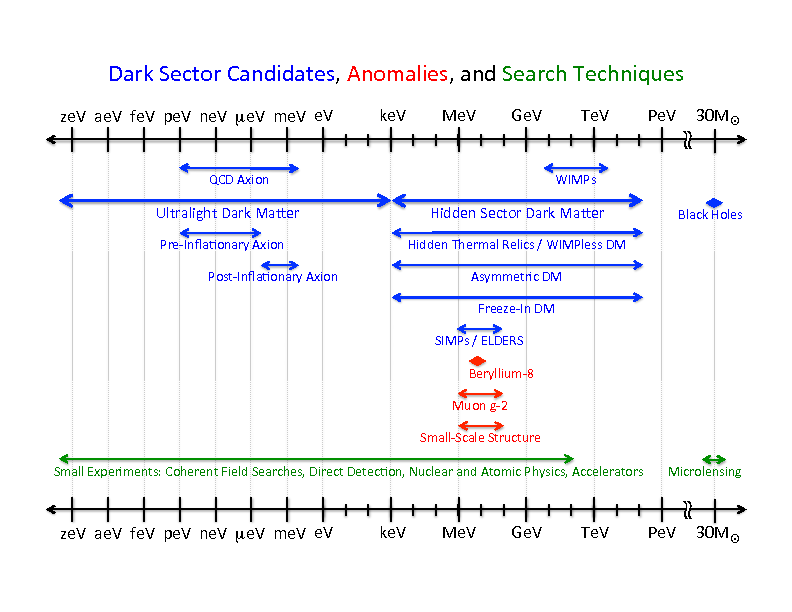
\includegraphics[scale=0.5]{\pdirone/DM_summary.png}
  \caption[Mass range for Dark Matter]{Mass range for Dark Matter and mediator particle candidates, experimental anomalies, and search techniques \cite{battaglieri2017cosmic}.}
  \label{fig:dm-mass-range}
\end{figure}

Because of the relatively loose constraint, it comes to no surprise that a vast amount of models have been theorized for the explanation of DM. The ones depicted in Fig.\ref{fig:dm-mass-range} are only a subset of what is possible, most of time by changing cleverly the model you can make it survive in scales were originally the model was not covered. It is the case for Axion Like Particles (ALPS), that are an extension of the QCD Axion model originally developed to solve strong CP problem \cite{PhysRevD.16.1791}. Contrary to Axions, their mass $m_a$ is taken as independent parameter from their main coupling $g_{a \gamma \gamma}$, and can be arbitrary large. Indeed this mass can also be in the \mev-\gev scale, in the range where the NA64 experiment is sensitive. As we will show in Sec.\ref{ch4:sec:exclusion limits}, we already used out data to constraint a portion of this parameter space \cite{Banerjee:2020fue}.

This thesis does not aim to cover in detail each model of Dark Matter, which is a subject worth a thesis of its own. The avid reader can take a look the following reviews for this purpose \cite{battaglieri2017cosmic,Profumo:2019ujg,HAMBYE2020135553,alex2016dark,review-particle-physics,Feng:2010gw}. Here, we provide a short description of the mainstream possibilities currently considered for Dark Matter:
\begin{itemize}
\item \textbf{\textit{WIMP}}: For a long period of time, Weakly Interacting Massive Particles (WIMP) were considered the most probable candidate by the scientific community. Their main characteristic is tree-level interaction with the W and Z boson, but not with gluons or photons. Historically, their mass is in the 10 \gev-\si{\tera\electronvolt}, although more recent models extended the mass range to lower masses as well. The so-called WIMP miracle \cite{Chang:2013oia}, provided a very effective and natural way to introduce Dark Matter in the thermal history of the early universe in a way that predicted to a very good degree the current relic density. However, after an extensive amount of research, accelerators and direct search have to this date failed to provide evidence to their existence \cite{Arcadi:2017kky}. These models have yet to be ruled out completely, and the remain to this date the most studied type of Dark Matter.
\item \textbf{\textit{Axions}}: Axion and Axion-like particles are obtained by introducing a new pseudoscalar field $a$ with coupling to photons \cite{Marsh:2015xka}. Originally Axions were motivated by the strong CP problem and they were predicted to be extremely light ($<$\si{electronvolt}). The model was later extended to offer a possible explanation for Dark Matter at higher masses. Several experiment based on the "light shining through a wall" concept or using a magnetic helioscope \cite{annurev.nucl.56.080805.140513} already put some stringent limits on Axions. Axion-like particles on the other hand can have a mass large enough to allow testing using accelerators.
\item \textbf{\textit{Sterile Neutrino}}: While Standard model neutrinos are not a good fit to explain Dark Matter as the are produced very hot in the early thermal bath, Sterile neutrinos are on the other hand a viable explanation. Models for this particle vary greatly, and some of the most attractive, like the ones that explain the light neutrinos masses as consequence of the \textit{see-saw} mechanism, are not a viable explanation for Dark Matter \cite{Feng:2010gw}. Nevertheless, models that explain observation do exist, and can be probed by direct detection experiments. To date, no credible signal has been observed.
\item \textbf{\textit{Dark Sector}}: By the name of Dark Sector, we describe a very large class of model characterize by particles not charged directly under strong, weak, or electromagnetic force \cite{alex2016dark}. Particles can still interact with the SM particle through additional interactions constraint by symmetry of the standard model. This are typically called "portals" interactions. This class of models, specifically the ones charged under a new U'(1) symmetry, are the focus of the NA64 experiment, and they will be described more in detail in Sec.\ref{ch1:sec:dm-sector}-\ref{ch1:sec:dm-u1model}
\end{itemize}

In this thesis, the class of models known as Dark Sector will be the focus. To build an experiment it is indeed instructive to focus on a particular signature predicted by a specific mode, in our case the U'(1) model. However, the opposite can still apply, i.e. a specific signature can turn out to be useful to constraint model not in the original scope of the experiment. It the case for the Axion-like particle, that are constraint by the NA64 experiment even though the original goal was to probe the Dark Photon. In summary, one should not think about the data produced by NA64 as exclusively powerful to constraint a single model, but should them freely in the broader framework of new physics.

\subsection{Thermal Dark Matter}
\label{ch1:sec:dm-thermal}

\subsection{The Dark Sector}
\label{ch1:sec:dm-sector}

Dark sectors , introduced in Sec.\ref{ch1:sec:dm-candidates}, are very interesting candidates to explain the origin of Dark Matter (see \cite{battaglieri2017cosmic,alex2016dark} for recent reviews). On the top of reproducing the observed DM abundance in freeze-out or freeze-in scenarios, many experimental anomalies currently observed can be explained inside this framework. The anomalous magnetic moment of the muon \cite{blum2013muon}, the proton charge radius \cite{Pohl2010} and more recently the $\DMX$-anomaly \cite{Krasznahorkay:2015iga,Krasznahorkay:2019lyl} have been suggested as possible hints of a dark sector \cite{alex2016dark}. The definition of this sector is extremely broad, and can accommodate many different models. Its physics however, can be explored effectively and in a systematic way by using specific portal interaction as classification scheme.  The existence of a mediator acting as a portal is not necessary in the Dark Sector, but it natural to select such models in the context of particle physics experiment, as they will be the one with some detectable signature\footnote{If we want to use these models to explain experimental anomalies on the other hand, the existence of a mediator becomes a necessity!} \cite{prw, pospelov}. The gauge and Lorentz symmetries restricts the ways in which the mediator can couple to SM particles. We can classify them using their spin and parity, and by excluding dimension operators larger than 5 we obtain four renormalizable possibilities \cite{alex2016dark}:

\begin{equation}
  \label{eq:dm-portals}
  \mathcal{L} \quad \supset \quad
\begin{aligned}
  &-\frac{\epsilon}{2 \cos{\theta_W}}B_{\mu \nu}F'^{\mu \nu}, &\textrm{vector portal}\\
  & (\mu \phi + \lambda \phi^2)H^{\dagger}H, &\textrm{Higgs portal}\\
  &y_n LHN, &\textrm{neutrino portal} \\
  &\frac{a}{f_a} F_{\mu \nu} F^{\mu \nu}, &\textrm{axion portal}
\end{aligned}
\end{equation}

In this work, we will limit the discussion on the vector portal, as it is the most viable for thermal models of LDM. If we assume the DM mediator to be a vector boson arising from an additional U'(1) gauge group under which the LDM is charged, we can derive a term $\epsilon / \cos{\theta_W} B^{\mu \nu} F'{\mu \nu}/2$ that is invariant both on this symmetry and the well known U(1) from QED. This model can be used to explain the phenomenology of a large class of models, such as scenarios where the Dark Photon couples preferentially to Baryonic, leptonic, or (B - L) currents. One such case, where the coupling to Baryon is disfavored, is the protophobic $\DMX$ gauge boson \cite{PhysRevD.95.035017}. Additionally, the DM could also have a Majorana couplings to the mediator \cite{PhysRevD.93.063523}, or it could live in a rich sector \cite{Morrissey_2014}.

From here on we will shift the discussion on more practical terms, which means describing a minimal model of dark gauge vector boson and calculate its yield in a particle physics experiment. This model can be easily extended to more complex scenario by adding constraint and terms on the Lagrangian. We remind here, that today the progress on experimental results started to put heavy constraint on this parameter space, thanks as well to the NA64 efforts, excluding even important models like the one capable of justifying the anomalous magnetic moment of the muon. This constraint have been placed by beam dump \cite{jdb, charm, rio, e137, konaka, bross, dav,  ath, nomad, e787, essig1, blum,sg1, blum1, sarah1}, fixed target \cite{apex,merkel,merkel1}, collider \cite{babar, curt, babar1}, rare particle decay searches \cite{sindrum, kloe, sg2, kloe2, wasa, hades, phenix, e949, na48, pol, kloe3} and the new determination of the fine structure constant $\alpha$ combined with the measurement of $(g-2)_e$ \cite{Parker191,PhysRevLett.100.120801}.

\section{The U'(1) model}
\label{ch1:sec:dm-u1model}

A possibility is that this new force is carried by a vector boson $A'$, called dark photon.
Stringent limits on the coupling strength $\epsilon$ and mass $m_{A'}$ of such dark photons, excluding the parameter space region favored by the anomalous magnetic moment of the muon, the so called $(g-2)_{\mu}$ anomaly, have already been placed by 

\begin{equation}
  \label{eq:dm-rate}
  N_{\DM} \sim N_{EOT} \times C' \epsilon^2 \frac{m_e^2}{m^2_{\DM}}
\end{equation}

\subsection{Decay modes}
\label{ch1:sec:dm-decay}

\subsubsection{Invisible decay mode}
\label{ch1:sec:dm-decay-invis}

\subsubsection{Visible decay mode}
\label{ch1:sec:dm-decay-vis}


\begin{eqnarray}
  L_{\DM} = 28.3 ~{\rm mm}  \Bigl[\frac{E_{\DM}}{100~ {\rm GeV}}\Bigr] 
  \Bigl[\frac{17~ {\rm MeV}}{m_{\DM}}\Bigr]^2 \Bigl[\frac{10^{-3}}{\epsilon}\Bigr]^2
  \label{eq:dm-decay-length}
\end{eqnarray}

\subsection{The X17 anomaly}
\label{ch1:sec:dm-u1model-motivations-x17}

A great boost to search for the new light boson weakly coupled to Standard Model particles was triggered by the recent observation of a $\sim$7$\sigma$ excess of events in the angular distribution of $\pair$ pairs produced in the nuclear transitions of the excited $^8$Be$^*$ nuclei to its ground state via internal $\ee$ pair creation \cite{Krasznahorkay:2015iga}. The latest results of the ATOMKI group report a similar excess at approximately the same invariant mass in the nuclear transitions of another nucleus, $^4$He \cite{Krasznahorkay:2019lyl}.

It was put forward  \cite{Feng:2016jff,PhysRevD.95.035017}, that this anomaly can be interpreted as the emission of a protophobic gauge boson $\DM$ decaying into $\pair$ pairs. To be consistent with the existing constraints, the $\DM$ boson should have a non-universal coupling to quarks and a coupling strength with electrons in the range of $2\times 10^{-4} \lesssim \epsilon_e \lesssim 1.4\times 10^{-3}$ which translates to a lifetime of the order of $10^{-14}\lesssim \tau_X \lesssim 10^{-12}$~s. Remarkably, this model also explains within experimental uncertainty the new result obtained with the $^4$He nucleus, providing both kinematical and dynamical evidence to support this interpretation \cite{Feng:2020mbt}. This model will be used as benchmark for the NA64 current results and to cast the sensitivity of the new setup described in this article. However, other solutions of the $\DM$ anomaly were proposed, see for example \cite{Nam:2019osu, Seto:2016pks}.

Interestingly, such a new boson with a relatively large coupling to charged leptons could also resolve the tension between measured and predicted values of the $(g - 2)_{\mu}$. In addition to vector and axial-vector explanation of the $\DM$ anomaly, one can consider scenarios involving hidden pseudo-scalar boson \cite{Ellwanger:2016wfe}. Corresponding pseudo-scalar couplings to electrons satisfy existing experimental constraints \cite{Andreas:2010ms,Adler:2004hp}. An analysis to probe such pseudo-scalar states at NA64 \cite{Kirpichnikov:2020tcf} would require a proper Monte-Carlo simulation of the spectra and flux of light pseudo-scalar boson produced in the target by electrons.
Another interesting result comes from the new measurement of $\alpha$ performed by Parker et al. \cite{Parker191} which combined with the $(g-2)_e$ measurements result in a 2.4$\sigma$ deviation from the QED predictions \cite{PhysRevLett.100.120801}. Should this tension be confirmed, the two constraints coming from the NA64 results and $(g - 2)_e$ would exclude the vector and axial vector couplings explanation of $\DM$. On the other hand, models with nonzero V$\pm$A coupling constant with the electron would explain both electron and muon $(g - 2)$ anomalies \cite{Krasnikov:2019dgh}. In these models, the $\DM$ could have a coupling of $6.8\cdot 10^{-4} \lesssim \epsilon \lesssim 9.6 \cdot 10^{-4}$ which leaves an interesting region of the parameter space to be explored.
These models motivated the study of the phenomenological aspects of such a light vector boson weakly coupled to quarks and leptons (see, e.g., Refs.~\cite{fayet1, fayet2, fayet3, fayet4,jk, cheng, Zhang:2017zap, ia, liang, bart}) 
and new experimental searches (see e.g., Refs.~\cite{battaglieri2017cosmic, nardi}).

Recently, the NA64 collaboration has reported new results that excluded the $\DM$ boson  with the coupling strength  to electrons in the range $1.2 \times 10^{-4} < \epsilon_e < 6.8 \times 10^{-4}$ \cite{Banerjee:2018vgk,Banerjee:2019hmi}, by using the calorimeter technique proposed in \cite{Gninenko:2013rka,Andreas:2013lya}. In this work, the main challenges to search for large coupling $\epsilon \sim 10^{-3}$ of $\DM$ will be outlined and an upgrade of the setup to overcome them is described. First, in Sec.\ref{ch3:sec:vis-mode-veto} an overview on the calorimeter method \cite{Gninenko:2013rka,Andreas:2013lya,Banerjee:2019hmi} is presented and the main limitations of the current setup are outlined. In Sec.\ref{ch3:sec:vis-mode-tracking}, a new analysis method that exploits the trackers is presented. This analysis highlights the importance of an efficient tracking procedure for the $\DM$ search. The increase in sensitivity is however negligible due to the intrinsic limitations of the setup.

%%% Local Variables:
%%% mode: latex
%%% TeX-master: "../PhDthesis"
%%% End:

% Chapter 2

% variables
\newcommand{\pdirtwo}{chapters/plots/chapter2}

\chapter{The NA64 experiment} % Main chapter title

\label{chapter2} % For referencing the chapter elsewhere, use \ref{Chapter2} 

% ----------------------------------------------------------------------------------------

Now that a general introduction about the Dark Matter problem was given and we detailed some basic formula to calculate the rate expected in a fixed-target experiment, we are ready to describe the NA64 setup in detail. As the first step, we will clarify what are the main requirements for each of the two decay channels that are being probed by the NA64 experiment. This is be discussed in Sec.\ref{ch2:sec:experimental-technique}, where the experimental method is outlined together with the possible challenges to be solved. Conceptually speaking, the two setup shares many similarities, and indeed it is straight-forward to modify one into the other by adding a few more detectors. In the case of invisible mode, a single calorimeter is used as an active target to trigger the $\DM$ production, which is assessed by missing momentum in the final state. In the visible mode, a second calorimeter is placed downstream the main target, and the production of $\DM$ is detected by matching the energy of the $\ee$ in the $\aee$ decay with the one deposited by the initial em-shower inside the active dump. In both cases, a well defined initial state is required, together with a longitudinal hermeticity to avoid any energy leak. In Sec.\ref{ch2:sec:experimental-setup} an accurate description of both the two setups is given, and we will try to give a practical answer to the challenges outlined in the first section. The initial particle momentum is measured using a magnetic spectrometer with high-resolution tracking stations. The energy is then reconstructed in an active target segmented both longitudinally and transversely. The precise energy deposited in each cell is used to characterize the incoming particle ID. For the same purpose, Synchrotron Radiation emitted during the passage through the magnetic field is also measured and used to distinguish electrons from the hadronic and muonic contamination of the beam. An introduction of the different types of triggers is then provided to help the reader distinguish between data collected at different conditions. These are needed to differentiate between runs used for the $\DMX$ searches and run used to test the detector's responses and the reliability of MC-simulations.
Finally, a detailed description of each detector is given in Sec.\ref{ch2:sec:detectors}, to provide all the technical details of the detectors used in NA64. 

\section{Experimental Technique}
\label{ch2:sec:experimental-technique}

The detection of the $\DM$ needs to follow different strategies depending on the dominant branching ratio. If $\DM$ decays mainly into $\dmchi$, one could try to detect one of the two particles using a very thick detector. Indeed this is possible since by definition in the $\umodel$ a portal exists that connects dark matter to the classical one. However, such an experiment will have a very limited reach, not only a factor $\alpha \epsilon^2$ needs to be "paid" to produced $\DM$ but an additional $\alpha \epsilon^2$ is also needed to detect its decay products. For low couplings $\epsilon$, the probability to detect a single $\DM$ becomes vanishingly small. The second possibility is to make the disappearance of energy the signal of the experiment, i.e. assuming that the energy of $\DM$ is completely lost in the event. Such an experiment needs only to produce $\DM$ and does not need to worry about what happened to the particle after. To design a setup able to characterize this type of signature properly, we need to worry about the following items:

\begin{itemize}
\item The initial momentum of the particle needs to be well known
\item The setup needs to be completely hermetic, i.e. no energy can escape detection without using the channel 
\item The initial particle ID needs to be well known
\end{itemize}

While the two first item are fairly trivial, one could wonder why the last one is necessary. If we need to apply any kind of statistical analysis to our data one has to know the total number of the electron that impacts our target, the so-called Electron On Target (EOT), so in this sense to understand the sensitivity of the experiment such knowledge is necessary. The particle ID is necessary also to distinguish events that are in our signal box even if no $\DM$ is being produced. A precise background discussion is left for chapter \ref{chapter3}, here we just provide the example of the decay chain $K^- \to e^- \nu_e$ \cite{review-particle-physics}: if a $K^-$ hits the target without being properly distinguished, it can leave an electromagnetic signature and at the same time transport some energy out of the setup via the $\nu_e$. This is exactly the signature we would expect for $\DM$! Hence the necessity of some system able to distinguish between particles of different species.

What about the visible mode? If we assume the decay $\aee$ is dominant, it is clear that missing energy can no longer be considered a signature. One should instead search for a $\ee$ pair in the final state, these particles are however very common in a particle physics experiment, so one has to think how to characterize the event more. The property that mostly distinguish dark matter is its low coupling with ordinary matter, that allows it to travel inside very dense material with no interaction. Since $\DM$ travels for a finite distance before decaying, if the target is thick enough, the only way to see an $\ee$ emerging from the target will be that a $\DM$ is being produced. A simple $e^-$ will be stopped by the thick target, and nothing will emerge on the other side of the wall. If on the other hand, we measure a high-energetic $\ee$ pair on the other side of the wall and the energy of this pair matches exactly the one that is missing from the target, we conclude that the energy was transported outside the volume using a neutral boson. Assuming that no such channel exists in the standard model (which is to be demonstrated with a detailed background study) we can claim the observation of an event compatible with our hypothesis! Noticed in this case as well the three properties listed above are necessary: one needs to know with good precision the initial momentum of the particle hitting the target and be sure that the particle is an electron. In this case, however, the signal is not missing energy, but instead energy conservation between a detector placed upstream and the one placed downstream. This concept is similar to what is used for Axion searches, the so-called "Light Shining Through a Wall" experiments, where the two photons of the Axion decay are detected downstream a very thick wall (for a review, look here \cite{Jaeckel:2010ni}).
If we assume the energy of the primary electron to be $E_0$ and we plot the energy recorded in the two calorimeters, we can conceptualize the difference between the two signature in Fig.\ref{fig:two-signature}. As one can see, we are assuming here that the first calorimeter can stop the incoming particle with 100\% efficiency, and that therefore the only way to reach the downstream calorimeter is via the production of dark matter. Although this is mostly the case if the incoming particle is an $e^-$, to probe the $\umodel$ one has to collect a huge number of EOT, in the order of $10^{12}$. When a statistic so large is collected, background can arise from very unlikely interactions not straightforward to compute. A good setup should not only implement the fundamentals described above, but also suppress as much as possible all the background that can potentially leak in the signal box.

\begin{figure}[bth!]
  \centering
  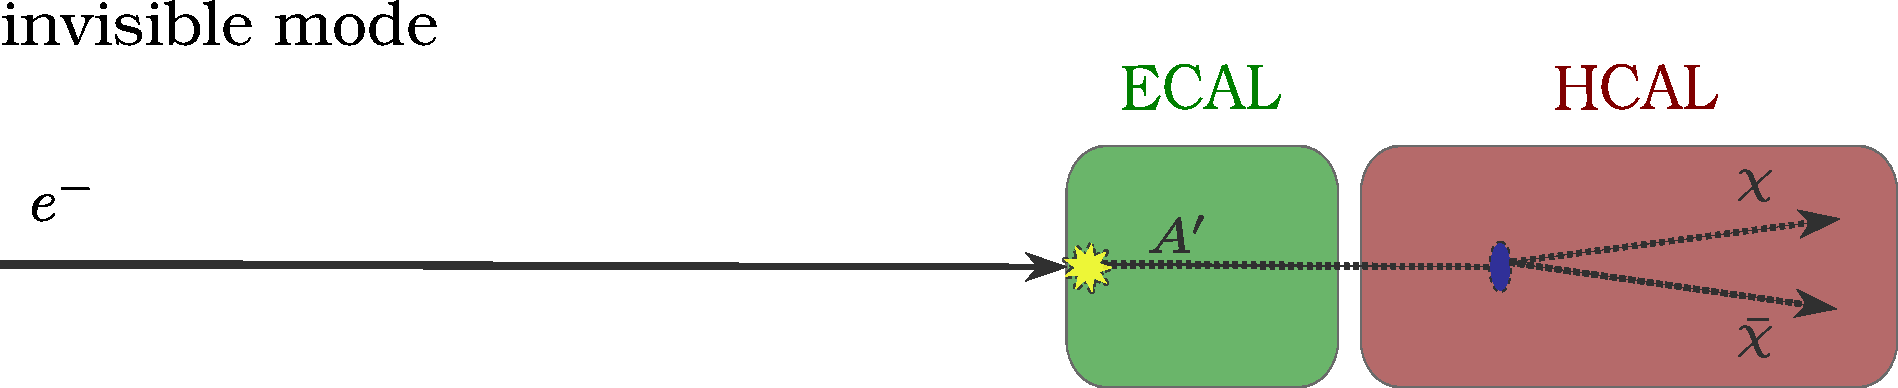
\includegraphics[width=\textwidth]{\pdirtwo/experiments-concepts-invisible.pdf}
  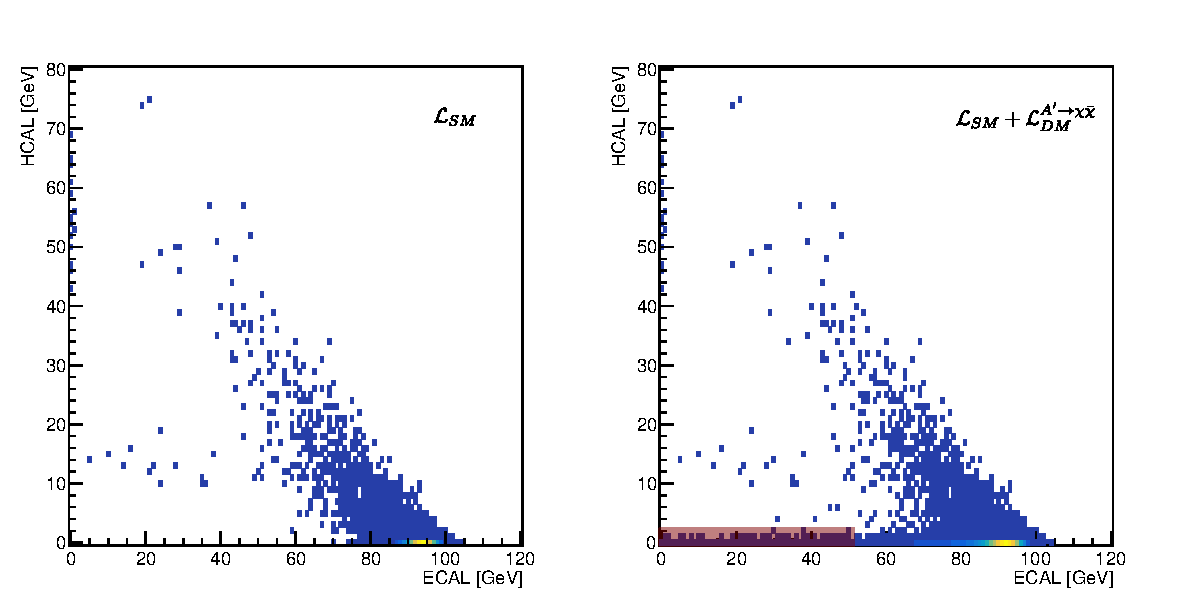
\includegraphics[width=\textwidth]{\pdirtwo/invisiblemode_signalregion.pdf} \\
  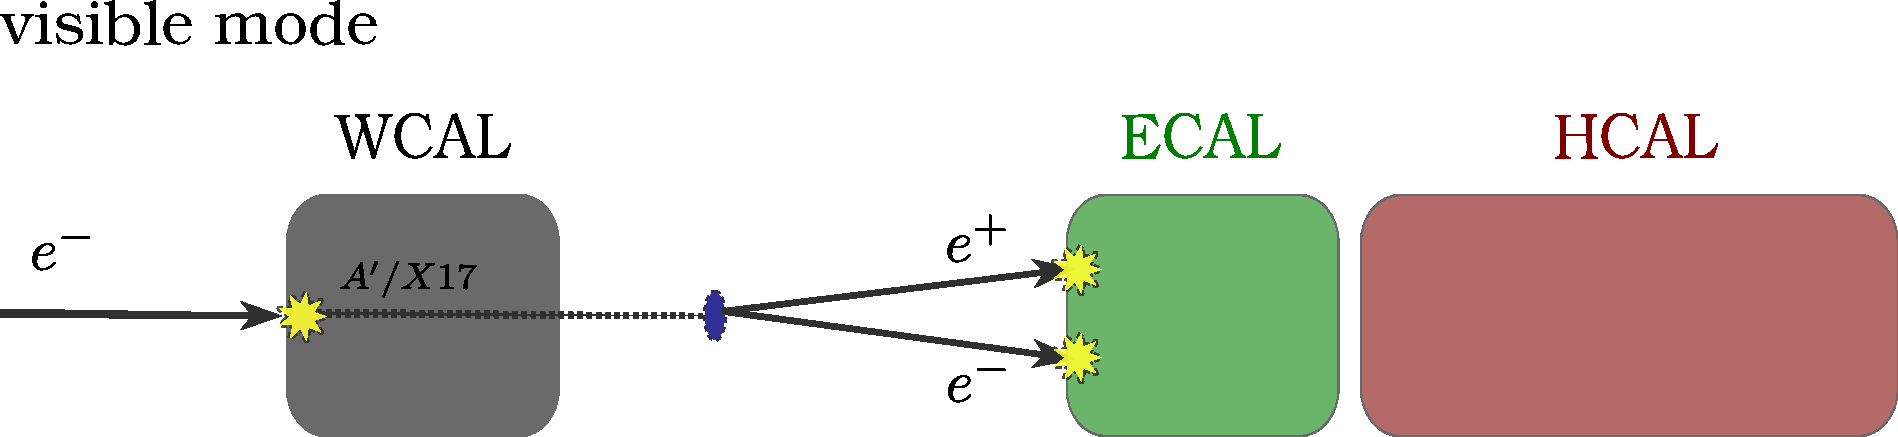
\includegraphics[width=\textwidth]{\pdirtwo/experiments-concepts-visible.pdf}
  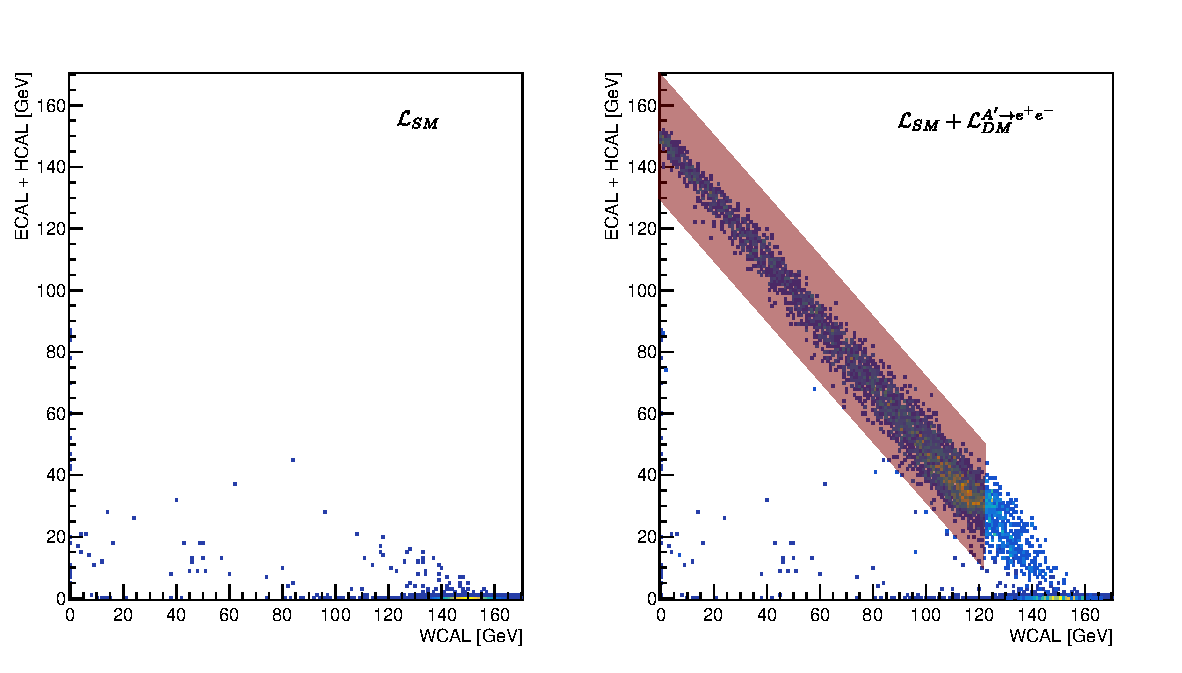
\includegraphics[width=\textwidth]{\pdirtwo/visiblemode_signalregion.pdf}   
\caption[Sketch of experimental signatures for $\DM$]{Sketch of the two possible signature in a collider setup to probe the $\DM$ existence. A heatmap present the event distribution in the two setups, using only standard model physics (left column) and after adding an additional U'(1) in the simulation. This is done assuming invisible mode decay $\ainv$ (top) or visible mode decay $\aee$ (bottom). In both cases, the signal region of the experiment is drawn as a shaded area.}
\label{fig:two-signature}
\end{figure}

\clearpage
\newpage

\section{Experimental setup}
\label{ch2:sec:experimental-setup}

In collider experiments, the first choice of a facility to provide the initial beam for the experiment can be crucial. A good initial beam with a low fraction of impurities and good momentum definition can change significantly the background conditions. The NA64 experiment uses the upgraded H4 electron beamline at CERN SPS. The beam is produced by the primary proton beam of 450 \si{\giga\electronvolt} with an intensity up to 10$^{12}$ Proton On Target (POT) per SPS spill. The electrons are produced on a primary beryllium target and transported to the detector inside the evacuated beamline tuned to an adjustable beam momentum. A precise description of the beam apparatus is available here \cite{sps-beamline,h4-beamline}. The beam properties can be tuned, hence its precise output depend on the target used for the conversion, the magnetic field settings, and other parameters. In the case of NA64, two different compositions are used depending on which $\DM$ decay channel is being probed. In the case of the invisible decay $\ainv$, the beam momentum is tuned to 100 \gev. In this condition, a purity $\pi^-/e^- \lesssim 10^{-2}$ is achieved with a beam size of $\sim$1.5\si{cm} (FWHM). In the case of the visible decay $\aee$ on the other hand, large initial energy can be helpful to boost the decay time of the $\DM$ to increase its chances of traveling outside the target. This is especially true for the $\DMX$, since an important portion of the parameter space justifying this anomaly is characterized by large coupling $\epsilon \gtrsim 10^{-3}$ and hence a decay time $\tau \lesssim 10^{-13}$\si{s}. In this case, the beam is tuned to 150 \gev as a compromise between high-energy and small beam degradation.

In the next sections, both of the setup used by NA64 will be described in detail. Since the physics happening is the same before the electron hits the target, the two setup shares many similarities. We will follow here a historical approach where we will describe first the invisible mode setup which was first used in the test beam of 2016. In Sec.\ref{ch2:sec:vismode} on the other hand we will focus on the most important difference between the two setups.


\subsection{The invisible mode setup}
\label{ch2:sec:invismode}

The NA64 invisible mode setup has changed slightly during the year as the understanding of the specific problems in the $\DM$ search was discovered. In the interest of time, we will here describe the most updated version of it, that was used in the data taking of 2018.

After the 100 \gev e$^-$ enter the setup, its momentum needs to be measured precisely to provide an initial estimate of its energy. This is achieved using a magnetic spectrometer using an integrated field of $\sim 7$ \si{\tesla\meter} achieved using two dipole magnets \cite{mbpl} placed in series along the primary axis of the beam. The entrance angle of the particle inside the magnet is defined by two Micromegas (MM) trackers placed inside the 5 m space between the beam inlet and the first magnet entrance. Between the two MM, in a space of approximately 2 m, two scintillators ($S_{0-1}$) and a V counter are placed to ensure a proper beam definition. The V counter consists of a scintillator with a hole in the middle and is used to reject particle with a high beam divergence that could in principle be a source of background. After the two magnets, a vacuum tube kept at the pressure of approximately 10$^{-3}$ \si{mbar} is placed immediately after for a total length of 10.2 \si{m}. The vacuum tube minimizes the interaction of the particles during its travel to the target. This is important to reduce the energy loss of the primary e$^-$ before its energy is measured again in the ECAL, but as will be detailed in Sec.\ref{ch3:sec:bkg-srd}, reducing the ionization improves as well the background suppression achievable with synchrotron radiation. After the vacuum tube, additional space of $\sim$ 4.5 \si{m} contains the last detector before the target. A second set of three scintillators ($S_{2-3-4}$) completes the triggers. Three sets of Pb-Sc sandwiches are placed in the arch contained between the original beam and the bent beam direction to collect the synchrotron radiation emitted in the magnetic field upstream. On the other side of the beam, another similar detector with no transversal segmentation (W sandwich) is placed to reject events with high beam divergence or where the electron experienced an high energy scattering upstream. Four more MM (MM$_{3-4-5-6}$) are placed along the beam to complete the momentum reconstruction by detection of the precise hit position of the electron after its passage through the magnetic field. Eight more tracking detectors are placed before the ECAL: 2 Strawtubes (St), 2 Hodoscope (H), and 4 four Gas Electron Multiplier (GEM). The GEM detectors have a hit resolution and efficiency similar to the MM, with the advantage of not being multiplexed, hence they experience less redundancy in the hit position. As it will be detailed in Sec.\ref{ch2:sec:detectors-tracking}, the multiplexing does not limit the momentum resolution and hence the final performance given are comparable overall. The straw tubes and Hodoscope, on the other hand, posses a larger active area ($\sim$0.5 m), but a hit resolution of $\sim$1 \mmi which makes them less suitable to reconstruct the momentum precisely \cite{Volkov:2019qhb}. This detector have however the virtue of being large enough to detect charged particle emitted at a large angle, and hence can reject some rare events that are produced by inelastic scattering of the incoming particles on one of the MM modules placed downstream. These events are not rejected by the W alone and they can be a source of background for the large number of EOT required by the experiment \cite{na64-prd}. 

After this region is passed, the primary electron hits the active target (ECAL). Here the energy of the electron is measured again by stopping the particle completely. The ECAL is made of 36 modules arranged in a 6$\times$6 matrix, each module has a Pb-Sc structure with 150 layers for a total of 40$X_0$. Due to its transverse segmentation, the ECAL allows further background rejection using a shower profile analysis to distinguish between an em-shower and a hadronic one. To ensure complete hermeticity, a high-efficiency VETO and a large Hadronic Calorimeter (HCAL) are placed after the ECAL target. The VETO consist of three separate scintillators stacked together for a total thickness of 5 \si{\centi\meter} and reject MIP with an estimated efficiency of 99.9$\pm$0.1\%. The HCAL, placed immediately after, consist of four modules of $\simeq$7 $\lambda_{int}$ (nuclear interaction length) each. Each module is built in a 3$\times$x matrix of a single Fe-Sc sandwich array. The role of this last calorimeter is to block all possible particles penetrating the ECAL and grants complete energy hermeticity. In the past version of the setup, all four modules were stacked in series after the ECAL to grant a total of $\simeq$28 $\lambda_{int}$ \cite{Banerjee:2016tad}. In the more recent installment however, the last module is shifted to face the original beam axis (Fig.\ref{fig:setup-invis-2018}). After the first test beam, it was clear that the additional background suppression of a fourth module was not needed. Instead, the last module is used to gain insight into the neutrals in the beam and can catch large bremsstrahlung photons emitted before the magnet by the incoming electrons. A more detailed description of all this detector can be found in \ref{ch2:sec:detectors}.

\begin{figure}[tbh!]
  \centering
  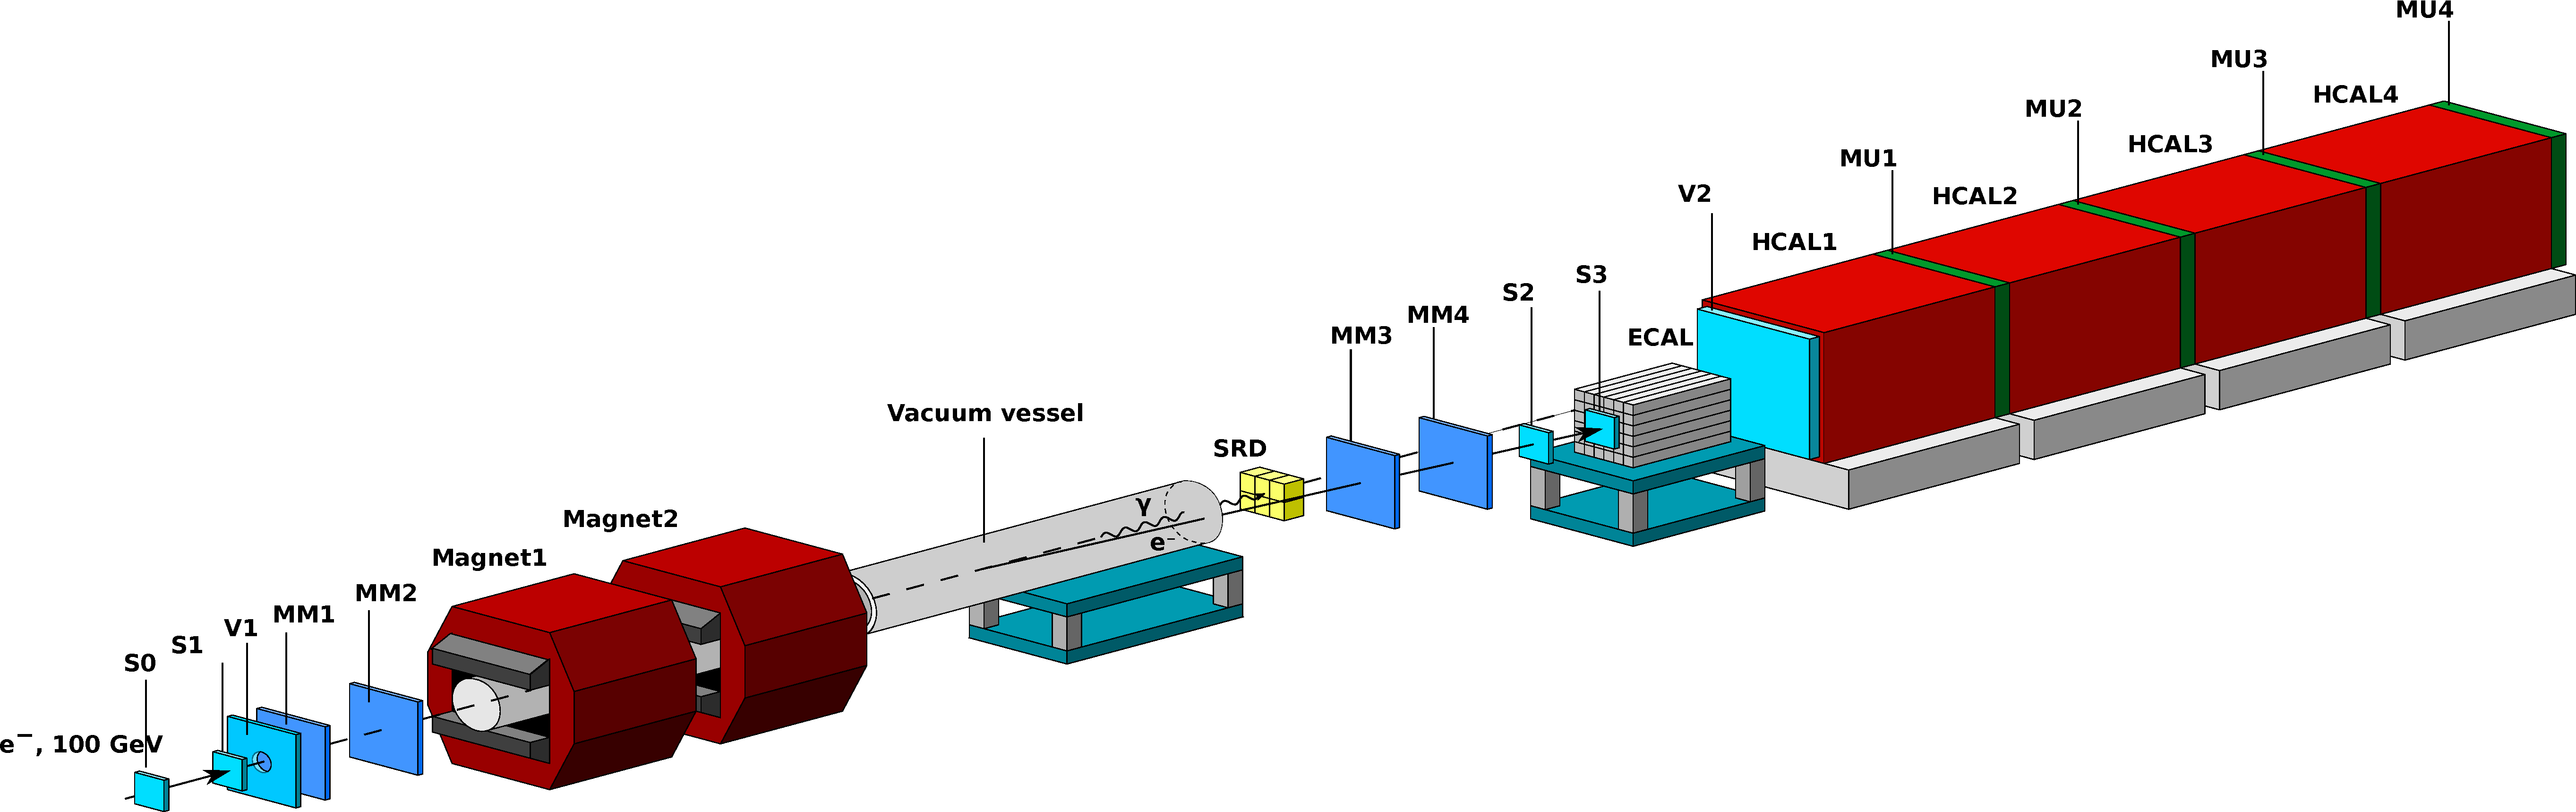
\includegraphics[width=\textwidth]{\pdirtwo/invisible_mode_setup.pdf}
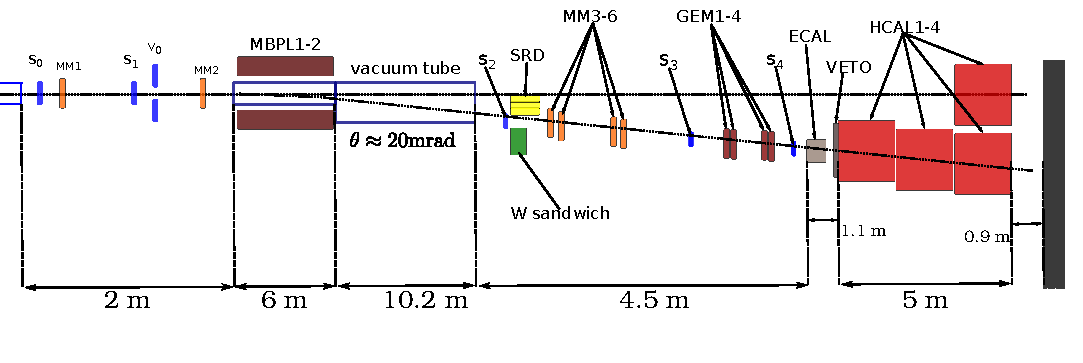
\includegraphics[width=\textwidth]{\pdirtwo/setup-invis-2018.pdf}
\caption[invisible mode setup 2018]{Top: Invisible mode setup sketched in 3D. Main detectors are shown. Dummy decay of a $\DMX$ after the dump is depicted. Bottom: Top view of the invisible mode setup used in 2018, all detectors included.}
\label{fig:setup-invis-2018}
\end{figure}

\subsection{The visible mode setup}
\label{ch2:sec:vismode}

The visible mode setup is obtained by modifying slightly the invisible mode setup to accommodate the $\aee$ decay in a long decay volume where the $\ee$ pair is measured by a scintillator counter and four GEM station (Fig.\ref{fig:setup-vis-2018}). The energy of the beam is increased to 150 GeV\footnote{First run in 2017 was performed at 100 \gev.}. The reason for this is to boost the decay time of the $\DMX$ to increase its probability to leave the dump. As a consequence, the total displacement in the X-direction of the primary beam is roughly $\sim$10 \si{mm} smaller. Since the space between the origin and bent beam axis is reduced, only two modules of the SRD detector can be placed in this space, which decreases the suppression of heavy charged particles. Additionally, the smaller bending has an impact on the momentum reconstruction as well, this however less significant for this analysis: since no energy evaporates in this mode, there is no direct need to compare two different energy measurements. Instead, another compact calorimeter made of a Tungsten-scintillator sandwich (WCAL) is placed in front of the ECAL and acts as the target in this new setup. This calorimeter has a total of 30$X_0$ in a compact length of $\sim$20 \si{cm}. The $\DM$ is produced via scattering off nuclei in this active dump, followed by its decay $\aee$ after traveling for some distance without interaction. To ensure that the decay happens after the dump, the last two layers of the WCAL are read separately (W2), and act as a veto to stop high energetic particles that leak from the em-shower to enter the decay volume undetected. A vacuum tube of 3.1 \si{m} kept at a pressure of $\sim$10$^{-2}$ \si{mbar} is placed immediately after the dump to minimize interaction of the $\ee$ after the decay. A scintillator (S$_4$), is placed immediately after the tube to detect the presence of the $\ee$ pair with a double-MIP signal inside this counter. A set of four GEM detectors are then placed in the last $\simeq$2.5 \si{m} of air before the second active target (ECAL). In principle, these four trackers can reconstruct the angle and the vertex of the decay to offer an additional characterization of the signal. These tools were not used in the analysis performed in 2018 \cite{Banerjee:2019hmi}, but in this work, an analysis considering the trackers as well is described (see Sec.\ref{ch3:sec:vis-mode-tracking}). Finally, the ECAL detects the remaining energy of the two $\ee$ pair in the decay volume, and matches it to the one measured in the WCAL. If the sum $E_{WCAL}+E_{ECAL}$ is compatible with the initial primary energy E$_0$, we conclude that some energy escaped the first dump WCAL using a channel not compatible with the standard model of particle physics. At the end of the setup, a high-efficiency VETO and the HCAL are still presented to guarantee again complete hermeticity. One could question the usefulness of these detectors here, indeed if we can guarantee that only 150 GeV $e^-$ are in the system, the simple requirement of energy conservation should be enough to reject all backgrounds coming from impurities in the beam. Again here we need to remember that the many assumptions made in theory can encounter many problems in practice. The pileup of two different events, one hadronic and one electromagnetic could easily break this assumption. The limited energy resolution of the two calorimeters can likewise produce on the rare occasion a wrong measurement that implies energy conservation. On top of this, the HCAL is invaluable to properly estimate the hadron contamination of the beam (and therefore the precise number of EOTs accumulated) and to select the rare event $\emu$ where two muons are produced in the dump inside the em-shower. As we will see this type of event is crucial for our analysis to properly account for the systematic of the experiment, both in the invisible and visible mode, which makes the HCAL and VETO necessary for both setups.

\begin{figure}[tb]
  \centering
  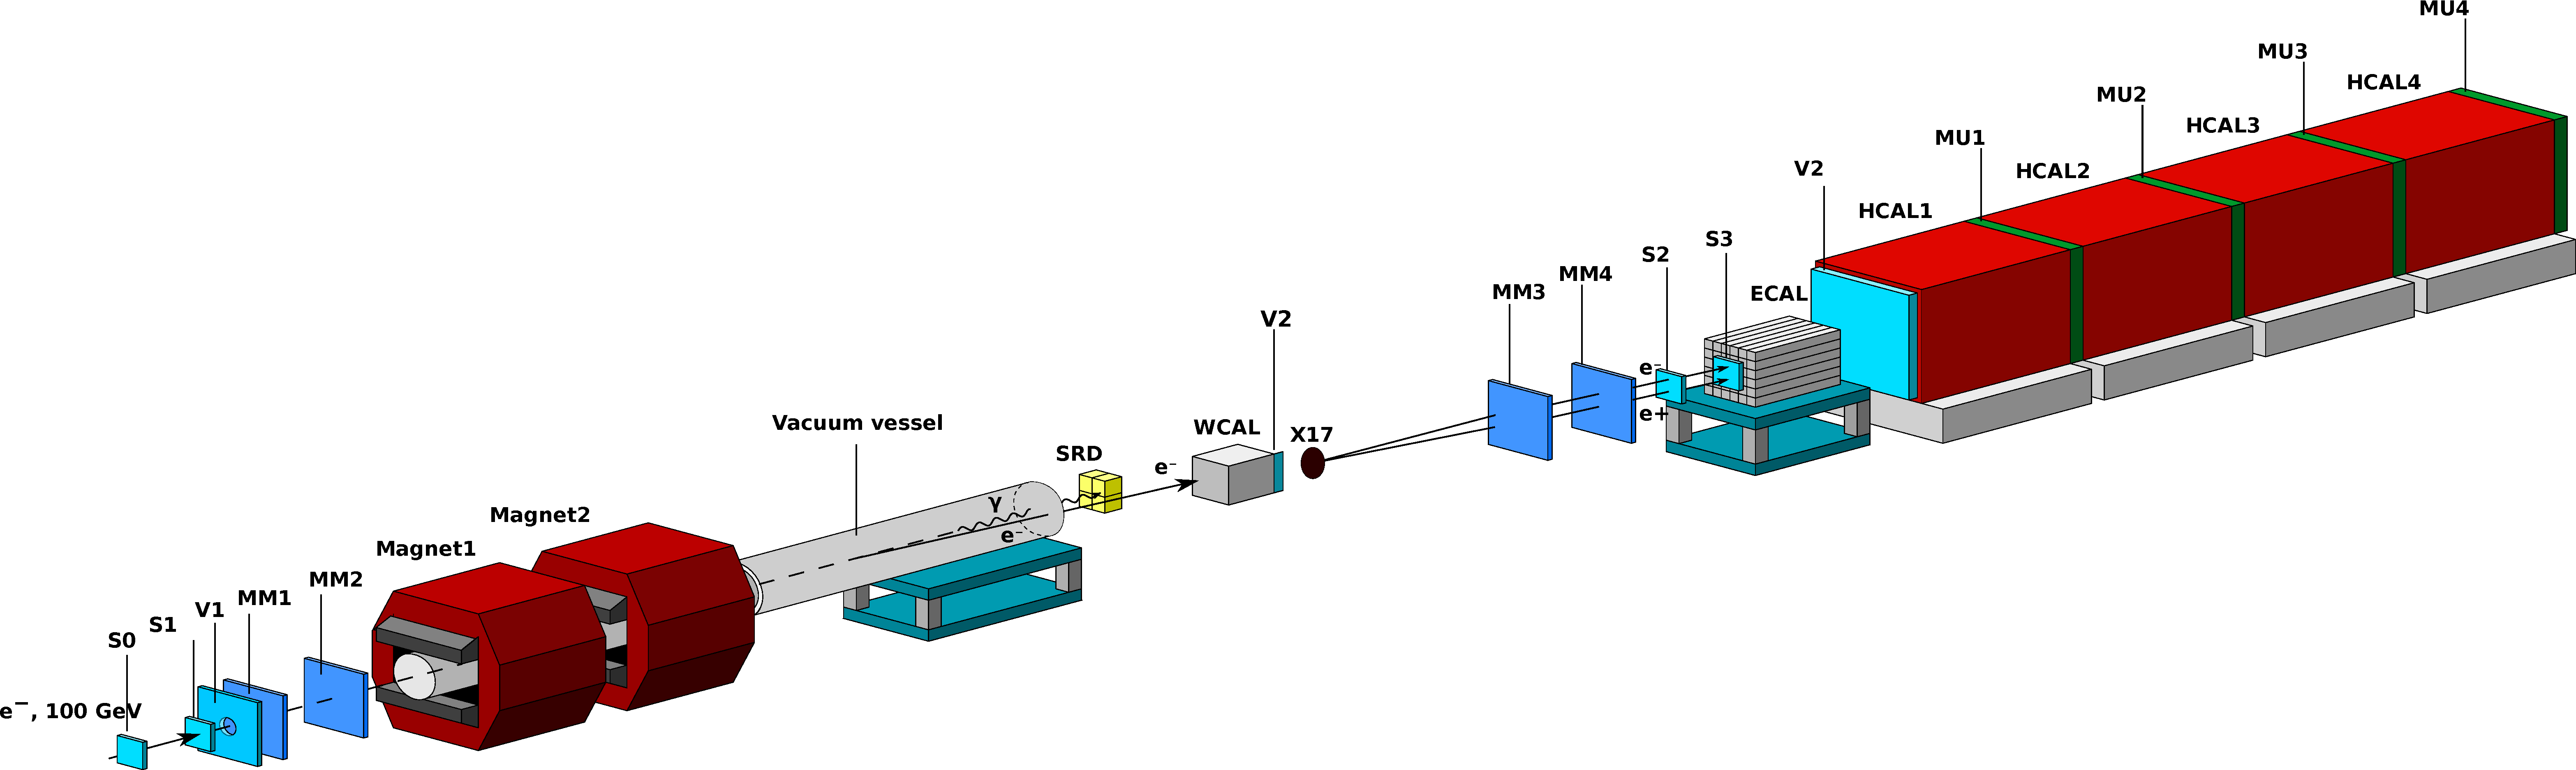
\includegraphics[width=\textwidth]{\pdirtwo/visible_mode_setup.pdf}  
  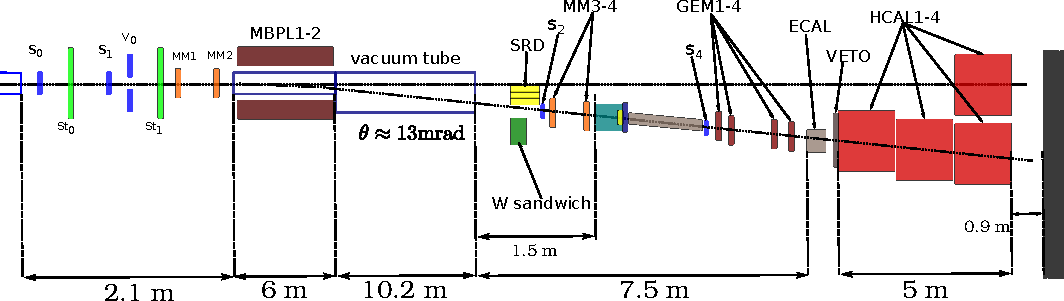
\includegraphics[width=1.\textwidth]{\pdirtwo/NA64_setup_2018_visible.pdf}
  \caption[NA64 visible mode setup 2018]{Top: Visible mode setup sketched in 3D. Main detectors are shown. Bottom: Top view of the visible mode setup used in 2018, all detectors included.}
  \label{fig:setup-vis-2018}
\end{figure}

\section{Detectors}
\label{ch2:sec:detectors}

In this section, the various detectors that are used to build the two setups are described in more detail to give a technical overview of each component. More information about each detectors can be found in \cite{na64-hcal,na64-detectors,ABBON201569}. 

\subsection{The Trigger system}
\label{ch2:sec:detectors-trigger}

The trigger system is based on the coincidence and anti-coincidence of different scintillator counters placed along the beam directions combined with the requirement of specific energy in the primary active dump (the ECAL in the invisible mode and the WCAL in the visible mode).

Five plastic scintillators (S$_{0-4}$) and one Veto (V) are used in the NA64. They have a variable diameter ranging from 32 to 42 \si{mm} and a thickness of 3-5 \si{mm}. The sandwich S$_0$-V-S$_1$ is placed in front of the beam inlet to characterize the initial particle direction. To pass this first step of the trigger, a particle needs to leave a signal of $\sim$0.8 MIP in S$_{0-1}$ and no signal in V, i.e. following the condition:

\begin{equation}
\label{eq:trigger-upstream}
Tr_U = S_0 \cdot \bar{V} \cdot S_1
\end{equation}

The signal needs to be in a coincidence compatible with the time resolution of the two scintillators ($\simeq$3 \si{ns}) to suppress the pileup. Downstream, three more scintillators are placed (S$_{2-4}$) in the case of the invisible mode and a coincidence of all three is also required as a part of the trigger downstream. In the case of the visible mode, only the first of three scintillators (S$_2$) is part of the trigger, S$_3$ is removed and S$_4$ is placed after the decay for analysis purpose without being a direct part of the trigger. This means:

\begin{equation}
\label{eq:trigger-downstream}
Tr^{invis}_D = S_2 \cdot S_3 \cdot S_4
Tr^{vis}_D = S_2
Tr_{U+D} = Tr_U \cdot Tr^{invis/vis}_D
\end{equation}

In this case, we notice that the scintillator S$_2$ downstream is small enough to already limit significantly the range of momenta accepted in the trigger of the experiment ($\gtrapprox$ 90 \si{\gev})). However, large beam divergences coupled to pileup can still potentially cause a low energy $e^-$ inside the trigger window, hence the necessity of a tracking system. As a final tool for the beam definition, a small energy deposit in W is required, to reject events with large upstream bremsstrahlung. The exact threshold is not consistent between different runs, but it is always in the range of 3-6 \gev. We define the beam-trigger as the sum of all these components in the two different setups:

\begin{equation}
\label{eq:trigger-beam}
Tr_{beam} = Tr_{U+D} \cdot \bar{W}
\end{equation}

Finally, as the DAQ can collect data at a rate of $\simeq$10 \si{kHz}, one needs an additional condition to select only those events that have a chance to be in the signal region. In both setups, this means some missing energy in the primary target-dump. Additionally, since both WCAL and ECAL have some longitudinal segmentation, one can use the pre-shower information to suppress the hadron background at the trigger level. This is achieved by splitting the signal in these modules to feed them to a discriminator. The trigger, in this case, has the following form:

\begin{equation}
\label{eq:trigger-phys}
\begin{split}
& Tr^{invis}_{phys} = ECAL^{presh}(>300 MeV) \cdot ECAL(<85 GeV)\\
& Tr^{vis}_{phys} = WCAL^{presh}(>500 MeV) \cdot WCAL(<110 GeV)
\end{split}
\end{equation}

The final trigger during data taking will be a combination of both the primary trigger for the beam definition and the physical trigger used to obtained a rate that can be handled by the DAQ. We obtain finally:

\begin{equation}
\label{eq:trigger-total}
\begin{split}
& Tr^{invis}_{total} = S_0 \cdot \bar{V} \cdot S_1 \cdot S_2 \cdot S_3 \cdot S_4 \cdot \bar{W} \cdot ECAL^{presh}(>300 MeV) \cdot ECAL(<85 GeV)\\
& Tr^{vis}_{total} = S_0 \cdot \bar{V} \cdot S_1 \cdot S_2\cdot \bar{W} \cdot WCAL^{presh}(>500 MeV) \cdot WCAL(<110 GeV)
\end{split}
\end{equation}

The precise definition of the trigger varies between different runs. In general, we can define three different categories:

\begin{itemize}
\item \textbf{Hadron calibration run:} Where $\pi^-$ is used as primary particle and only $Tr_{beam}$ is used. These runs are used to measure precisely the interaction of hadrons in the setup to study precisely the background suppression in NA64. Their intensity is suppressed due to the thick target placed inside the beamline ($\lesssim 10^{-3}$ $\pi^-$\si{\per\second}).
\item \textbf{Electron calibration run:} Where $e^-$ is used as primary particle and only $Tr_{beam}$ is used. These runs are used to measure the typical interaction of an EOT without a physical trigger. 
\item \textbf{Physical run:} Where $e^-$ is used as primary particle and both $Tr_{beam}$ and $Tr_{phys}$ are used. These runs are used to collect the data for the analysis. 
\end{itemize}

We remind here that although the Physical runs use an electron beam, the physical trigger naturally selects events with hadrons as a primary particle. This is obvious from the fact that the vast majority of $e^-$ will deposit all their energy inside the target-dump, and are thus rejected by the physical trigger. This means that the sample of events recorded will have a large percentage of hadrons that will be rejected by the selection criteria. To properly account for the cuts efficiency, electron and hadron calibration runs are used, since the impurity of the sample is known and easy to remove. To remove impurities typically an SRD cut is used: electrons can be selected or rejected by measuring the presence or absence of the synchrotron radiation in the SRD crystals. This improves the purity from a $\lesssim 1\%$ to $\lesssim 10^{3}\%$.

\subsection{The Electromagnetic Calorimeter (ECAL)}
\label{ch2:sec:detectors-ecal}

The electromagnetic calorimeter shown in Fig.\ref{fig:ecal-sketch} is a shashlik type detector design for energy measurement, shower profile measurement, and $e/\pi$ separation. Its design consist in a 6$\times$6 matrix of single modules with dimension 38.2$\times$38.2$\times$471 \mmc. Each cell consists of 150 layers, which in turn are made of 1.5 \mmi as converter layer, 0.14 \mmi of paper as the separator, and 1.5 \mmi for energy measurement. This is equivalent to 40$X_0$ radiation length. The single cell is further divided into two different longitudinal segments. The first one is called pre-shower and consists of 16 layers ($\sim$4.27$X_0$) and gives resolution to the very beginning of the shower. Since $e^-$ and $\gamma$ trigger an em-shower very early (with the $\gamma$ being a bit delayed within respect to the electron. see \cite{Bichsel:2002cf}), this information can be used to discriminate such particles from all the ones with higher penetrating power (mostly $\pi^-$ and $\mu^-$ in the NA64 case). The second part called simply main ECAL consist of the remainder of the 134 layers ($\sim$35.73$X_0$), and its purpose is to completely stop the incoming particle to measure its energy. The light collection of the scintillator part is performed by WLS fibers BCF91a \cite{wls-fibers} inserted in a spiral along with the cell to avoid energy leak through them. The Calorimeter is calibrated using a low-intensity electron beam where a mechanical support structure is used to move every single cell on the beam center. The pre-shower and the main calorimeter are then calibrated using a Gaussian fit and the precise energy fraction between the two longitudinal segments is calculated through a detailed MC simulation. The energy resolution estimated for this detector is of $10\% / \sqrt{E[GeV]}$.

\begin{figure}[bth!]
\centering
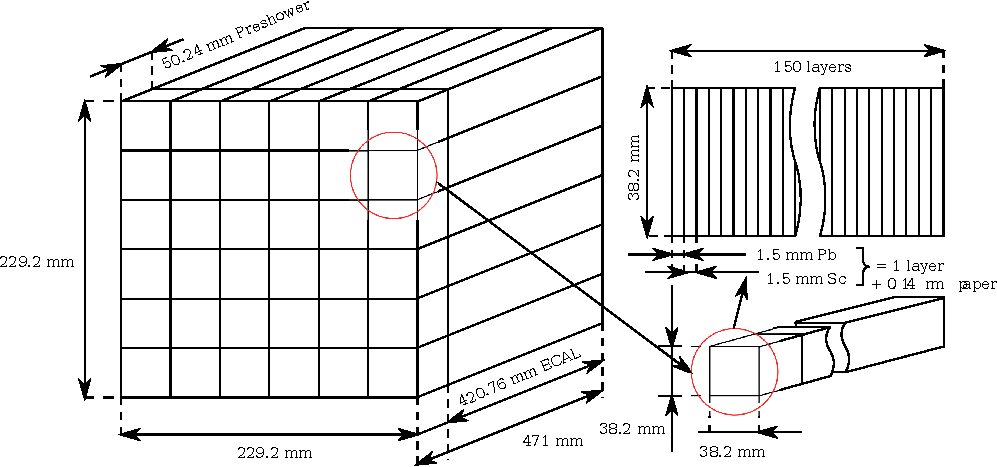
\includegraphics[width=\textwidth]{\pdirtwo/ECAL.pdf}
\caption[ECAL sketch]{Technical sketch of the Shaslik type calorimeter.}
\label{fig:ecal-sketch}
\end{figure}

\subsection{The Hadronic Calorimeter (HCAL)}
\label{ch2:sec:detectors-hcal}

The hadronic calorimeter in the NA64 experiment consist of four modules and its primary purpose is to stop and reconstruct the energy of a high penetrating particle. This includes the $\pi^-$ and $K^-$ contained as impurities in the beam but also neutrons and protons that can be produced in inelastic scattering in the ECAL. Additionally, although a complete stop of 100 GeV $\mu^-$ remains unfeasible, the HCAL can characterize very efficiently the presence of such particle after the ECAL, as the $\mu^-$ will leave the very distinctive MIP energy deposit inside each module, amounting roughly to $\sim 2.5$ \gev. Each module of the HCAL is a 3$\times$3 matrix of cells. Each cell is a sandwich of alternating layers of 25 \mmi Iron (Fe) and 4 \mmi of scintillating material separated by a 9 \mmi gap of air. Each cell consists of 48 such layers for a total thickness of $\simeq 7\lambda_{int}$. The lateral size of each module is 194$\times$192 \mms. The light readout is analogous to the one of the ECAL, using WLS-fibers embedded in round grooves in the scintillator plates. The fibers from each cell are collected together in a single optical connector at the side of the module. Each of the 9 optical connectors is then read-out by a single photomultiplier. Similar to the ECAL, these modules are calibrated using special runs where 50 \gev $\pi^-$ are shoot at different cells with the help of a mechanical table. The energy resolution estimated for this detector is $\sim 50\%/\sqrt{E[GeV]}$

\begin{figure}[bth!]
\centering
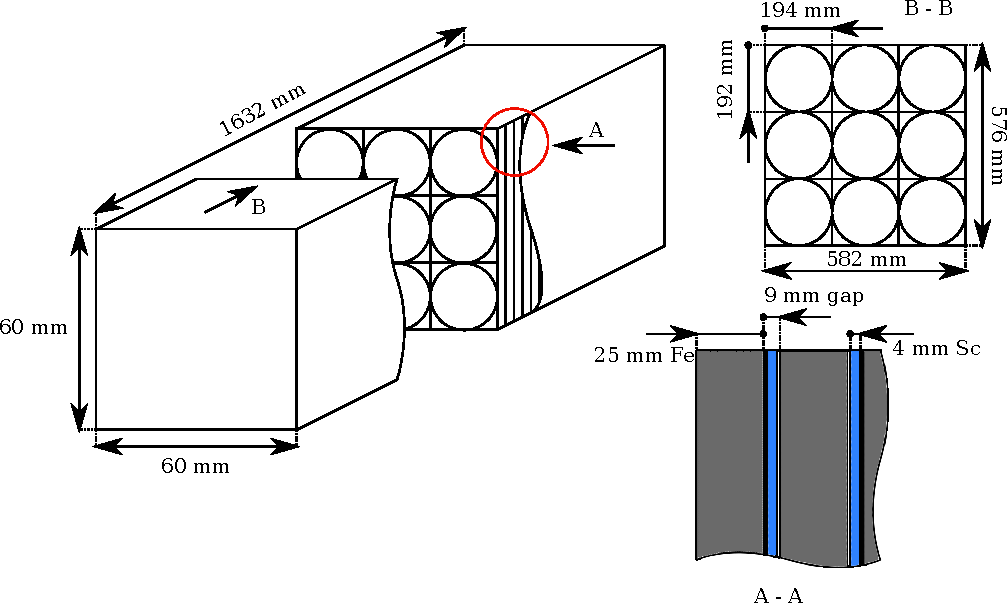
\includegraphics[width=\textwidth]{\pdirtwo/HCAL.pdf}
\caption[HCAL sketch]{Technical sketch of the HCAL module used in the NA64 experiment.}
\label{fig:hcal-sketch}
\end{figure}

\subsection{The Synchrotron radiation detector (SRD)}
\label{ch2:sec:detectors-srd}

The Synchrotron radiation detector (SRD) is a small calorimeter placed downstream in the arc described by the original beam axis and the bent beam. Its purpose is to measure the energy of the photon emitted by the passage of each electron in the magnetic field downstream. The energy range of such a signal is in the order of a few tens of MeV, hence the need for a larger precision compared to the calorimeter used to measure the primary beam. The detail of heavily charged particle suppression will be described more in detail in Sec.\ref{ch3:sec:bkg-srd}, here we described the detector technically.

Historically, the first Synchrotron radiation detector used was a set of 8 BGO crystals arranged in 2$\times$4 matrices placed parallel to the beam direction. Each crystal has a hexagonal shape with a diameter of 61 \mmi and a length of 200 \mmi. The light readout consists of an EMI PMT 9603 mount on the bottom of each crystal with optical grease. The BGO are excellent candidates for the SRD, due to the high light-yield and radiation length which coupled to their high Z makes them excellent gamma-absorbers \cite{bgo-crystal}. Indeed their rejection power can be as large as $10^{-4}$ and was demonstrated experimentally in the NA64 experiment (see Sec.\ref{ch3:sec:bkg-srd} for details). However, their large decay time of $\sim$300 \si{ns} creates a level of pileup that limit significantly their usefulness in a context where the intensity of the beam is very high.

The BGO detector was substituted with a shashlik type detector since the 2017 beam time. It is a shashlik type detector that uses three adjacent cells of dimension 60$\times$80 \mmi. Each cell consists of 100 layers with a lead-scintillator structure with dimensions 0.1 \mmi and 1.1 \mmi respectively. The light is read out by an R9420-100-10 Hamamatsu PMT with extended green spectral sensitivity \cite{hamamatsu-R9420-100-10}.

The time resolution for the shashlik type SRD is of $\sim$5 \si{ns}, which grants a suppressed pileup even at the largest intensity allowed in the H4 beamline.

\begin{figure}[bth!]
\centering
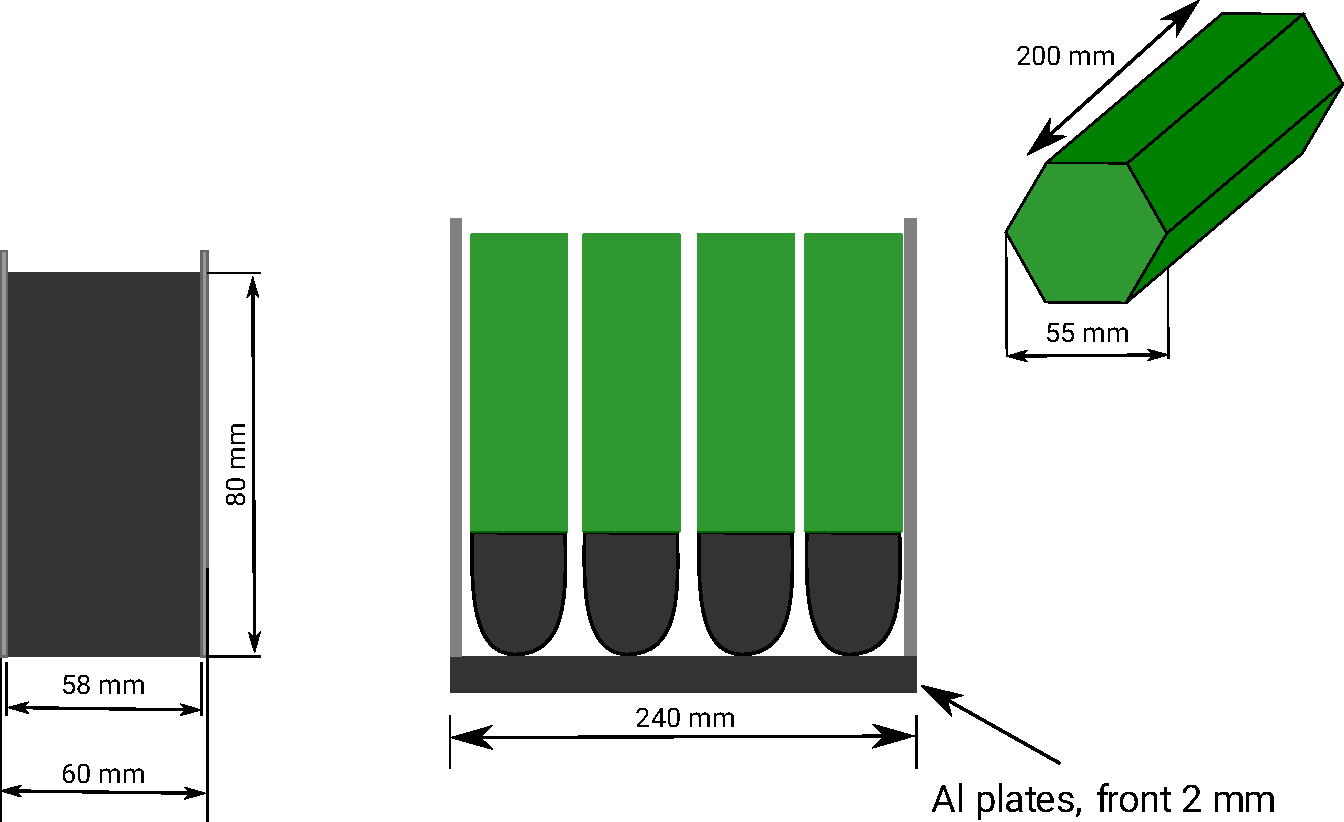
\includegraphics[width=\textwidth]{\pdirtwo/BGO.pdf}
\caption[BGO sketch]{Technical sketch of BGO crystal array.}
\label{fig:bgo-sketch}
\end{figure}

\begin{figure}[bth!]
\centering
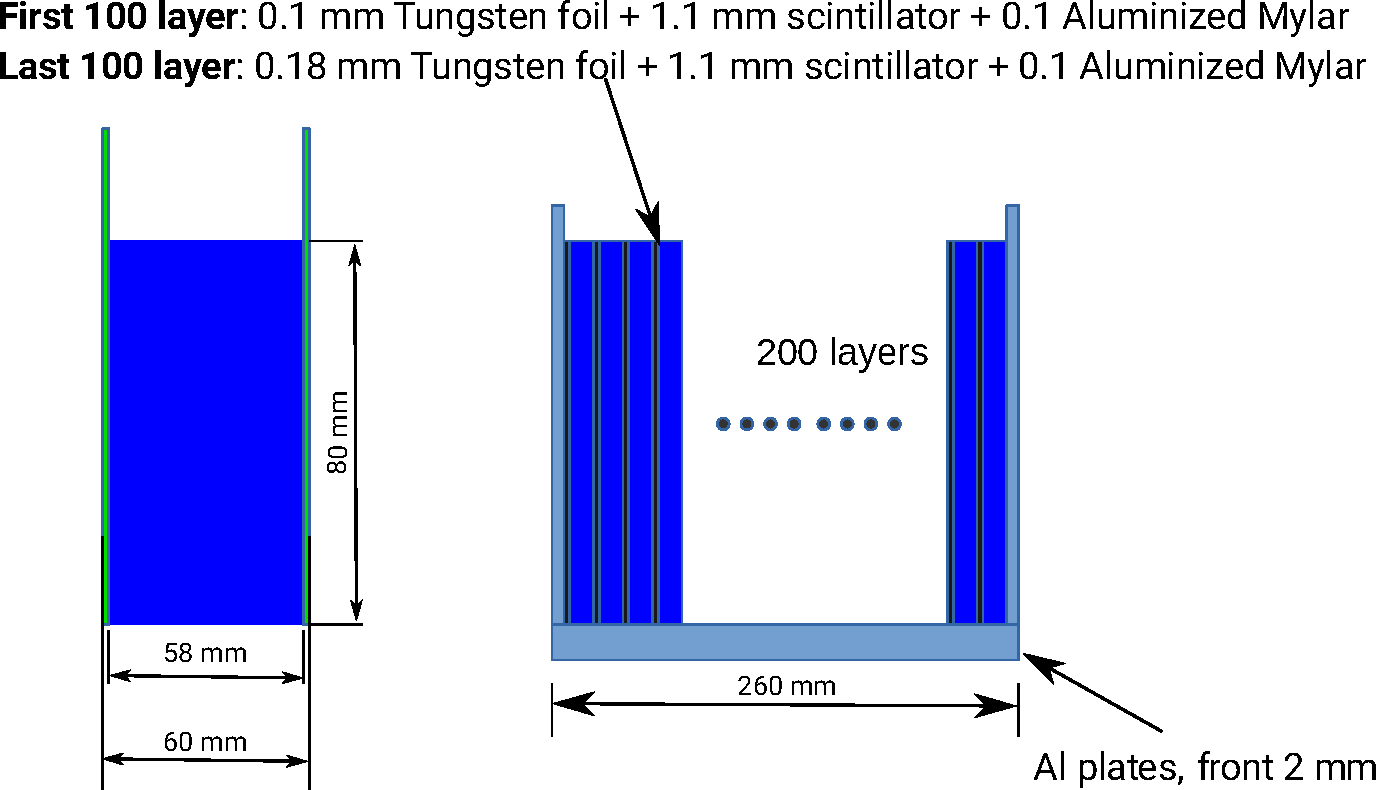
\includegraphics[width=\textwidth]{\pdirtwo/SRD.pdf}
\caption[SRD sketch]{Technical sketch of a single shashlik type module used in the NA64 experiment as SRD.}
\label{fig:srd-sketch}
\end{figure}

\subsection{The Veto system}
\label{ch2:sec:detectors-veto}

The Veto system is the set of detectors that has the purpose of measuring any particle penetrating one of the NA64 calorimeters to catch event with a long longitudinal shower profile that poses a risk to the hermeticity of the setup.

In general, a veto is a scintillator-counters of variable dimensions that are placed at the end of one of the calorimeter. The most relevant detector of this type is the VETO, a set of three scintillators mounted in series for a total dimension of 550$\times$550$\times$50 \mmc. The MIP inefficiency of this detector is estimated to be $\sim 10^{-3}$.

For the visible mode, it is crucial to maintain the dump as short as possible to increase the probability of the $\aee$ decay to be outside of the dump. For this purpose, the last layers of the WCAL sandwich are decoupled from the main readout and used as a veto (called W2). The dimensions of this counter are hence connected to the one of the WCAL: 23$\times$23$\times$6 \mmc. For testing purposes, a second thicker counter (called V2) is still placed at a distance of $\sim3$ \si{cm} from W2 to cross-check its inefficiency.

In general, a signal event in both visible and invisible mode need is characterized by the absence of energy in the veto counter placed behind that target dump. In practice, events with an energy deposit $<$0.8 MIP are accepted, taking into account both pedestal and energy resolution of these detectors.

\subsection{The Tracking system}
\label{ch2:sec:detectors-tracking}

The tracking system is the set of detectors that allows the full momentum reconstruction and track propagation in the NA64 setup. In the NA64 setup, four types of detectors are capable to reconstruct hits position: Micromegas (MM), Gas Electron Multiplier (GEM), Hodoscopes (H$_i$), and Straw chambers (St$_i$). While all of these detectors were useful for many different studies performed to analyze the beam composition and estimate the background, to this date only MM trackers are used as a direct part of the tracking system. This is to improve the overall efficiency of the selection criteria used for the momentum reconstruction and to limit the systematics of the experiment. In this thesis, however, a new analysis of the visible mode data is proposed that uses data from the GEM trackers to reconstruct the vertex position and the angles of the particles in the decay volume.

The exact working principle of each of these detectors is beyond the scope of this thesis. This section will be dedicated mostly to the description of the Micromegas detector, which was a direct part of every analysis currently performed and one of my main responsibilities during the whole thesis. More details on this detector in NA64 are found in \cite{pdegen-thesis}. In his work, he gives a very good overview of the working principle of the straw chamber and compares our modules to the MC prediction in the NA64 experiment.

\subsubsection{Micromegas}

Micromegas trackers are a set of eight Multiplexed XY Resistive Micromegas detectors (MM1-MM8) used to reconstruct the 2D hit position of the incoming particles in the NA64 experiment. The design and original testing of the first modules were already the topics of a previous thesis authored by Dipanwita Banerjee, which contains an excellent review of their working principle and characteristic \cite{dbanerjee-thesis}. For completeness, here we give a brief review of the detector. As shown in Fig.\ref{fig:mm-sketch}, the primary particle enters the gas box where it ionizes some secondary electrons. In NA64, the gas is a mixture of Argon (93\%) and C02(7\%). While Argon as noble gas is excellent to trigger the ionization, the C02 acts as a quencher to absorb UV-light emitted to avoid an excessive ionization that would both decrease the hit resolution and saturate the detector. The secondary electrons are then guided by the drift field in the amplification gap. The amplification gap is separated from the drift gap with a mesh formed by 400 wires with an aperture size of $\sim$45 \mum, wire diameter $\sim$18 \mum and thickness of the mesh of $\sim$ 29 \mum. The secondary electrons reaching the amplification gap experience an high electric field of $\sim$ 50 \si{\kilo\volt\per\centi\metre} which triggers a secondary avalanche that multiplies the electric charge. This charge is then collected in the strips of the PCB\footnote{Printed Circuit Board}. While the choice of the amplification field is typically set by the breakdown voltage of the gas, the choice of the drift voltage is not constraint, but a value too large can impact the transparency of the mesh. As pointed out in \cite{Bortfeldt:2014vvt}, an electric field of 0.6 \si{\kilo\volt\per\centi\metre} is a good rule of thumb to maximize the efficiency. Another problem for MM comes from the thin amplification region that makes them particularly vulnerable to sparks, which happens when the total number of electrons in the avalanche reaches the value of a few $\sim 10^7$, called Raether limit \cite{BAY2002162,BRESSAN1999321,Raether:102989}. Additionally to the damage the detector and the readout electronics, a spark can also lead to a dead time and thus to a significant reduction of its efficiency. The introduction of resistive strips, which add a continuous RC circuit on the top of the readout strip plane, leads to the spreading of charge and consequentially will counter spark development and the drop of voltage. These strips are grounded and separated from the readout strips via a thin insulating layer. The charge is therefore not directly collected by the cooper strips. Instead, an electrical signal is generated via capacitive coupling between the resistive and readout strips.

\begin{figure}[bth!]
  \centering
  %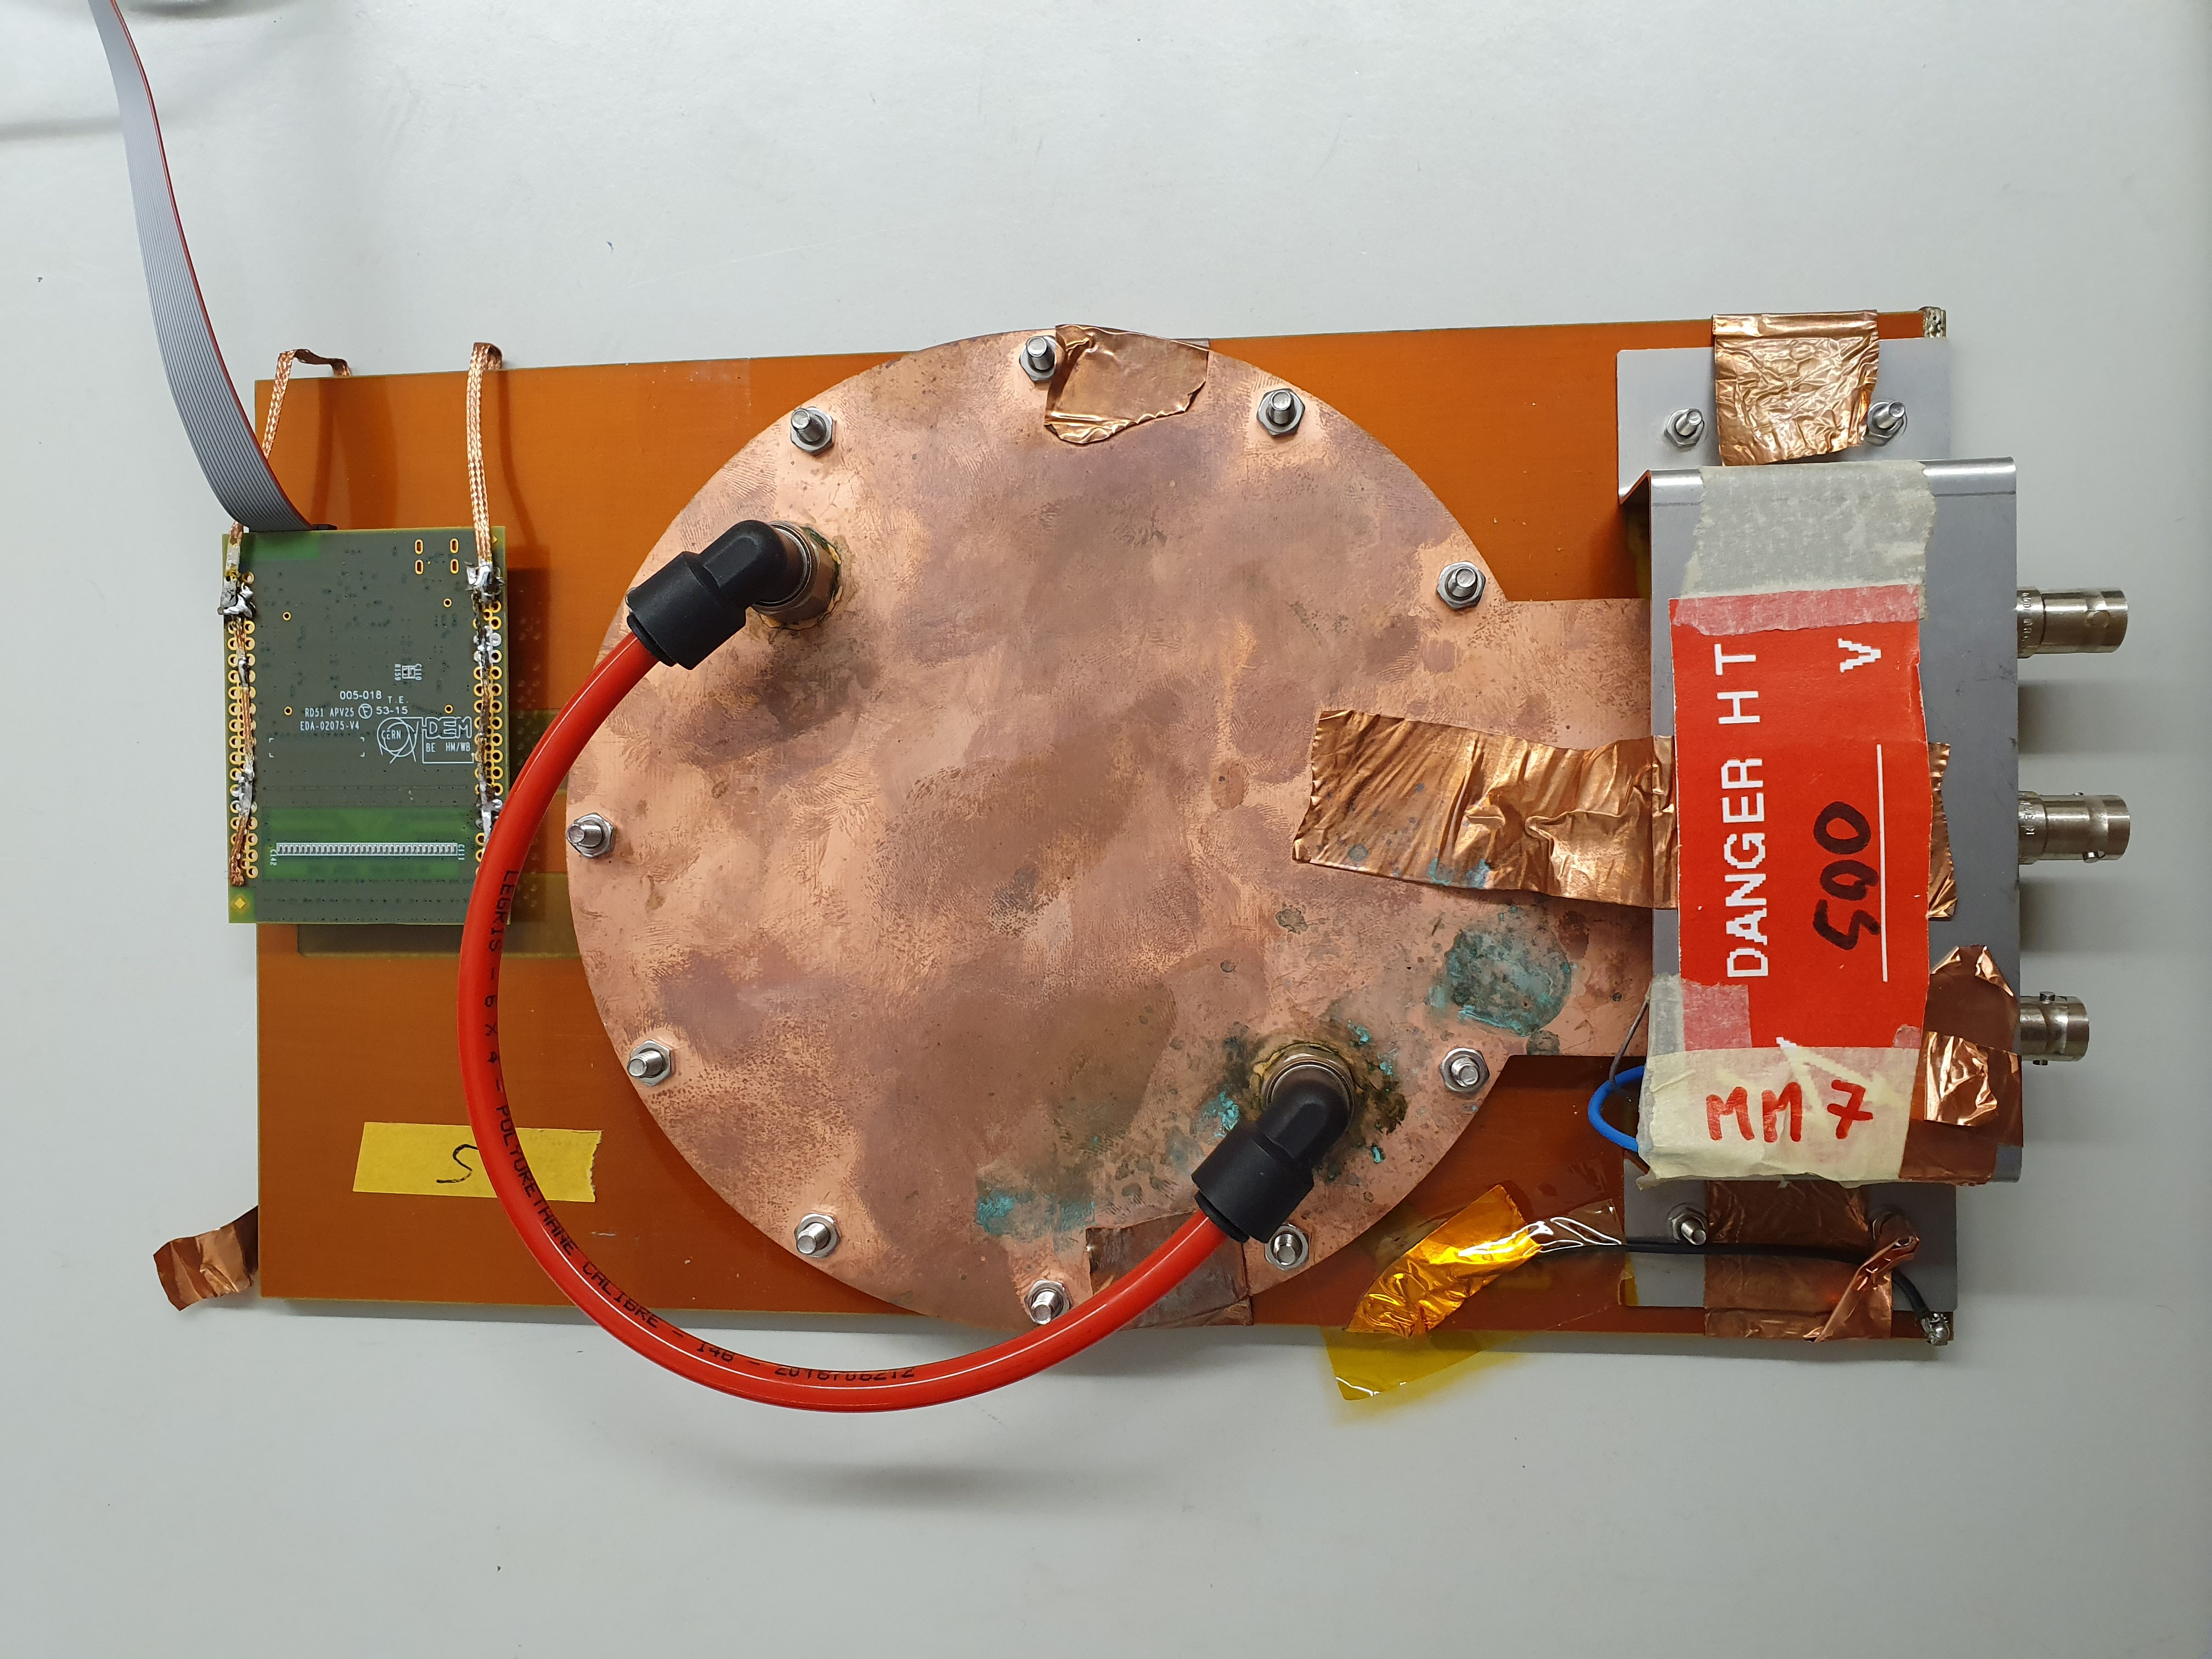
\includegraphics[width=\textwidth]{\pdirtwo/mm-photo-old.jpg}
  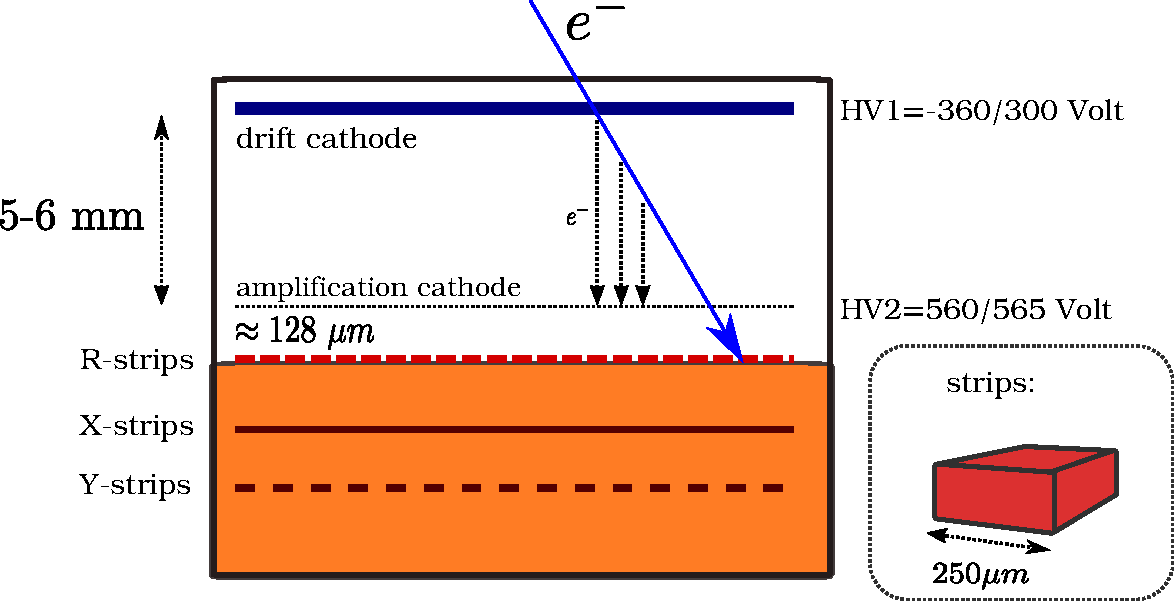
\includegraphics[width=\textwidth]{\pdirtwo/mm-principle.pdf}
\caption[Micromegas sketch]{Working principle and sketch of the Micromegas detector used in the NA64 experiment.}
\label{fig:mm-sketch}
\end{figure}

In the NA64 case, a negative voltage of 300-360 \si{\volt} (depending on the variable drift height) is applied to the drift plate. The mesh is connected to the ground while the resistive strips are kept at a positive voltage ranging from 560 and 565 \si{\volt} (due to some minor differences between MM). The resistive strips (R-strips) have a resistance of 1 \si{\mega\ohm} and are placed parallel to the X-strips. The Y-strips are placed after the R-strips and perpendicular to them. All set of strips have a pitch of 250 \mum, the width on the other hand is 200 \mum for the R and X strips and 50 \mum for the Y-strips.

Another important feature of this module is the genetic multiplexing of the strips: the strips of the micromegas detector are grouped in a set of five strips connected to a single channel. The results of this scheme are the reduction of the total number of channels needed for a complete readout of a module: the 640 strips of each micromegas (320 strips per plane) can be read by a single APV25 readout chip (see Sec.\ref{ch2:sec:daq}). The trivial consequence of multiplexing is a possible redundancy of the hit position of the incoming particle, which becomes more relevant as the occupancy of single events increases. To minimize this effect, one has to choose the mapping of this strip to maximize the separation between strips connected to the same channel, to make sure that no redundancy takes place. This technique was originally proposed in \cite{Procureur:2013yea}, and consist in distinguishing the original physical channel from the one created as an artifact by the multiplexing mapping by selecting as candidate clusters only the one where several (starting from a minimum of two) neighboring strips shows a signal over the decided threshold. An example of a single electron passing through a plane with different degrees of multiplexing can be seen in \ref{fig:multiplexing-example}. Producing the optimal mapping for the multiplexing where the redundancy is minimal is not a trivial task. Following the recipe in \cite{Procureur:2013yea}, one can produce an optimal mapping if the number of channels to map is a primary number. If we consider a detector with $n$ strips that are to be read by a number $p$ of channels, we construct $(p-1)/2$ sublists containing the channel numbers $p$ according to the formula:

\begin{equation}
\label{eq:mm-multiplexing-mapping}
1 + [(i \times s) mod p]
\end{equation}

where $s$ is the number of the sublists and $i$ is ranging from 0 to $p-1$. To complete the list, the channel can be used one more time in the end. In a more general case, Eq.\ref{eq:mm-multiplexing-mapping} can be used when the number of channels is not a prime number. In the NA64 case for example, where per plane we have a multiplexing factor of 5, and $n=320$, $p=64$ the sublists are still constructed following Eq.\ref{eq:mm-multiplexing-mapping}, but instead of using the number $s$ of the sublists a set of $(p-1)/2$ number $s_i$ is calculated to minimize the distance between neighboring strips mapped to the same channel $p$, where the set $s_i$ is typically produced using numerical methods. The map used for both planes of the 8 MM used in NA64 is presented in \ref{tab:mm-map-original}. A new improved map is being prepared for the next generation of the NA64 experiment as presented in Chapter \ref{chapter4}.

\begin{figure}[bth!]
  \centering
  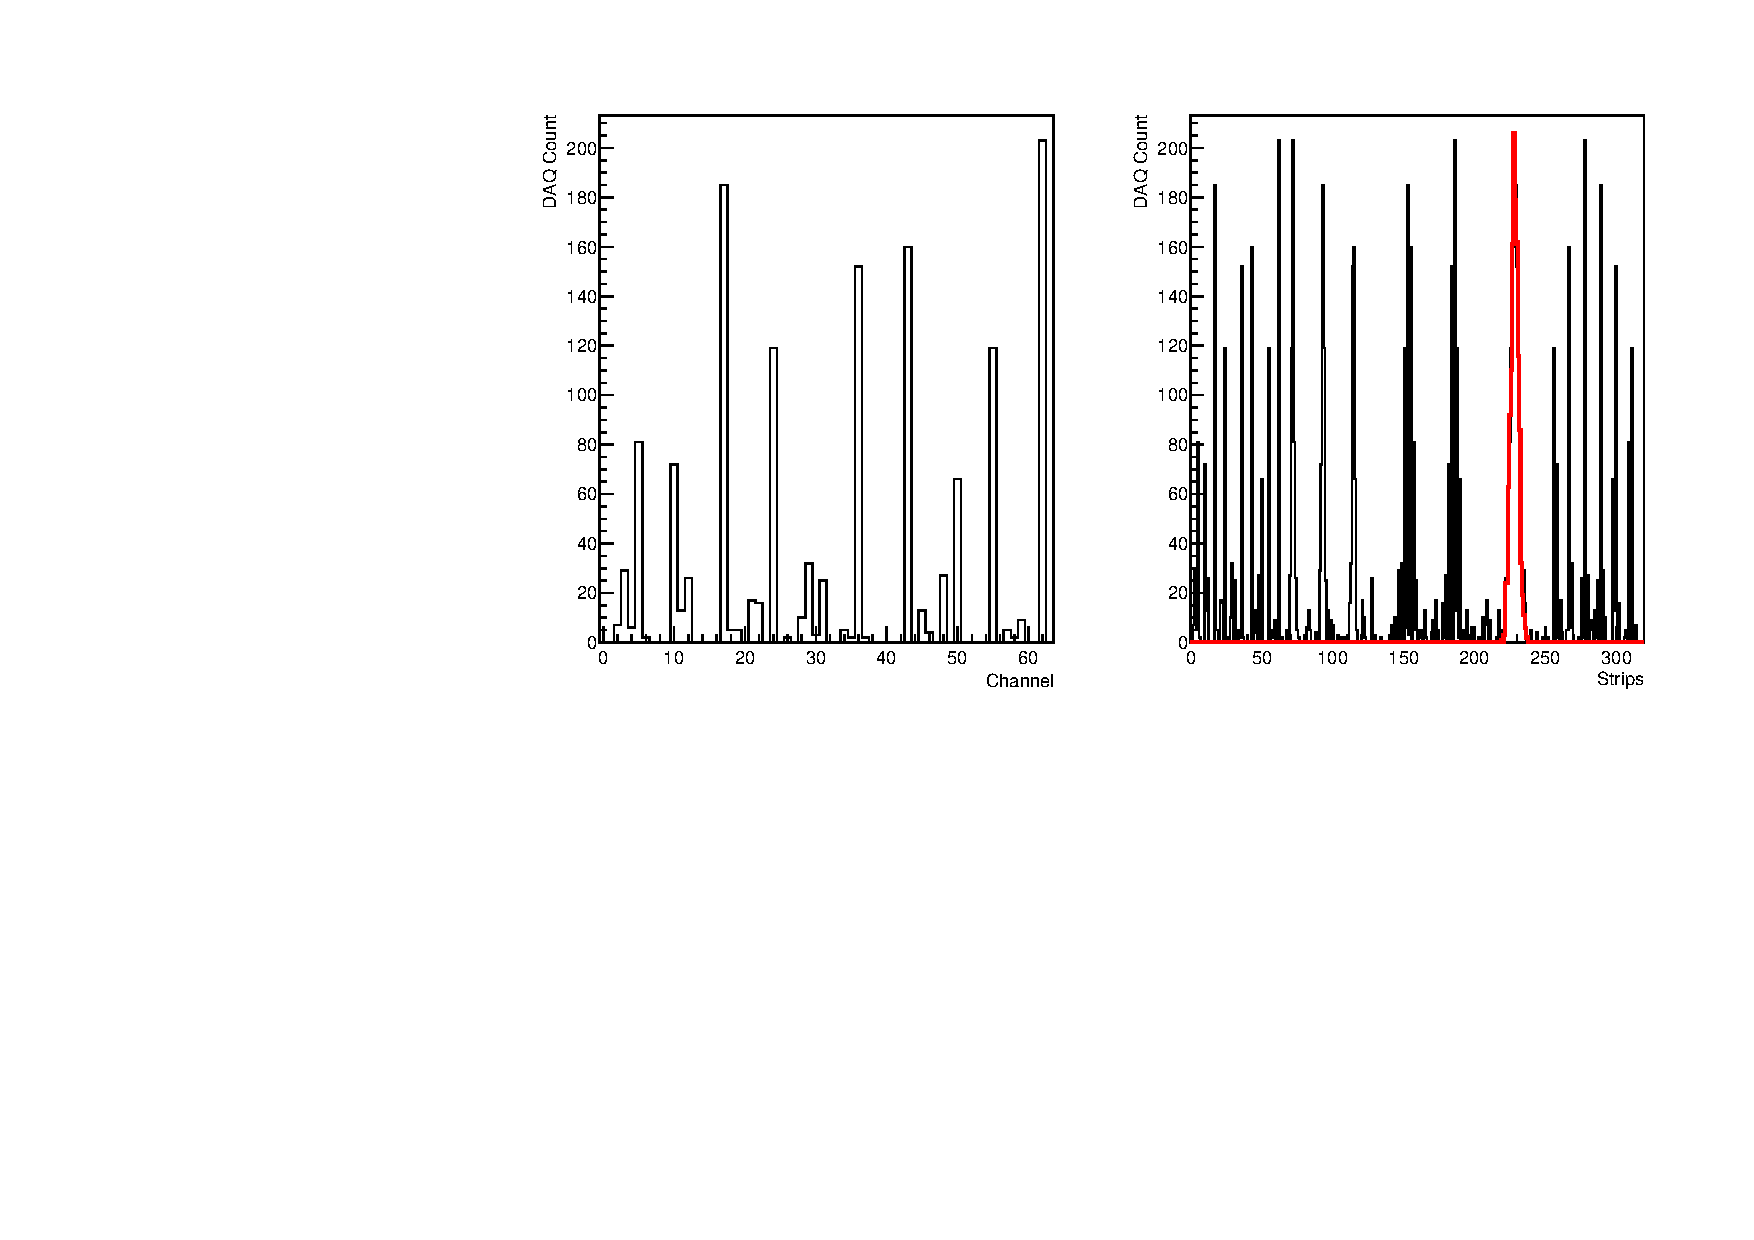
\includegraphics[width=\textwidth]{\pdirtwo/mm_output_example.pdf}
\caption[example of the readout of a multiplexing detector]{Left: example of the output in a Micromegas plane after the passage of a MIP. Right: same output transformed in the strips space using the multiplex map. The cluster selected by the reconstruction algorithm is shown in red.}
\label{fig:multiplexing-example}
\end{figure}

In NA64 the multiplexing feature is used for the first time in an experiment with an high-intensity. The results however show that these trackers are capable of resisting the high flux of particles and allow a precise momentum reconstruction with a precision of $\simeq$1\% at 100 \si{\gev} \cite{Banerjee:2017mdu}.

The total material budget for the two Micromegas, listed in Tab.\ref{tab:mm-mbudget} shows the amount of the material in the way of the beam.

\subsubsection{GEM detectors}
\label{ch2:sec:gem}
The Gas Electron Multiplier (GEM) is a gaseous tracking detector based on a similar principle of the Micromegas. Their performance is similar for both hit resolution, radiation hardness, material budget, and total active area. The working principle is described in detail in \cite{gem,SAULI20162,ABBON2007455}.

GEM consists of a composite grid of two metal layers separated by a thin insulator (typically Kapton) etched with a regular matrix of open channels. The two metal layers on the opposite side of the grid are kept at a suitable potential difference to create a large field in the hole. Secondary electrons are created by the primary during its passage in the gas and are amplified by the electric field during their drift through the holes. Electrons produced in this multiplication region are then collected by electrodes to measure the impact position of the original particle. To increase the signal GEM can stack multiple plates in series to increase the charge multiplication.

In NA64, the GEMs are produced stacking three consecutive foil to amplify the original signal of the secondary electrons. This allows the detector to reduce the voltage difference between foils to a minimum to ensure a low amount of discharge and allow them to operate efficiently ($\sim$99\% MIP efficiency) in the high intensity of the H4 beamline. The foil has an area of 100$\times$100 \mms with a hole pitch of 140 \mum. The readout consists of a two-layer strip anode with 256 strips per plane and a pitch of 400 \mum. Like the MM, the signal from each strip is processed by 128 channels APV chips, for a total of 4 chips to read out all strips for both XY plane.
One of the main differences between the two types of detectors is that GEM trackers are not multiplexed, meaning that every single strip is readout by a single electronic channel. For the momentum reconstruction, where only one primary particle hits the tracker in a single event, both MM and GEM detector performs similarly due to the multiplex map properties. When more then one particle hits the trackers, a multiplexed detector can create some redundancy that potentially limit the efficiency and bias the exact hit position. For this reason, GEM detector was placed inside the decay volume during the 2018 visible mode run to maximize the efficiency for signal events, where a $\ee$ is present inside the decay volume.

\subsection{The data Acquisition system (DAQ)}
\label{ch2:sec:daq}

The DAQ used for NA64 is a downscaled version of the COMPASS DAQ system \cite{Bodlak_2013,COMPASS-daq}. The detector's frontends are connected to the readout modules that with a processing speed up to 160 MB/s organize the digital information received by the frontends electronic into a preliminary event-like structure (sub-event building) (see Fig.\ref{fig:daq}. Triggers and control information are passed to these modules via the Trigger Control System (TCS), which work synchronously with the SPS duty cycle and creates the header and distributes the header containing the spill number, event number, and trigger type later used by the event builder PC. Two types of readout modules are used in NA64: the CATCH (Compass Accumulate Transfer and Cache Hardware), a general readout module that supports a wide range of frontend electronics, and the GeSiCa (Gem Silicon Control and Acquisition), which is optimized for the readout of the APV25 frontend chip that is used by both Micromegas and GEM detectors.

The APV25 is an ASIC that combines analog signals with a digital control \cite{Bodlak_2013} originally developed for the readout of the CMS silicon trackers \cite{article,inproceedings,apv-useguide}. Each of the 128 channels of the chip are made by a 60 \nas CR-CR shaping amplifier and a 192 samples deep analog pipelines. The amplifier integrates the current pulse from the input and output of a well-defined voltage pulse. A 192 samples deep analog pipeline is used to store the amplifier output to wait for the external trigger decision. This pipeline is made of switched-capacitor elements. 160 of the 192 memory cells are organized in a ring buffer with a write and trigger pointer. The distance between the two defines the trigger latency which is a configurable parameter. When one of the pipeline columns is flagged for readout, it is copied into one of the remaining 32 memory elements, organized like a FIFO \footnote{\textbf{F}irst \textbf{I}n \textbf{F}irst \textbf{O}ut is a form of data buffer that conserves the order of the incoming data.}. The data are stored here until are sent out by the multiplexer. From here, the data is sent to an ADC\footnote{\textbf{A}nalog to \textbf{D}igital \textbf{C}onverter} modules (which can accommodate up to 4 APV chip) that digitizes the pulse before sending it to the GeSiCa. The ADC has two possible modes of operation, the latch-all mode, and the sparse mode. When using the latch-all mode, the signal amplitudes of all channels is sampled three times with a clock cycle of 25 \nas and transmitted to the GeSiCa. In this mode the trigger rate cannot be higher than $\sim$1 \si{\kilo\hertz} due to the large amount of data received by the APV25. To reach higher trigger rates, the sparse mode is used instead. When in sparse mode, only channels with amplitudes above a certain threshold are sent to the GeSica by the ADC module. This allows us to increase the manageable trigger rate to $\sim$10 \si{\kilo\hertz}. In NA64, the latch-all mode is used to record the data coming by the APV25 connected to the trackers but in absence of the beam. This procedure is repeated every $\sim$10-15 run approximately to record the pedestal of each channel. The pedestal recorded are then used to set the threshold (2$\sigma$ for MM and 3$\sigma$ for GEMs) for the sparse mode, which is used during data taking to maximize the trigger rate.

\begin{figure}[tbh!]
\centering
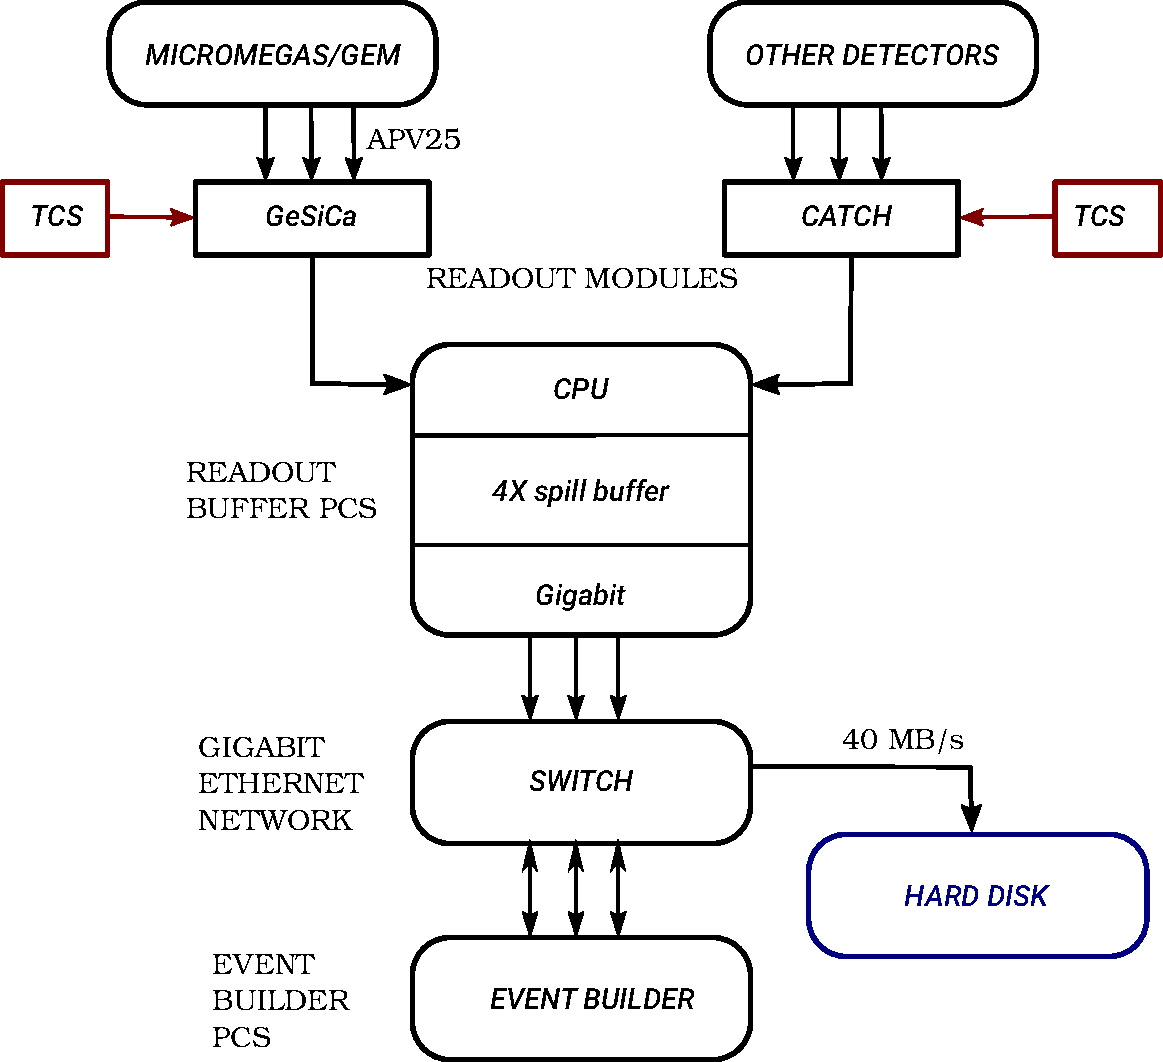
\includegraphics[width=\textwidth]{\pdirtwo/daq.pdf}
\caption{Scheme for the NA64 DAQ}
\label{fig:daq}
\end{figure}

During the calibration procedure, the three samples received by each channel of the APV25 are also used to set the latency of the trigger. The latency of the trigger is optimal when it covers precisely the rising edge of the pulse received by each channel of the APV25. If we define a$_0$, a$_1$ and a$_2$ as the three samples recorded in consecutive order by a single APV25 pipeline, the latency is to be set such that the second sample a$_1$ is larger than the other two amplitudes. This can be best summarized in the so-called "banana plot" of Fig.\ref{fig:banana-plot}, which is a heat map plotting the frequency of events with certain pulse structure. The sampling of the pulse shape also provides additional information about the time of arrival of the primary electron. By reconstructing the pulse shape rise time one can improve the time estimate by the usual 25 \nas (limited by the clock frequency of the APV) down to $\sim$15 \nas \cite{Banerjee:2017mdu}. To achieve this, the pulse is described by the following function:

\begin{equation}
\label{eq:apv-pulse}
r(t) = \frac{r_0}{(1 + \exp{\frac{t-t_0}{\tau}})}
\end{equation}

Where the parameters $r_0$, $t_0$ and $\tau$ are fitted using the same data measured at different values of the latency. The time of arrival is then extracted by reversing the function and solving for $t$ as a function of the ratio between pulses:

\begin{equation}
\label{eq:2}
t(r) = t_0 + \tau \times \ln{\frac{r_0}{r} - 1}
\end{equation}

A complete description of the method that takes into account the errors of the ratio and the parameters is described in \cite{dbanerjee-thesis}.

\begin{figure}[!bth]
  \centering
  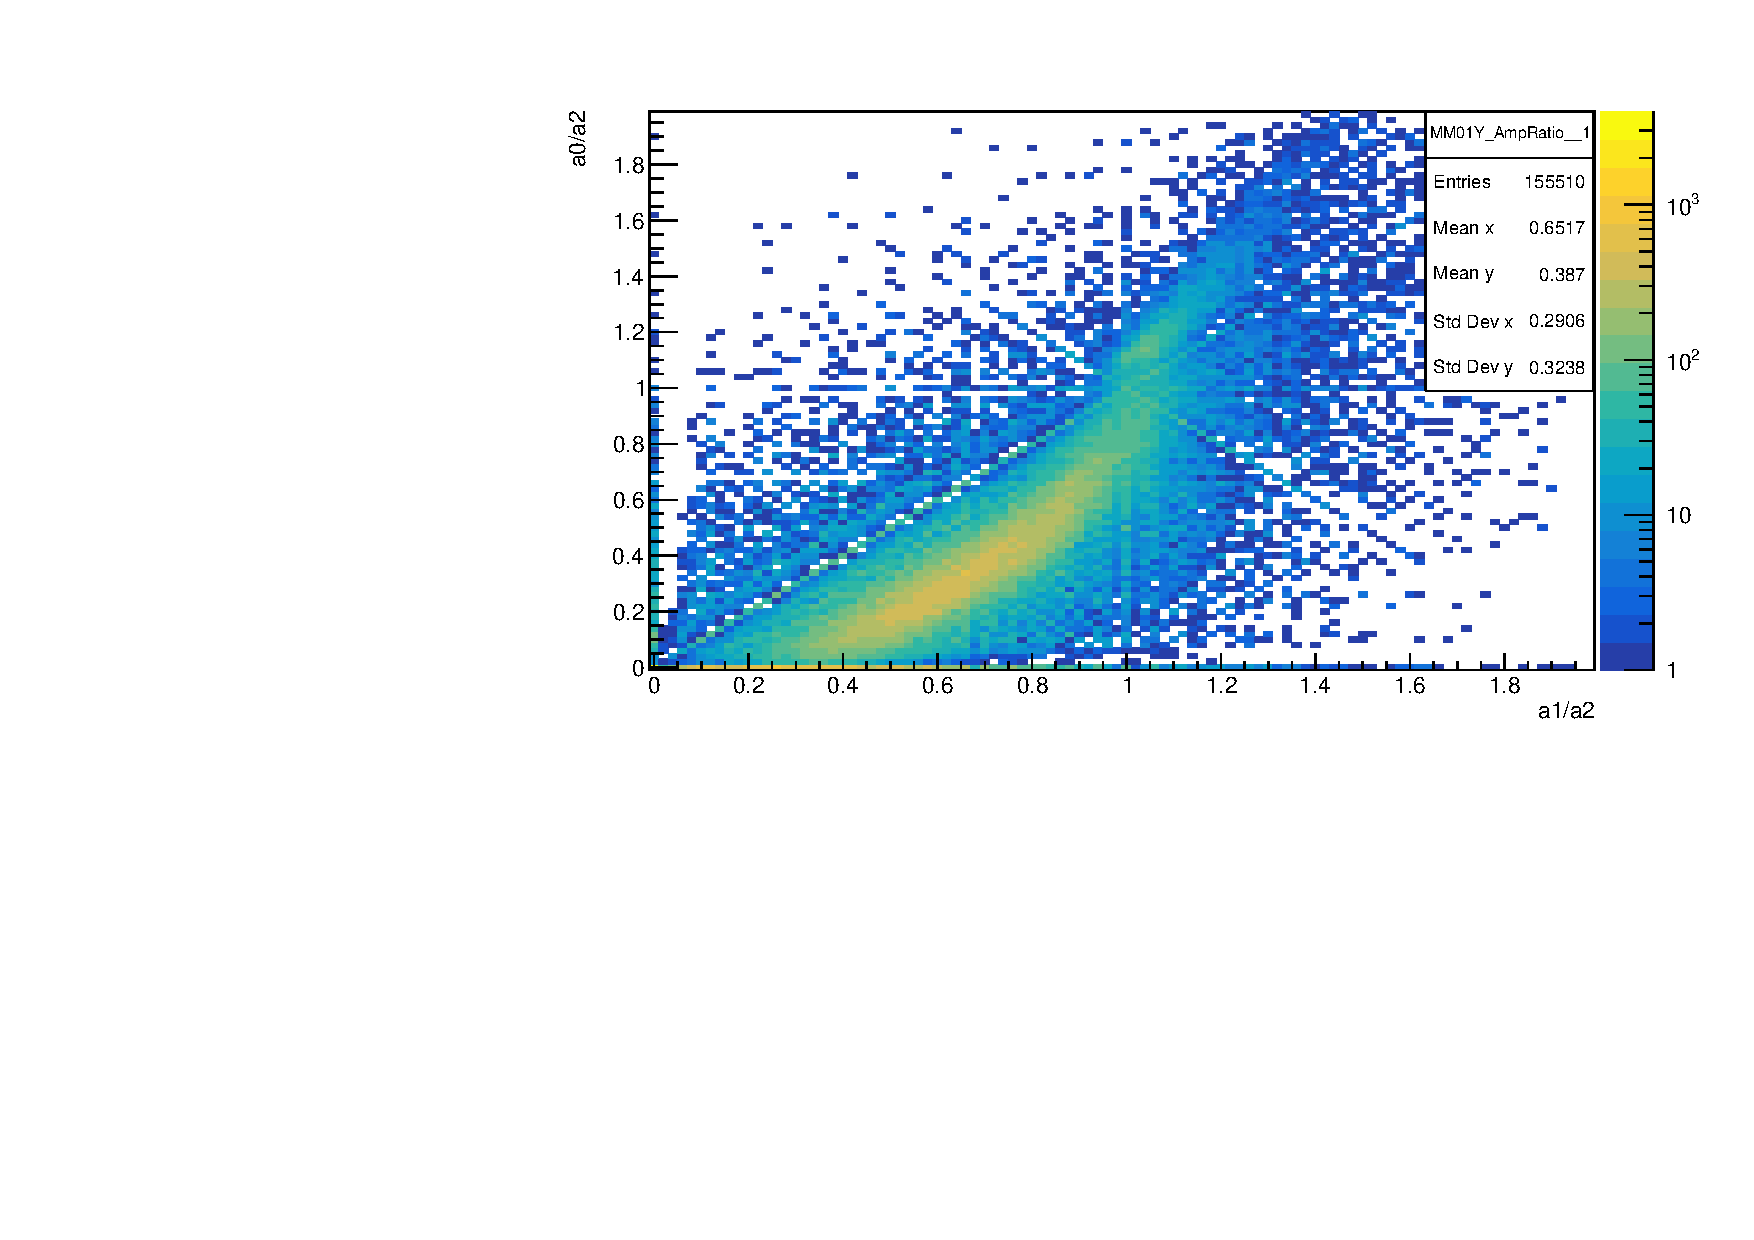
\includegraphics[width=\textwidth]{\pdirtwo/MM1Y_bp.pdf}
\caption[APV25 banana plot]{Ratio between the first two vs the last two amplitudes sampled in an APV25 chip after the proper latency is set for the chip. The typical "banana" shape of this plot is the sign that the pulse is sampled during its rising edge.}
\label{fig:banana-plot}
\end{figure}

After passing through the ADC, the data is sent to GeSica using a high-speed optical cable. The Gesica can accommodate up to 4 ADC (for a total of 16 APV chips) and has the purpose of multiplexing the incoming data stream, merging the header information from the TCS\footnote{Trigger Control System} with the corresponding data coming from the APV, and finally putting the event data block into the S-link format. Finally, the information are transferred to a high-performance readout buffer PCs (ROB) via the S-link protocol \footnote{The S-link is a protocol developed at CERN for fast point to point connections, typically between front-end electronics and the readout electronics \cite{s-link}.}. In the NA64 case, to accommodate the many GeSica and CATCH modules used, and S-link multiplexer is used to combine multiple modules before sending the data to the ROB. As seen in Fig.\ref{fig:daq}, the Readout buffer PCs receive the information from the multiplexer and stores them in four different spill buffer \footnote{A spill is a 512 MB SDRAM module which can store the data of at least one spill \cite{COMPASS-daq}}. A Gigabit Ethernet\footnote{Gigabit Ethernet is a standard developed by the Institute of Electrical and Electronics Engineers(IEEE) and Local Area Networks (LANs).} switch connects the ROB with the event builders PC. Here the data of every single event and merges them into a single event data block using the event identifier provided by the TCS receiver. After this process, the event is ready to be recorded to the long term storage, in this case of 5 TB SATA Hard Disk with a speed of 40 MB/s. Thanks to this design the DAQ takes advantage of the beam structure of the H4, characterized by a high intensity for 4.8 \si{\second} where the spill buffers are filled by the information coming from the readout modules followed by a long recovery time of $\sim$20 \si{\second} that are used for the event building and to write all the information to the tape.

%%% Local Variables:
%%% mode: latex
%%% TeX-master: "../PhDthesis"
%%% End:
 
% Chapter 3

% variables
\newcommand{\pdirthree}{chapters/plots/chapter3}

\chapter{Data analysis} % Main chapter title
\label{chapter3} % For referencing the chapter elsewhere, use \ref{Chapter1} 

% ----------------------------------------------------------------------------------------

In the previous chapter, we explored the general concepts, and all the components characterizing the invisible and visible mode setup. In this one, we will described the method used to analyze them. In Sec.\ref{ch3:sec:analysis-approach}, I will give an overall explanation of the analysis approach of NA64 with a flowchart to explain each step. After that, a description of the simulation framework of NA64 will be provided in Sec.\ref{ch3:sec:geant4}, this is the main tool used for prediction of both background and signal rate.
A detailed description of two background rejection tools developed as direct consequence of my work, namely SRD rejection and shower profile analysis, will be given in Sec.\ref{ch3:sec:bkg-srd}-\ref{ch3:sec:bkg-ecal-profile}. After that, in Sec.\ref{ch3:sec:dimuons}, we will show how the rare interaction $\emu$ is used in NA64 as an important tool to validate the MC and correct the signal yield for systematic effects.
Finally, we will provide a description of both analyses performed for the invisible and visible mode setup in Sec.\ref{ch3:sec:analysis-invis} and Sec.\ref{ch3:sec:analysis-vis} respectively. In the case of the visible mode, this section also includes a new analysis I performed which uses the information recorded by the trackers on top of the one of the calorimeters.
The list of the selection criteria is provided, and the background is discussed in detailed. We show that in both modes the background is expected to be under control, with an average of expected event in the signal region of $\simeq 0.5$ for the invisible mode and $\simeq 0.01$ for the visible mode.


\section{General Analysis approach}
\label{ch3:sec:analysis-approach}

To define the analysis method the choice of signal region and the selection criteria are crucial, which means deciding what are the characteristics that define an event where an $\DM$ is produced. The figure of merit is to maximize the sensitivity of the experiment. In other words, if $\DM$ does exist, one wants to produce an analysis that maximizes the probability of discovering it, and otherwise minimizes the probability of producing a false positive. In these type of experiment the number of events in the signal region is counted and compared to the expected background calculated beforehand. Assuming the signal rate constant and the probability of each event to be independent from the last measured, the number of events in the signal region will follow a Poisson distribution. We can, therefore, express the number of events expected in the signal region $N_{SR}$ according to the following distribution:


\begin{equation}
  \label{eq:poisson-simple}
  N_{SR} = \frac{(\mu s + b)^ne^{-(\mu s + b)}}{n!}
\end{equation}

where $s$ and $b$ represents the expected number of events for signal and background in the signal region, and $\mu$ is a control parameter that describes if the signal is present. If the signal is properly modeled, the parameter $\mu$ can be either 0 (no signal present) or 1 (signal is there), but we can also choose to allow a continuous spectrum of $\mu$, which means that the signal can have a larger (or smaller) rate than anticipated. The experiment will claim a signal if the number of events found exceeds the expected background $b$ to a degree that $\mu = 0$ is no longer compatible with the data. The current standard for discovery in the HEP\footnote{High Energy Physics.} community is the 5$\sigma$, which means that the number of the events is larger than the one predicted by the $\mu = 0$ hypothesis by 5 standard deviations\footnote{This is to be intended as correspondent p-value in a Gaussian distribution. The actual distribution defining the number of events observed is arbitrary and typically computed using numerical methods.}. The probability of an experiment returning such an outcome when no signal exists can be calculated to be 2.87$\times$10$^{-7}$.

If no signal is observed, a second problem arises, how do we interpret this result? In principle, since the initial no-signal hypothesis (frequently called $H_0$) remains satisfactory to explain the data, the hypothesis implying the existence of new physics is not needed (frequently called $H_1$). However, there might be a minimal difference between the two, so the fact that $H_0$ is sufficient to describe the data does not mean that $H_1$ is wrong, just that our experiment is not sensitive enough to distinguish between the two. After accumulating a sufficient number of EOTs, the difference in the prediction between the two hypotheses will be significant, such that one of the two can be rejected as insufficient to properly describe the data. The standard to reject an hypothesis is less stringent than the one used to claim a discovery. The exact standard differs between different searches, in the case of the dark photon $\DM$, the significance is set to be 90\% \cite{battaglieri2017cosmic}. We define $CL_{s+b}$ the "confidence level" as the probability to observe a number of events larger than the one observed in the experiment given the signal hypothesis to be true (hence $\mu = 1$):

\begin{equation}
  \label{eq:confidence-level-poisson}
  CL_{s+b} = e^{-(s+b)}\sum^{n_{obs}}_{n=0} \frac{(s+b)^n}{n!}
\end{equation}

In the NA64 experiment, we can assume that no background is expected in the signal box. Hence, if the signal hypothesis is wrong, we expect to observe zero events in the signal region during a run of our experiment. We take $n_{obs} = 0$ and $CL_{s+b} = 0.1$ and we solve the equation for $s$. The number $s$ of expected $\DM$ events for an hypothesis to be rejected is 2.3 events.

After we finish the analysis of the data, if no event is in the signal region, we can reject all the hypothesis $H(m_{\DM}, \epsilon)$ that predict a number of signal events larger than 2.3. There are of course some complications to this: the background $b$ is often not exactly zero, which means in the more general case one has to numerically solve the equation above for $s$. A more detailed explanation is given in Appendix.\ref{AppendixE}.

For a complete analysis, we need to calculate the expected signal s, the expected background b, and properly take all uncertainties into account. In first approximation, we developed equations that can be used to compute the signal rate back in Sec.\ref{ch1:sec:dm-u1model}. However, each of the selection criteria used to reject the background will reduce the signal efficiency and needs to be taken into account. Estimating the background is also typically challenging, it is enough to take a look at all the possibly decays of the $K^-$\cite{particle-strange-mesons} to see how many effect could in principle cause the disappearance of a fraction of the total initial energy.

A precise knowledge of the experimental conditions is needed to properly define the expected signal $s$ and the expected background $b$ for a given hypothesis of dark matter $\dmhypo$. We need first of all a tool that can reproduce precisely not only the single particles under analysis but also their interaction with the setup and how each detector responds to these interactions. Indeed while Eq.\ref{eq:dm-rate} is a good starting point it hardly represents all the possible outcomes of a particle entering the NA64 setup.
%For example if the $\DM$ is not produced in the first layer how we assumed but instead after a few radiation length the energy spectrum will be different from the one we approximated initially. This can especially have a significant effect after the selection criteria are applied to the sample considered. An accurate description is even more important for background, usually caused by the tail of very complicated distributions, hard to characterize starting from simple equations.
%Sometimes even unexpected effects can play a role. An example of this will be given in Sec.\ref{ch3:sec:bkg-srd}: if we calculate the contamination of hadrons after a synchrotron radiation cut, we might be tempted to say that this type of particle is suppressed with the fourth power of its mass since the mean power emitted is $P \sim 1/m^4$. However, as we will see, hadrons can ionize electrons during their travel in the vacuum tube, which can in turn posses energy of several tens of MeV in some fringe cases, effectively mimicking the signal of Synchrotron Radiation! From an initial suppression factor estimated to be of $\sim 10^{-8}$, we now have just $\sim 10^{-3}$, this is more than 5 order of magnitudes difference from our first naive estimate.\footnote{We will see in Sec.\ref{ch3:sec:bkg-srd} that the suppression factor can be improved by exploiting the segmentation of our detectors.}

To compute these effects more precisely, we use a Monte Carlo simulation based on the Geant4 software \cite{AGOSTINELLI2003250,1610988} developed at CERN. This approach is very useful to directly simulate the background of the experiment, but it has some shortcomings. The simulation is a computationally expensive task: a single event requires $\simeq$1 second to be simulated by a single CPU\footnote{The exact time depends on what particle is exactly simulated. For example, the simulation is $\simeq$60 faster for muons.}. Thus, even with the help of a very large cluster like the one provided by the CERN computing infrastructure, more than $10^8$ EOT are challenging to simulate. This is still a long way from the $\sim 10^{11}$ EOT accumulated at the present date. To solve this, some type of background, like event with dimuon production $\emu$, electronuclear interactions, and the decay of the $K^0_S$, are accounted using dedicated simulation with biased cross-section/branching ratio (see Appendix.\ref{appC:sec:physics-list}). This allows us to study the background at a level compatible with the EOT accumulated in our search.

Because of the different physics involving them, it is instructive to divide the background by the primary particle considered. We define three categories:

\begin{description}[leftmargin=!,labelwidth=\widthof{\bfseries Electronic background}]
\item[Hadronic background] Background coming from a hadronic ($\pi^-$,$K^-$,...) primary.
\item[Muonic background] Background coming from a $\mu^-$ primary.
\item[Electronic background] Background coming from a $e^-$ primary.
\end{description}

This classification is convenient if one wants to study the background using MC-simulations. However, there is some overlap in the physics of these three scenarios. A trivial example would be the decay $\pi^- \rightarrow \mu^-\nu$, where an initial $\pi^-$ produces a $\mu^-$ in our setup. A more relevant but involved example is an $e^-$ or a $\gamma$ which triggers an hadronic shower after an inelastic scattering with a nucleus. This can cause energy escaping in the form of hadron, and since the initial particle is an electron, such background is also accepted by the SRD criteria. The main advantage of this classification is that it let us calculate the suppression factor for the background with a simple argument without necessarily using the MC-simulation. For example, for both hadronic and muonic background, we can conservatively assume a factor $10^{-5}$ of suppression due to both the beam-composition ($\lesssim 10^{-2}$) and the SRD selection applied upstream ($\lesssim 10^{-3}$). A specific list of all background considered for both searches is provided in Sec.\ref{ch3:sec:bkg:inv} for the invisible mode and Sec.\ref{ch3:sec:bkg:vis} for the visible mode.

Next we need to improve the simulation to properly reproduce the data. Indeed while Geant4 simulates reliably particle interaction inside materials, by default no particular detector response is assumed. This has several consequences, the most important of which is that the detectors resolution is not properly reproduced. We can extract the energy deposited inside the ECAL or the position where the incoming particles hit a Micromegas detector, but none of these quantities will be measured with absolute precision in our real experiment. To improve the reliability of the MC, an approach relying on data collected in the calibration run is used. The Data collected in the electron/hadron calibration runs are used to directly measure the detector response, and this information is used to improve the distributions produced by the simulation. In this thesis, we will refer to this process as \textbf{Digitization}.

After that, selection criteria are set to maximize the sensitivity of the experiment. This is done by simulating $\DM$ (or other types of Dark Matter) inside our setup and comparing their signature to the leading background in one of the relevant distribution (for example the synchrotron radiation detected in the SRD). We then choose the cut where the significance, defined as $S = s/\sqrt{s+b}$, is maximized.
%In some cases, where two distributions happen to be correlated (for example the SRD energy deposit and the $\chi^2$ compatibility of the signal shape with an e.m.-shower in the ECAL), the selection criteria are optimized using the 2D-distribution of the two variables instead.

We then start the comparison with the data collected with the physical trigger. This is tricky, because it implies the risk of substantial bias, but is necessary to study possible systematics that are still not correctly reproduced. One example of this would be the physical trigger described in Sec.\ref{ch2:sec:detectors-trigger}, that is a source of uncertainty for the signal yield. To solve this issue, NA64 uses a Hidden Signal Box blind analysis\cite{blind-analysis}: a small portion of the data ($\sim$10\%) is used to study in detail the distribution observed after the physical trigger while the signal box remains hidden until the final analysis involving the full sample is performed. This method allows to study more in detail distributions that might affect the background by directly looking at the data without introducing too much bias in the procedure. An example of this is the large-angle scattering of hadrons, that causes the energy to escape the setup transversely, and is estimated using data-driven methods. Since the knowledge of the background improves after this step, some corrections to the selection criteria are applied to further increase the sensitivity.

One also wants to estimate properly the efficiency of signal detection, including possible fluctuation in the efficiency of the DAQ or the physical trigger. Hence, a class of events that has similar properties to the signal is very desirable to study in detail the properties of a signal-like event and how are effected in by our measurement method. It is not obvious that such a class exists, but turns out the NA64 experiment is lucky! The dimuon production starting from gamma $\emu$ shares an important number of properties with the signal and at the same time can be easily distinguished from it by looking at the energy deposited in the HCAL: a double-MIP signature in each module. Additionally, being a QED interaction, it can be reproduced reliably by the simulation , hence the difference between the expected number of dimuon and the observed number of dimuon can be used to weight each run. This way, the systematics of the trigger and the setup are accounted for, even if they evolve with time. To each run is assigned a weight taking into account the dimuon discrepancy mentioned above $\omega_i = N^{data}_{dimu}/N^{simu}_{dimu}$, and the total number of effective EOT is obtained:

\begin{equation}
  \label{eq:effective-eots}
  N_{eff}^{EOT} = \sum_{i=run number} \omega_i \cdot N^{EOT}_i
\end{equation}

After this stage, we are finally ready to unblind the data and proceed to the final analysis. We now count the events in the signal box after the selection criteria are applied to the full sample, and we compare this number to the expected background. 

In all analysis performed by NA64 to date \cite{Banerjee:2020fue,Banerjee:2019hmi,NA64:2019imj,na64-prd,Banerjee:2018vgk,Banerjee:2016tad} no signal event was found in the signal box. To cast our results, a confidence limit was calculated using the modified frequentist approach, taking the profile likelihood as test statistics\cite{JUNK1999435,Read_2002,Cowan:2010js}. Compared to Eq.\ref{eq:poisson-simple}, here we consider all sources of background calculated and we take them into account. The expected signal for each hypothesis $\dmhypo$ is calculated using the following equation:

\begin{equation}
  \label{eq:dm-expected-signal}
  N^{tot}_{\DM} = \sum_{i=runs} n_{\DM}(m_{\DM},\epsilon) \times \varepsilon_i(m_{A'},\epsilon) \times N^{EOT}_i
\end{equation}

Where $n_{\DM}(m_{A'},\epsilon)$ is the rate at which $\DM$ is produced considering the efficiency due to the selection criteria, $\varepsilon_i(m_{A'},\epsilon)$ is an efficiency factor taking into account detector inefficiencies and other sistematics\footnote{Not to be confused with the kinematic mixing $\epsilon$}, and $N^{EOT}_i$ is the number of collected EOT in the run $i$.

A summary of the full analysis machinery is depicted in Fig.\ref{fig:analysis-chart}. In short, we characterize the following steps:

\begin{enumerate}
\item A MC-simulation based on a Geant4 code is used to create all the distributions relevant for the experiment.
\item Each event produced by the simulation is used as input by a reconstruction algorithm that adds detector effects and produces artificial data in a format equivalent to the data.
\item Using the artificial data, selection criteria are chosen in each detector to maximize the significance of each cut. An estimate of the background is produced by dedicated studies based on the MC-simulation.
\item A sample of the data ($\sim$ 10\%), is used to test the selection criteria chosen. Modifications to the selection criteria are applied to correct for unforeseen effects observed in the data. The background estimate is improved using data-driven methods. The signal region remains blinded following the principle of Hidden signal box blind analysis.
\item Artificial samples of signal events are created using different signal hypothesis $\dmhypo$. The signal yield for each of them is calculated by running all selection criteria using the same analysis program used for the data. The expected rate is also corrected taking into account detector efficiency and other systematic effects using a dimuon sample as a benchmark.  
\item The data are un-blinded and the selection criteria are applied to the full sample. The signal box is checked for events.
\item The modified frequentist approach is used with the profile likelihood in the asymptotic approximation as test statistics. In case of no signal, an exclusion limit is calculated in the space $(M_{\DM},\epsilon)$ using the background and signal rate calculated in the previous steps.
\end{enumerate}

\begin{figure}[bth!]
  \centering
  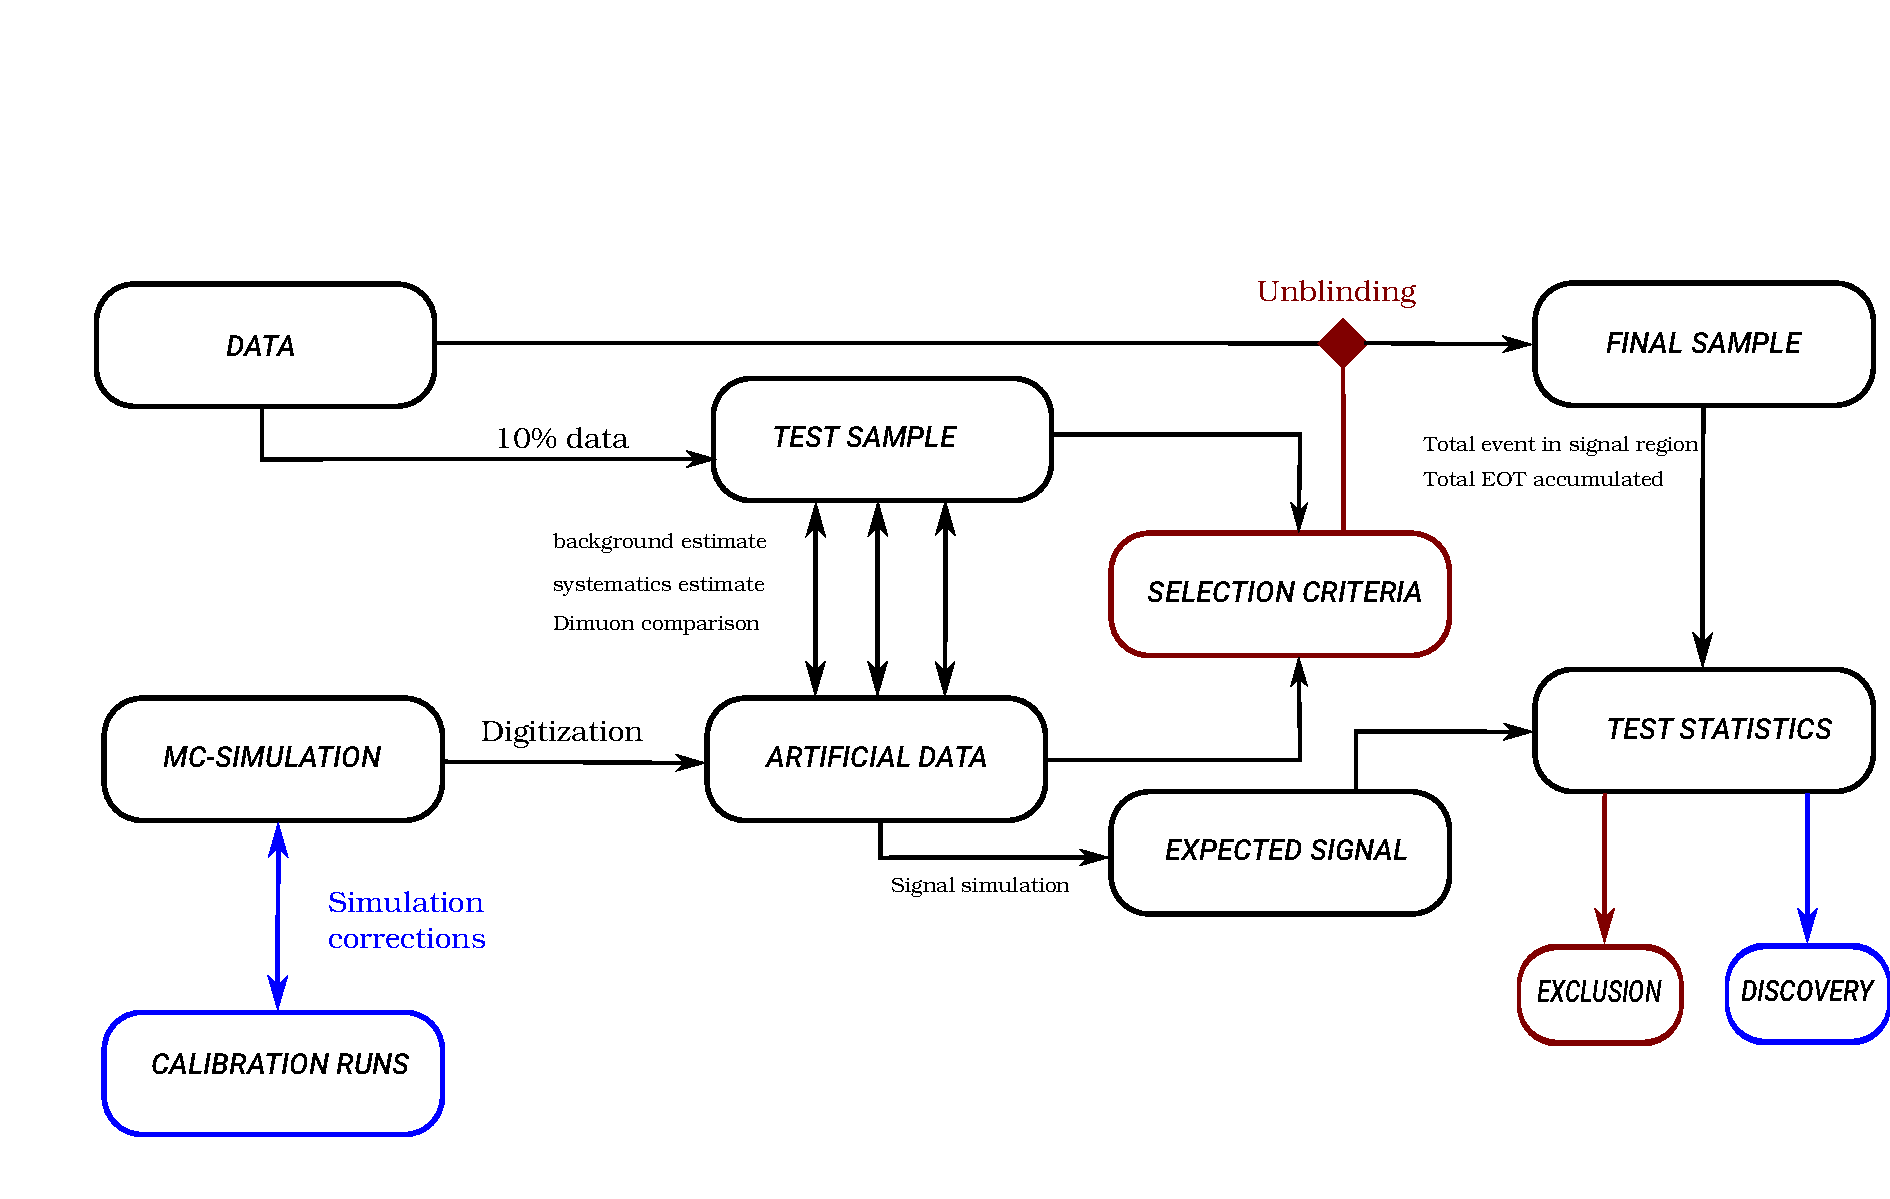
\includegraphics[scale=0.4]{\pdirthree/analysis-chart.pdf}
  \caption{Flowchart of the NA64 analysis.}
  \label{fig:analysis-chart}
\end{figure}

\section{Geant4 simulation of the experiment}
\label{ch3:sec:geant4}

The first ingredient for our analysis is Monte Carlo simulation to reproduce the particle interactions in our setup. This task can be divided into three subtasks:

\begin{enumerate}
\item A code to simulate particle interactions inside the NA64 setup.
\item A code to reproduce the detector response in our setup.  
\item A code that describes in detail the physics of $A'$.
\end{enumerate}

The first task is handled by the Geant4 library\cite{AGOSTINELLI2003250}. Geant4 software includes facilities to handle the geometry description, particle tracking, and run management. To produce a simulation, the end-user must provide an accurate description of the setup, a list of the interactions that need to be simulated, and the description of the primary particle, in terms of particle type\footnote{For a list of available particle and the explanation of the numbering scheme, see \cite{geant4-pdg}}, initial momentum and initial location.

The setup is described using different C++ classes to detail the precise geometry of each detector. To each geometry, a logical volume is assigned, which details the property of the geometrical object. In most cases, this means the atomic number Z, the mass number A, and the density of the material. These properties were taken from the NIST database \cite{nist-database} unless more reliable information (coming from example from the manufacturer of the detector) was available. In some cases, for example to simulate the vacuum and the gas detectors, pressure and temperature are also described using in-situ measurements. Finally, detectors are placed in the simulation using measurements done with a tape (with a precision $\sim$1 \si{\centi\meter}). For the trackers, an additional measurement was performed by the H4 meterology team with a precision of 0.5 \mmi \cite{meterology-measurements} later improved with an alignment procedure performed by the CORAL software \cite{ABBON2007455}. 

A physics list is then provided to simulate the relevant physics in the virtual setup. The physics list used in the simulation is the \textit{\textrm{FTFP\_BERT}} modular physics list, which is recommended for high-energy physics experiments \cite{ALLISON2016186}. This physics list combines an excellent description of electromagnetic physics and a description of the inelastic hadron-nucleus processes based on the Fritiof Parton Model (FTF) \cite{Uzhinsky:2013hea}, Bertini intranuclear cascade \cite{Heikkinen:2003sc} and Precompound models \cite{Apostolakis:2009zz}. Because of the complexity of these models and the absence of a precise theory of QCD at low energy, the description of the inelastic scattering for hadrons can still be problematic and a cause of systematic errors in the experiment. As we will see in Sec.\ref{ch3:sec:geant4-hcal-corr} this problem is addressed by correcting the model using data from the calibration run. 

What remains is to add the $\DM$ physics description to Geant4. This is currently done by an additional code that describes Dark Matter in a modular way following Object Oriented style of C++. This allows for the description of many Dark Matter candidates inside the same framework. The code has the following functions:

\begin{enumerate}
\item Compute the total cross-section of $\DM$ emission as a function of the properties of the target nucleus (namely Z, A, and density $\rho$) and the primary energy.
\item Decide if the emission of $\DM$ is happening inside a specific Geant4 step by throwing a random number.
\item Sample the energy and angle of the final state.
\item Compute the decay time in the laboratory system if the model predicts a visible decay and pass the information to Geant4.
\end{enumerate}

An instance of the Dark Matter class is called at the start of each run performed by Geant4, initialized with specific parameters of $\epsilon$ and $m_{\DM}$. The method of the class is then called at each step involving\footnote{In some cases this is called also for $\mu^-$/$\mu^+$ if the interaction is possible. In Sec.\ref{ch5:sec:muon-mode-setup} a setup to probe models with such interaction will be presented.} an $e^-$/$e^+$ to calculate the total cross-section and to decide if emission is performed. After that, energy and angle are sampled using a distribution $E_{\DM}(E_{e^-}, \theta_{\DM})$. In the case of the invisible mode, the energy of $\DM$ is subtracted to the particle who emitted it and its momentum recalculated. No new particle is created inside the simulation, as the NA64 experiment assumes the decay product $\dmchi$ to punch-through the setup with no further interaction. In the case of the visible mode, the decay length of $\DM$ is computed as a function of its energy and parameter, and an $\ee$ pair is created inside the decay volume by sampling the corresponding decay distribution in that region. A weight corresponding to the probability of $\DM$ to decay inside the fiducial volume (which is simply the normalized integral of the decay distribution along the decay volume) is saved as meta-information of the event and later used to correct the signal yield.
The differential cross-section and precise energy spectrum of $\DM$ were initially calculated using the IWW-approximation described in Sec.\ref{ch1:sec:dm-u1model}. In our new analyses, this estimate was improved using a complete tree-level calculation of the cross-section. This correction decreased the expected signal yield for mass larger than 10 MeV but increased it for mass smaller than 5 MeV \cite{DMsimulation}.

\begin{figure}[htb!]
  \centering
  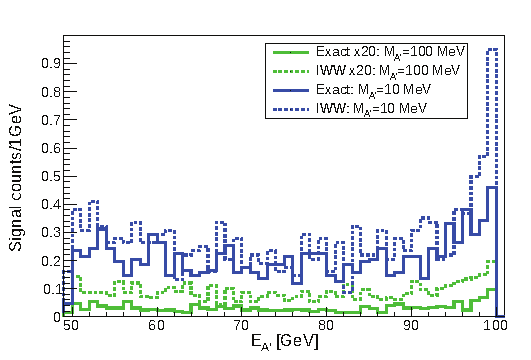
\includegraphics[width=\textwidth]{\pdirthree/DM-cs.pdf}
  \caption[IWW vs tree-level energy spectra]{Comparison of the energy spectrum of the emitted $\DM$ for a dark photon mass of 100 \mev and 10 \mev. The spectra are calculated using the IWW approximation (dotted line) and an exact tree-level calculation (continuous line) \cite{DMsimulation}.}
  \label{fig:dm-iww-tl}
\end{figure}


Finally, a biasing system was added to the code to increase the cross-section artificially. This is required to simulate efficiently the signal without the need of extremely large simulations. A correction factor $N_{norm}(\epsilon_{bias},m_{\DM})$ is calculated by the code and saved as metadata in the output. This factor is then used in the analysis of the simulations to correct for the artificial increase of the $e^- Z \to e^- Z \DM$ cross-section. The number of $\DM$ simulated scales linearly with $N_{norm}$, allowing a quick correction of the signal yield. The most relevant number for this is the expected number of $\DM$ produced normalized to the total EOTs, which we will call $\dmpereot$. This can be calculated simply from the output of the simulation using the following equation:

\begin{equation}
  \label{eq:1}
  \dmpereot = \frac{N_{norm}}{N^{tot}_{sim}} \times \sum^{n=N}_{i=0} \omega_i
\end{equation}

Where $N^{tot}_{sim}$ are the total number of events simulated, and $\omega_i$ is the weight associated with an event. For an event without $\DM$ production or that did not pass the selection criteria, this weight is zero. Else, the weight assumes a value between 0 and 1, which corresponds to the probability of $\DM$ to decay in the fiducial volume. In the case of an invisible decay, the number is always 1, since missing energy will always be present if the events pass all selection criteria. For the case of the visible mode, the number is set to the probability of $\DM$ to decay inside the fiducial volume mentioned back in chapter \ref{chapter1}. This corresponds to the integral of the decay spectrum between the last layer of the WCAL and the scintillator (S$_4$) placed at the end of the vacuum tube.

The final ingredient to start the simulation is an input particle to trigger the whole machinery. This is done using electron and hadron calibration run to extract a reliable beam profile. Hadron and electron beams are quite different from each other\footnote{This feature can also be used to cross-check the contamination of each of them, see Sec.\ref{ch3:sec:dimuons}}. For the case of hadrons, the beam is parametrized as an ellipse, with total width in the X-direction of 14.5 $\mmi$ and 6 $\mmi$ in the Y-direction\footnote{X being the coordinate aligned with the direction of the bending inside the magnetic field}. In the case of electrons, the parameterization use a 2D Gaussian distribution with $\sigma_x$=4.13 $\mmi$ and $\sigma_y$=1.4 $\mmi$. In both cases, the entrance angle of the particle is assumed to be uncorrelated with its initial position, and is parametrized with a Gaussian of width $\sigma_r$=0.4 \mrad. These parameters were obtained by fitting the beam profile recorded by the Micromegas in the calibration runs with a Gaussian in both projections. The fit was performed using the two Micromegas placed upstream the magnet and agreed within 5\% error.

\subsection{Reconstruction and digitization}
\label{ch3:sec:geant4-digitization}

The output of Geant4 can be divided into three different categories:

\begin{itemize}
\item Energy deposited in the active area of a scintillator counter or a calorimeter.
\item Hit information of a particle passing through the active area of a tracking chamber.
\item MC truth information regarding the event, including all the kinematics of the $\DM$ if it was emitted.
\end{itemize}

The first type is straight-forward. Each time a step is computed inside a sensitive detector, the energy deposited in the volume is added to some specific counters which are saved at the end of each event. At this point, some detector effects are already accounted for. Only the energy in the active part of each calorimeter is recorded, and the total sum of the energy deposited is corrected using a calibration constant which corrects the energy output to reflect the initial particle energy. Additionally, Birks law \cite{NYIBULE2014141} is implemented in the HCAL to correct for the propagation of optical photon in the WLS until the PMTs, using an attenuation length of 30 \si{\centi\meter}. This effects correct for the different light yields between $\pi^-$ and $\mu^-$, since in the case of $\mu^-$ the energy is deposited the full length of the detector evenly.

To reproduce tracking detectors, every time a particle crosses the gas volume of a gas chamber, multiple pieces of information are saved:

\begin{itemize}
\item x-y-z position of the particle at the beginning of the step.
\item The energy of the particle responsible for the hit.  
\item The energy deposited in the gas during the step.
\item The PDG number of the particle \cite{particle-numbering-scheme}.
\end{itemize}

These data define a structure called \textit{MChit}, which is used by the reconstruction algorithm to reproduce both hits and tracks in the same format of the data. This algorithm was developed during my thesis to improve the Digitization procedures. It works as follow:
\begin{enumerate}

\item Hits with an energy deposited in the volume smaller than the minimum amount to start the ionization inside the gas are removed. Practically, this threshold was set to 2 keV based on previous studies performed for MM \cite{IGUAZ20121079}. A similar value is assumed for the GEM detector as well.
\item Multiple \textit{MChit} are merged if they are found to be closer than a fixed distance. This distance is conservatively set to be 2 $\mmi$  for MM and 1.75 $\mmi$  for GEM. The new x-y position of the hit is computed using the weighted average of each hit position, where the weight is defined by the energy deposited inside the gas.
\item The x-y coordinates of the hits are transformed into the plane of the detectors using a simple matrix multiplication $u_{hit} = M_{uv}(\theta_{uv}) \cdot v_{hit}$ where $u_{hit}$ is the hit position in the detector coordinate system and $v_{hit}$ is the same vector expressed in the laboratory system. The Matrix $M_{uv}(\theta_{uv})$ is the rotation matrix of the $O(2)$ group where $\theta_{uv}$ is the angle between the axis of the detector and the axis of the laboratory system.
\item Each coordinate on the detector plane is treated separately. To reproduce the genetic multiplexing of the MM, each physical strip is mapped to its corresponding channels, and a 64-dimension vector is obtained as output. Noise is also added to each channel using the same pedestal measured in the sparse mode of the APV chips.
\item  The charge vector is used as input for the same clusterization procedure used for the data. In the MM detector, the clusterization is fully reproduced. the physical cluster is parametrized by a Gaussian, and the charge is distributed on the physical strips starting from the hit center. The total charge of the cluster is decided starting from the total energy deposited in the gas volume which is it into ADC counts. The constant of conversion is computed using the data of the electron calibration runs. The procedure for the GEM is more direct and only involves the smearing of the initial true hit position using a Gaussian distribution with a width corresponding to the hit resolution of the GEM detectors. This was estimated to be $\sigma_{GEM} \approx 80$ $\mum$ using the Three Layer Method \cite{Bortfeldt:2014vvt}.
\item After the clusterization is performed, two set $X_n$ and $Y_n$ of positions are extracted from the two planes and combined\footnote{In the most common case of just a single primary present upstream the ECAL, this association is trivial, since only one hit per plane is present.} in the set of hit candidates $(X;Y)_n$. A hit number per plane larger than five, other than being rare ($\lesssim$0.1\%), is not relevant for $\DM$ searches and hence rejected in the reconstruction. The hits candidates are then used as input of the tracking or vertexing procedure. The total momentum of a track is calculated from the displacement after passing through the magnetic field of the MBPL (see Appendix.\ref{AppendixD}). The vertex reconstruction is more involved but starts from the same input above. The procedure is described more in detail in Sec.\ref{ch3:sec:vis-mode-tracking}.
\end{enumerate}

Completed the procedure, these quantities are saved in a tree structure implemented in ROOT \cite{root} that is equivalent to the one used for the data. A shower profile analysis is also performed at this step (see Sec.\ref{ch3:sec:bkg-ecal-profile}) and added to the tree. This design allows using the same analysis to study MC and data without the need of changing the code.

The simulation code was also optimised to correct effects observed in data during calibration runs. In the next section, we will provide a specific example of this, where the hadronic model was modified to improve the agreement between simulation and data of the stopping-power observed for hadrons.

\subsection{Correction of longitudinal shower profile in the Hadronic calorimeter}
\label{ch3:sec:geant4-hcal-corr}

In this section we provide a specific example of how the simulation is corrected using data from the calibration runs that was part of my work. In this instance we improve the energy deposited inside a calorimeter in events with intranuclear inelastic scattering. A large amount of events where an incoming hadron deposit all its energy inside an electromagnetic calorimeter was observed in the simulation and not reproduced in the data.
% The reason of this deviation might be that most of hadronic models are optimized for a scenario where $\lambda_{int}$ of the target is large enough to stop completely the incoming hadron on average, which is not the case for the ECAL or the WCAL. As large em-shower triggered by hadrons is a source of background in the visible mode, this comparison is particularly significant to estimate the background of this mode precisely.

We compare the data and predictions by simulating a sample of $\pi^-$ and compare the distribution with the data of an hadron calibration run and do the same for $e^-$. The result of this first comparison is shown in Fig.\ref{fig:ecal-comp}. In the first plot, we see the energy deposited in the WCAL for electrons measured in the calibration run compared to what is predicted by our MC. As expected because of the QED nature of the process, the two distributions agree quite well in the core, with some minor disagreement in the tail mostly due to pileup. On the other hand, even after accounting for the detector corrections, we can see that there is a fundamental disagreement at the end of the spectrum when the comparison is performed with pions, specifically in the region relevant for deep inelastic scattering. Since the disagreement is large when all the nominal energy of the beam is deposited inside the target, the disagreement appears to be caused by some electron contamination in the hadron beam. However, the data were filtered by requiring less than 1 MeV energy deposited in each SRD counter facing the beam inlet. This reduces the contamination conservatively at a level $<$0.01\%, which is far below the disagreement observed. A faulty calibration is also unrealistic since the agreement with electrons is excellent in that energy range. The simulation systematically overestimates the number of events in the region where most of the energy released in the inelastic scattering is emitted in the form of $\pi^0$,$\eta$, $\eta'$ which trigger an em-shower completely contained in the calorimeter.

\begin{figure}[bth!]
  \centering
  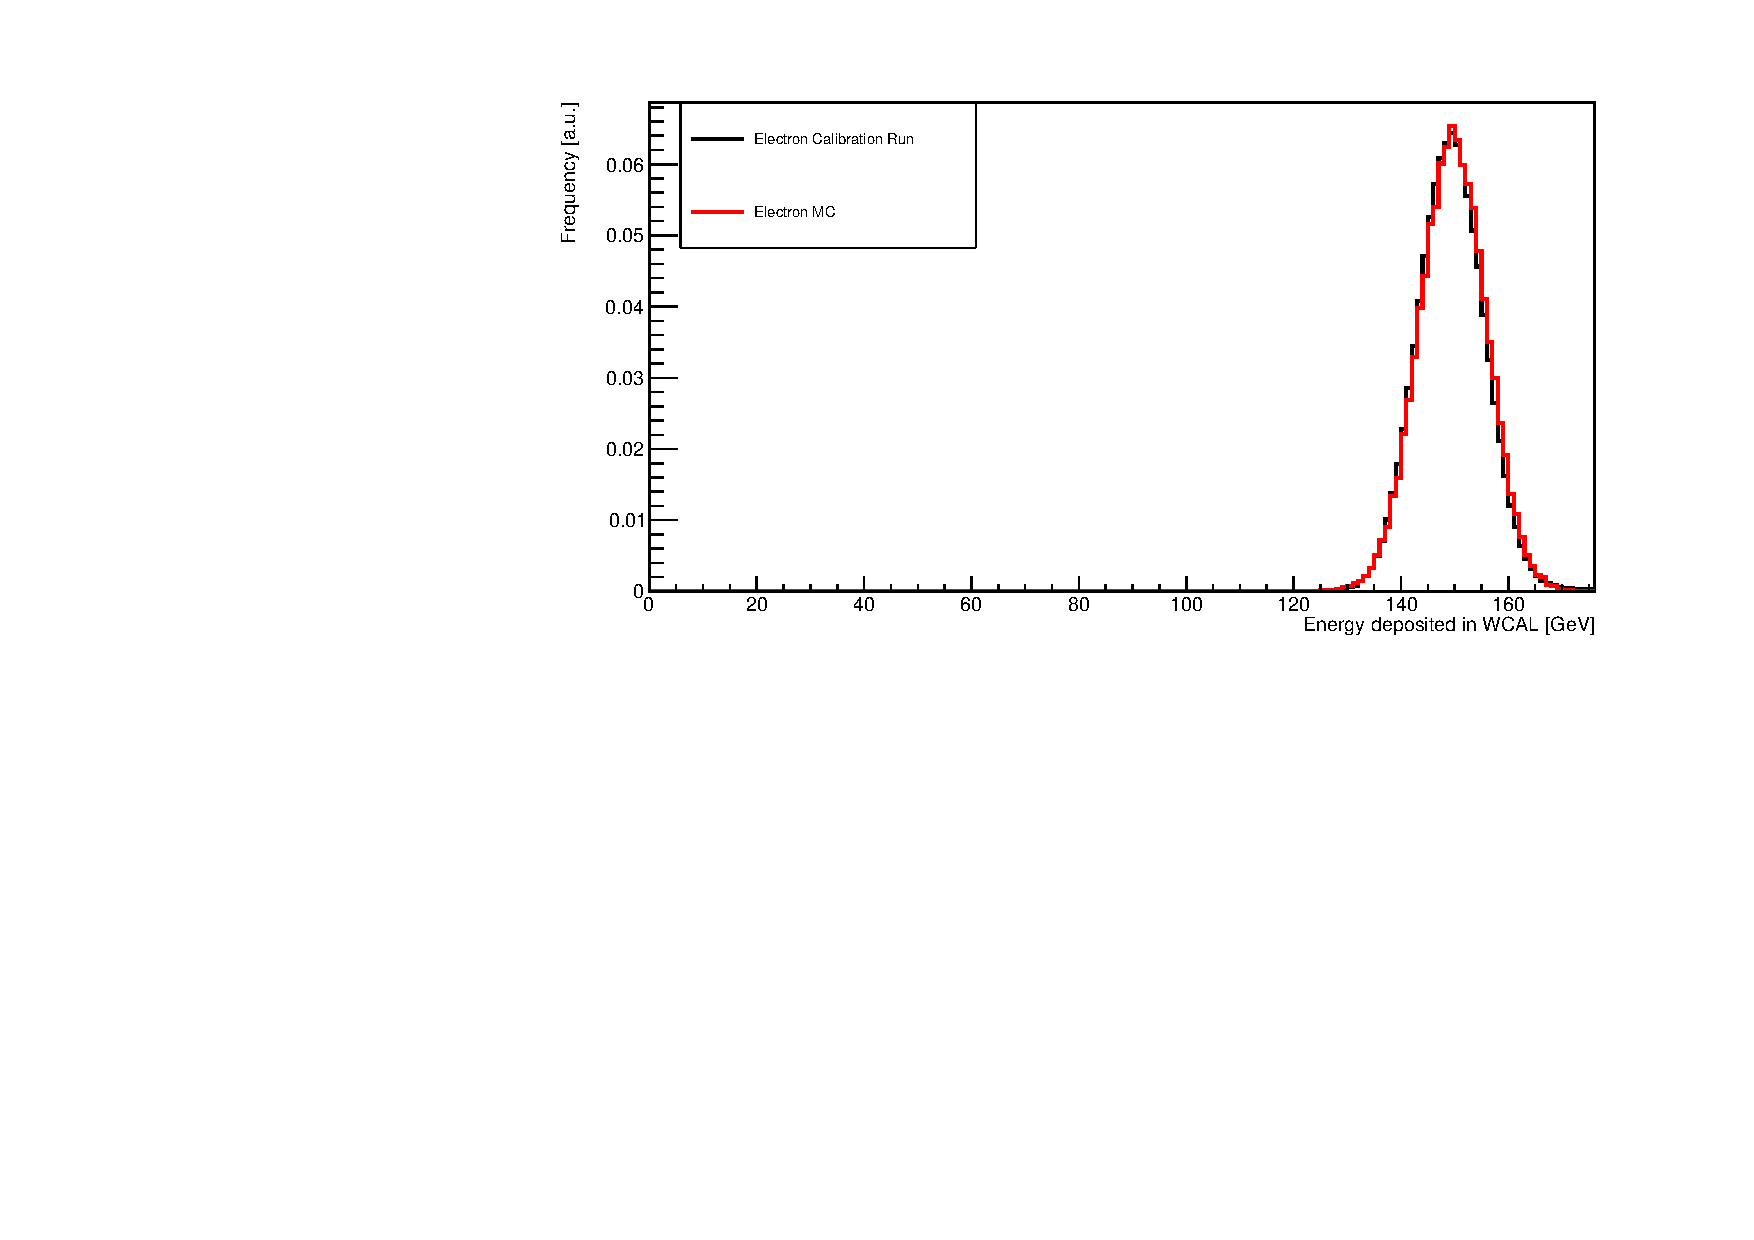
\includegraphics[scale=0.6]{\pdirthree/wcal_elec_comp.pdf}
  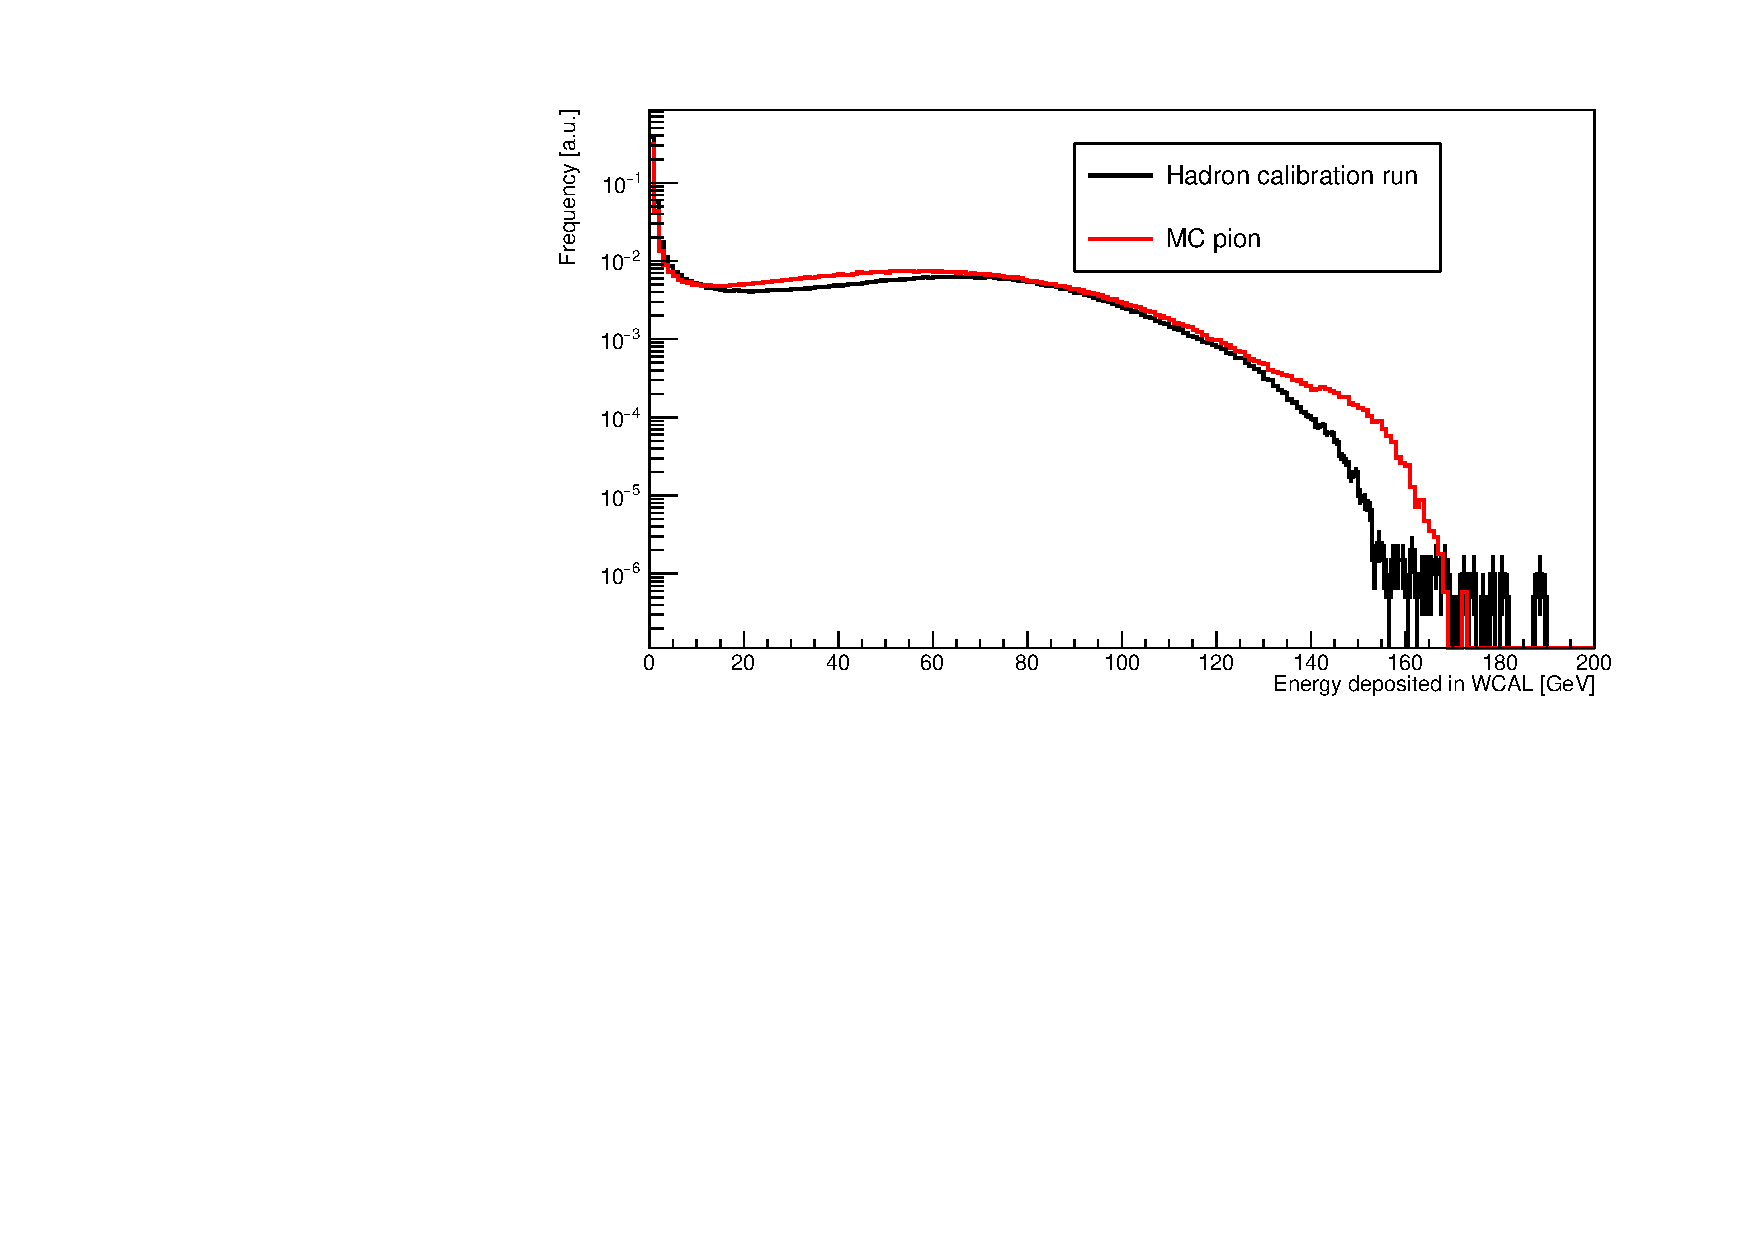
\includegraphics[scale=0.6]{\pdirthree/wcal_pion_comp.pdf}
  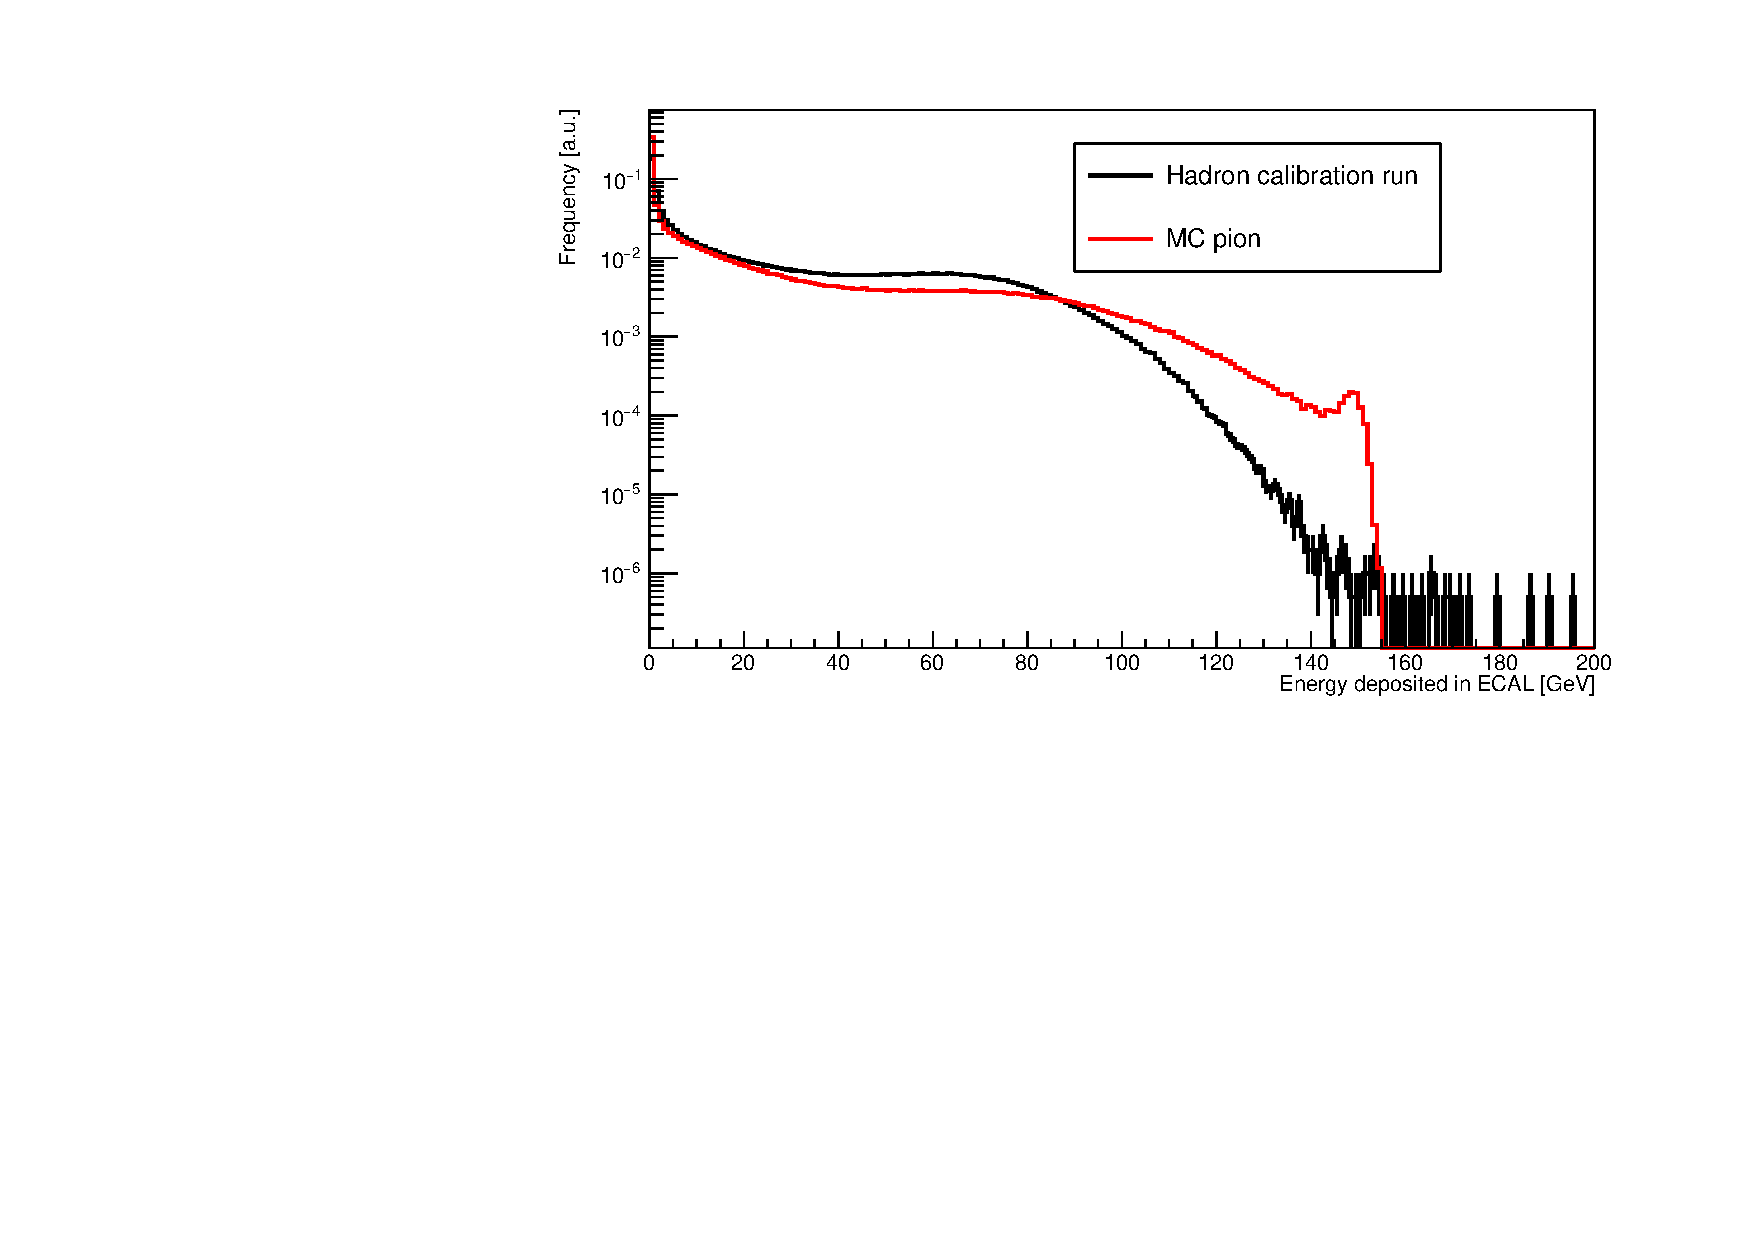
\includegraphics[scale=0.6]{\pdirthree/ecal_pion_comp.pdf}
  \caption[MC/DATA Comparison of $\pi^-$ in ECAL and WCAL]{Comparison between MC and data for different detectors and different runs. Top: WCAL energy deposited for electrons, Middle: WCAL energy deposited for hadrons, Bottom: ECAL energy deposited for hadrons.}
  \label{fig:ecal-comp}
\end{figure}

To investigate this mismatch, a complete comparison between different physics lists was performed to investigate 
different models. We used the energy deposited in the WCAL as a benchmark for this comparison, and simulate the interaction of $\pi^-$ using two alternative physics list. The \textit{QGSP\_FTFP\_BERT}, which uses the alternative Quark-Gluon String model to simulate hadrons at energy higher than 25 \gev, and the \textit{FTFP\_BERT\_TRV}, which uses the recommended Fritiof model but with an alternative method for the elastic scattering \cite{AGOSTINELLI2003250}. The result is shown in Fig.\ref{fig:geant4-hadron-plist}, the recommended physics list has the best agreement for high energy deposit, but for all three the disagreement remains significant. The QGSP model, although offers the worst prediction at high energy, has better agreement after in the range 25-80 $\gev$.

\begin{figure}[tbh!]
  \centering
  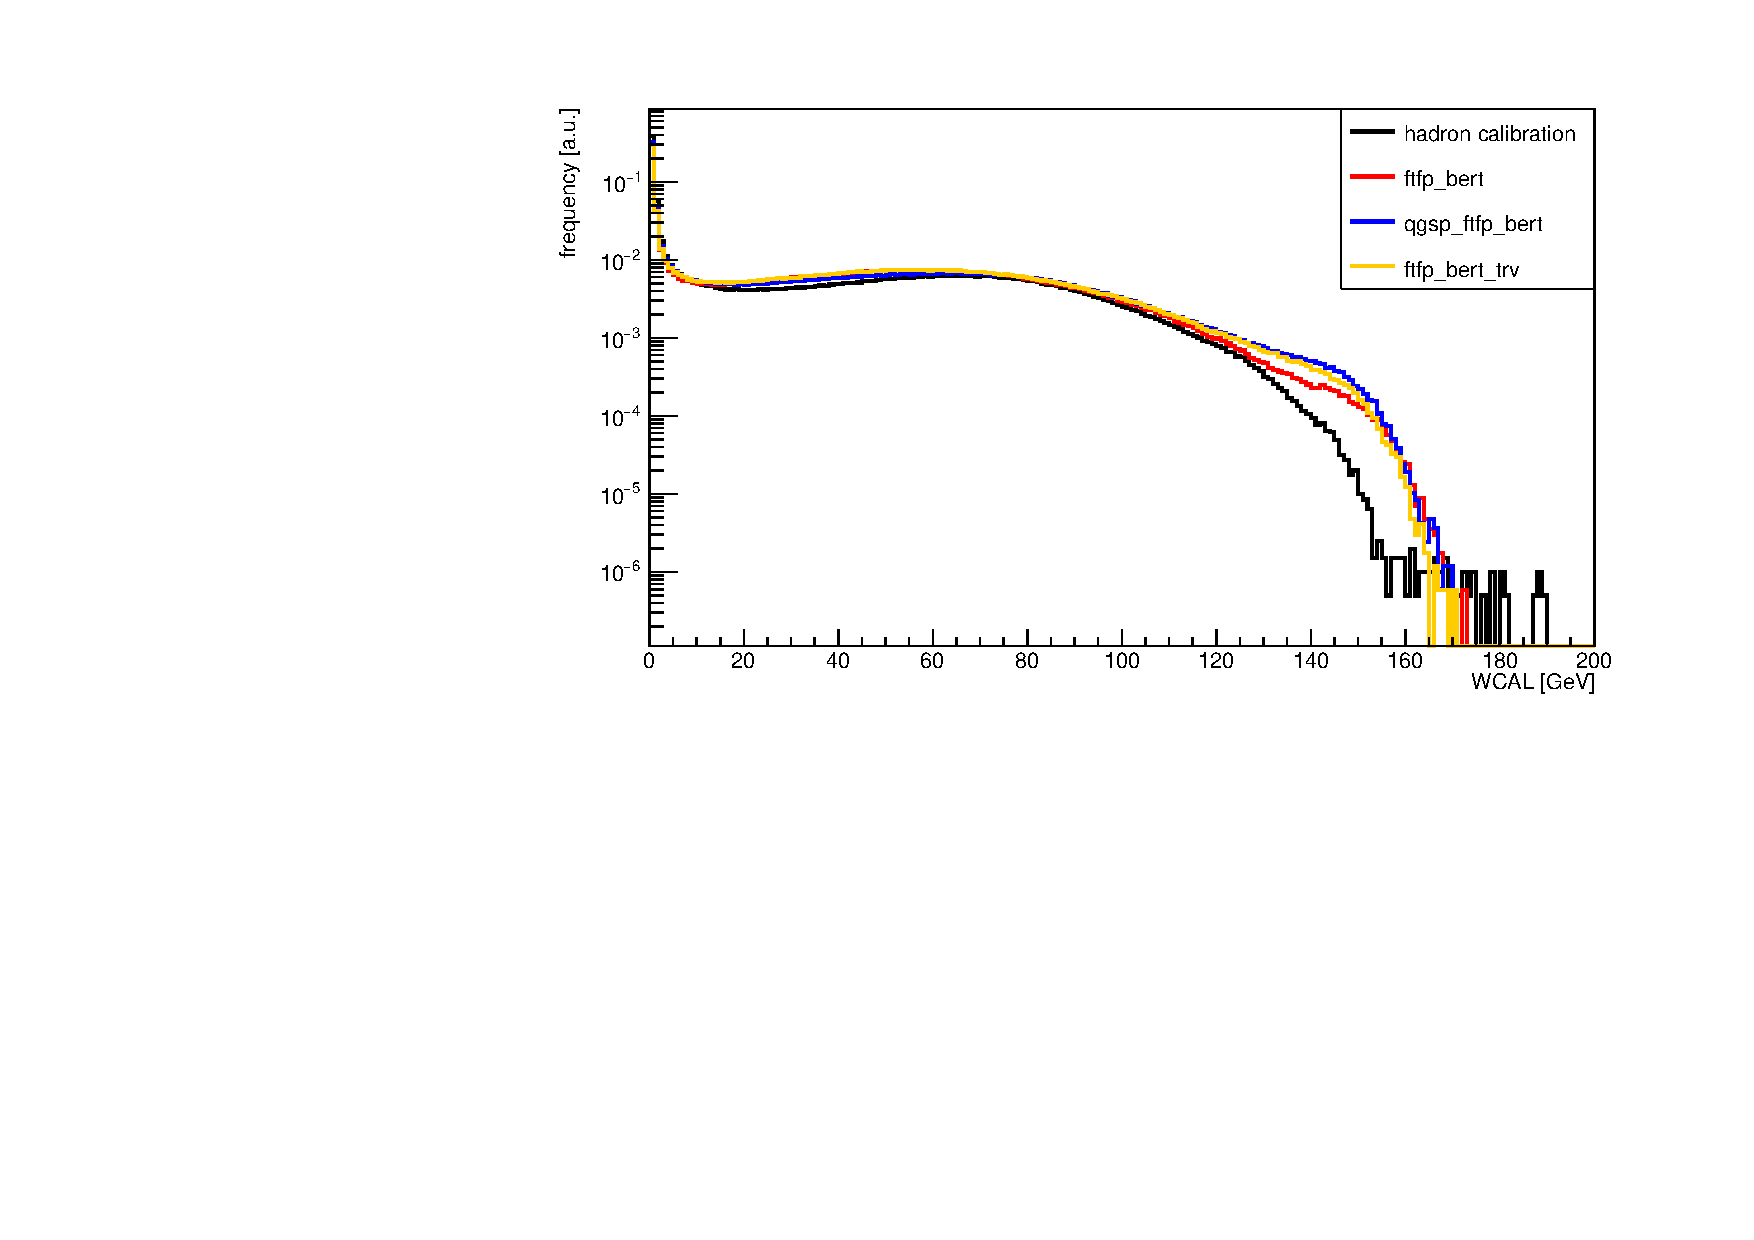
\includegraphics[width=\textwidth]{\pdirthree/physlist_v1.pdf}
  \caption[Comparison of physics list for $\pi^-$ in WCAL energy spectrum]{Energy deposited in WCAL for different physics lists. Data collected in the hadron calibration run in 2018 are plotted in black.}
  \label{fig:geant4-hadron-plist}
\end{figure}

The next test performed was to simulate different particles in the setup. The three main contributions to the beam impurities in H4 were simulated using the \textit{FTFP\_BERT} physics list: $\pi^-$, K$^-$, and p$^-$. Here a significant improvement is visible in the case of anti-proton (Fig.\ref{fig:geant4-hadron-particles}), where data and MC are compatible at the tail of the distribution. This would suggest that such an event is caused by charge-exchange interaction between pions and the target nucleus, enhanced for light mesons. To date, no proper treatment is offered by Geant4 for this process, which means the disagreement must be caused by an improper treatment of hadronization in the limit of diffraction,  where most of the energy is exchanged between two partons: one of the nucleus and one of the projectile impacting it. The discussion becomes here more complicated and requires the tuning of specific parameters inside the FTF model.  The \textit{FTFP\_BERT} physics list was modified as illustrated in Appendix \ref{appC:sec:ftfp-modifications} to experiment with different possibilities. The target diffraction and the projectile diffraction were switched on and off respectively to investigate the effect on the distribution.


\begin{figure}[tbh!]
  \centering
  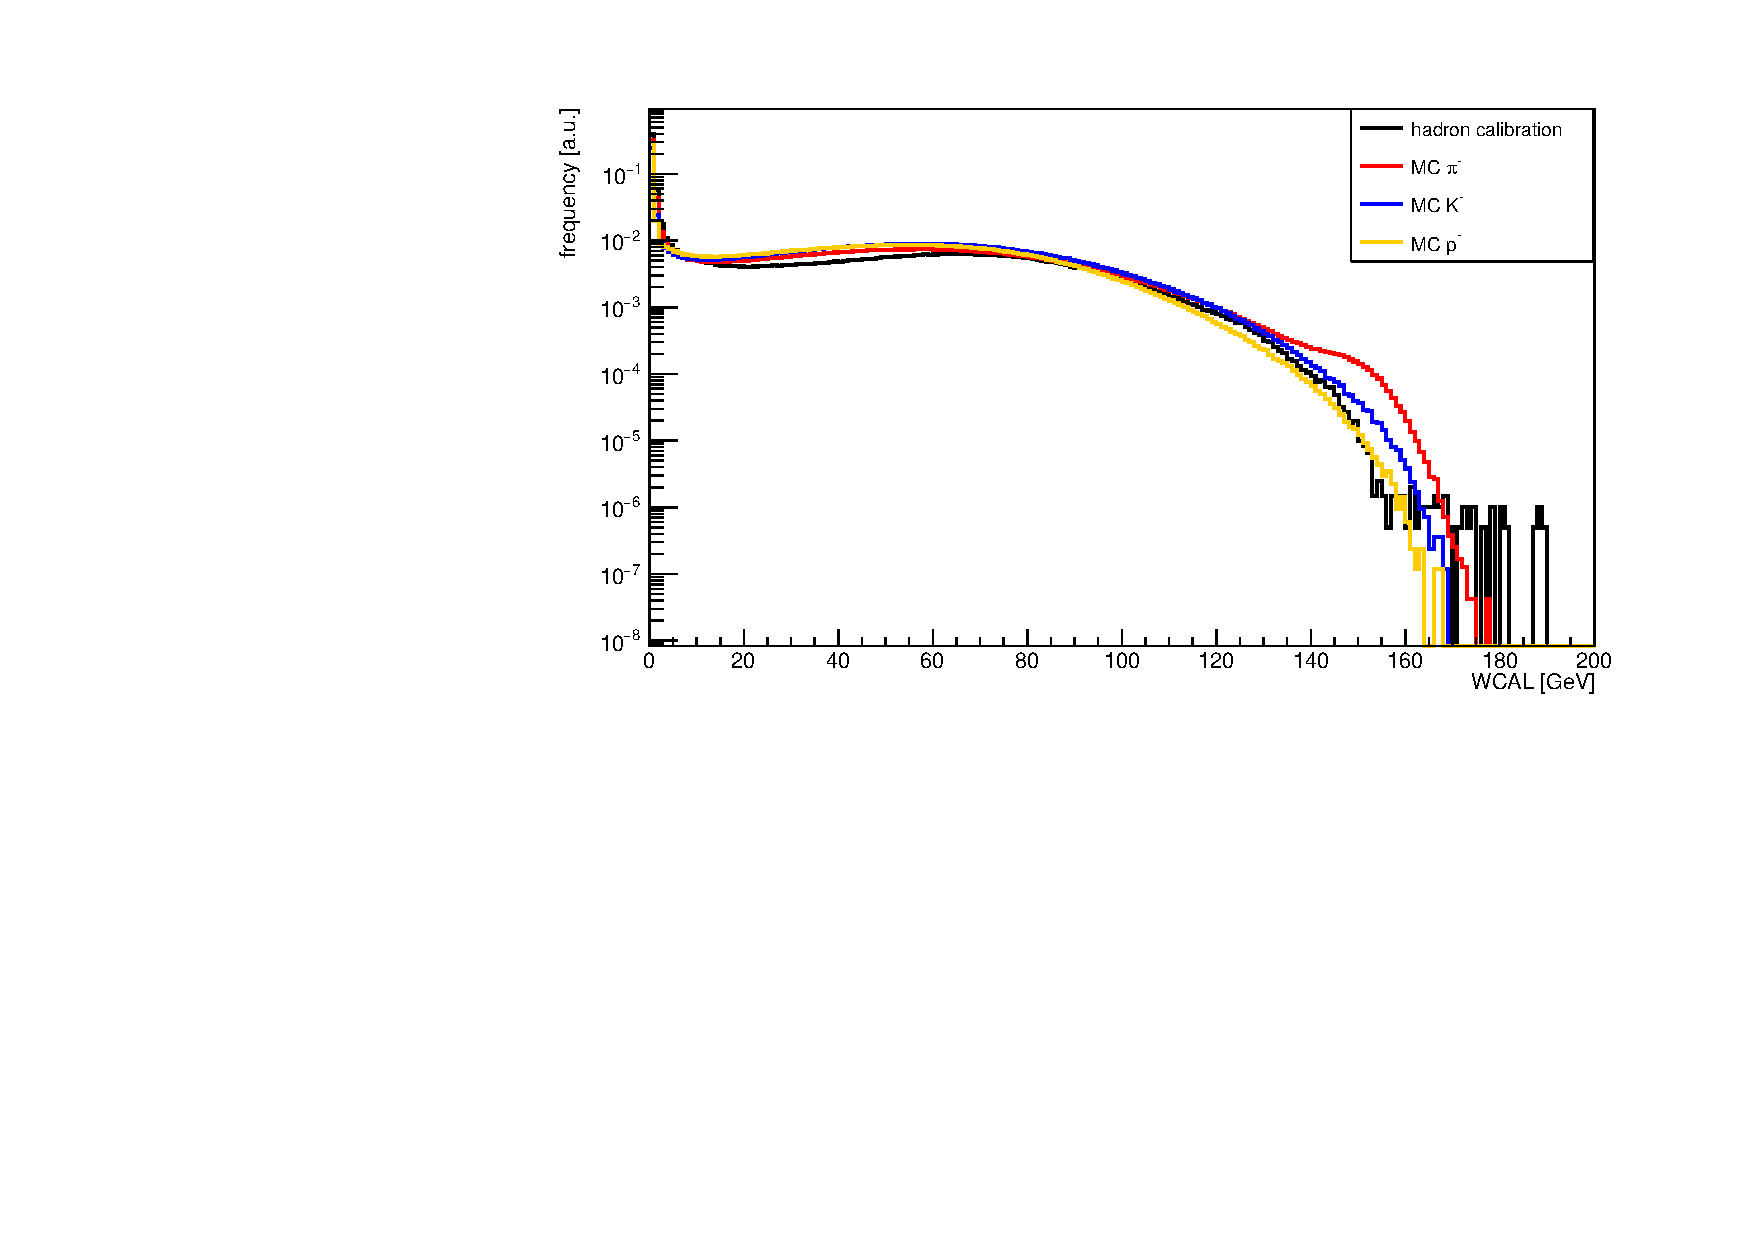
\includegraphics[width=\textwidth]{\pdirthree/physlist_particles.pdf}
  \caption[Comparison of different simulated hadrons in WCAL energy spectrum]{Comparison of different simulated hadrons in WCAL energy deposit.}
  \label{fig:geant4-hadron-particles}
\end{figure}

\begin{figure}[tbh!]
  \centering
  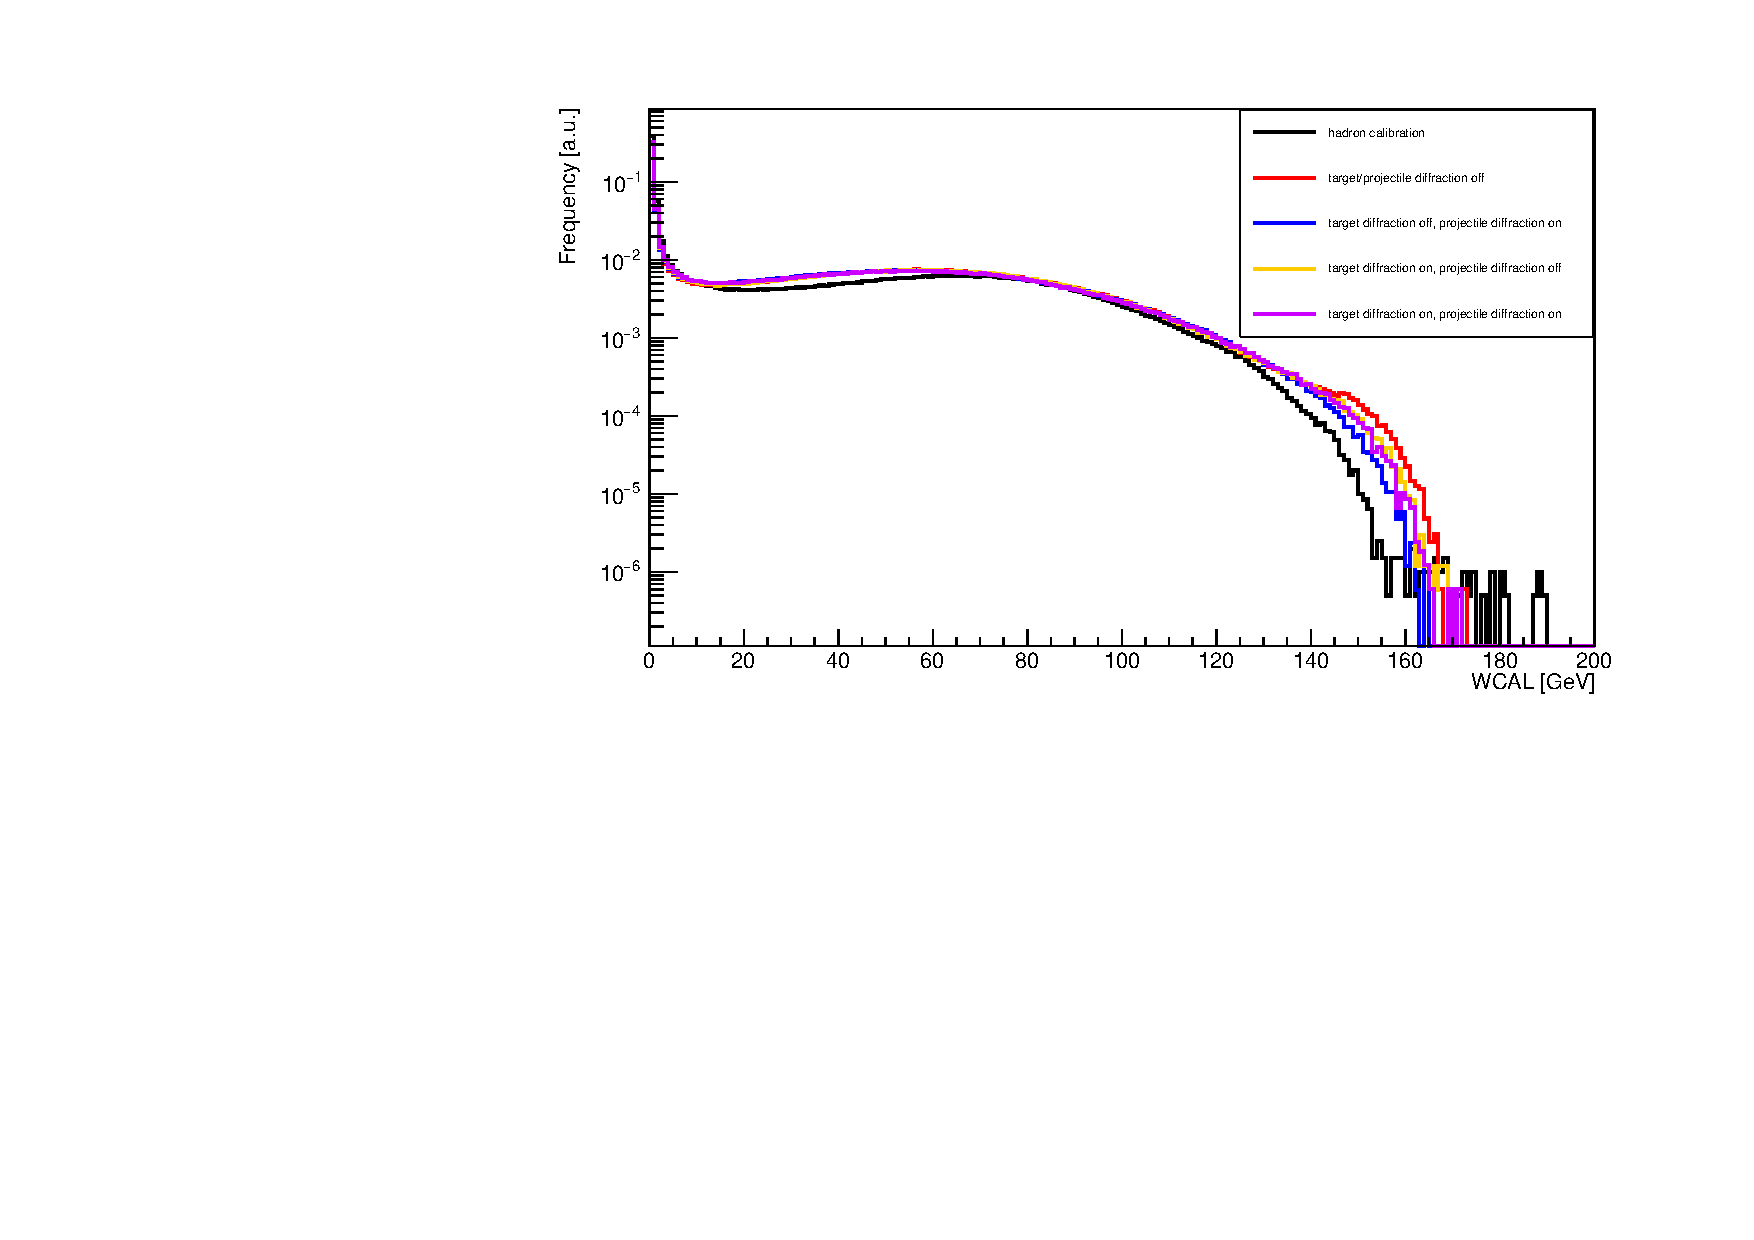
\includegraphics[width=\textwidth]{\pdirthree/physlist_diffraction.pdf}
  \caption[Comparison of different diffraction limits for hadrons in WCAL energy spectrum]{Comparison of simulated $\pi^-$ in WCAL energy deposit using the physics list $FTFP\_BERT$ using different parameters for the model. Main difference between models is the diffraction of target or projectile, which is switched on and off.}
  \label{fig:geant4-hadron-diff}
\end{figure}

The conclusion of this comparison (Fig.\ref{fig:geant4-hadron-diff}) is that the largest contribution to the disagreement comes from the projectile diffraction incorrectly excluded in the standard \textit{FTFP\_BERT} physics list, whereas target diffraction contributes instead negatively to the residual.

Some modifications of the \textit{FTFP\_BERT} were decided to improve the agreement in the distributions considered. The target diffraction was switched off, the projectile diffraction was switched on, and the parameters of the FTF model were modified to shift the behavior of $\pi^-$ to the one predicted for an anti-baryon. This is performed by acting mostly on the probability of each quark to be involved in the scattering and the average energy exchanged between partons. The final result is shown in Fig.\ref{fig:geant4-hadron-final}, the disagreement for the high-energy spectrum improves, with some overestimation of the probability of large inelastic scattering still present in the energy range 25-80 \gev. The disagreement for deposit larger than 20 $\gev$ is now $\sim$15\%, improved by a factor 2 compared to the original model.

\begin{figure}[tbh!]
  \centering
  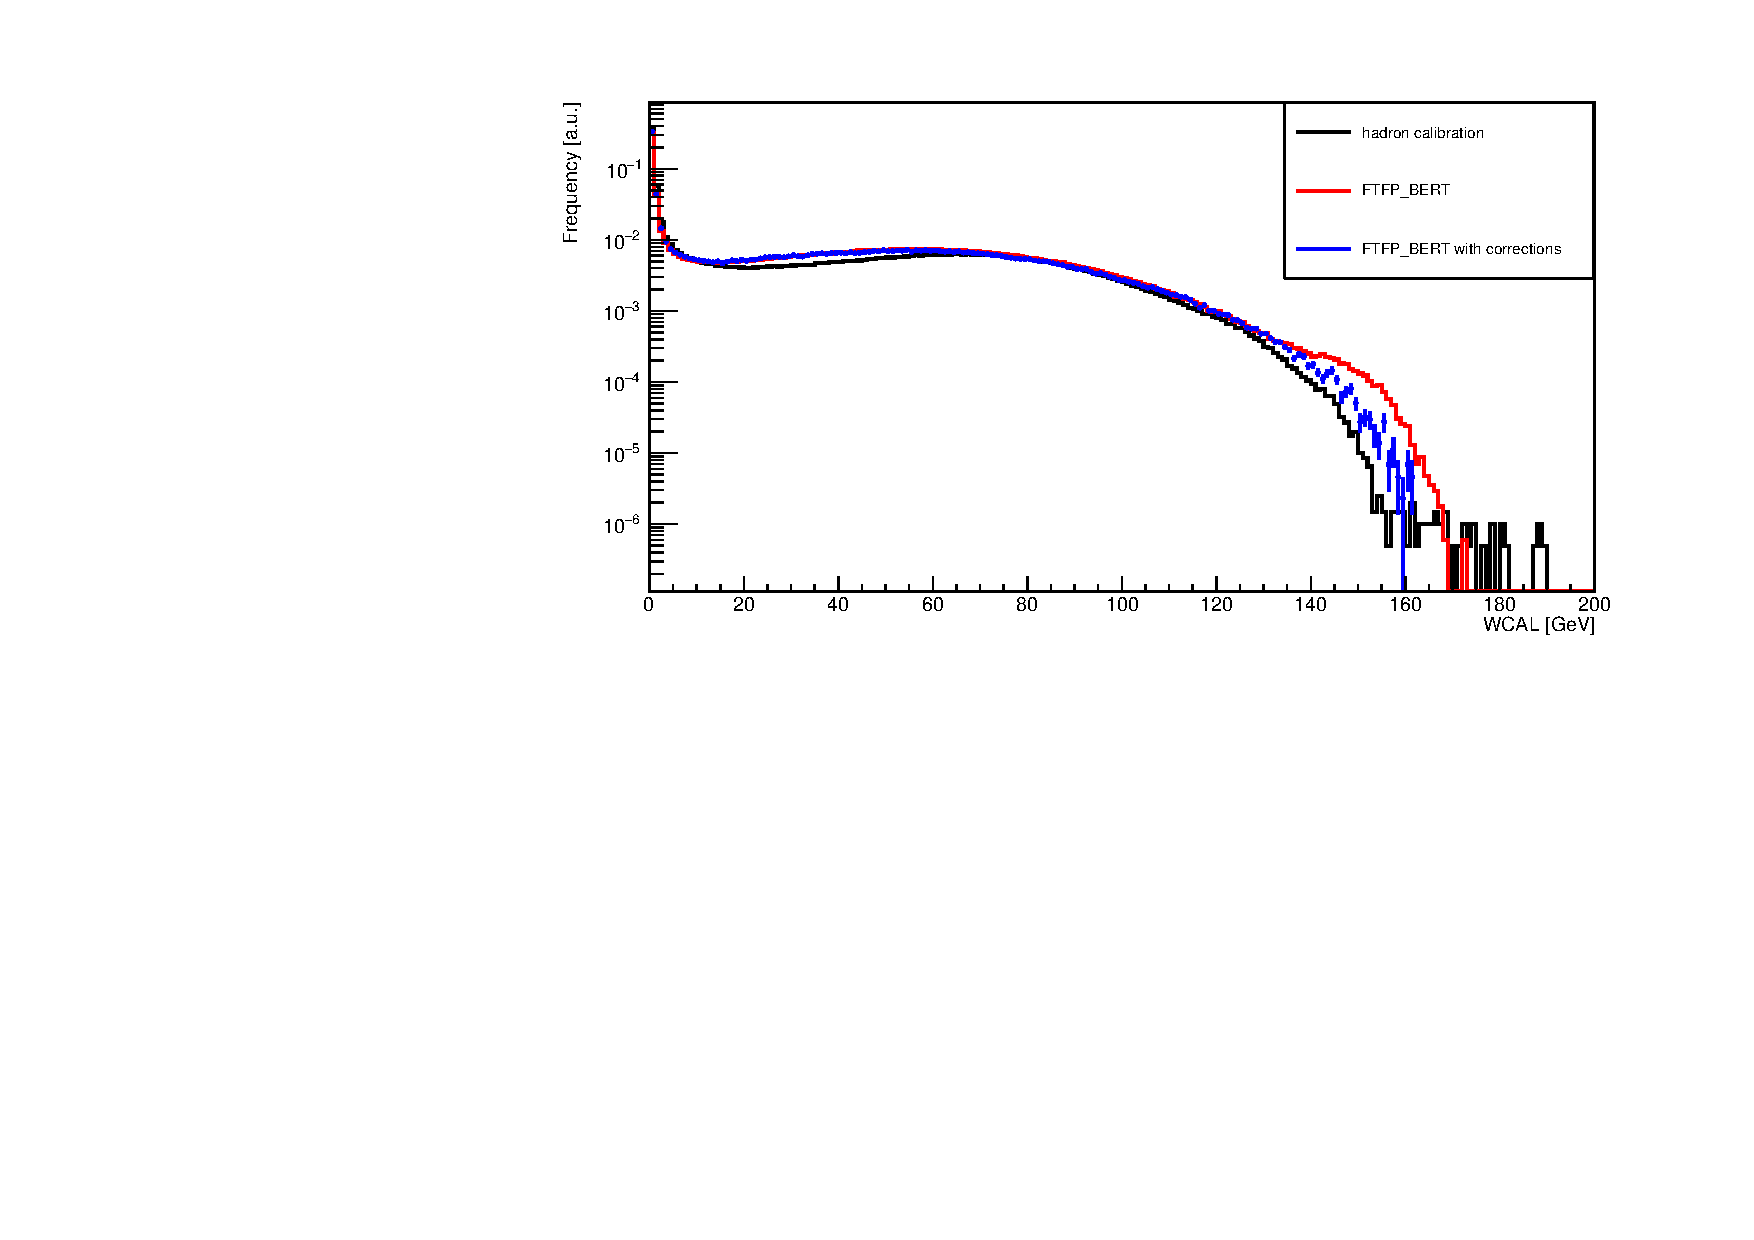
\includegraphics[width=\textwidth]{\pdirthree/final_comp.pdf}
  \caption[Comparison of hadron energy deposit after corrections]{Comparison between data (black line) and simulated $\pi^-$ in WCAL energy deposit using the physics list $FTFP\_BERT$ before and after corrections applied to the model.}
  \label{fig:geant4-hadron-final}
\end{figure}
\clearpage
\newpage
\section{Monte Carlo validation using $\gamma + Z \rightarrow \mu^+ \mu^-$ events}
\label{ch3:sec:dimuons}

The $\emu$ interaction consists of the rare production of a $\mu^+mu^-$ inside an em-shower after an incoming photon interacts with a target nucleus. The process of pair production is equivalent for all charged leptons (e,$\mu$,$\tau$) and has a cross-section in the order of $\sigma_{pair} \sim 4Z^2\alpha r^2_c$. Compared to the more frequent $\ee$ production, this interaction is suppressed by a factor ($m_e$/$m_{\mu}$)$^2$ = 2.34 $\times 10^{-5}$ because of the larger muon mass. This process is used both to validate the MC simulation and estimate the systematics of the experiment, as it shares many similarities to the signal under study:

\begin{enumerate}
\item Rare process produced inside an em-shower.
\item In first approximation, it can be computed inside the QED framework, hence with high precision.
\item The process penetrates very efficiently both the target and the HCAL modules. Each $\mu^{\pm}$ loses an energy $<250$\si{\mega\electronvolt} after its passage through the target, and $\sim$1.3 $\gev$ for each HCAL module encountered. 
\item While the energy spectrum of the emitted $\mu^+\mu^-$ is not equivalent to the one of $\DM$ \cite{dimuon-mc}, it spans the same energy region relevant for the $\DM$ signal.
%Hence, a comparison between MC and data for dimuons is an excellent test for the reliability of the MC.
\end{enumerate}

Additionally, because of the double MIP signature that the $\emu$ interaction leaves inside the VETO and the HCALs, this interaction can be easily distinguished from a signal event. The possibility of the leakage in the signal region was computed for both invisible and visible mode and was found not to be a relevant background (see for example Sec.\ref{ch3:sec:bkg:vis:elec}).

In Geant4, the process is described starting from the formula \cite{dimuon-mc}:

\begin{equation}
  \label{eq:sigma-dimuon}
  \sigma_{tot}^{\gamma \to \mu^+ \mu^-}(E_{\gamma}) = 4\alpha Z^2 r^2_c\int^{x_{max}}_{x_{min}} \left(1 - \frac{4}{3}x_+x_- \right) \log{W}dx_+
\end{equation}

Where $x_+$ the fraction of energy of the original $\gamma$ being transferred to the $\mu^+$ and $W$ is a function of $x_+$,$E_{\gamma}$, and the Z, A of the element, which also takes into account both the atomic-screening using the Thomas-Fermi model and the finite size of the nucleus. Some numerical values for this are provided in \cite{dimuon-mc}. To increase computation speed, a parameterization of Eq.$\ref{eq:sigma-dimuon}$ is used instead, with a precision greater than 2\%. After the dimuon pair is generated, the amount of energy transferred to the $\mu^+$ is decided by sampling the differential cross section\footnote{In this case, just the argument of the integral in Eq.\ref{eq:sigma-dimuon}} and the new particles are produced in Geant4. Since the interaction is approximately elastic, the relation $E_{\gamma} = E_{\mu^+} + E_{\mu^-}$ is used for the computation.

For a comparison between data and MC, $\emu$ interaction are collected from the complete sample of data collected for both visible and invisible mode using the criteria $1.2 \gev < E_{HCAL}^{1,2,3} < 6.35 \gev$ compatible with the passage of two MIPs in all HCAL modules. All selection criteria are then applied to the sample obtained, excluding energy deposited on the VETO (and W2 in the case of the visible mode). After that, the energy spectra recorded in the target is compared between data and MC. First, both samples are normalized to the same value to compare the shapes of the two spectra and check the reliability of the MC. After that, the two distributions are normalized to the number of EOT collected, the difference between the two is taken as a correction factor to the total number of EOT accumulated, as it shows some disagreement between data and MC prediction due to the systematics of the experiment \cite{na64-prd}. Correction factors can be derived from the detailed comparison of the energy deposited in the ECAL between data and MC. Each bin of the spectrum is compared and the ratio is computed using the formula:

\begin{equation}  
  \label{eq:RR-factor}
  \begin{aligned}
  &R_{data/MC} = \frac{n_i^{ECAL}}{n_{tot}^{ECAL}} \\
  &RR_i = R_{data}/R_{MC}
  \end{aligned}
\end{equation}

Inside the MC simulation, each event is weighted by the corresponding factor $RR_i$ as a function of the energy deposited in the target. Such corrections are different between runs and are mostly affected by the intensity of the beam and the variation of the trigger-threshold in the PS detector during data taking. These corrections typically reduce the signal yield by 5\%-10\%. Differences in reweighting between runs collected at the same intensity are taken as systematic errors, which amount to a maximum of 7\%\footnote{The precise error has a small dependence from the $\DM$ mass, for masses of $\simeq$10 MeV this error amount to 5\% \cite{na64-prd}.} An example of such comparison is shown in Fig.\ref{fig:dimuon-comp-invis}.

\begin{figure}[tbh!]
  \centering
  %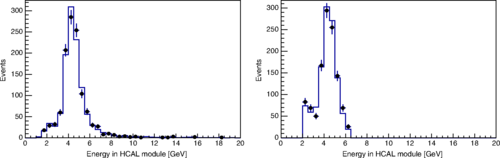
\includegraphics[width=\textwidth]{\pdirthree/dimuon-hcal-comp.png}
  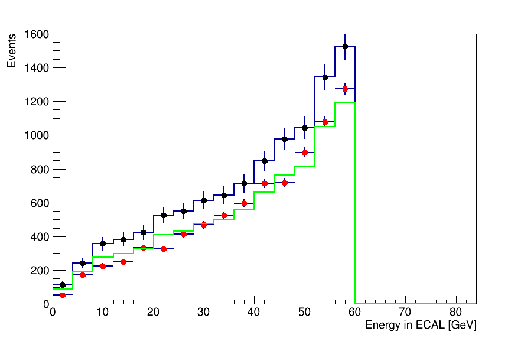
\includegraphics[width=0.45\textwidth,height=0.43\textwidth]{\pdirthree/dimuon-ecal-comp.pdf}
  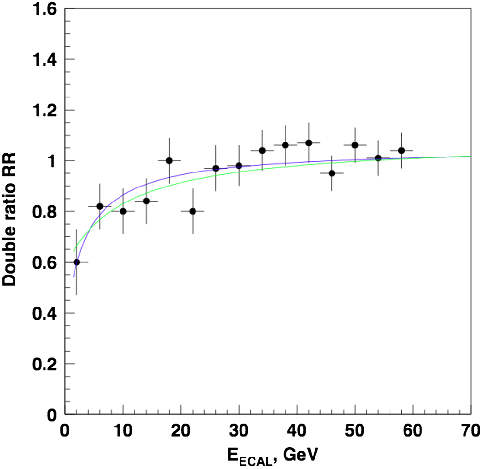
\includegraphics[width=0.45\textwidth,height=0.4\textwidth]{\pdirthree/dimuon-RR-comp.pdf}
  \caption[Dimuon spectra in ECAL for data and MC.]{Left: Distribution of energy deposited in the ECAL target by the scattered electron from the reaction $\emu$ selected from data (red dot) and MC generated event (green line). Data and MC are normalized to the same number of event. The unnormalized MC distribution is also shown with the corresponding error on the top histogram. Right: Ratio RR between MC and data efficiency of dimuon production as function of the energy deposited in the ECAL. The two color curves shows examples of empirical distribution of the values \cite{na64-prd}.}
  \label{fig:dimuon-comp-invis}
\end{figure}

\section{Background rejection methods}

Part of my work was also to improve the background condition. In this section, I will describe two methods developed during my thesis for this purpose.

The first method exploits the emission of synchrotron radiation by the electrons during their passage in the magnetic field to distinguish the ID of the incoming particle. The nature of this radiation is described more in detail in Appendix.\ref{appB:sec:sr}, together with the most relevant equation in the NA64 scenario. The method was tested using BGO crystals during the test beam performed in 2016 and resulted in a total suppression of hadrons of $p \simeq 10^{-5}$ published in \cite{Depero:2017mrr}.

The second method consists of a shower profile analysis to check the compatibility of the energy deposited in each cell with the one predicted for an em-shower. A set of measurement performed using calibration runs were used to build a model to predict the energy deposit as a function of the impact point of the incoming particle extrapolated from the Micromegas.  This method was documented in an official NA64 note \cite{na64-shower-profile}, and achieved a background suppression of $p \simeq 10^{-3}$.

\subsection{Heavy charged particle rejection using synchrotron radiation}
\label{ch3:sec:bkg-srd}

The rejection of the heavy charged particle is one of the main tools to reject the contamination of $\pi^-$,$K^-$, and $\mu^-$ present in the beam. The working principle of this method is simple in its approach. A particle traveling through a magnetic field will emit synchrotron radiation. With minimal assumptions, the total power after a full cycle can be calculated is the useful formula :

\begin{equation}
  \label{eq:srd-power}
  P = \frac{q^2 c}{6 \pi R^2}\frac{E^4}{m^4}
\end{equation}

Here R is the bending radius experienced from the particle when inside a magnetic field B perpendicular to its velocity. From this equation, we see that the total power scales to $P\sim E^4/m^4$. This both means that the technique is suitable for high-energy particle, as the signal will be boosted, and is useful to separate particles with large differences in the mass spectrum. The difference in mass between the electron and all other particles is so large in fact that effectively no radiation is emitted at the energy of the H4 beamline. 

Simulation of the expected SR signal was performed with the Geant 4 package\cite{ALLISON2016186,1610988,AGOSTINELLI2003250}.
The geometry of the NA64 experiment was coded in Geant 4, including the 200 $\mu$m mylar vacuum windows, the detailed composition of the trackers, scintillators and the residual gas was set at a level of $10^{-3}$ mBar as in the measurements. Saturation of BGO was taken into account using Birks' law with the constants taken from \cite{AVDEICHIKOV2002251}.

The expected SR spectra for pions and electrons with energies of 50 GeV and 100 GeV are shown in Fig. \ref{fig:SRspectrum}. The plot shows the expected dependence on the incoming electron energy in the emission spectra for the realistic experimental conditions. Moreover, the comparison between the SR spectra of pions and electrons illustrates clearly the principle of this technique that allows to discriminate between them by requiring an energy threshold in the synchrotron detector.  For pions, one can see that the probability of detecting an event with energy above 1 MeV is about $\sim 10^{-3}-10^{-4}$.
These SR-like signals originate from the interactions of the incoming pions with materials placed along the beamline. Although in first approximation the energy transfer due to ionization is in the order of few \si{\kilo\electronvolt}, rare high energy transfer is also possible. The distribution of such secondary electrons with
kinetic energy $T\gg I$, where $I$ is the mean excitation energy of the
atom/molecule, for a particle with velocity $\beta=v/c$ and charge $z$
passing through a material with atomic number $Z$, mass number $A$ and
thickness $dx$ is described by \cite{review-particle-physics}:
\begin{equation}
\frac{d^2N}{dTdx} = \frac{1}{2}K z^2 \frac{Z}{A}
\frac{1}{\beta^2}\frac{F(T)}{T^2}
\label{eqn:knock-on}
\end{equation}
The constant $K$ is defined as $K=4\pi N_A r_e^2 m_e c^2$ where N$_A$ is
the Avogadro's number, $r_e$ is the classical electron radius and $m_e$
the electron mass.
$F(T)$ is a spin-dependent factor, which in our case for $T \ll W_{max}$
is very close to unity. W$_{max}$ is the maximal energy transfer in a single collision to the
electron:
\begin{equation}
W_{max} = \frac{2m_e c^2 \beta^2 \gamma^2}{1+ 2\gamma m_e/M+(m_e/M)^2}
\end{equation}
For a $\pi^-$ at 100 GeV, $W_{max}$ is roughly 1 GeV which
covers completely the energy range where synchrotron radiation is
emitted. Eq.\ref{eqn:knock-on} is valid in the range $I\ll T \leq W_{max}$.
 \par 
Furthermore, Geant 4 reproduces the critical energy $E_c$ which divides the spectrum into two parts of equal power is:
\begin{equation}
E_c = \frac{3 \hbar c \gamma^3}{2R}
\end{equation}
with the reduced Plank constant $\hbar$ and the bending radius $R$. 
 For 100 GeV electrons in the  $B=1.7$ T bending field this corresponds to $E_c\sim$11.35 MeV. The expected mean energy of a synchrotron photon $E_m=E_c/\pi\simeq 3.6$ MeV is in very good agreement with simulation. The number of photons emitted per revolution in this energy range in the field of 7 \si{\tesla\meter} is defined as:
\begin{equation}
N_\gamma = \frac{5 \pi \alpha}{\sqrt{3}}\gamma
\end{equation}
where $\alpha$ is the fine structure constant. 
By scaling this equation for the fraction of the circle where the particles are inside the magnetic field, one obtains a mean number of emitted photon of about 24.
The SRD geometrical acceptance is about one third,  thus one can estimate that the sum of deposited energy is approximately 29.35 MeV in good agreement with the results of the simulation as shown in Fig. \ref{fig:SRspectrum}. 
 
\begin{figure}[htb!]
\centering
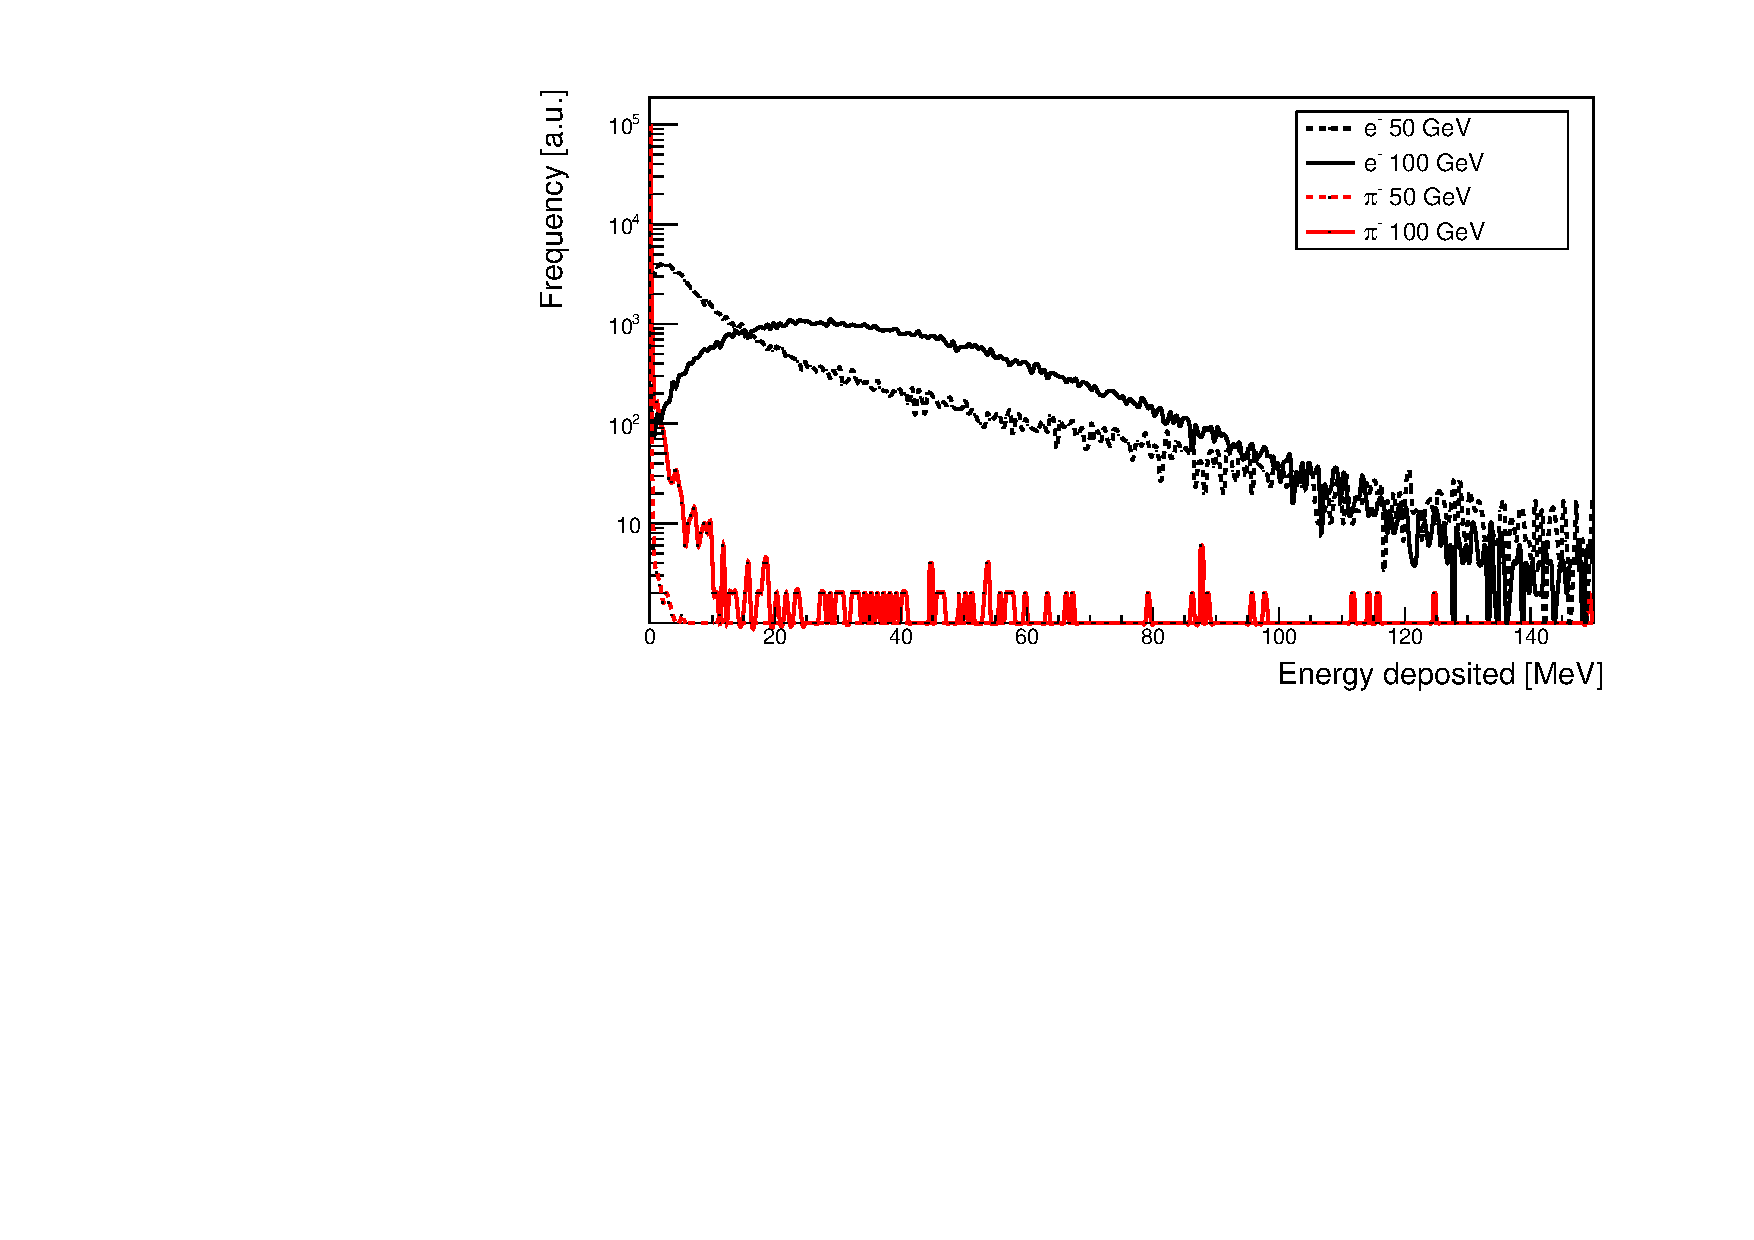
\includegraphics[width=1.\textwidth]{\pdirthree/comp_spectra.pdf}
\caption[SR spectrum for different energy detected in the SRD]{Result of the Geant 4 simulation for the energy detected by the SR detector for 50/100 GeV e$^-$(black dashed/solid line) and 50/100 GeV $\pi^-$ (red dashed/solid line).}
\label{fig:SRspectrum}
\end{figure}

The SRD detector was tested during the NA64 test beam run in July 2016. The two BGO rows are parallel to the primary beam direction as shown in Fig.\ref{fig:newgeo}. The dipole magnets installed in series produce a total integrated magnetic field of 7 \si{\tesla\meter} \cite{Banerjee:2016tad} resulting in a nominal displacement for the incoming electrons at the SRD/ECAL positions of 31/34 cm from the undeflected beam axis. The SRD was placed between the undeflected and the deflected beam axis at a distance of approximately 9 cm from both (Fig.\ref{fig:newgeo}). This separation minimises the possibility for Bremsstrahlung photons and neutral particles produced by interactions of the beam particle with materials upstream and for particles in the beam halo to hit the SRD. In fact, such interactions result in the saturation of the SRD with a significant loss of efficiency due to the long decay time of the BGOs.

%The expected Landau distribution of energy deposits was fit to the data to find the mean peak position to extract the calibration constant. 

The two crystals facing the beam (labeled 3 and 7 in Fig. \ref{fig:newgeo}) detect most of the energy emitted by synchrotron radiation. We will refer to those as SRD BGO. The remaining six crystals are used to detect events with high energy deposition in the SRD. In particular the last two crystals of each row (labeled 0 and 4 in Fig. \ref{fig:newgeo}) detect some energy only in the case of very energetic Bremsstrahlung events and thus can be used as a veto (see Fig.\ref{fig:newgeo}). The six crystals after the SRD BGOs act also as a shield from backscattering particles coming from the ECAL suppressing pions by an additional order of magnitude. Finally in this geometry it is possible to use the coincidence of the two SRD BGO crystals to improve the tagging of synchrotron photons by rejecting knock-on electrons produced by incoming pions. In fact synchrotron radiation has a homogenous spectrum in the whole arc described by the primary and deflected beam and thus a signal is detected in both SRD BGO. On the contrary, electrons generated by a $\pi^-$ undergoing ionisation will mostly leave energy only in a single crystal as illustrated in Fig. \ref{fig:newgeo}. 
With the requirement of detecting in both SRD BGOs an energy deposition above a 1 MeV the suppression factor is improved up to a level of $10^{-5}$.



\begin{figure}[htb!]
  \centering
  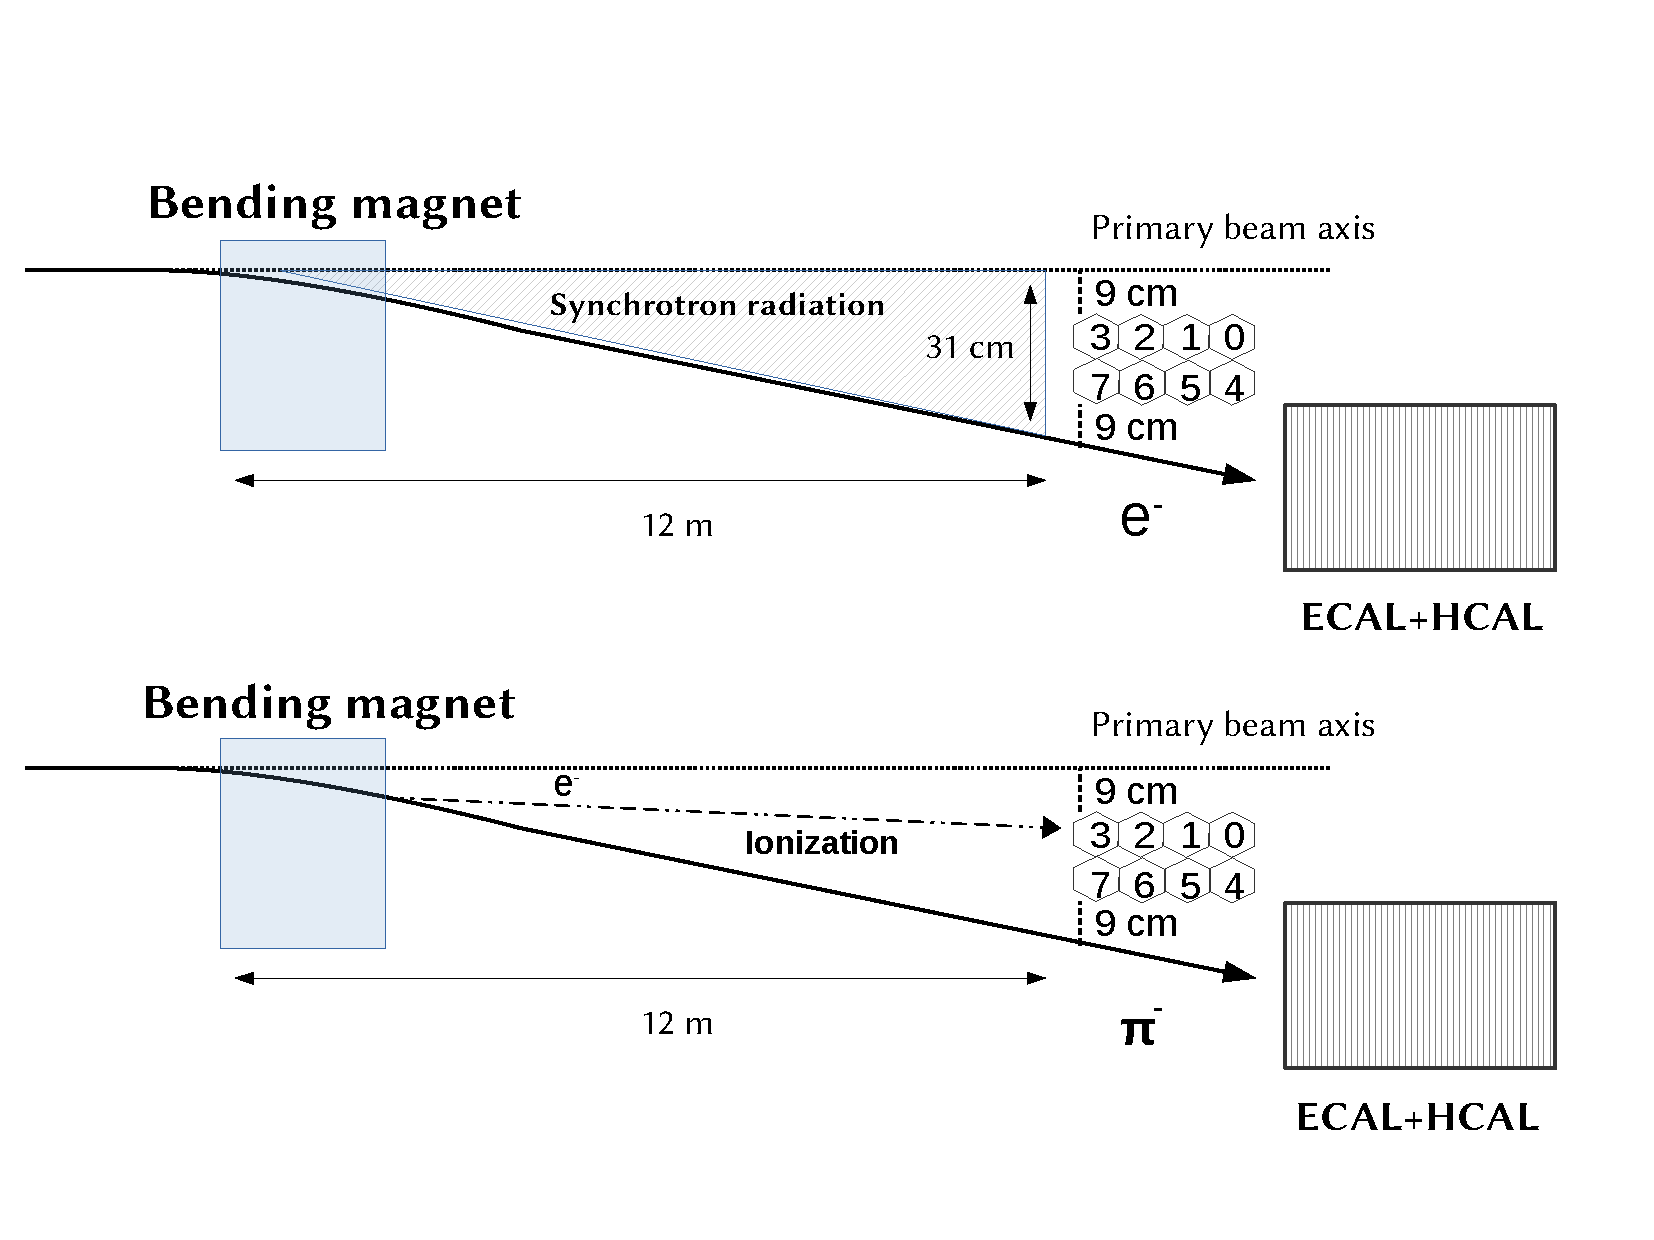
\includegraphics[width=.9\textwidth]{\pdirthree/sketch.pdf}
  \caption[Geometry of the BGO crystals]{Geometry of the BGO crystals. Crystals 7,3 (SRD BGO) collect most of the synchrotron radiation spectrum. Crystals 4,0 (VETO BGO) on the other hand are effected only in case of a high energy event and are thus used as a veto. The remaining crystals serve as a shield for the SRD from backscattering particles coming from the ECAL. Top: illustration of event leaving a SR signal in the SRD. Bottom: illustration of a SR- like signal in the SRD for a knock-on electron produced by pions.}
\label{fig:newgeo}
\end{figure}

Data with a 100 GeV $\pi^-$ beam were taken to have a direct measurement of the suppression factor achievable through synchrotron radiation measurements. The beam intensity was 5.3$\times 10^4$ particles per spill. The trigger was given by the coincidence of the three plastic scintillator counters (S1, S2 and S3 shown in Fig.\ref{fig:setup-invis-2018}). The additional requirement of an energy deposition below 60 GeV in the ECAL was applied in order to completely reject electrons from the $\pi^-$ sample of $\sim 10^5$ collected events.

For the 100 GeV electron beam run, a total of 220 spills were recorded with an intensity of 3.4$\times 10^5$/spill. 
The same trigger used in the pion run was used for the electron data.
In this case though, in order to reduce the pion contamination which is at a level of few \% and obtain a pure sample of electrons-only events with a total energy deposition in ECAL + HCAL above 90 GeV but with less than 20 GeV energy in the HCAL were used.  


The energy spectra recorded by the SRD BGO with electrons and pions are shown in Fig.\ref{fig:comp_spectra}. The SR spectra obtained with the electron beam are used to perform the BGO calibration by comparison with the simulation. With this method a very good agreement of data and MC is achieved (see plot on the left of Fig.\ref{fig:comp_spectra}). As a cross check, using the obtained calibration constants, the data from the pion beam impinging directly on the SRD are fitted with a Landau distribution. The obtained peak position of 60 MeV is in good agreement with the prediction of the MC. 

Time coincidence of signals above the energy threshold of 1 MeV from both SRD counters is required and high energy Bremsstrahlung events are removed using the veto BGO.
The suppression of synchrotron radiation emission detected for pions compared to electrons is clearly visible by comparing the two plots. For the electron spectrum, a 1\% pileup beam events have been added to the simulation as predicted for the given spill intensity and with the known decay time of BGOs.  Both spectra are in very good agreement with the simulation.

\begin{figure}[htb!]
  \centering
  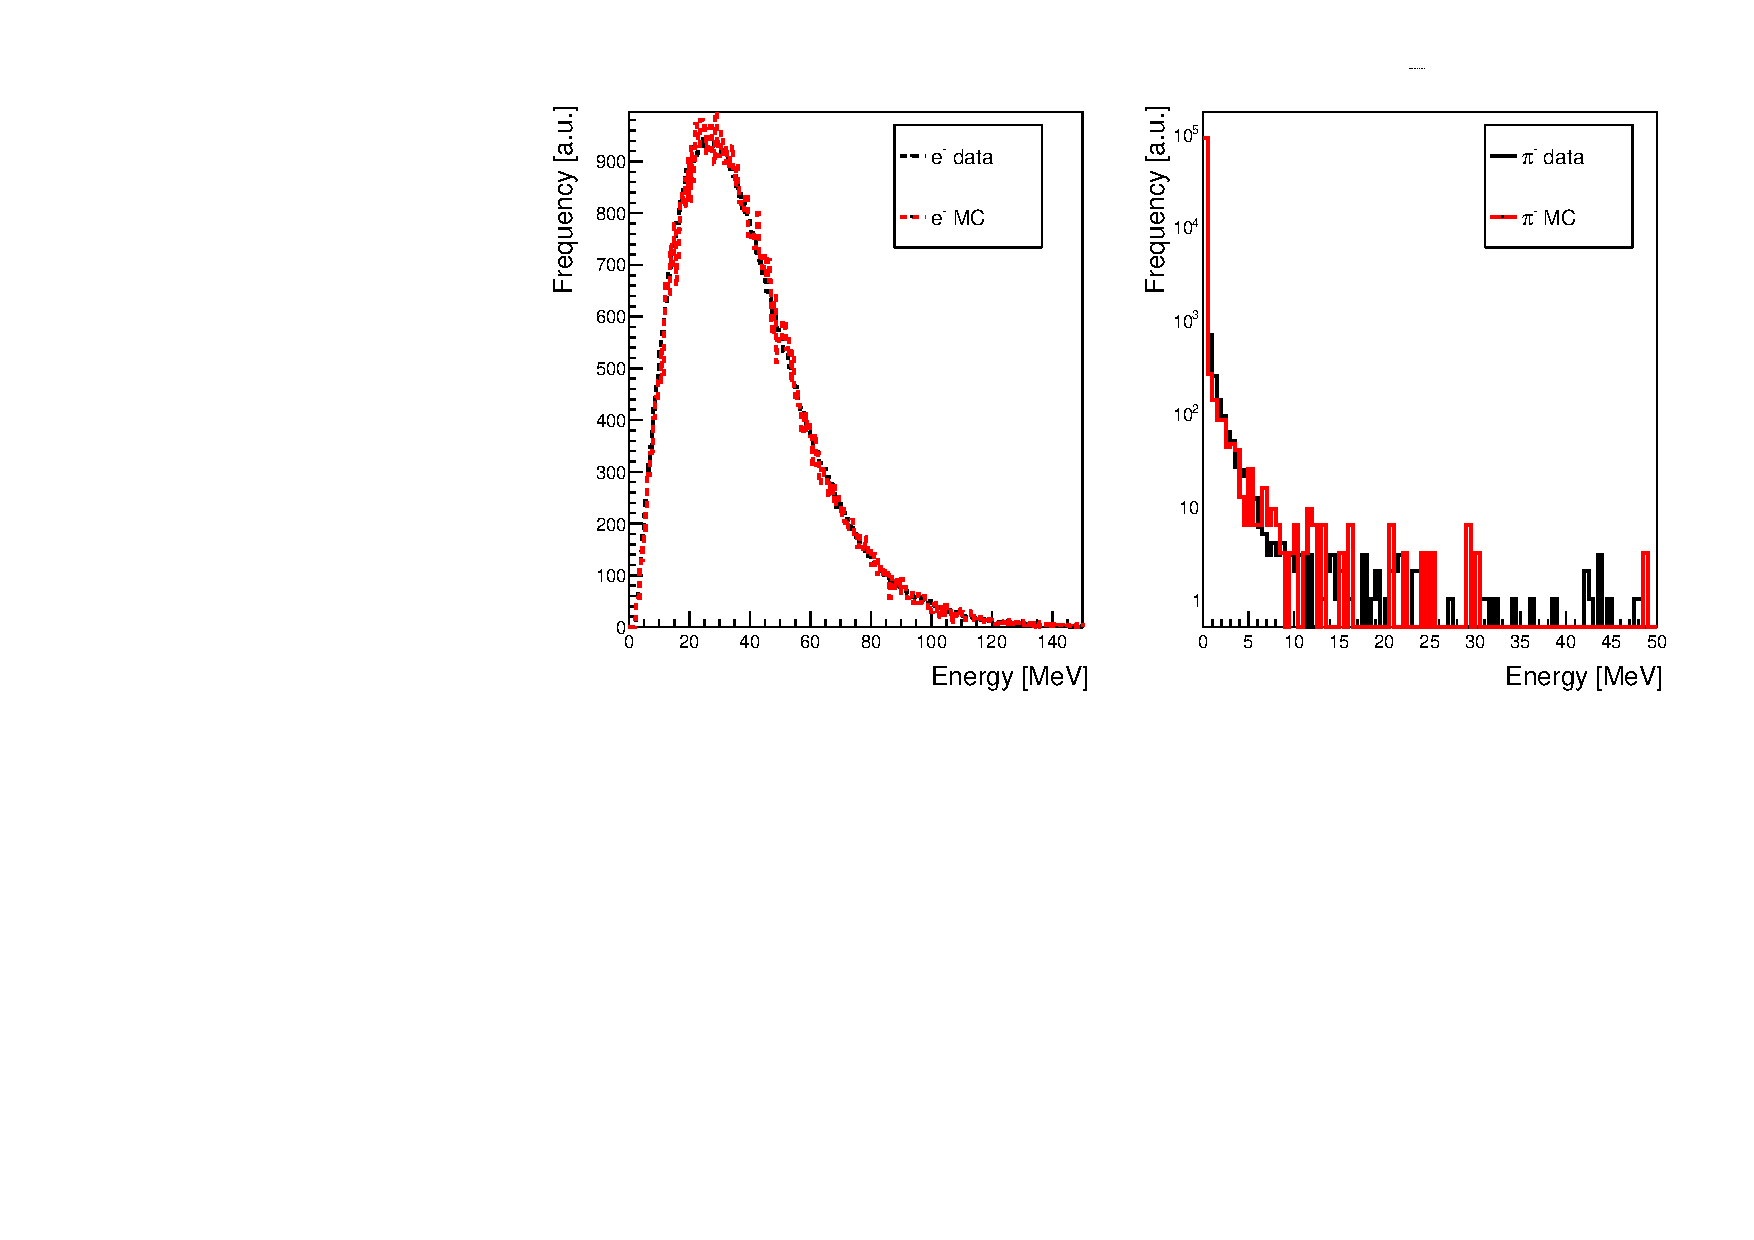
\includegraphics[width=1.\textwidth]{\pdirthree/spectra_tot.pdf}
  \caption[SRD comparison between data and MC]{Comparison between data and simulation (MC) of the synchrotron radiation spectrum detected for 100 GeV electrons (left) and pions (right). }
  \label{fig:comp_spectra}
\end{figure} 

\begin{figure}[htb!]
  \centering
  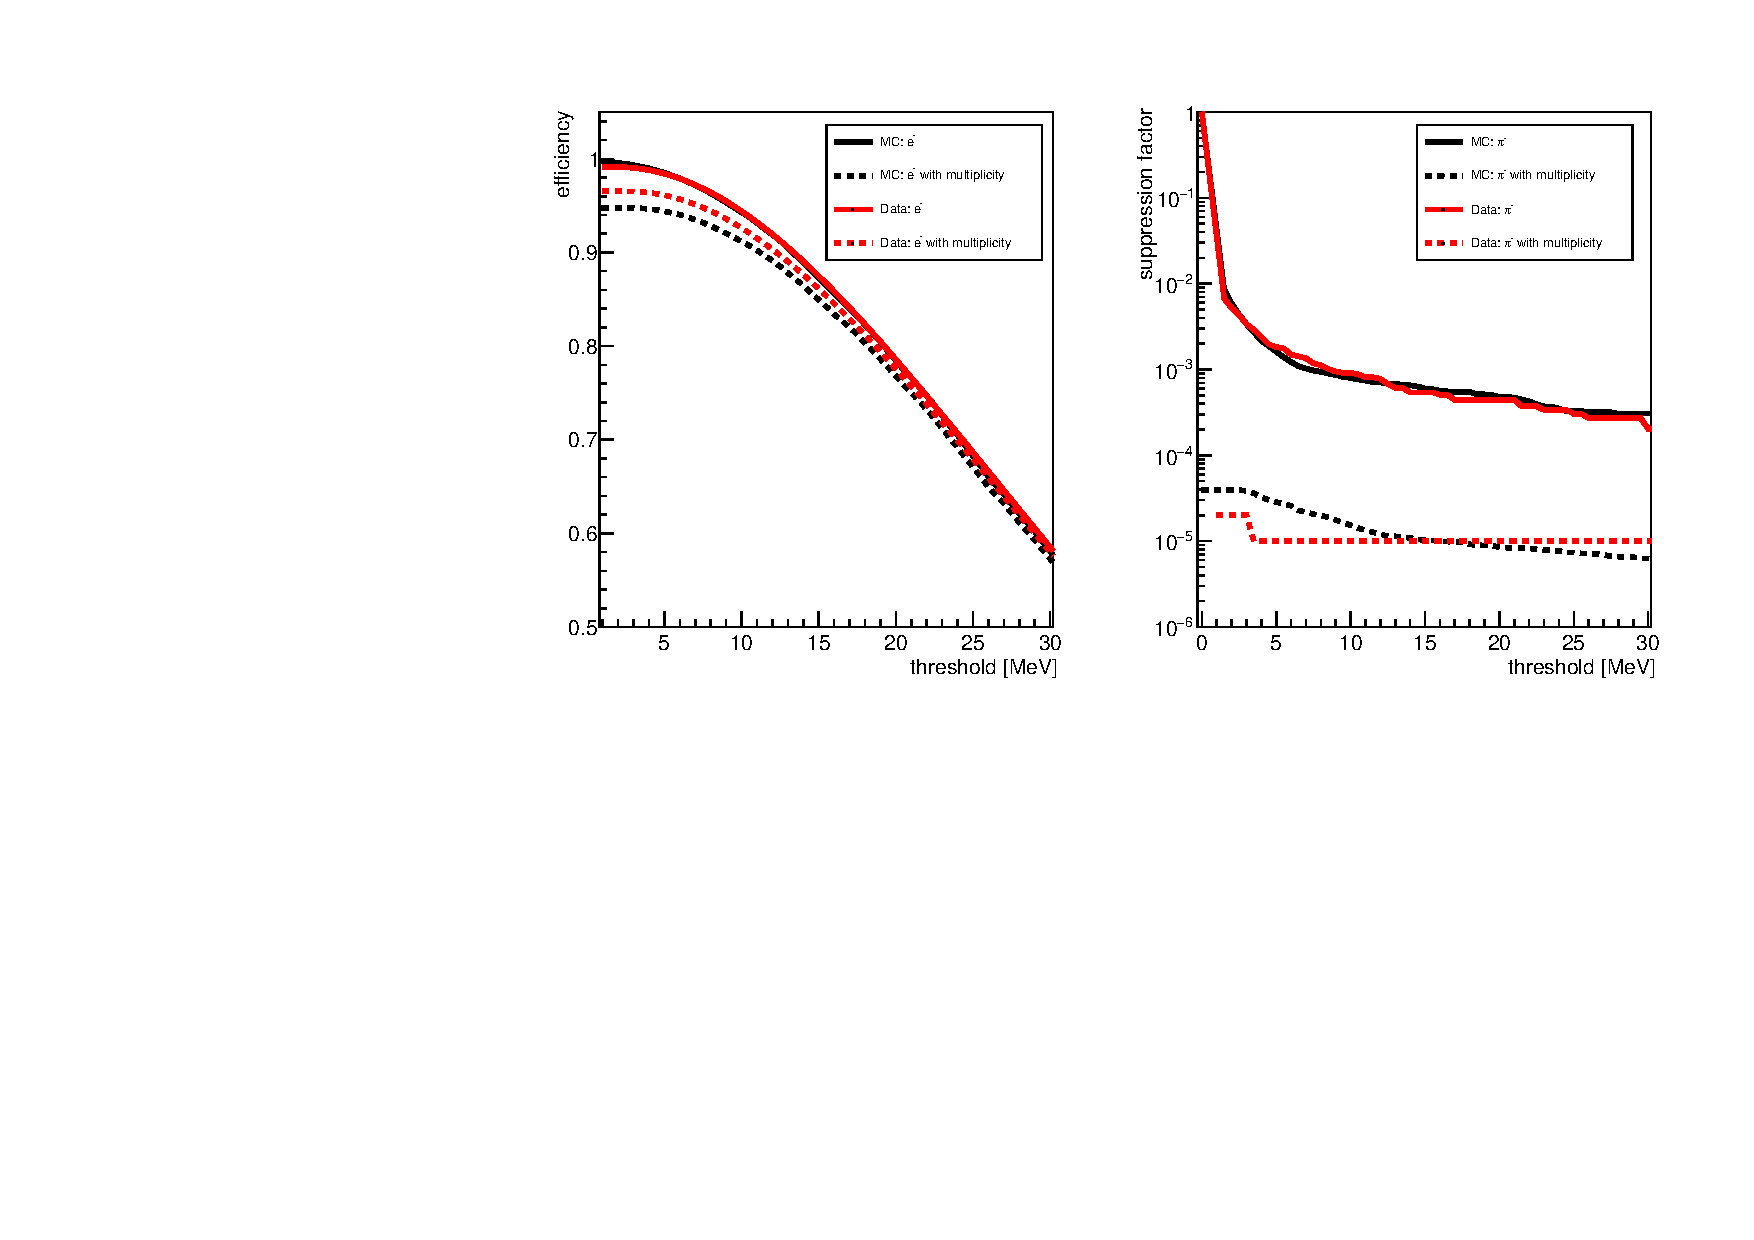
\includegraphics[width=1.\textwidth]{\pdirthree/sup_mult.pdf}
  \caption[efficiency and rejection power of the SRD cut]{Left: Comparison between data and simulation (MC) for electrons of the efficiency as a function of threshold set on the total energy deposited in the SRD BGO and for the requirement that this is deposited in each single crystal (multiplicity). Right: Comparison between data and simulation for pions and electrons of the suppression factor as a function of the threshold set on the total energy deposited in the SRD BGO and for the multiplicity requirement.}
  \label{fig:sup_mult}
\end{figure}

The efficiency for the electrons and the suppression factor for the pions are plotted in Fig. \ref{fig:sup_mult} as a function of the threshold on the energy deposited in the SRD. We distinguish between two cases:
\begin{enumerate}
\item The threshold is set on the total energy deposited in the SRD.
\item Both SRD signals have to be in-time and above the threshold of 1 MeV (multiplicity requirement).
\end{enumerate}
One can see that applying the criterion 2) the efficiency only decreases slightly compared to 1), while the suppression factor for pions is dramatically increased (by two orders of magnitude) with the requirement of having the two BGOs in coincidence.
This can be understood because the SR-like signal generated from secondary electron will leave a signal only in one of the two BGOs while the SR from electrons is spread out uniformly as explained above. 
This is also underlined by Table  \ref{tab:hits} where the fraction of events with different hit multiplicity in the SRD BGO for both pion and electron runs are reported.

\begin{table}[hbt!]
\begin{center}
\begin{tabular}{cccc}
Events hit multiplicity  (\%) & 0 BGO  & 1 BGO & 2 BGOs\\
\hline
Pions & $98.77$ & $1.21$ & $1.4\times10^{-3}$  \\
Electrons & $2.4\times10^{-1}$  & $2.60$ & $97.37$ \\
\end{tabular}
\end{center}
\caption[Fraction of pion and electron events for different hit multiplicity in the SRD from the data]{Fraction of pion and electron events for different hit multiplicity in the SRD from the data.}
\label{tab:hits}

\end{table}

\subsection{Hadron rejection using electromagnetic shower profile}
\label{ch3:sec:bkg-ecal-profile}

On the top of rejection using SRD, the transversal segmentation of the ECAL offers another tools for hadron rejection. The idea is to discriminate between a classical em-shower profile to a more complex hadronic shower using a $\chi^2$-test. A shower profile database can be built by correlating the hit position (x,y) on the ECAL with the fraction of energy deposited in each ECAL cell. The method used to build this database is detailed in Appendix.\ref{Appb:sec:make_profile}. A predicted value of energy deposited in each ECAL cell is extracted and compared to the one measured in the event. The compatibility between the predicted profile and the measured one can be tested using the $\chi^2$-distribution:

\begin{equation}
  \chi^2 = \sum^{9,36}_i \left(\frac{E_{pred}^i(x_{hit},y_{hit})-E_{mes}^i}{\sigma^{i}_{pred}(x_{hit},y_{hit})}\right)^2
  \label{eqn:chi}
\end{equation}


\begin{description}
\item[$E_{pred}^i$]: is the energy predicted by the profile of cell
  $i$
\item[$E_{mes}^i$]: is the energy measured in the cell $i$
\item[$x_{hit},y_{hit}$]: coordinates of the hit position of the
  particle in the ECAL plane
\item [$\sigma^{i}_{pred}$]: error estimated for the predicted energy
  in cell $i$
\end{description}


Two different summation indexes are used for the two different cases
where only the cells surrounding the central one hit by the beam are
used for the test (total of 9 cells) and the case where all the cells
are used (total of 36, see Fig.\ref{fig:ecal_example}).

\begin{figure}[h!]
  \begin{center}
    \includegraphics[scale=0.47,page=4]{\pdirthree/ecal_example.pdf}
  \end{center}
  \caption[ECAL sketch]{sketch of the 36 cells of the ECAL. The central cell 3X3
    were the beam is directed is plotted in red, while the cells
    surrounding it are plotted in green. On the bottom-right an
    example of how a profile for a cell looks like in the MC.}
  \label{fig:ecal_example}
\end{figure}

To test the rejection power and the efficiency of the
method the algorithm described above was used for 3 type of samples\footnote{The database was generated using the electron  calibration runs 2363, 2182, 2410, 2406, 2438. A complete description of such runs can be found in \cite{na64-runs}. }:
\begin{itemize}
\item $\simeq$1.2$\times 10^{6}$ events acquired with an electron calibration run\footnote{run 2363}.
\item $\simeq$5$\times 10^{5}$ events acquired with an hadron calibration run\footnote{run 2204}.
\item $\simeq$8$\times 10^{5}$ events acquired using physical trigger at maximum H4 beam intensity.\footnote{run 2241, corresponding EOT before trigger suppression $\simeq 4 \times 10^{8}$}
\end{itemize}

The comparison of the normalized $\chi^2$-distribution between
electron calibration run and hadron run using information from all 36
cells is shown in Fig.\ref{fig:chi2}. Note that electrons reproduce
the expected shape of a $\chi^2$-distribution while for hadrons we
observe a displaced one incompatible with the one produced by
electrons.  The rejection and efficiency of a cut
$\chi^2 < \chi^2_{cut}$ are shown in detail in Fig.\ref{fig:eff}. For
a benchmark $\chi^2$-cut of 2 the efficiency calculated in run 2363
was $\sim 0.94$ with a rejection factor of $1.2\times 10^{-3}$
extracted from the hadron run 2204. These values as well as the ones
presented in Fig.\ref{fig:eff} are computed by looking at the total
number of events passing the cut and do not account for the impurities
in the beam.

Using information coming only from the 9 central
cells (Fig.\ref{fig:ecal_example}) appears to shift the distribution
to the left and reduce its spread ( Fig.\ref{fig:chi}) due to the
smaller number of degrees of freedom, the two methods have overall
comparable efficiency as can be seen in Fig.\ref{fig:eff} but smaller
rejection power when a typical cut is applied.  For the considered
benchmark cut of $\chi^2_{cut}=$2, the efficiency measured using only
central cells was of $\sim 0.93$\ and a rejection factor of
$3.1\times 10^{-3}$.


\begin{figure}[h!]
  \begin{center}
    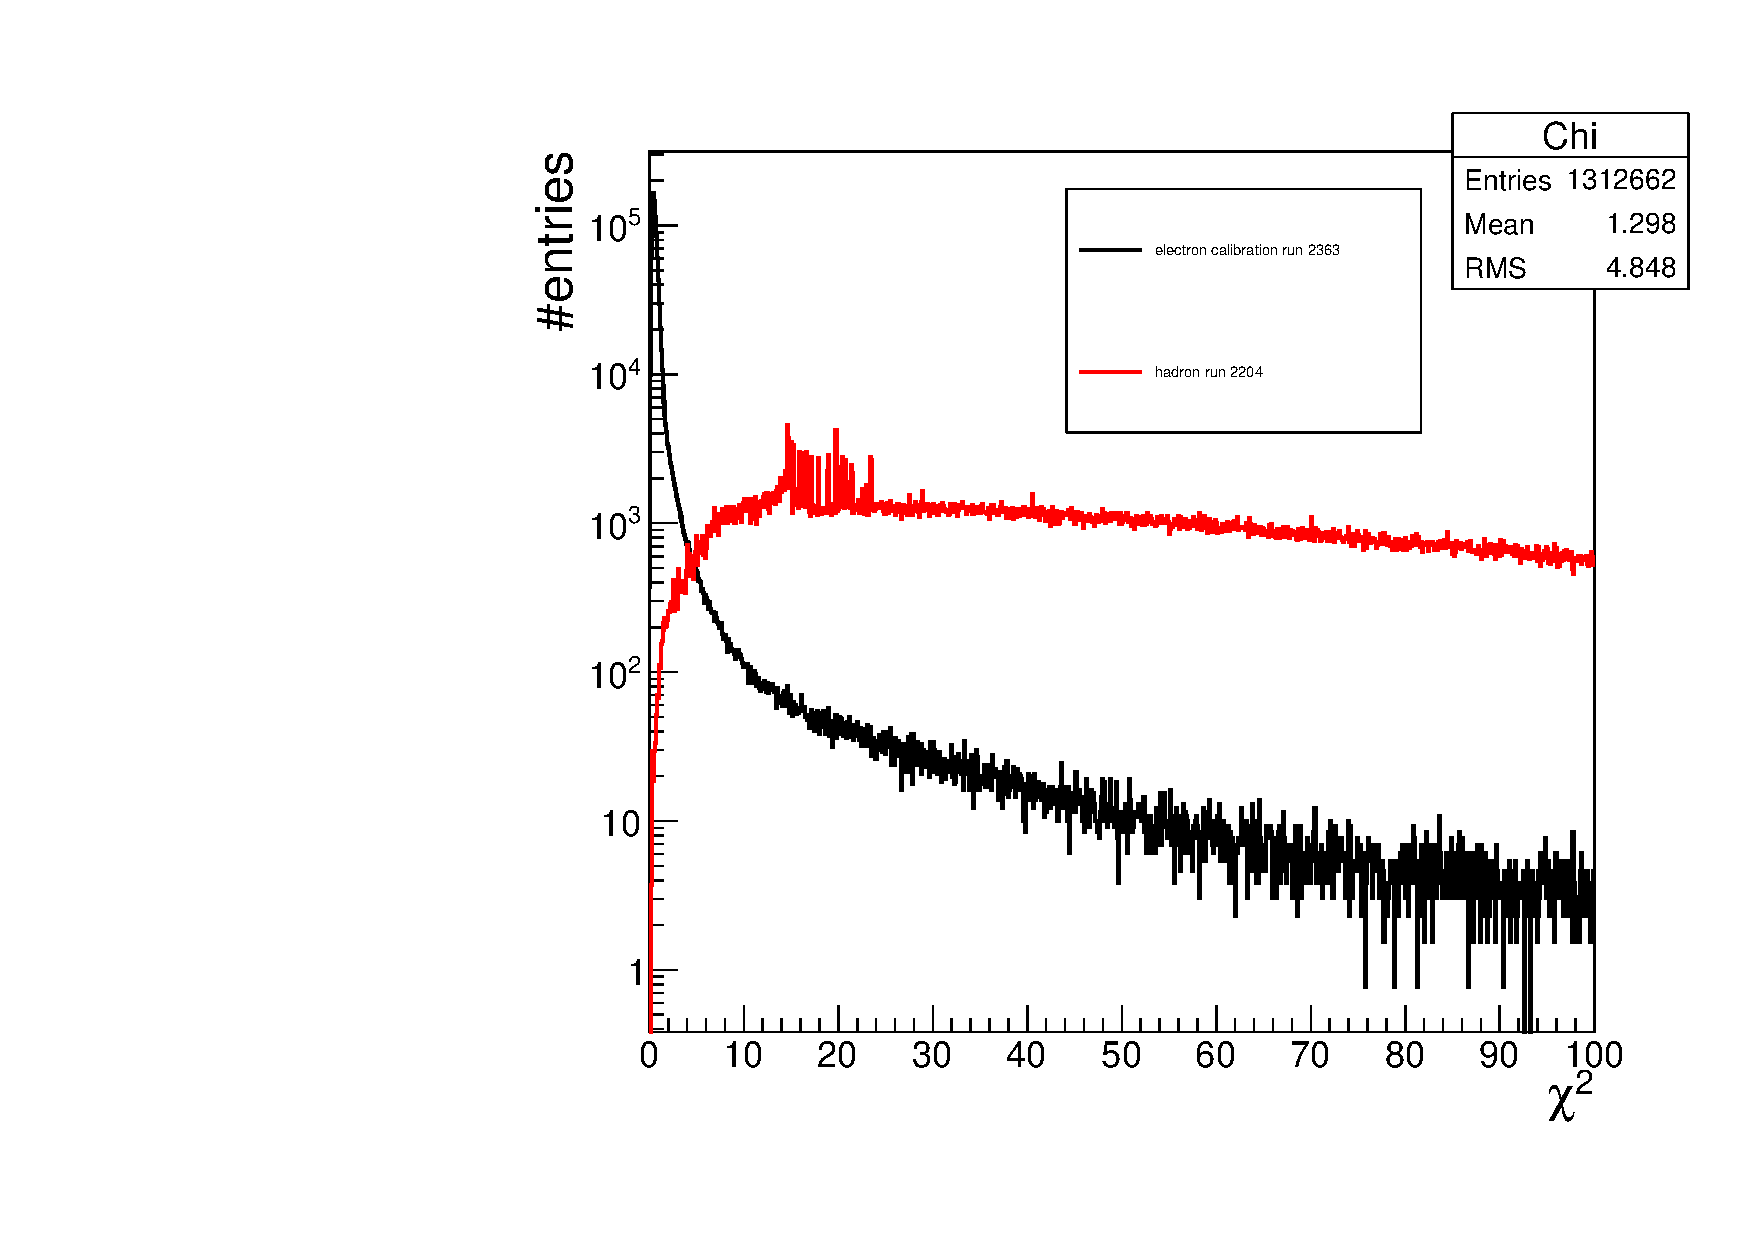
\includegraphics[width=0.95\textwidth,height=0.8\textwidth]{\pdirthree/chi_comp.pdf}
  \end{center}
  \caption[comparison between $\chi^2$ distribution, electron and hadron calibration run]{comparison between $\chi^2$ distribution generated from an electron calibration run (black) and hadron calibration run (red).}
  \label{fig:chi2}
\end{figure}

\begin{figure}[h!]
  \begin{center}
    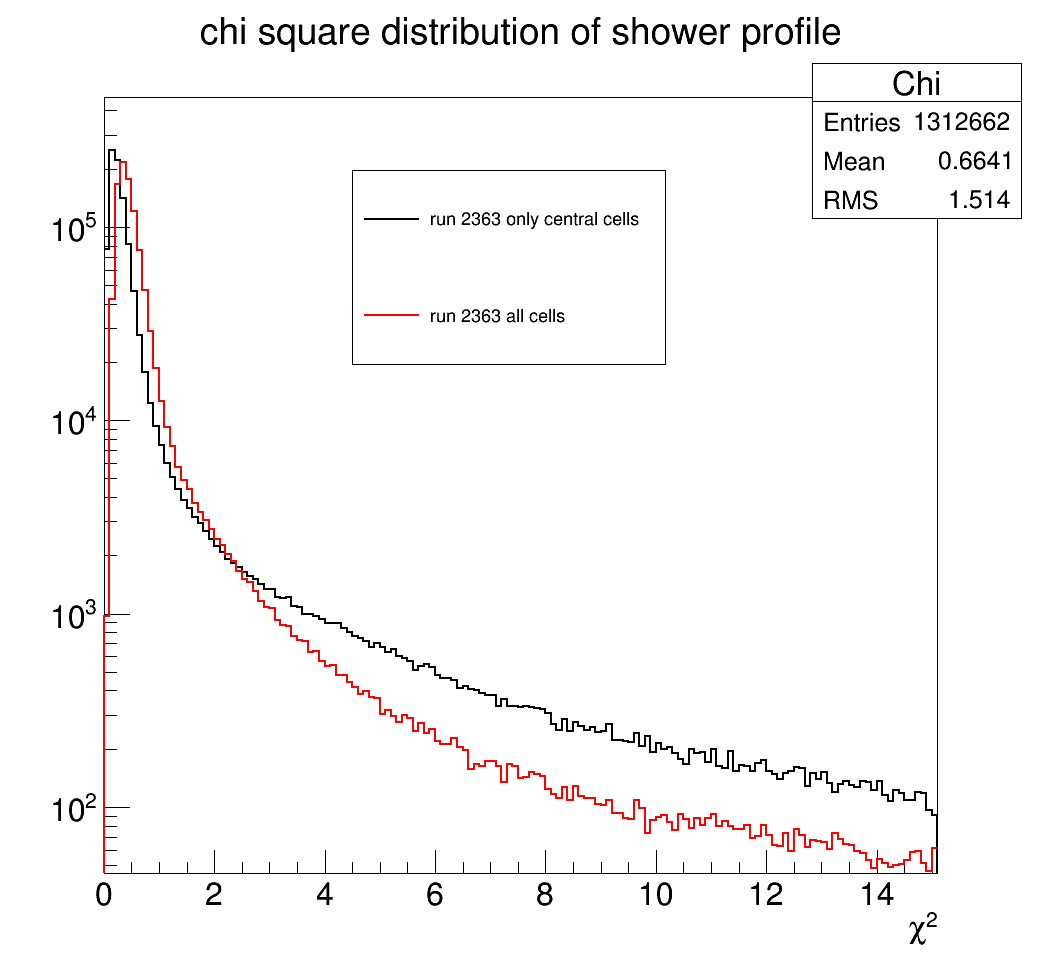
\includegraphics[width=0.95\textwidth,height=0.8\textwidth]{\pdirthree/plot_comp_cells.png}
  \end{center}
  \caption[comparison between $\chi^2$ distribution for different ECAL configurations]{comparison between $\chi^2$ distribution generated from an electron calibration run considering only central cells (black) and considering all 36 cells (red).}
  \label{fig:chi}
\end{figure}

\begin{figure}[h!]
  \begin{center}
    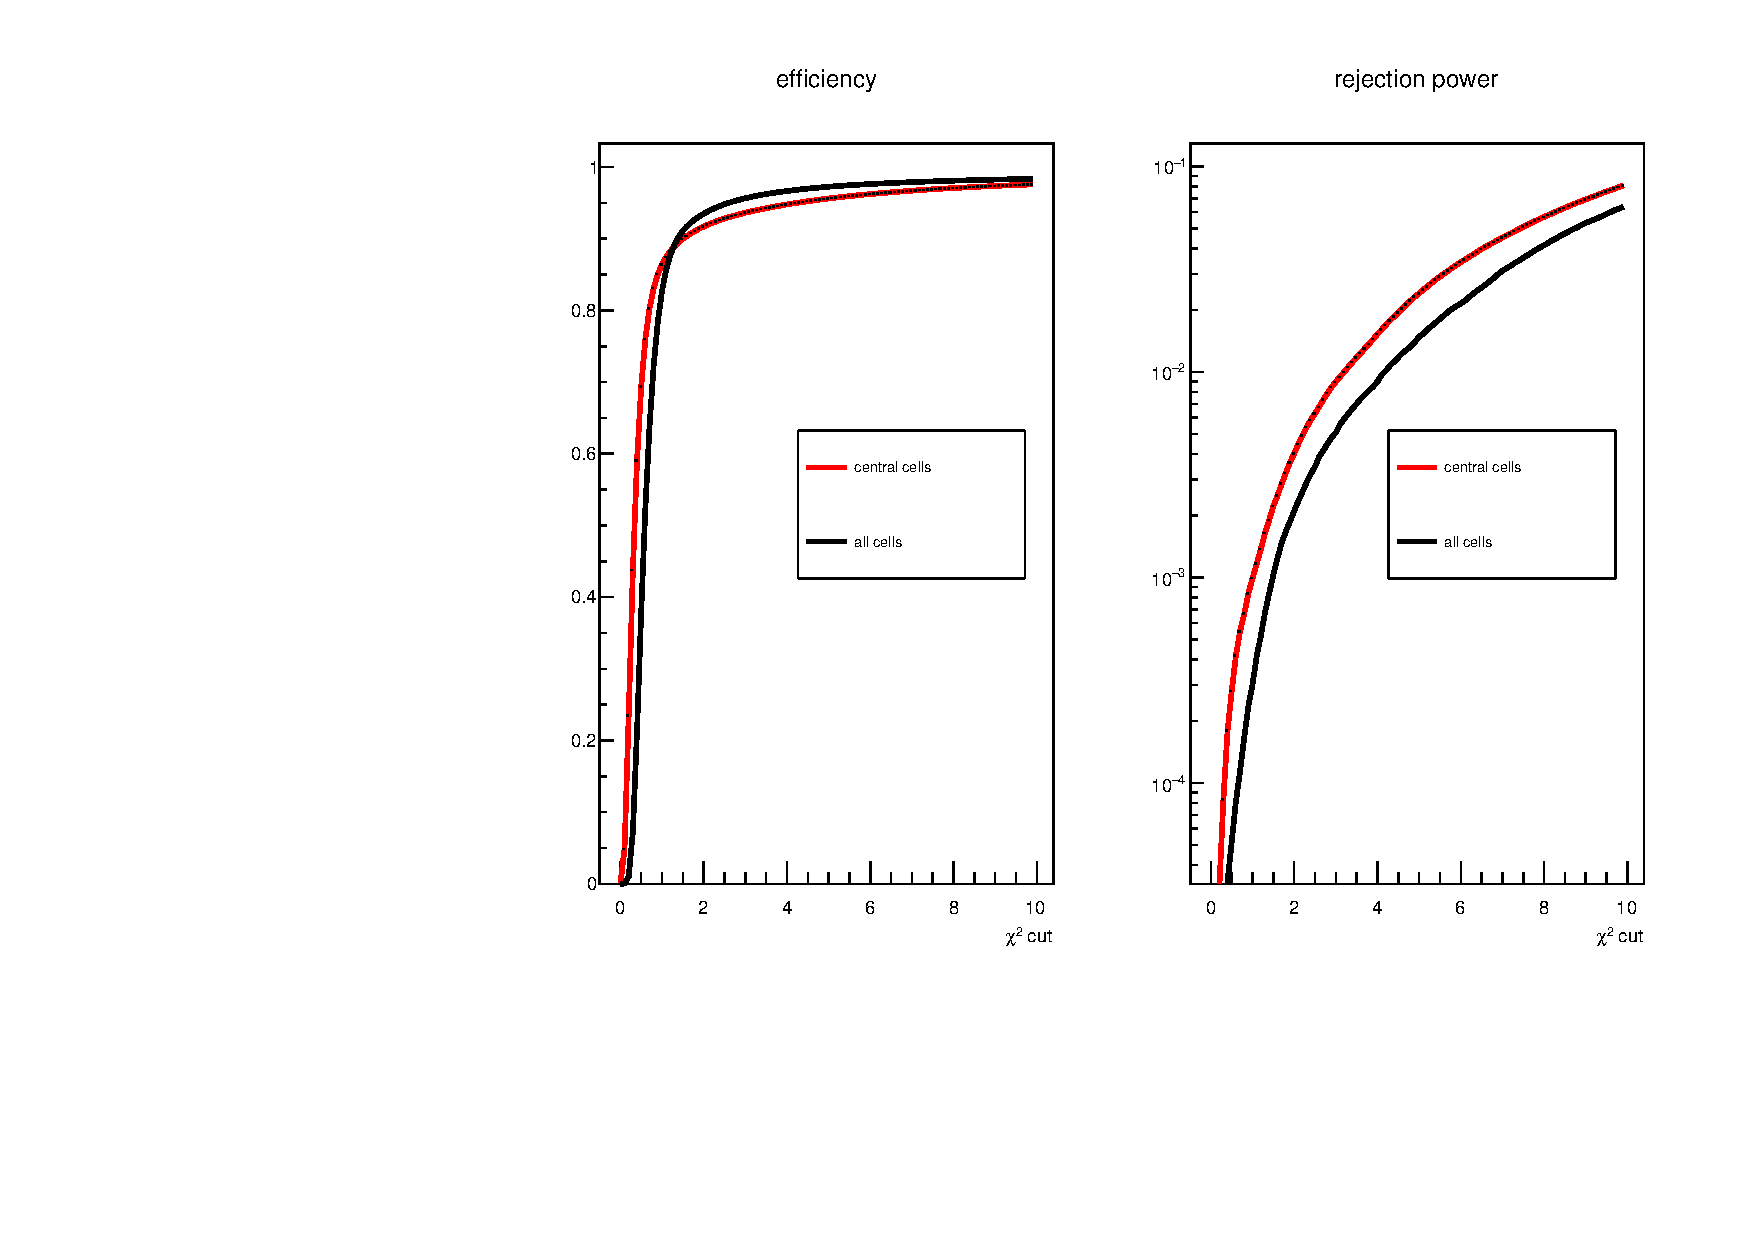
\includegraphics[width=0.95\textwidth,height=0.6\textwidth]{\pdirthree/eff.pdf}
  \end{center}
  \caption[fraction of events passing the $\chi^2$ cut]{fraction of events passing the cut $\chi^2 < \chi^2_{cut}$
    for the electron calibration run (left) and for the hadron calibration run (right).}
  \label{fig:eff}
\end{figure}

\clearpage

Different ECAL vs HCAL plots were produced to study the effect of a
$\chi^2$-cut for the run mentioned above. The one produced with
benchmark cut of $\chi^2 < 2$ are shown in
Fig.\ref{fig:ehcal_test}. The cut is shown to clean the plot in the
way expected from the hadronic activity in all selected runs. It can also
can be seen from the run recorded with physical trigger that events involving the dimuon
production $e^- \to \mu^+\mu^-$ survive the cut for energies larger
than 20 GeV.  This is expected since these events will still involve
an electromagnetic shower truncated in the moment the transition
happens. Since a possible signal from a Dark Photon would behave
similarly this suggest that the cut won't reject the signal provided
that the shower has enough energy. A similar study performed with the
MC reached the same conclusion, however for
very small energies the shower shape will slowly reach the energy
resolution in each cell and the efficiency of the cut will drop
substantially.  The efficiency for low energy improves if only central
cells are selected for the $\chi^2$ calculation since this will reduce
the fluctuation of the single cells not involved in the shower. This
effect is shown in Fig.\ref{fig:ehcal_comp} for a cut of 2 on $\chi^2$.
\\
\\
For low energy particles it is clear that all the shower will be
contained in the cell 3x3. Below this threshold shower analysis can no
longer resolve the type of shower of the event and instead the simple
requirement of the full energy of the event to be detected by the
central cell (3x3) should be used to avoid killing the
signal. Applying a $\chi^2$-cut to a dark photon simulation suggested that this limit is roughly 5 GeV.  The
left plot in Fig.\ref{fig:ehcal_comp} is compatible with this
estimate.


\newpage
\begin{figure}[h!]
  \begin{center}
    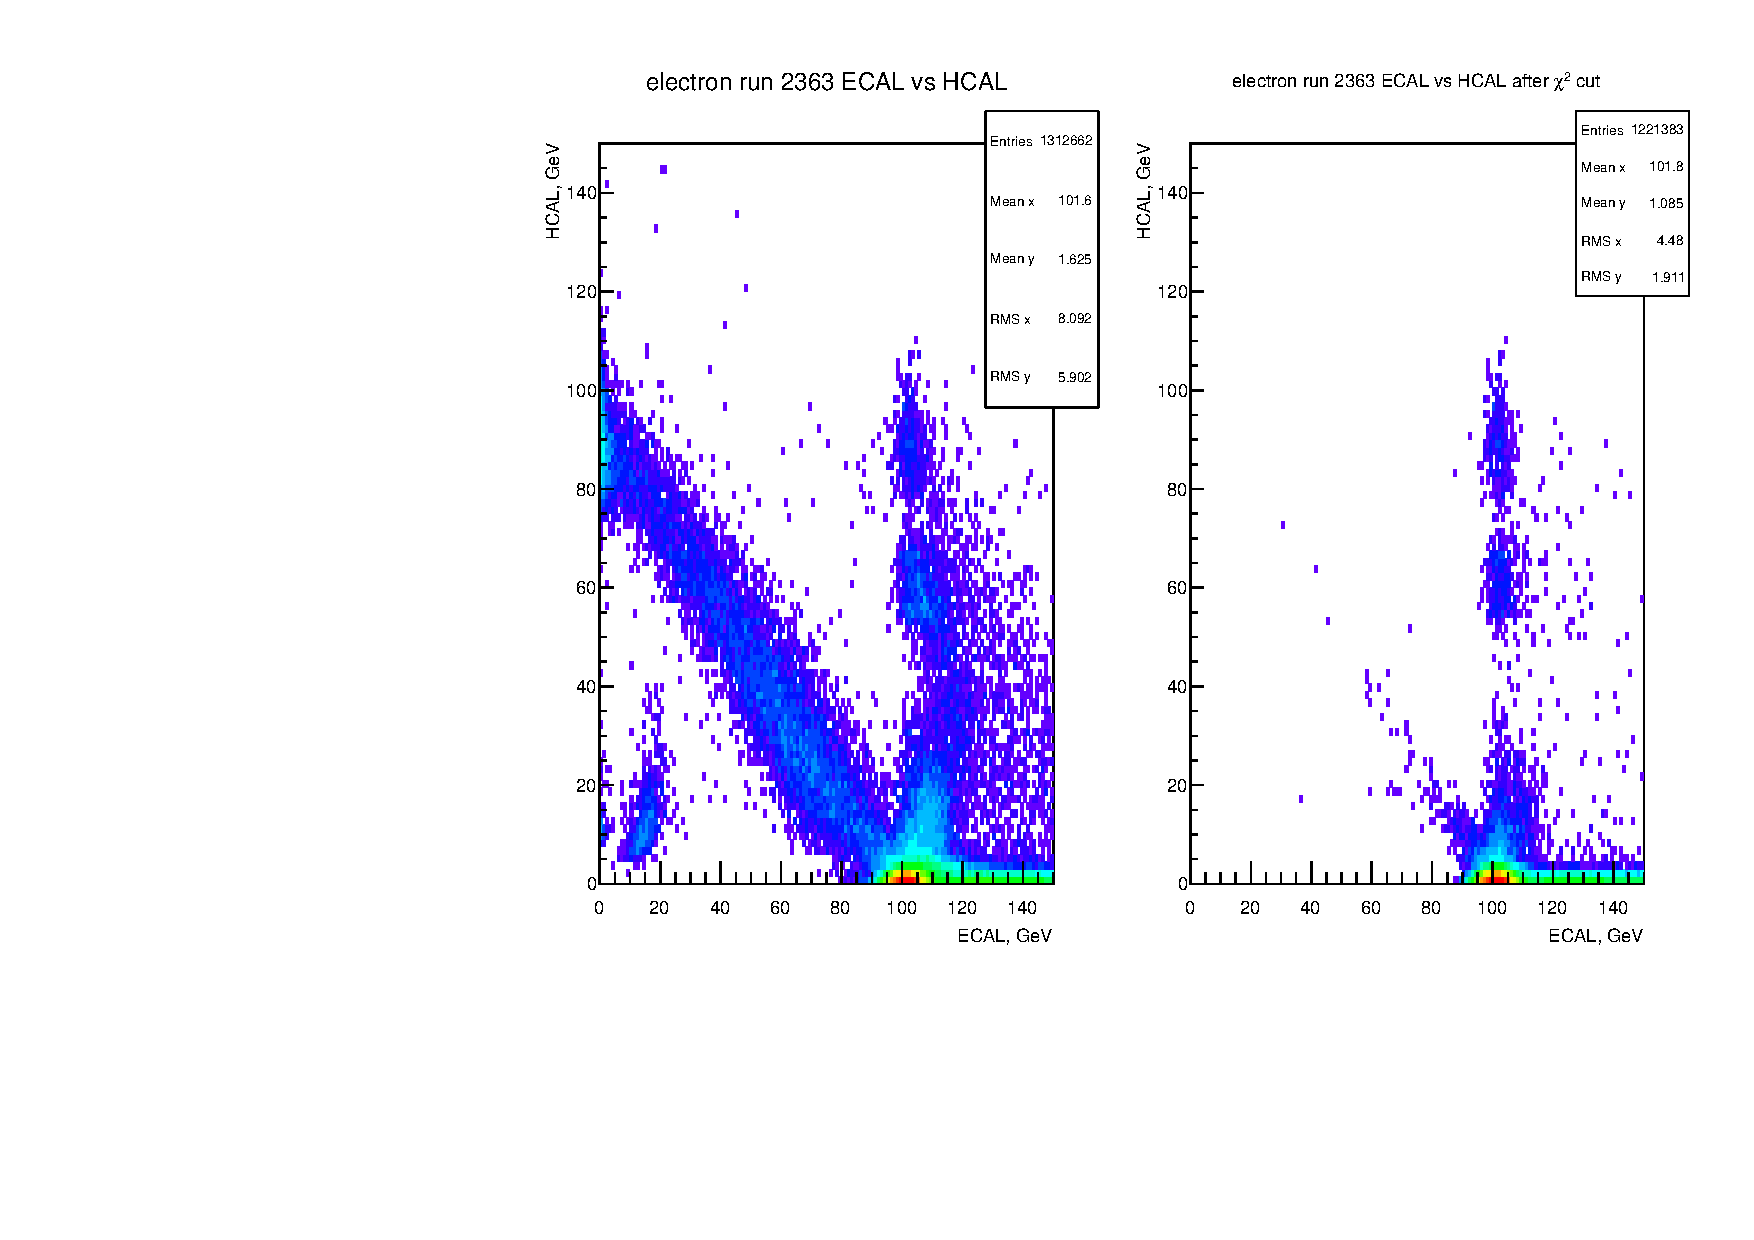
\includegraphics[width=0.95\textwidth,height=0.45\textwidth]{\pdirthree/ehcal_2336_chi.pdf}
    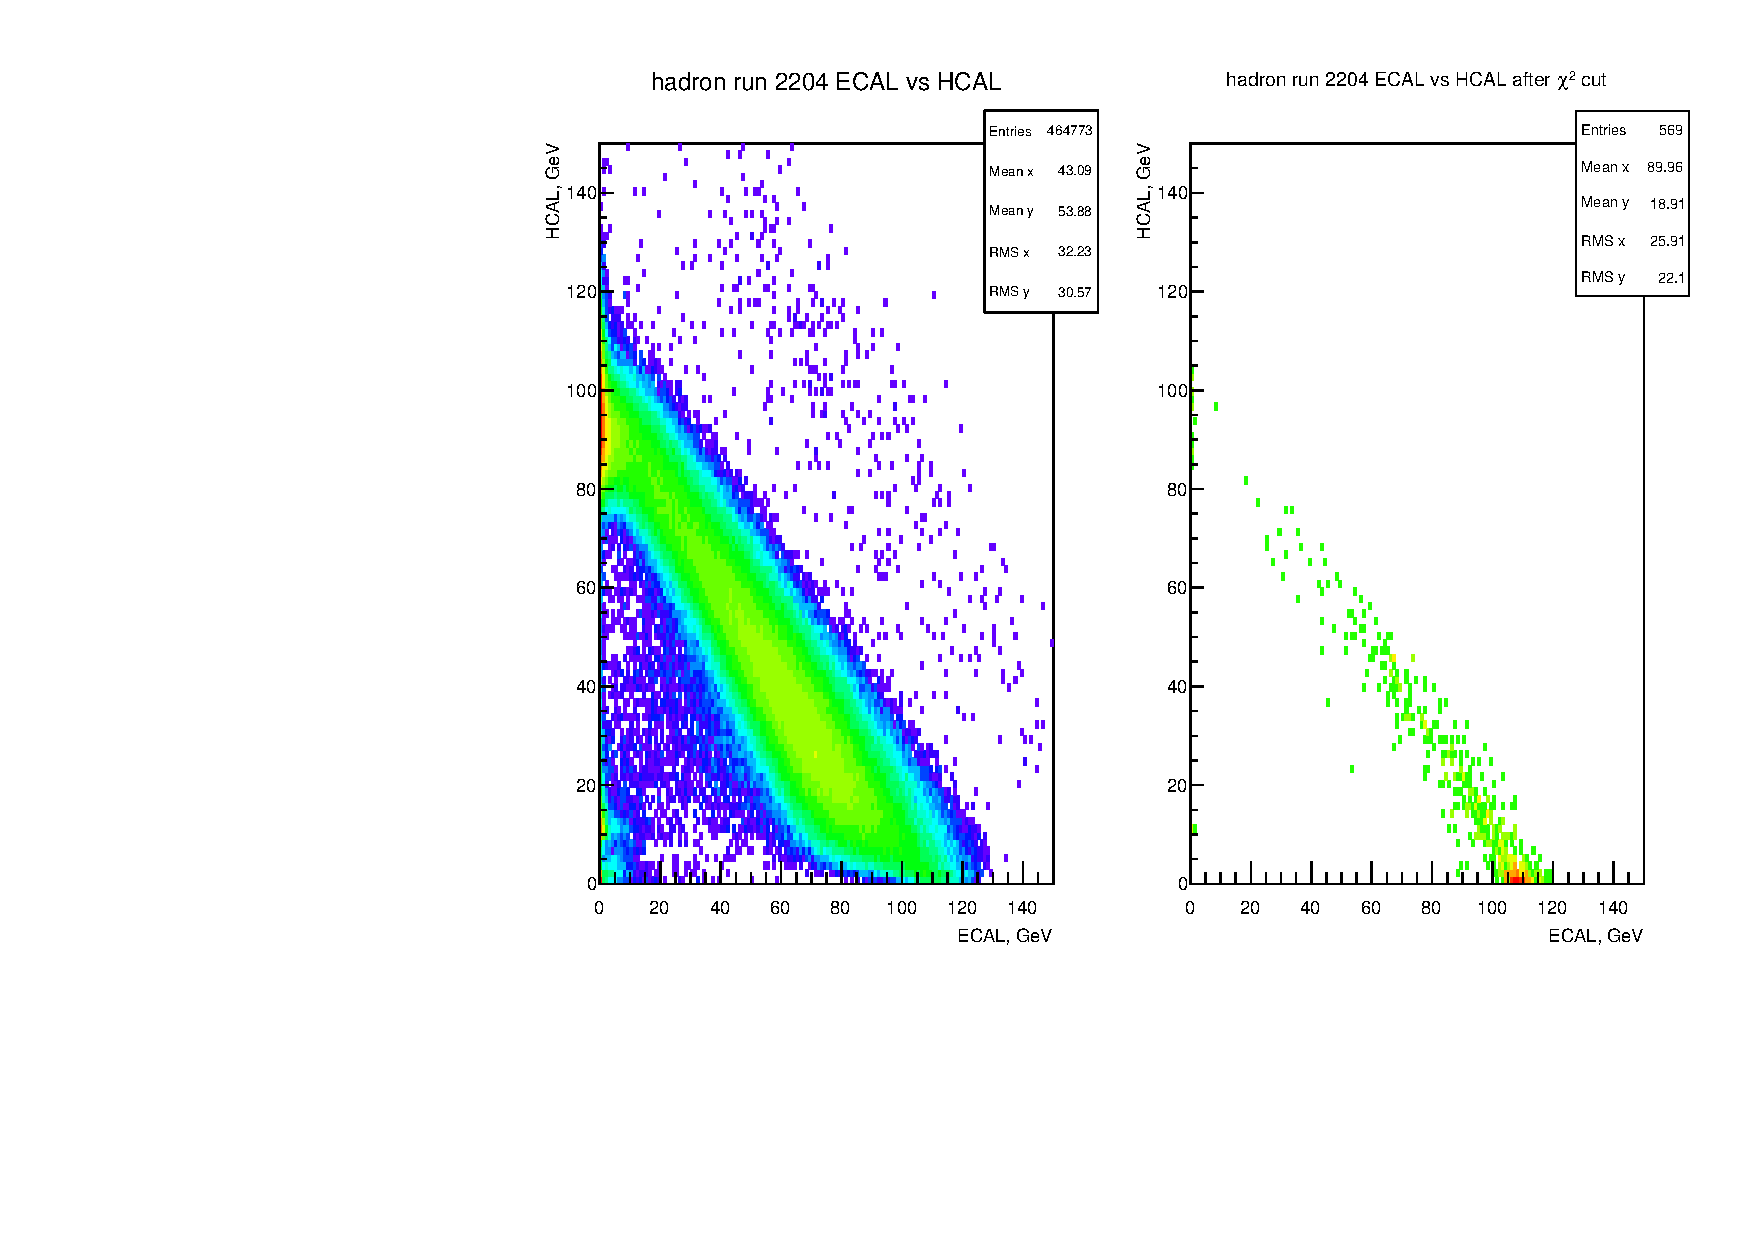
\includegraphics[width=0.95\textwidth,height=0.45\textwidth]{\pdirthree/ehcal_2204_chi.pdf}
    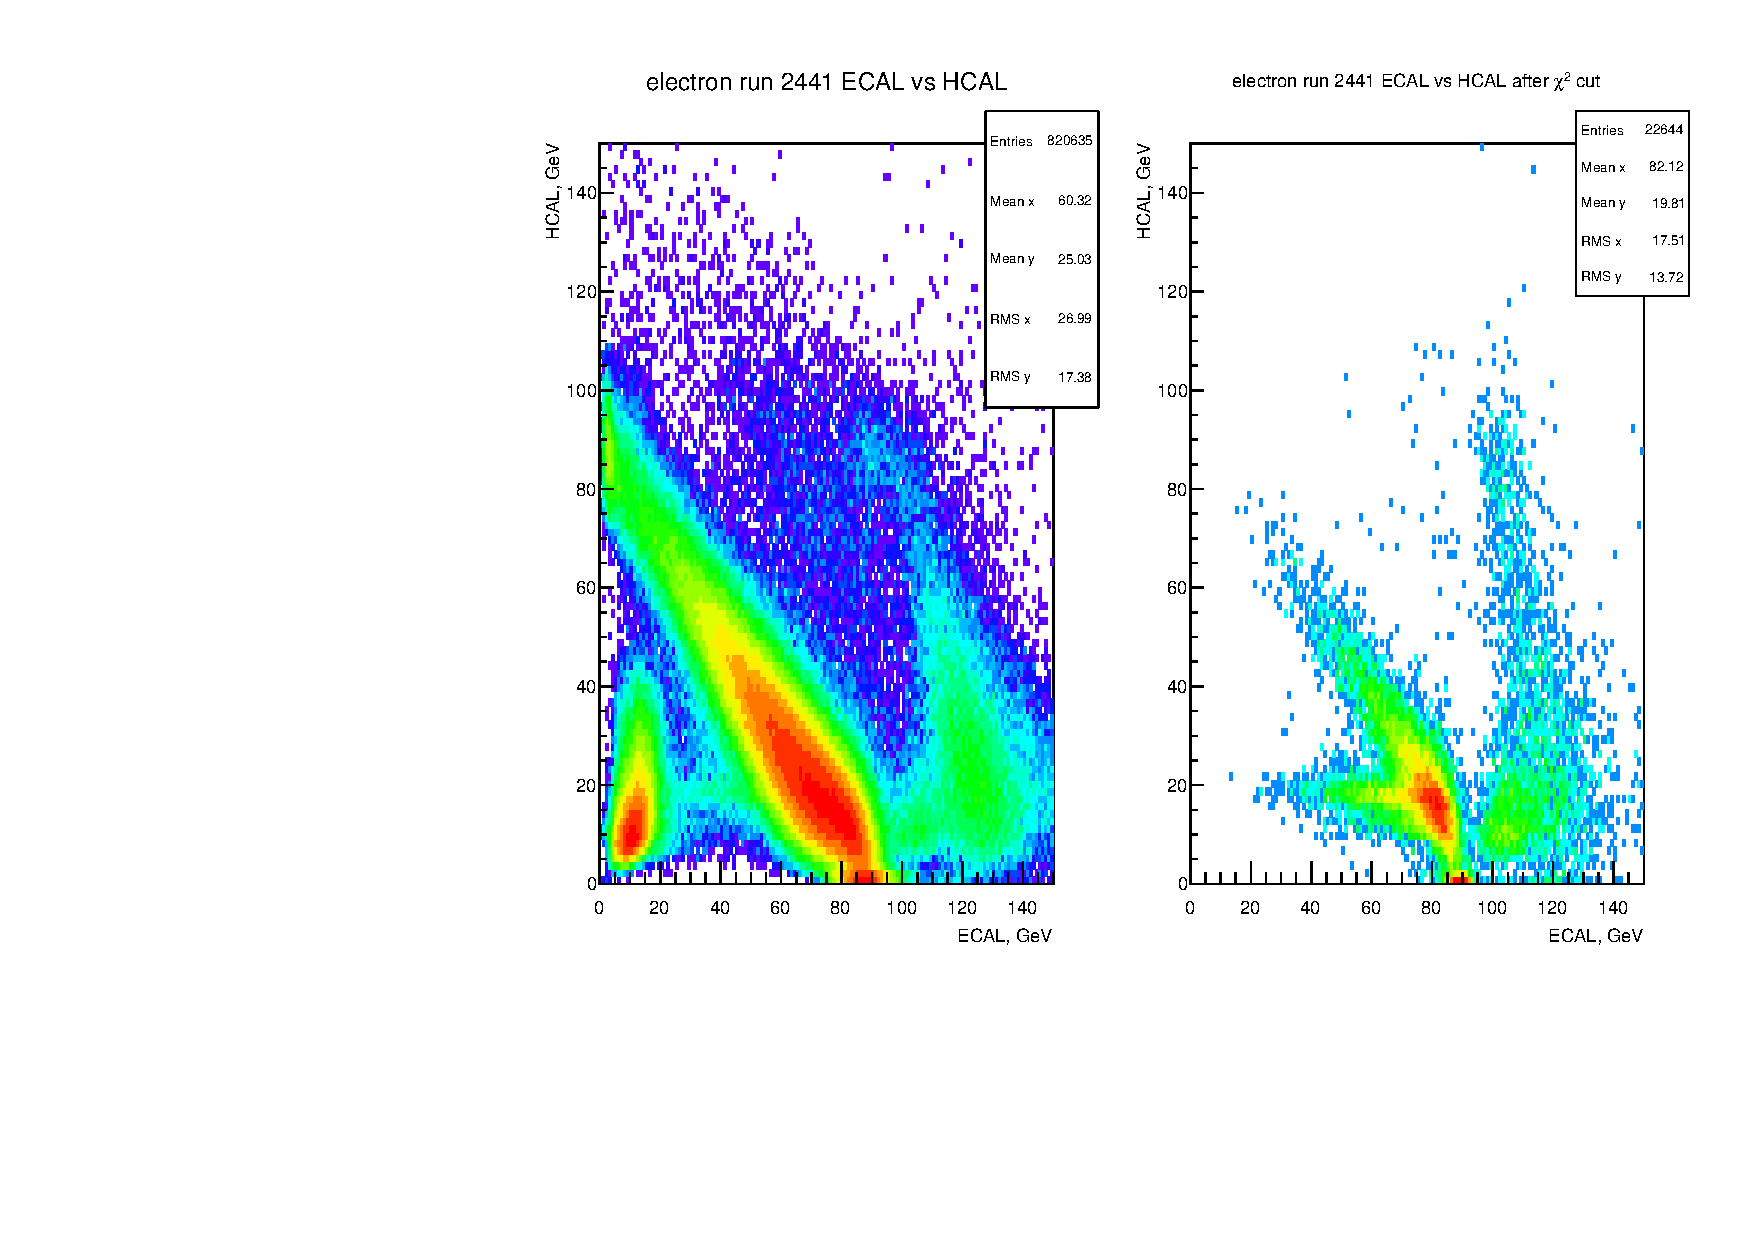
\includegraphics[width=0.95\textwidth,height=0.45\textwidth]{\pdirthree/ehcal_2441_chi.pdf}
  \end{center}
  \caption[ECAL vs HCAL energy deposit after a cut $\chi^2$]{ECAL vs HCAL energy deposit for the total sample (left
    column) and after a cut $\chi^2<2$ (right column) for the
    electron calibration run (top), the hadron calibration run (middle) and the run recorded with physical trigger(bottom).}
  \label{fig:ehcal_test}
\end{figure}
\clearpage

\begin{figure}[h!]
  \begin{center}
    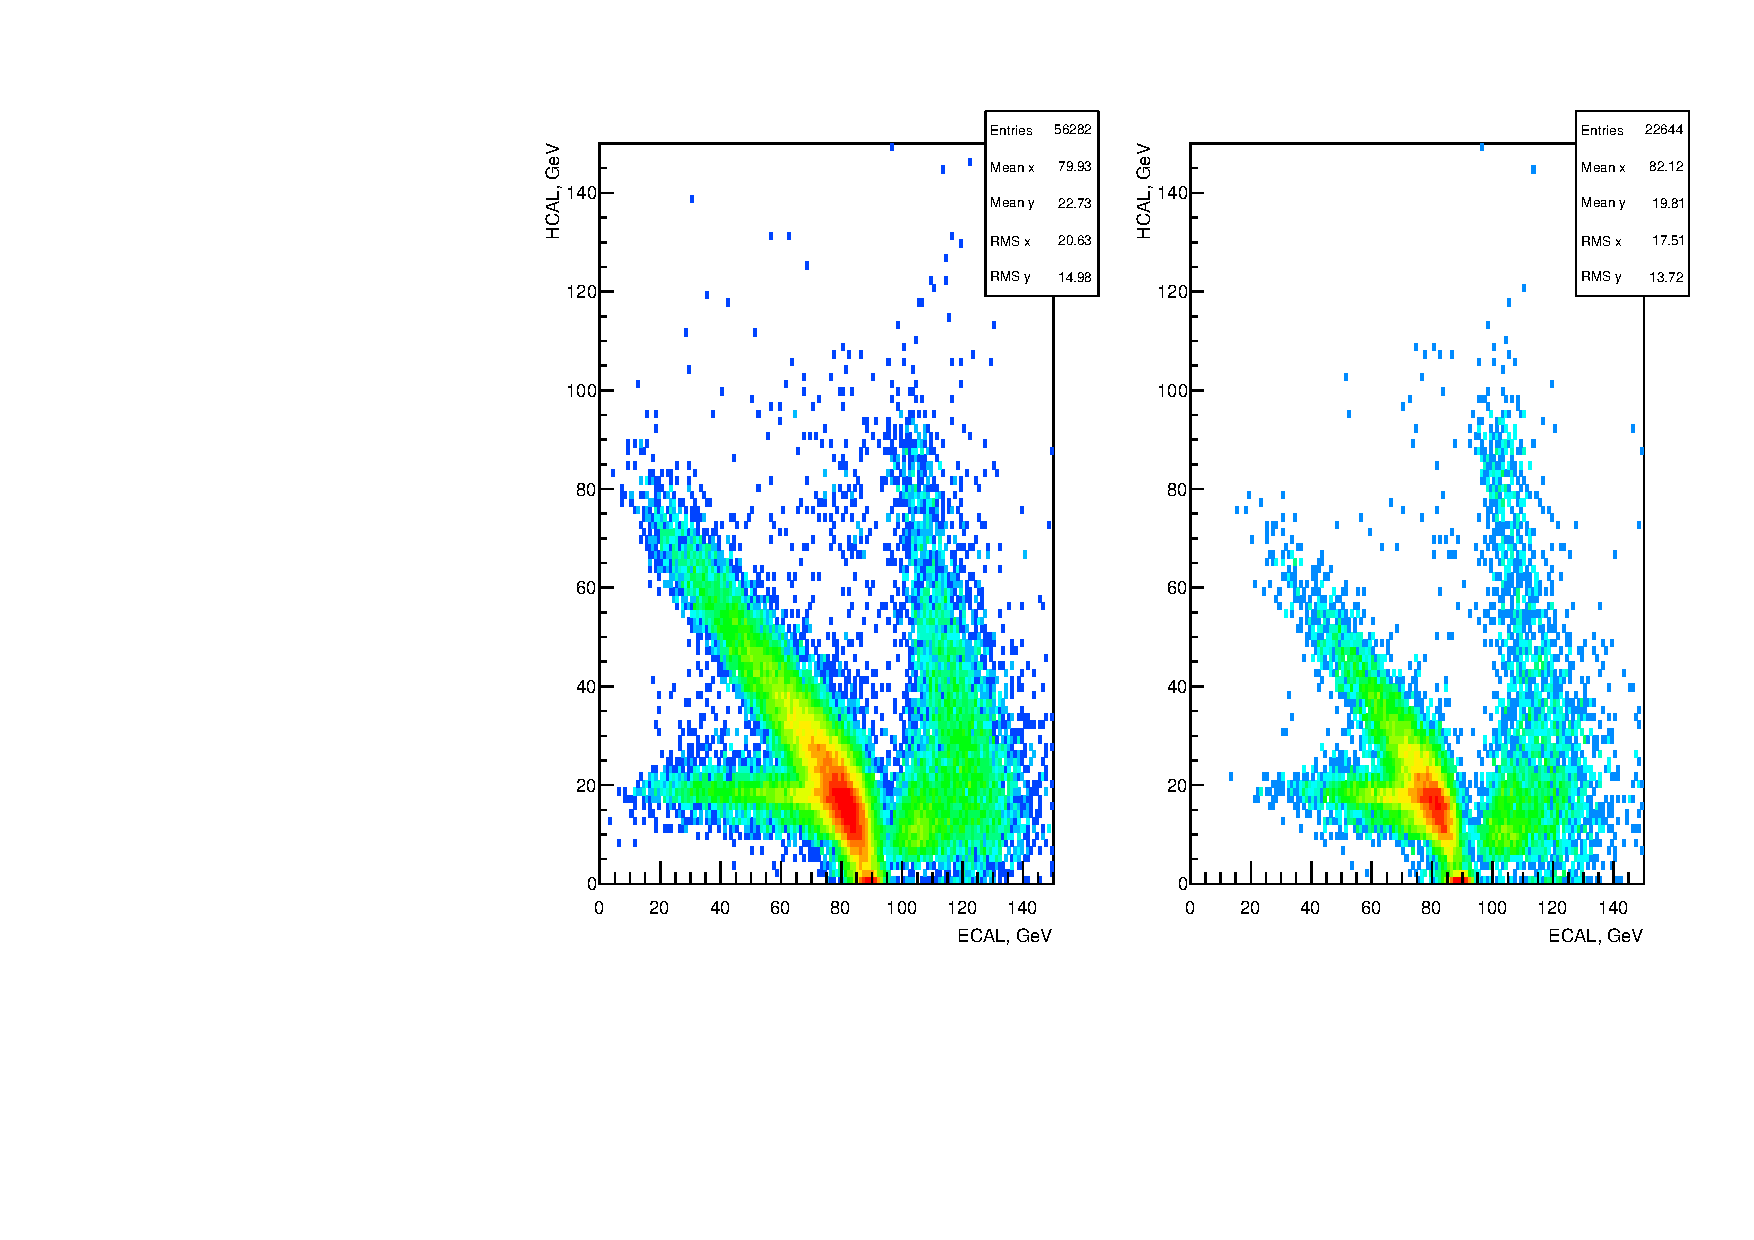
\includegraphics[width=0.95\textwidth,height=0.6\textwidth]{\pdirthree/ehcal_2441_comp.pdf}
  \end{center}
  \caption[ECAL vs HCAL energy deposit after a cut $\chi^2$ for different ECAL configurations]{ECAL vs HCAL after a cut $\chi^2<2$ is applied with the $\chi^2$ calculated with the 9 central cells (left) and for all cells (right).}
  \label{fig:ehcal_comp}
\end{figure}

\iffalse

\section{Comparison with MC}
\label{ch3:sec:mc}
The same profiles described in the section above can be produced using
a 100 GeV electron simulation of the NA64 setup\cite{na64-simulation} and be tested using simulation of $\pi^-$.

We tested qualitatively the effect of a $\chi^{2}$-cut over the
ECAL vs HCAL plots produced for both the MC simulation
and the test runs considered in the previous section. For the
MC-simulation we used the same benchmark cut of the previous section
$\chi^2_{cut}$=2 , while for the data a benchmark cut of
$\chi^2_{cut}$=40 was used to take into account the shift in the
distribution observed.

The bottom plot of Fig.\ref{fig:ehcal_elec} shows that the
contamination of hadron is removed when MC-database is used, so
the hadron shower still produces a significantly larger $\chi^{2}$
compared to the one of an electron shower. The efficiency
observed in the simulation is of ~0.98, slightly larger compared to the data. 
In both simulation and data we can observe that the characteristic
Di-muons events in the range [40,80] GeV in ECAL energy
deposition are accepted.
Fig.\ref{fig:ehcal_hadr} also shows the hadrons to be rejected in both
cases, with a rejection power of $\sim 5\times 10^{-3}$ measured in the
simulation. Also for both simulation and data we can observe that the
events surviving lie mostly in the diagonal $E_{ECAL}$+$E_{HCAL}$= 100
GeV (as could also be observed using a database built from calibration run like in Fig.\ref{fig:ehcal_comp}), while all the events where the shower has large angular spread are rejected.
\\
The main difference between the two plots concerns some events with very low energy deposited in the ECAL that are accepted in the data but not in the simulation. This would suggest that the ECAL cells are subject to some fluctuation that at low energy can sometime mimic the correct electromagnetic-shower signature. As stated in the previous section however for such low energy events the usage of the shower-profile algorithm should be avoided since all the shower will be completely contained in the cell 3x3.\\
% Finally the MC-database was applied to the physical run 2441 always
% with a benchmark cut $\chi^2_{cut}$=40.


\begin{figure}[h!]
  \begin{center}
    \includegraphics[width=0.95\textwidth,height=0.8\textwidth]{\pdirthree/ehcal_2363_chi_mc_2.pdf}
  \end{center}
  \caption{\textbf{Top}: ECAL vs HCAL before (left plot) and
    after (right plot) a cut
    $\chi^2<2$ in MC simulated 100 GeV electron events. \\
    \textbf{Bottom}: ECAL vs HCAL before (left plot) and after (right
    plot) a cut
    $\chi^2<40$ in the electron run 2363.\\
    The $\chi^2$ was computed using all ECAL cells with a shower
    profile database obtained from a 100 GeV $e^-$ MC-simulation. }
  \label{fig:ehcal_elec}
\end{figure}

\begin{figure}[h!]
  \begin{center}
    \includegraphics[width=0.95\textwidth,height=0.8\textwidth]{\pdirthree/ehcal_2204_chi_mc_2.pdf}
  \end{center}
  \caption{\textbf{Top}: ECAL vs HCAL before(left plot) and
    after(right plot) a cut
    $\chi^2<2$ in MC simulated 100 GeV $\pi^-$ events. \\
    \textbf{Bottom}: ECAL vs HCAL before (left plot) and after (right
    plot) a cut
    $\chi^2<40$ in the hadron run 2204.\\
    The $\chi^2$ was computed using all ECAL cells with a shower
    profile database obtained from a 100 GeV $e^-$ MC-simulation. }
  \label{fig:ehcal_hadr}
\end{figure}
\fi

\section{Invisible mode analysis}
\label{ch3:sec:analysis-invis}

The general method of analysis described in Sec.\ref{ch3:sec:analysis-approach} is now applied to the specific case of the invisible mode analysis. To apply the method a set of selection criteria is set to maximize the overall sensitivity of the setup using the MC-simulation described in Sec.\ref{ch3:sec:geant4}. The background is also detailed using the classification defined at the beginning of this chapter. We will show that the expected number of events in the signal region in absence of Dark Photon production is $\simeq 0.5$, making NA64 a background free experiment.

\subsection{Selection criteria}
\label{ch3:sec:selection-criteria}

We define here the selection criteria used in the analysis to maximize our sensitivity. The cuts used are chosen based on their significance in the MC simulation, hence they maximize:

\begin{equation}
  \label{eq:significance}
  S = \frac{s}{\sqrt{s + b}}
\end{equation}

Where $s$ and $b$ are again signal and background. In this context, the signal is not necessarily an event with $\DMM$ production, but the particle that the cut is supposed to select. In the case of SRD for example, the cut is required to select electrons and reject any other kind of particle. So $s$ will be the number of electrons selected by the cut and $b$ will be the number of non-electron ($\pi^-$, $\mu^-$ selected). Since only $e^{-}$ can trigger the reaction $\ea$, this requirement also maximizes the sensitivity of the experiment. The cuts are then optimized using the calibration run and control sample to take into account the effect caused by pileup and electronics as explained in Sec.\ref{ch3:sec:analysis-approach}.

%\subsection{Invisible mode}
%\label{ch3:sec:selection-criteria-invis}

The selection criteria needs to select 100 $\gev$ electrons and reject any events involving interactions before reaching the target. Events are accepted if they surpass the following criteria:

\begin{itemize}
\item The difference between the reconstructed momentum and the nominal beam energy of 100 $\gev$ is not larger than 5 $\gev$. Additionally, the entrance angle of the particle needs to be within 2 $\mrad$ from the mean angle recorded in the calibration run. The track also needs to be reconstructed with a $\chi^2<5$.
\item A deposit of at least 1.3 $\mev$ and not larger than 80 $\mev$ is required in each SRD crystal. Each signal is also required to be in a window of 5 $\nas$. To reject large backscattering from the ECAL, the maximum energy of 120 $\mev$ is allowed in total in the SRD. These cuts ensure the suppression of heavy charged particles in the beam.
\item The energy deposited in the ECAL is required to be in time with $S_0$ within 13 \nas. If more than 30 $\gev$ energy is recorded out of time, the event is rejected. Furthermore, the largest energy deposit in the ECAL needs to be in the ECAL central cell\footnote{The cell is labeled (3$\times$3), a sketch can be seen in Fig.\ref{fig:ecal_example}}. The periphery of the shower is also checked by taking the ratio between the energy deposited outside of the 3$\times$3 matrix that surrounds the central cell and the total energy deposited in the ECAL. Since most of the energy of an em-shower will be deposited inside the Moliere radius, the value outside of it should be below 5\% of the total energy deposited. Finally, the compatibility with an em-shower is checked using the method described in Sec.\ref{ch3:sec:bkg-ecal-profile} with a cut $\chi^2 < 8$.
\item All events with signal above noise in the VETO are rejected to avoid punch-through from the main target. The precise value of the cut is defined as 0.9$\times \emip$.
\item Events where the energy deposited in one of the cells in the periphery of the HCAL is larger than the one deposited in the center are rejected.
\item Events with multiple hits in the straw chamber are removed from the analysis. This cut is used to remove the contamination due to electron-hadron production upstream of the ECAL.
\end{itemize}

Finally, the signal region is defined by events with significant missing energy in the ECAL and no activity in the HCAL. This means $E_{ECAL} < 50$ $\gev$ and $E_{HCAL} < 1$ $\gev$, previously illustrated in Fig.\ref{fig:two-signature}.

The efficiency of the cuts listed above was studied using the MC simulation and the electron calibration runs.
%A small summary of the uncertainty is provided in Table \ref{tab:inv-cut-eff}.
The effect of these cuts can be appreciated in the $\ehcalplane$ plane, where the evolution from the original sample is particularly relevant. These effects are shown in Fig.\ref{fig:inv-cut-ehcal}, most notably the amount of hadrons is seen to greatly reduced after the SRD cut is applied, and consequentially the dimuon region becomes more visible. The VETO cut then removes most of the punchthrough particles, including dimuons. Finally, when the tracking selection criteria are applied, a large portion of the low energy deposit event and strong scattering upstream disappear\footnote{This is mostly visible in the requirement of "GoodTrack", visible between plot 5 and 6}.


\begin{figure}[bth!]
  \centering
   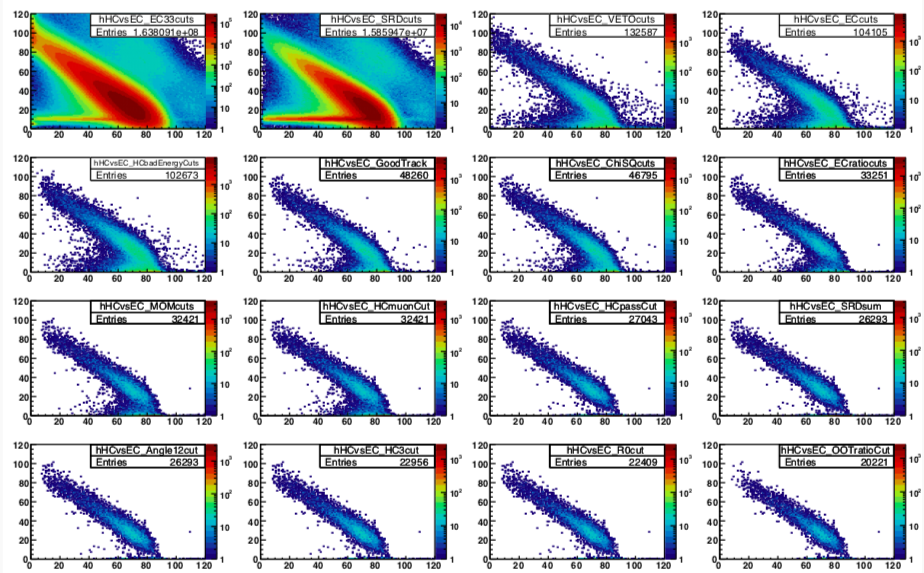
\includegraphics[width=\textwidth]{\pdirthree/ec-hc-plots-veto-nobad-runs.png}
  %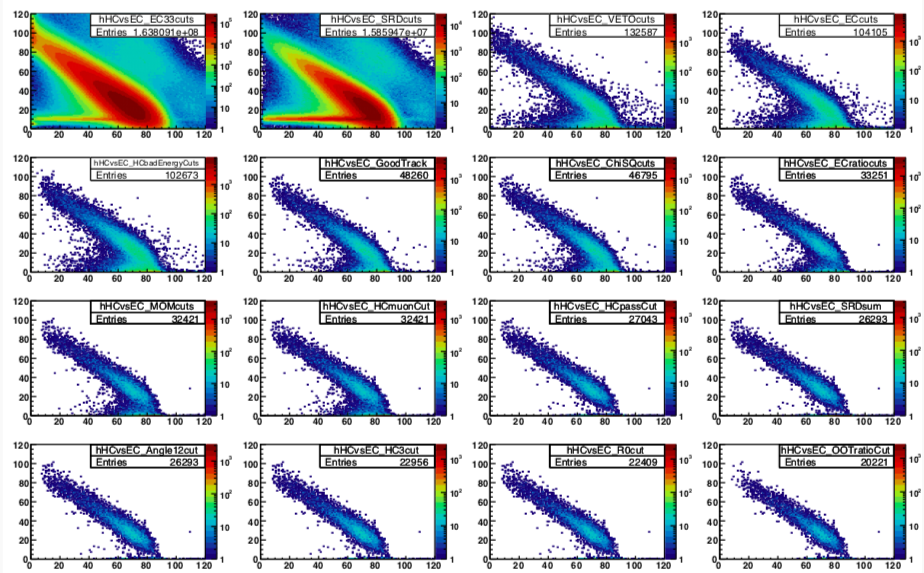
\includegraphics[width=\textwidth]{\pdirthree/ec-hc-plots-veto-nobad-runs.pdf}
  \caption[effect of the cuts in invisible mode]{Effect of selection criteria in the $\ehcalplane$ on the sample of data collected in 2018 invisible mode \cite{invis-cut-plot,NA64:2019imj}.}
  \label{fig:inv-cut-ehcal}
\end{figure}

\subsection{Background}
\label{ch3:sec:bkg:inv}

In this section, we will try to go more in detail of what constitutes background in invisible mode setup, following the classification defined in Sec.\ref{ch3:sec:analysis-approach}. A complete summary of the expected background, including uncertainty for each single source, is provided in Table \ref{tab:inv-bkg}.
\subsubsection{Hadronic background}
\label{ch3:sec:bkg:inv:hadr}


In the case of invisible mode, the \textbf{Hadronic background} can arise simply from a $\pi^-$ that after leaving minimal energy in the ECAL, travels through the HCAL undetected. The probability of this happening with a total interaction length of 21 $\lambda_{int}$ is $p\lesssim 10^{-9}$. This number does not account for the high-efficiency VETO after the ECAL, SRD rejection, and the fact that the HCAL can detect a MIP interaction even without an inelastic interaction happening. Each of these factors pushes the background well below $<10^{-13}$ as pointed out in the NA64 first proposal \cite{Andreas:2013lya}. A more relevant background would be an inelastic scattering inside the ECAL in a process:

\begin{equation}
  \label{eq:pion-nucleus-scattering}
  h + Z \longrightarrow h + Z + (hadrons)
\end{equation}

In this process, part of the energy can evaporate as a consequence of some particles emitted at a large angle and thus escaping the setup in the direction transverse to the beam. This background is suppressed by shower profile analysis, energy deposited in the pre-shower, and the VETO cut. The phase space of this process is however very complicate, and a lot of possible phenomenologies can arise from it. For example, large energy deposited in the pre-shower can be a simple consequence of some $\pi^0$ backscattering after the hadronization, while the shower profile can mimic the one of an electron if a large fraction of energy in the inelastic scattering is carried away by $\pi^0$. Also, if particles are emitted in the form of neutrons or other neutrals as $\ks$, the VETO would be ineffective to reject them.

To have an estimate, we can take the process \ref{eq:pion-nucleus-scattering} and assume $\geq$2 neutrals particles are produced in the hadronization. This gives us a probability equal to \cite{gkkk1}:

\begin{equation}
  \label{eq:transverse-leak-estimate}
  P \simeq P_n \cdot P_{la} \cdot P_{leak}
\end{equation}

Where we define $P_n$ the probability of such interaction to occur, $P_{la}$ the probability to produce particles at large scattering angle, and $P_{leak}$ the probability to escape HCAL without interactions. Here we stress again that this formula hides a large number of topologies that such an event could have, but is instructive to get an intuition for these processes. Since the ECAL has $\lambda_{int} \simeq 0.5$, the probability of interaction for an hadron is fairly high (roughly 50\% of the time such interaction will happen). We need at least 50 $\gev$ of energy leaking to produce a signal event. If we assume two neutrals to be produced at $\Theta_{n} \simeq 30$\si{\degree} this would mean crossing at least 4$\lambda_{int}$ each, for a $P_{leak} \lesssim 3 \cdot 10^{-4}$. We can take the measured values of NOMAD to estimate the value of the cross-section in this range \cite{AUTIERO1998285,GNINENKO1998583}. The probability of separating a cluster with energy $>$0.1E$_{\pi}$ at an angle $\Theta_{n} \gtrsim 30$\si{\degree} was measured to be P$_{la} \simeq 10^{-5}$ and it drops very quickly with the beam energy: a factor 20 difference was found between 15 $\gev$ and 6 $\gev$ $\pi^-$. Even if we take conservative value as $P_{la}$, we see that the probability of the energy to escape is already $P\simeq 10^{-9}$, which multiplied to the hadron contamination and SRD suppression leads to an estimate of $P<10^{-14}$ for this background.

Another possible background is the decay of hadron inside the setup in neutrinos, which would cause some energy to disappear from the setup. The high energy of the primary suppress this background, since at 100 GeV the chance for a $\pi^-/K^-$ to decay is $P^{decay}_{\pi} \simeq  10^{-2}$(\footnote{calculated for a total length of 20 m assuming light-speed.}). Multiple possible decays are accompanied by a neutrino emission, the most likely one being the $\pi^-$ decay $\pi^- \rightarrow mu^- \nu_{\mu}$. The emission of the muon makes such decay very easy to spot, since it will leave an energy deposit both in the VETO and the HCAL, for a total probability similar to the one of a punch-through $\pi^-$ ($P < 10^{-14}$). One could argue that the $\mu^-$ could decay: $\mu^- \rightarrow e^- + \nu_{mu}+ \hbar{\nu_{e}}$, producing an electromagnetic shower with missing energy. The long decay time of the $\mu^-$ adds however an additional suppression factor of $P\simeq 10^{-5}$, which together with the upstream selection criteria put the background conservatively at $P \lesssim 10^{-13}$.

Another background comes from a decay of $K^-$: $K^- \rightarrow \pi^0 + e^- + \hbar{\nu_e}$, commonly called $K^-_{3e}$, with a branching ratio of $\Gamma_i/\Gamma_{tot} \approx$0.05 \cite{particle-strange-mesons}. The total probability of background for an incoming $K^-$ is around $P\simeq 10^{-3}$ accounting for both probabilities of decay and branching ratio. A MC-simulation of $K^-$ confirms this simple estimate as shown in Fig.\ref{fig:kaonbkg-sim}, where the fraction of the events in the signal region corresponds to the probability calculated. Multiplying this probability for the SRD selection criteria and the suppression from the beam returns a probability of $P_{K_{3e}} < 10^{-12}$. %\footnote{Here a suppression from the beam of 10$^{-3}$ is used, since the $K^-$ is a smaller fraction than the contamination \cite{h4-beamline}}.
There are however additional factors of rejection for this background that can be investigated using MC-simulations. A more precise account of SRD in this scenario and the effects of the tracking and shower profile push this background to $P_{K_{3e}} \lesssim 10^{-13}$.


\begin{figure}[bth!]
  \centering
  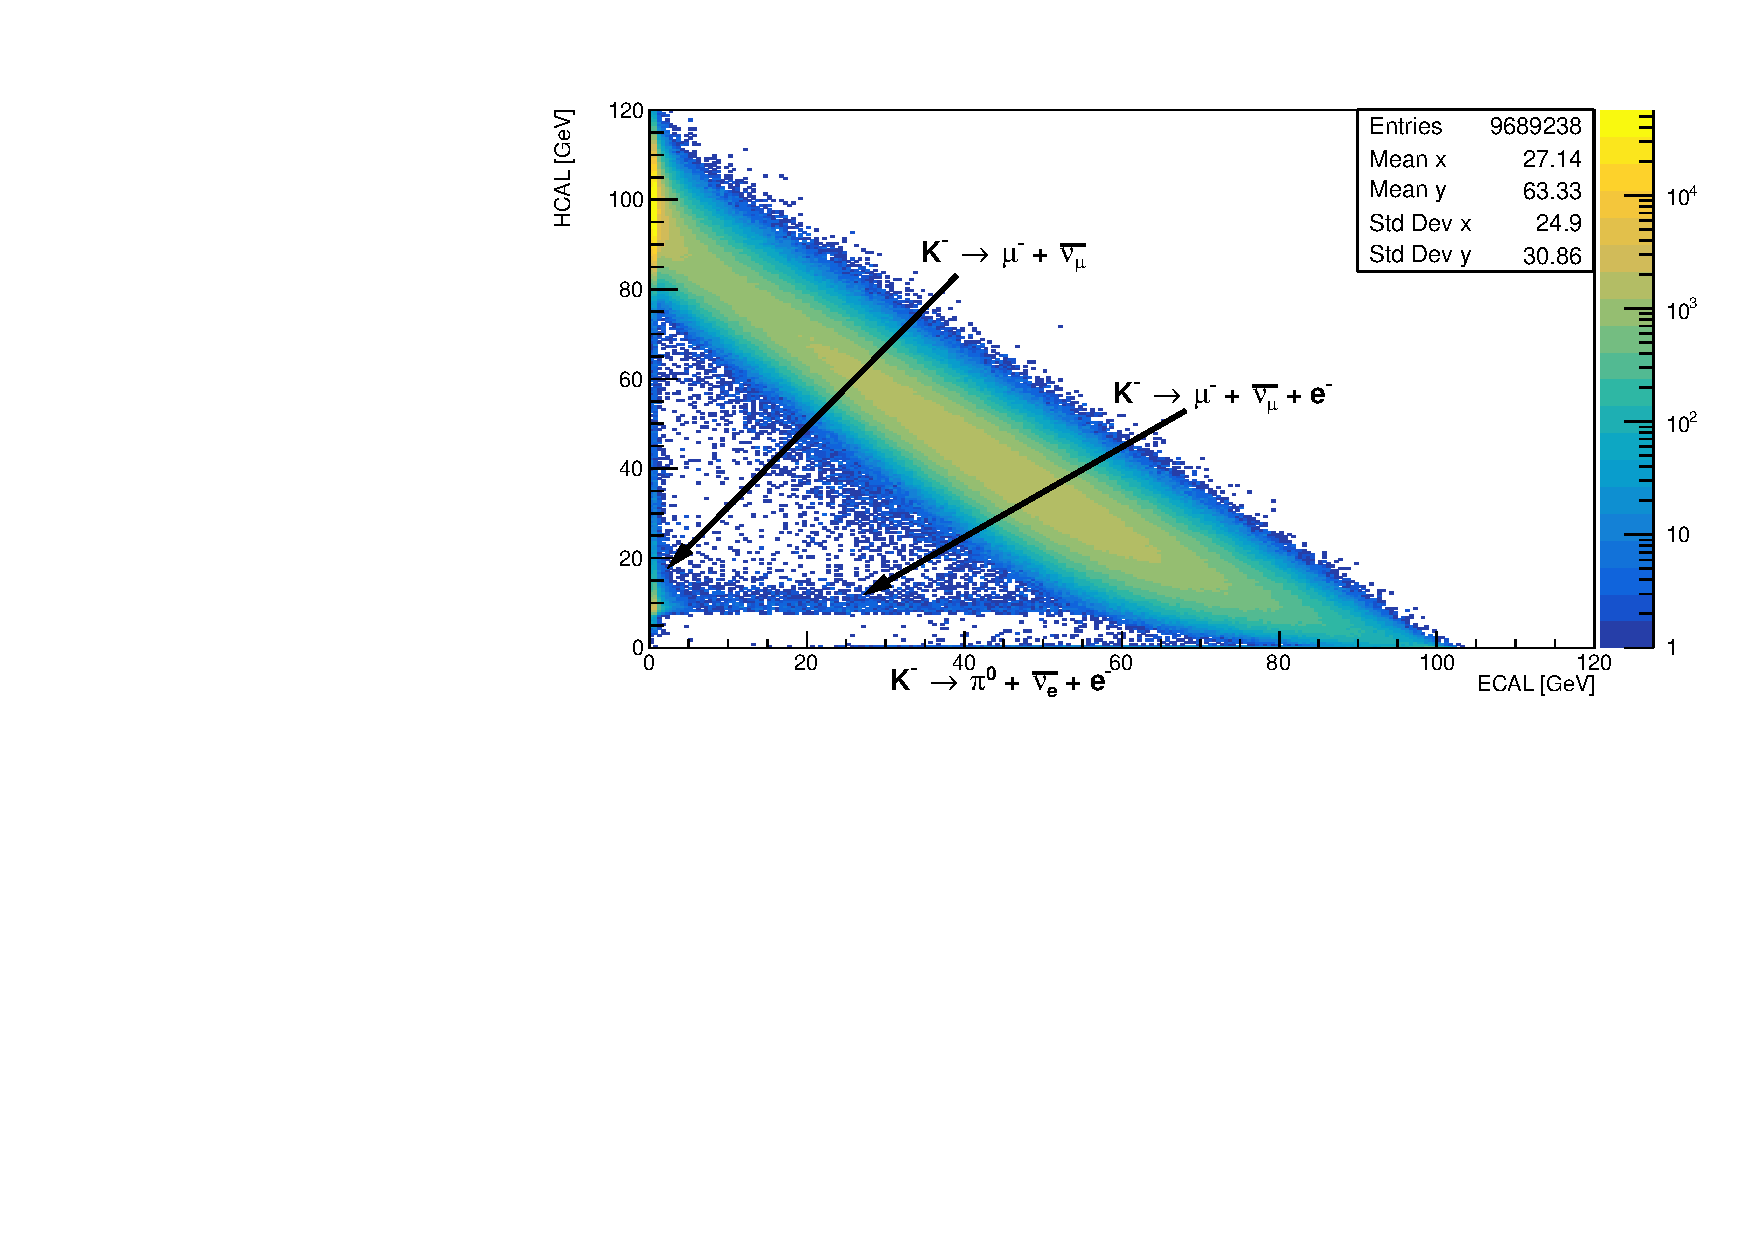
\includegraphics[width=\textwidth]{\pdirthree/kaonbkg.pdf}
  \caption[$K^-$ simulation ]{Energy deposited in the $\ehcalplane$ plane after simulating $10^7$ $K^-$ as primary particle in the NA64 setup.}
  \label{fig:kaonbkg-sim}
\end{figure}

\subsubsection{Muonic background}
\label{ch3:sec:bkg:inv:muon}

This type of background is also largely suppressed by both beam composition and SRD selection criteria, to a level of
%\footnote{Here the suppression from the beam composition is larger ($10^{-3}$) \cite{h4-beamline} and SRD selection criteria are more stringent ($10^{-4}$) due to the absence of back-scattering.}
$\lesssim 10^{-7}$. As in the case of $\pi^-$, we can convince ourselves that a complete punch-through of the setup without being detected is negligible. Indeed the muon needs to travel through both the VETO and 3 HCAL modules without leaving any detectable energy deposit. Using $p^{VETO} \simeq 10^{-3}$ for leaving undetectable energy in the VETO and $p^{HCAL} \simeq 10^{-4}$ to deposit less energy than the threshold in all modules, we see that the background is conservatively $< 10^{-14}$. In the case of muons, nuclear interaction is less likely. Thus, there is no chance for a large amount of energy to escape transversely. What remains is the decay $\mu^- \rightarrow e\nu\nu$, with neutrinos in the final state. The decay time of $\mu^-$ adds a suppression of $\lesssim 10^{-5}$. Similar to the previous case, proper accounting of SRD, tracking, and shower profile accounts for an additional $p\sim 0.1$ factor. The final level of this background is of $P_{\mu} \lesssim 10^{-13}$.

\subsubsection{Electronic background}
\label{ch3:sec:bkg:inv:elec}

The last type of background is originating from electron primary. Since the beam is primarily made of electrons, and SRD are tuned to select them, no upstream suppression factor can be achieved. Simple punch-through of an electron through the whole setup is not possible, since the path is blocked by 3 HCAL modules. Other similar events, with energy losses due to non-uniformity and cracks in the ECAL/HCAL were as well studied and found unrealistic \cite{Andreas:2013lya}. Low energy electrons is also potentially background: if a primary electron with $E_0 < E_{th}$ arrives at the ECAL it will leave an energy deposit compatible with the signal. Such a background was also found extremely unlikely. The amount of electron $N(E_e<E_{th})$ in the beam with energy lower than the energy threshold for the signal amounts conservatively to $<10^{-2}$. Such particles are normally deflected by the two MBPL magnets outside the acceptance of the ECAL\footnote{A quick calculation shows that for $E_0$=50 $\gev$ the difference in deviation is about 0.4 \si{\meter}}. The tracking system in NA64 makes sure that the energy of the incoming particle is always measured with a resolution of $\delta p/p \approx 1\%$ \cite{Banerjee:2017mdu}, particles with large entrance angle in the magnet can in principle enter in the acceptance of the magnet, but their momentum is reconstructed by observing their displacement in the Micromegas. A dedicated simulation of $10^{10}$ EOT was performed by simulating electrons with energy compatible with the signal region. No event was found in the signal region after requiring a reconstructed momentum within 3$\sigma$. This allows us to put this background conservatively at a level of $\lesssim 10^{-13}$.

An important source of background to be considered is the dimuon production inside the target. As mentioned, these events are very useful to check for systematics and validated the MC. However, fluctuation in the energy deposited in the HCAL might leak in the signal region. The background was estimated by exponential extrapolation of the control sample inside the signal region ($E_{HCAL} < 1 \gev$) considering the sideband I depicted in Fig.\ref{fig:ehcal-bkg-bands}. This estimate was performed using the control sample without applying the VETO cut, that is then taken into account as a factor $\sim 10^{-6}$ (probability of two MIP to leave no energy).

\begin{figure}[bth!]
  \centering
  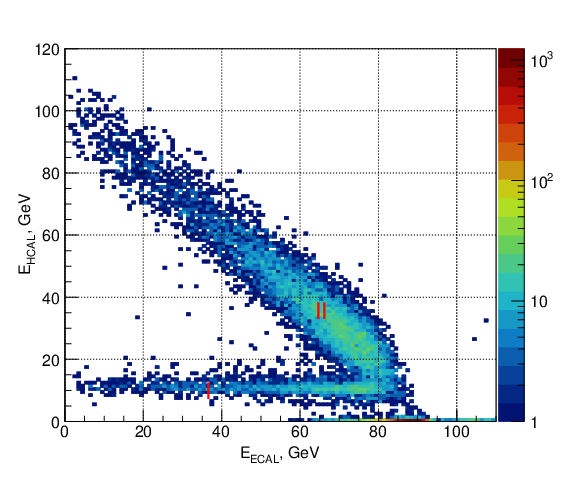
\includegraphics[width=0.45\textwidth]{\pdirthree/EHCAL_lastpub_left.png}
  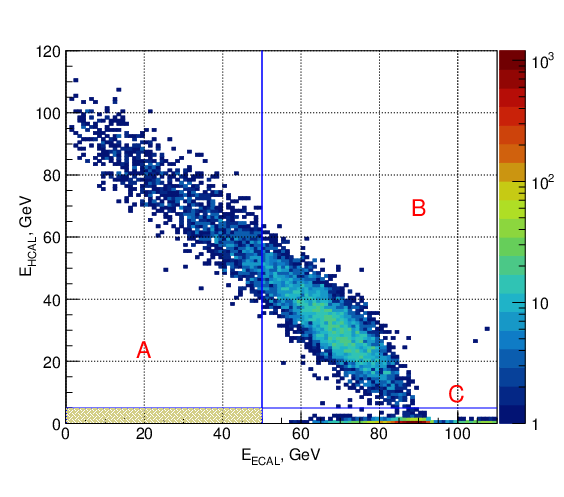
\includegraphics[width=0.45\textwidth]{\pdirthree/EHCAL_lastpub_right.png}
  \caption[ECAL vs HCAL events band]{Distribution of events in the $\ehcalplane$ plane for the control sample of the data. The right panel shows the sample with all the selection criteria. The left panel shows the same sample without the VETO cut. The shaded area is the signal box. The size of the signal box is increased by a factor 5 in the Y-axis direction for illustration purposes. The region labeled I contains events caused by dimuon production, while region II contains mostly event leaking from the ECAL into the HCAL. The sidebands A and C are used to estimate the background inside the signal region \cite{NA64:2019imj}.}
  \label{fig:ehcal-bkg-bands}
\end{figure}

Finally, the leading background in the invisible mode setup is the electro-nuclear and photo-nuclear production of neutral hadrons at a large angle. This case is similar to the one discussed for hadrons, but no additional suppression due to beam-composition and SRD selection criteria is present. In first approximation, the rarity of such interaction balances the absence of suppression factors, and accounts for $P_n \simeq 10^{-6}$ (see Eq.\ref{eq:transverse-leak-estimate}).
The largest source of background, however, comes from electro-nuclear production happening upstream of the target. As Fig.\ref{fig:eh-prod-sketch} shows, if this interaction happens in a detector with a large distance from the ECAL, the displacement of the particle can be large enough to exit the setup transversely. 


\begin{figure}[bth!]
  \centering
  \includegraphics[scale=0.4]{\pdirthree/hcal-leak.pdf}
  \caption[upstream electro-hadron production upstream]{Sketch of electro-nuclear interaction happening upstream the ECAL leading to a possible background \cite{pdegen-thesis}.}
  \label{fig:eh-prod-sketch}
\end{figure}

This background can be estimated by looking at the periphery region of the HCAL. Since the angular distribution is sharply suppressed for large angle \cite{AUTIERO1998285,GNINENKO1998583}, these particles typically leave an energy signature in the periphery of the first HCAL when they miss the ECAL. For this purpose, we define the variable R, defined as the ratio between energy deposited in all cell excluded the central one, and the total energy deposited in the modules:

\begin{equation}
  \label{eq:R-factor}
  R = \frac{E^{all}_{HCAL} - E^{center}_{HCAL}}{ECAL^{all}_{HCAL}}
\end{equation}

In a normal event with particles leaking the ECAL, we typically observe $R<0.5$, as the HCAL module center is aligned with the beam direction, thus the dominating energy deposit will be in the central cell. If an electro-nuclear production happens upstream however, some distortion of this variable will be visible. In the most extreme scenario when the particle is missing the ECAL completely, the R value can be equal 1, since the central cell of the HCAL will be shielded by the ECAL while the periphery will be directly hit. We can observe such behavior in Fig.\ref{fig:r-value-csample}: most of the event considered have an R peaked at 0.35. Events, where the primary electron loses a large portion of its energy due to bremsstrahlung, are shown in region III and are responsible for events with large R. In this topology of events, the electron completely misses the ECAL after being deflected by the magnetic field, while the hard-$\gamma$ produced in the interaction propagates without being deflected and hits the HCAL in the periphery. Such events are also easily identifiable by looking at the HCAL placed in from the original beam direction. In the event of region III, this detector measure energy deposit $E>60$ $\gev$.

\begin{figure}[bth!]
  \centering
  \includegraphics[width=\textwidth]{\pdirthree/pp30-calsr-uncut-may2.pdf}
  \caption[R value for control sample]{Energy distribution in the $\ehcalplane$ (left) and the corresponding distribution of the R for different interesting regions. Region I is populated by the dimuon production inside the ECAL. Region II are events leaking in the HCAL characterized by energy conservation. Region III contains events with hard bremsstrahlung of the $e^-$ upstream, where the primary completely miss the ECAL and the $\gamma$ energy is deposited in the HCAL periphery. Region IV is characterized by pileup events \cite{pdegen-thesis}.}
  \label{fig:r-value-csample}
\end{figure}

Events with electro-nuclear scattering upstream are characterized by a distribution equivalent to the one of region III. The agreement of the R distribution between data and simulation was checked using data of HCAL and ECAL calibration runs, which shows a good fit with the simulated samples and small differences between different species of hadrons. This background can be suppressed by two additional tools:

\begin{itemize}
\item The straw tube in the beamline, as shown in Fig.\ref{fig:eh-prod-sketch} are in the way of the hadrons and can detect them in the periphery of their active area. A simple constraint that requires all hit to be within 3$\sigma_{beam}$ can reject this background effectively. A cut based on the multiplicity of the hit was observed to be equally powerful, since electro-nuclear interaction will produce a large number of particles in the final state. \cite{pdegen-thesis}.
\item Since electronuclear interactions produce a large number of particles, this interaction saturates the MM detector strip output. A cut based on the total charge deposited in each plane is also effective to suppress the background \cite{na64-invisible-cuts}.
\end{itemize}

The first cut removed the contamination in the control sample, and where accounted for in the final background estimate. In practice, the background was extrapolated using an exponential distribution of the type:

\begin{equation}
  \label{eq:bkg-extrapolation}
  e^{a \cdot E_{ECAL} + b}
\end{equation}

The parameters $a$ and $b$ are fitted using the data in the sideband C of the control sample, i.e. events with E$_{HCAL}<$ 1 $\gev$ and $E_{ECAL}>E_{th}$, and then integrated over the signal region. The results of this estimate were then accounted for conservatively in Table \ref{tab:inv-bkg}.

\begin{figure}[bht!]
  \centering
  \includegraphics[width=\textwidth]{\pdirthree/HCraio-e-428-pi-3924-MC.pdf}
  \caption[R value comparison]{Distribution of the R variable for the 80 $\gev$ $e^-$, $\pi^-$, $K_L^0$ and n events obtained from data during the ECAL and HCAL calibration runs \cite{Banerjee:2020fue}.}
  \label{fig:R-comp}
\end{figure}

\begin{table}[bth!]
  \centering
  \caption[Invisible mode background]{Expected background for 2.84 $\times$ $10^{11}$ EOT collected at the time this thesis was written \cite{NA64:2019imj}}
  \begin{tabular}{lr}
    \hline \hline
    Background source & Background, $n_b$ \\
    \hline
    $\pi^-$,$\mu^-$ punchthrough                      & $<10^{-14}$ \\
    low energy $e^-$                                  & $<10^{-13}$ \\
    $e^-$/hadron nuclear interaction in target        & $<0.044$   \\
    $\pi^-$,$\mu^-$, $K_{3e}$ decay                    & 0.02 $\pm$ 0.01 \\
    $e^-$ nuclear interaction in the  beam line       & 0.43 $\pm$ 0.16 \\
    \hline
    Total (conservatively)                            & 0.53 $\pm$ 0.17 \\
    \hline \hline                       
  \end{tabular}
  \label{tab:inv-bkg}
\end{table}



\section{Visible mode analysis}
\label{ch3:sec:analysis-vis}

In this section, we provide the selection criteria and background condition specific to the visible mode search. A new analysis I performed using the 4 GEMs tracker inside the decay volume is also described here. The validation of the MC and signal correction is also performed following the method described in Sec.\ref{ch3:sec:dimuons}, but also including a new tracking procedure developed to reconstruct vertex candidates in the decay volume. The background condition is similar for this analysis, as the selection criteria only differ for the low energy $\DMM$ produced in the late stage of the em-shower.

\subsection{Selection criteria}
\label{ch3:sec:selection-criteria-vis}

For the visible mode, the signal is searched by matching the energy deposited in the target with the one detected by the ECAL downstream. Similarly to the invisible mode, several selection criteria ensure that the incoming particle is a well-defined electron track. Although the tracking procedure is still used to work with the control sample, the incoming particle is not required to have a momentum matching the nominal beam energy. This is because the energy conservation selection criteria already ensure that the particle will have a well-defined energy. The selection criteria for the visible mode can be summarized as follow:

\begin{itemize}
\item An energy above 1 $\mev$ is required in each SRD, and the total energy detected in both counters needs to be larger than 10 $\mev$. Events, where the energy deposit surpasses 200 $\mev$, are removed to suppress large scattering upstream or backscattering from the WCAL.
\item Energy deposit $E_{PS} > 5 \gev$ compatible with an electron in the WCAL pre-shower.
\item Energy deposited in S4 compatible with two MIP in the decay volume. This cut amounts to $E_{S_4} > $1.5$\times \emip$.
\item At least 25 $\gev$ deposited in the ECAL. This cut rejects events where low energy particle punch-through the WCAL.
\item The maximal energy of the shower should be deposited in the cell of the ECAL aligned with the beam axis (labeled as 3$\times$3). The longitudinal and lateral shape of the shower should be consistent with a single em-shower\footnote{Although the signal is expected from a $\ee$ pair, the distance of just a few $\mmi$ between the two particles does not allow for a separation between the two showers}. This means a maximal energy of 3 $\gev$ is allowed in the pre-shower of the ECAL and a compatibility of the transversal shape $\chi^2 < 10$ is required.
\item  No energy deposit in the W2 counter placed after the WCAL. The value of this cut is $E_{W2} < $0.7$\times \emip$ \cite{Banerjee:2019hmi}.  
\item Energy deposited in the VETO has to be smaller than 0.9$\times \emip$, energy deposited in each HCAL modules needs to be smaller than 1 $\gev$.  
\end{itemize}

The signal region is finally defined by looking at events where the sum of WCAL and ECAL energy is matching the nominal beam energy within the energy resolution of the detectors (see Fig.\ref{fig:two-signature}). This energy was originally 100 $\gev$ in 2017, but was increased to 150 $\gev$ in 2018 to boost the sensitivity for short-lived $\DMX$ (see Fig.\ref{fig:w-e-vis}).

\subsection{Visible mode analysis using the tracking approach}
\label{ch3:sec:vis-mode-tracking}

The published analysis using the data collected in 2018 \cite{Banerjee:2019hmi} was based exclusively on the calorimeters and counters as described in Sec.\ref{ch2:sec:vismode}. The trackers after the decay volume were not used for signal discrimination. Here we present a novel method that exploits them providing a boost in the signal yields while maintaining the background under control. Even though this analysis is not sensitive when the decay length of the $\DMM$ is significantly smaller than the dimension of the dump, it has the advantage of being complementary to the calorimeter analysis. Unfortunately, the particularly interesting parameter space justifying the protophobic vector boson explanation of the $^8$Be anomaly is not significantly ($\lesssim$1\%) improved by this approach, the reason being the small decay length of $\DMX$ in the high-coupling region. It provides however an independent confirmation of the results obtained in \cite{Banerjee:2019hmi}, and a confirmation of the tracking procedure that be used in the next generation of this experiment (see Sec.\ref{ch5:sec:new-vismode-setup}).

While in a first approximation the $\DMM$ is produced in the first few layers of the WCAL, it can also originate at a later stage of the em-shower. These events, which are typically rejected in the calorimeter analysis, are instead accepted in the new analysis presented here. First, an initial sample is selected in the same way described above. The final discrimination in the calorimeter analysis is based on the counter W2 placed at the end of the dump to reject the charged punch-through from the em-shower. This last cut is efficient if the $\DMM$ is produced in the first few layers of the WCAL but typically rejects the event if the $\DMM$ is produced at a later stage of the em-shower. The reason is that these events are accompanied by a long longitudinal development of the em-shower that leaves an energy deposit larger than the typical energy cut accepted in the calorimeter analysis. On the other hand, the low energy of the produced $\DMM$ implies a larger angle between the decay products that can be resolved by the trackers. Combining these two concepts, one can see that the signal yield is characterized by two different topologies that can be easily distinguished by looking at the energy deposited in the ECAL (see Fig.\ref{fig:combined-analysis}).

Using this distinction, we divide all events that passed the initial selection criteria in two topologies based on the total energy deposited in the ECAL. The exact value of this threshold was selected to maximize the signal yield. The optimal value has a small dependence on the $\DMM$ mass and coupling. A simple threshold of 75 GeV amounting to half of the initial beam energy was found to be robust for most of the interesting signal scenario. After the topology is decided, a final set of cuts is applied to discriminate between signal and background. In the case of high energy $\DMM$, trackers do not have the capability of discriminating between single hits. If the energy deposited in the ECAL surpasses the 75 $\gev$, the selection criteria applied will be the one one described in the previous section. On the other hand, if the energy deposited in the ECAL is smaller than 75 GeV, trackers are used instead of the W2 as discriminator for an $\DMM$ production. Two tracks in the decay volume are required with a reconstructed vertex within 3$\sigma$ from the WCAL and an angle smaller than 3 $\mrad$. This different treatment leads to increased efficiency of the $\DMM$ produced at a late stage of the shower as shown in Fig.\ref{fig:combined-analysis}. However, the smaller energy of the $\DMM$ produced in this way has the effect of reducing the probability of the particle escaping the dump. For large coupling $\epsilon$ this suppression can be more than 2 orders of magnitude, making the boost of signal yield negligible. A summary of this boost for various interesting $\DMM$ scenario is illustrated in Table \ref{tab:dm:efftable}. The values reported consider also a conservative correction factor of 0.77$\pm$0.1 that takes into account inefficiencies of the detectors and the reconstruction algorithm. This factor was evaluated using a data-driven method precisely outlined in Sec.\ref{ch3:sec:dimuons}. We conclude that in the current setup trackers do not improve the limit on the $\DMX$ parameter space significantly. This is because the boost in signal yield becomes negligible for $\epsilon \sim 6 \times 10^{-4}$, a value which is already excluded with 90\% confidence by our previous analysis \cite{Banerjee:2019hmi}.

\begin{figure}[tbh!]
  \centering
  \includegraphics[width=\textwidth]{\pdirthree/X17-separation-v2.png}
  \caption[Comparison of selected $\DM$ between the calorimeter and tracking analysis]{$\DM$ simulated in the visible mode 2018 setup. Two different cuts are used to discriminate between two $\DM$ topologies. The first one is based on angle cut and vertex position using information from the 4 GEM stations installed in the decay volume and is very efficient on the $\DM$ produced at low energy (red triangle). The second one relies on the Veto placed at the end of the dump and is more efficient for the high energy population (blue square).}
  \label{fig:combined-analysis}
\end{figure}

\begin{table}[h!]
  \centering
  \begin{tabular}{|llr|}
    \hline
    M$_{A'}$ [MeV]& $\epsilon$ & N$^{new}_{A'}$ / N$^{old}_{A'}$ \\    
    \hline
    5    & 0.004    & 1   \\    
    1    & 0.0015   & 1   \\    
    1    & 0.003    & 1   \\    
    16.7 & 0.0001   & 1.22\\
    16.7 & 0.00018  & 1.2 \\    
    16.7 & 0.000316 & 1.2 \\
    16.7 & 0.0006   & 1.01\\
    16.7 & 0.0007   & 1   \\
    22   & 0.000316 & 1.22\\
    \hline    
  \end{tabular}
  \caption[ratio between signal events observed in tracker-analysis compared to calorimeter-only analysis]{N$^{new}_{A'}$ / N$^{old}_{A'}$ ratio between signal events observed in tracker-analysis compared to calorimeter-only analysis. The new analysis uses cuts based on GEM tracking detectors if the energy detected by the downstream ECAL is below 75 GeV.}
  \label{tab:dm:efftable}
\end{table}

\subsubsection{$\gamma + Z \rightarrow \mu^+ \mu^-$ events in the visible mode analysis using trackers}
\label{ch3:sec:vis-mode-tracking-dimuon}

To validate the MC simulation and the tracking procedure required for this analysis, a pure sample of events containing the rare QED interaction $\emu$ has been studied. The double tracks expected in the decay volume are then used to test the reliability of the tracking procedure in the setup. In the MC, the tracks are prepared following the procedure describe in Sec.\ref{ch3:sec:geant4-digitization} to transform the pure hits received by the MC in a common hit class that reproduces the behaviour of the GEMs detector. These tracks are then fed to the same reconstruction algorithm used for the data.

The reconstruction chain works as follows:
\begin{enumerate}
\item Track candidates are defined by grouping hits where the angle between first and second GEM pair is smaller than 9 mrad.
\item Those candidates are reconstructed using a Kalman filter implemented with the Genfit library \cite{genfit}.
\item Vertex candidates are generated by grouping tracks pair with no common hits.
\item The exact position of the vertex is obtained by back-propagating the tracks at their point of minimum distance. Only vertices with a distance below 3 $\mmi$ are considered for the analysis.
\end{enumerate}

\begin{figure}[tbh!]
  \begin{center}
    \includegraphics[scale=0.8]{\pdirthree/GEM4_rel.pdf}
  \end{center}

  \caption[Hit position of $\emu$ in GEM MC-DATA]{Hit position recorded in last GEM before ECAL for MC simulated (Red curve) and data (Blue dots) $\emu$ events.}
  \label{fig:dimuon:gemspectra}
\end{figure}
  

A dimuon sample was selected using all events collected during the visible mode 2018 run. The beam quality was improved by requiring a reconstructed momentum in the range between 140 and 160 GeV. The $\emu$ events leave a double-MIP signature in each HCAL module, thus a cut 2 GeV$<$ E$_{hcal} <$ 6.35 GeV is applied for the selection. Since the physical trigger is used during the data taking (see Sec.\ref{ch2:sec:detectors-trigger}), an additional cut $E_{WCAL} < 90$ GeV is applied to consider only such events in both simulation and data. This cut also selects a sample with kinematics closer to the one expected from a $\DM$ candidate. This makes the comparison with the MC more significant for our search. Scintillator counters also need to be compatible with a $\mu^+ \mu^-$ in the decay volume: an energy deposited of at least 1 MIP is required in the scintillator (S4) downstream the WCAL and at least 1.8 MIP in the Veto behind the ECAL. The less stringent cut on S4 is justified by its limited transverse dimension which makes it not suitable for a precise energy measurement.

Although these cuts mainly select dimuon generated from $e^-$ primaries, a contribution is also expected from the hadron contamination. The physical trigger employed in the experiment further increases such contribution, as the requirement of low energy deposit in the WCAL bias the beam composition to particles with high penetration power. To solve this issue, a cut on the SRD detector and the WCAL pre-shower are used. These cuts are expected to reject hadrons and muons at a level $\lesssim10^{-5}$.

To cross-check that the contamination is correctly removed, an independent method based on the beam profile shape is used. The beam profile significantly differs between electrons and hadrons as the H4 beamline is tuned for selecting electrons in our search. Both profiles are recovered from the data using a calibration run of electron/hadron respectively. Using a  $\chi^2$-test the ratio between the two is estimated by mixing the two templates until the best agreement with the measured beam profile is reached. The result is summarized in Fig.\ref{fig:dimuon:profile}: the beam profile of dimuon-selection events is compared before and after the SRD criteria is applied. The fit shows a contamination of roughly 50\% in the original sample. After the cut the beam profile converges to the templates obtained in the $e^-$ calibration runs.

\begin{figure}[tbh!]
  \centering
    \includegraphics[width=\textwidth]{\pdirthree/beamspot.pdf}
  \caption[Beam profile with different cuts]{Beam profile recorded by the first Micromegas module upstream for hadron calibration run (blue dots), electron calibration run (red line), events selected with dimuons cuts from data collected with the physical trigger (black line) and those same events after SRD cut is applied (green square). Fits using the templates obtained from the calibration run show a level of contamination of $\sim$50\% in the dimuon sample. The contamination is completely removed after the SRD cut is applied.}
  \label{fig:dimuon:profile}
\end{figure}

%\subsection{Vertex and angle reconstruction}
%\label{ch3:sec:dimuons-reco}

\subsubsection{Signal yield correction}
\label{ch3:sec:dimuons-sig-corr}

To show that there are no significant differences in the tracking procedure between simulation and data the energy deposited in the WCAL was used as a figure of merit. If the tracking procedure affects differently data and MC, one would expect the agreement between the two distributions to diverge after cuts based on vertex reconstruction. Following the procedure described above, some vertex candidates are selected for the comparison. As the interaction $\emu$ will have their vertex inside the WCAL, only vertices compatible with this assumption are selected for the comparison. In practice, a vertex is accepted if its position lies within 3$\sigma$ of the expected WCAL position, where $\sigma$ was fitted using a Gaussian from the distribution of $\mu^- \mu^+$ pairs selected from the simulation. After the selection criteria, the energy deposited in the WCAL is compared between simulation and data for each event left (see Fig.\ref{fig:dimuon_en}). The energy deposit for data and simulation is in excellent agreement, proving that the tracking cuts do not bias the original sample.

\begin{figure}[tbh!]
  \centering
    \includegraphics[width=\textwidth]{\pdirthree/dimuon_en.pdf}
  \caption[$\emu$ MC-DATA comparison in visible mode]{Energy deposit in the active dump (WCAL) after all selection criteria are applied in $\emu$ event. Data are drawn with blue dots, simulation is plotted with a red line.}
  \label{fig:dimuon_en}
\end{figure}

A lower efficiency is observed in the data compared to the Monte Carlo after applying the selection. The reasons for this are inefficiency of the GEM modules, fail of clusterization in some events and differences in the tracking procedure due to the simplifications used in the MC. The cuts applied to the sample are divided into four steps. First, at least two hits per GEM are required in the decay volume as a minimal condition for tracking. After that, events with a GEM module recording more than 5 hits are rejected as incompatible with a single $\emu$ vertex. The MC predicts 68\% of $\mu^+ \mu^-$ pair after these two cuts. This low acceptance is caused by the GEMs position optimized to resolve very close hits coming from the decay of $\DM$. These selection criteria do not depend on the track-fitting procedure but instead rely on the clusterization performed and the efficiency of the trackers. Tracking procedure is then applied to the events that survived the two first requirements. The reconstructed vertex position is required to be compatible with a vertex inside the dump. The number of events surviving the last requirement  is slightly smaller in the data. The disagreement between the ratio of good vertices reconstructed inside the decay volume is $<$1\%. A total factor of 0.77 is estimated as ratio between data and MC. This factor is used to correct the 2018 signal yield. A summary of the efficiency can be found in Table \ref{tab:dimuon:efficiencies}.

\begin{center}
\begin{table}
  %\centering
  \begin{tabular}{|l|c|c|c|}
    \hline
    cut & efficiency MC & efficiency Data & MC / DATA \\
    \hline
    \multicolumn{4}{|l|}{\textbf{Hit}}\\
    \hline
    hits per GEM $\geq$ 2 & 0.68$\pm$0.1 & 0.58$\pm$0.1 & 0.85$\pm$0.1 \\
    hits per GEM $\leq$ 5 & 0.68$\pm$0.1 & 0.55$\pm$0.1 & 0.80$\pm$0.1 \\
    \hline
    \multicolumn{4}{|l|}{\textbf{Tracking}}\\    
    \hline
    Vertex distance $\leq$ 3 $\mmi$ & 0.63$\pm$0.1 & 0.49$\pm$0.1 & 0.77$\pm$0.1  \\
    Vertex in decay volume & 0.62$\pm$0.1 & 0.48$\pm$0.1 & \textbf{0.77$\pm$0.1}\\
    \hline
    
  \end{tabular}
  \caption[MC/DATA for the tracking procedure and vertex reconstruction]{Efficiency of cuts based on tracking criteria for a clean sample of simulated $\emu$ and dimuon selected from 2018 data. The efficiency presented in the table are cumulative, with the first cut applied being the one in the first row. First two cuts are based exclusively on information coming from the single GEM modules. Last two cuts are based on the tracking procedure.}
  \label{tab:dimuon:efficiencies}
\end{table}
\end{center}

\subsection{Background}
\label{ch3:sec:bkg:vis}

Since now the signal requires the sum of the energy deposited in the two calorimeters (WCAL and ECAL) to be equal to the incoming primary energy, particles escaping the setup in the transverse direction are no longer a source of background. Because of the large distance between the WCAL and ECAL\footnote{7.5 \si{\meter} in the 2018 setup, 4.2 \si{\meter} in the 2017 setup}, such event is actually very likely. The background, on the other hand, can be caused by particles able to punch-through the first target without leaving any energy deposit in the W2 counter placed immediately after and then leave a pure electromagnetic signature in the ECAL downstream. Because of the different lengths of the setup and the addition of a vacuum tube (see Fig.\ref{fig:setup-vis-2018}), the background calculated for 2017 and 2018 differs significantly. The exact suppression depends on the exact source of background considered, but it can amount up to one order of magnitude \cite{Banerjee:2019hmi}. This thesis presents an alternative approach to \cite{Banerjee:2019hmi} that relies on the GEM trackers to boost the signal yield. The method is detailed in Sec.\ref{ch3:sec:vis-mode-tracking}, and consists of applying final discrimination to the event based on a tracking procedure instead of the W2 counter when the energy detected in the ECAL is smaller than 75 $\gev$. The background condition do not differ significantly and are reported in Table \ref{tab:vis-bkg}


\subsubsection{Hadronic background}
\label{ch3:sec:bkg:vis:hadr}

Starting from the most simple scenario, punch-through of $\pi^-$ can be background if no energy is deposited in the W2 counter, an energy $> 2\emip$ in S4 is deposited, and the particle deposit the rest of its energy in the ECAL. The product of these probabilities was conservatively estimated to be $< 10^{-12}$ when factoring SRD and HCAL suppression. Inelastic scattering in the WCAL, for example in the form of

\begin{equation}
  \label{eq:vis-int-neutral}
  \pi^- + p \rightarrow (\geq 1)\pi^0 + (neutrals)
\end{equation}

can be a source of background as they can punch-through the W2 undetected. This background was estimated using the extrapolation of the charge-exchange cross-section, measured on different nuclei, after taking into account SRD rejection. In the tracking-analysis, inelastic scattering in the WCAL produces a large occupancy in the decay volume that can potentially create vertex candidates. Such events are expected to be suppressed by the selection criteria applied downstream for hadron rejection outlined in Sec.\ref{ch3:sec:selection-criteria-vis}. Furthermore, events able to mimic the pure electromagnetic signal of the decay $\DM \rightarrow e^+ e^-$ are often accompanied by a large transversal spread and are thus rejected by the requirement of energy conservation at a level of $\lesssim 10^{-5}$. This estimate was obtained by integrating the events in the signal region with two tracks in the decay volume without applying any rejection criteria for hadrons in a $\pi^-$ simulation. Such an event should also pass the independent selection criteria applied upstream, namely large energy deposited in the SRD and WCAL pre-shower. In a sample up to $10^7$ EOT, it was not possible to find an event with such signature even after removing the HCAL and VETO from the selection criteria.

To estimate the background for a larger number of EOT, the $\ks$ decay was used as a benchmark process, as its short decay length is expected to be compatible with the ones of the $\DM$. The energy spectrum of $\ks$ was simulated using an exponential distribution with an energy cut-off of 18 GeV, as $\ks$ below this energy has a negligible probability to decay outside the dump. To estimate the number of $\ks$ in the sample, neutrals event were selected by applying all selection criteria to the control sample but changing the requirement for $S4$ to $E_{S4} < 0.5 \emip$. The distribution of these events is shown in Fig.\ref{fig:w-e-vis}. Here we label signal-like the events that passed all selection criteria in the control sample. One such event was recorded in 2017, well outside of the signal region. In 2018 the number of neutral was reduced by a factor 2-3, and no signal-like events were observed. These data were used to estimate the ratio between neutral and signal-like events using the MC-simulation of $\ks$. This resulted in an estimate of 0.06 events for the 2017 data and 0.005 events for 2018 data. The statistical fluctuation of the data dominates the error for this estimate.

To estimate the background for the tracking analysis, tracking-criteria were applied over the $\ks$ MC-sample. It was estimated that a rejection of $10^{-2}$ can be conservatively achieved for this background using the opening angle of the reconstructed vertex as a discriminator. This estimate however mostly depends on the main hadronic decay channel $\ks \rightarrow \pi^- + \pi^+$ which is further suppressed downstream by the hadron suppression cuts such as no energy deposited in the HCAL and the VETO. The decay channel $K^0_S \rightarrow \pi^0 + \pi^0$ has on the other hand a small chance to leave any signature in the GEM modules as no charged particle is typically emitted. Signal-like events can be produced either by the conversion of a photon from the $\pi^0 \rightarrow \gamma \gamma$ decay into a $\pair$ pair or in the decay chain $\ks \rightarrow \pi^0 + \pi^0 (\pi^0 \rightarrow \gamma + e^- + e^+$). This last channel is however suppressed by its low branching ratio $\Gamma_i$/$\Gamma \approx $1\% \cite{review-particle-physics}. A dedicated simulation performed with a biased branching ratio shows that the rejection for this channel is further improved to $\lesssim 10^{-3}$ since the large emission angle of a three-body decay is significantly different from the one expected in the $\xdecay$ decay. A conservative rejection of $\lesssim 10^{-5}$ is reached accounting both suppression factors. If we add the suppression factor coming from the angle using the trackers to what was computed for the calorimeter-analysis, one can conservatively estimate the background contribution from $\ks$ to be at a level of $<0.001$.


\begin{figure}[bth!]
  \centering
  \includegraphics[width=\textwidth]{\pdirthree/w-e-neutrals.pdf}
  \caption[neutral events in visible mode]{Distribution of selected signal-like events in the $\ehcalplane$ plane for 2017 and 2018 data. Neutral events are shown as hollow (2017) and full (2018) triangles. The two shadowed bands represent the signal box region for the two different runs. A single signal-like event detected during the 2017 run not falling into the signal region is shown with a red triangle \cite{Banerjee:2019hmi}.}
  \label{fig:w-e-vis}
\end{figure}

\subsubsection{Muonic background}
\label{ch3:sec:bkg:vis:muon}

Background coming from $\mu^-$ primaries is very suppressed for the visible mode and is dominated by the probability of punch-through $\mu^-$ that leaves most of its energy inside the ECAL. This is similar to a $\pi^-$ punch-through, with the difference that the probability of it happening is lower due to both beam suppression and the absence of strong interaction. The background can be conservatively estimated to be $<10^{-14}$.

\subsubsection{Electronic background}
\label{ch3:sec:bkg:vis:elec}

The main contribution of the background from $e^-$ primary is the punch-through of high-energetic $\gamma$ that converts on the last tile of the WCAL or some material downstream and produces an $\ee$ pair. Since this background depends on the longitudinal fluctuation of the em-shower, it is hard to predict using MC-simulations alone. To estimate such contribution for $\sim10^{11}$ EOTs a data-driven method is used. A sample of 3$\cdot 10^9$ EOT was considered, roughly corresponding to $\sim$10\% of the data collected in 2018. Events in the signal region with $E_{ECAL} < 105$ GeV were selected with the requirement of at least two hits in each GEM module. Only one event with such property was found. Assuming a suppression due to the angle and minimal vertex requirement of $10^{-3}$ or $S4$ selection criteria this would push our background down conservatively to a level $<10^{-13}$. The analysis of the full 2018 data is compatible with this estimate: a total of three events were found with 2 two hits in the GEM modules. For none of these events, it was possible to reconstruct a physical vertex, suggesting that these particles experienced large multiple-scattering inside the WCAL before reaching the GEMs.


\begin{table}[bth!]
  \centering
  \caption[Visible mode background]{Expected background for 5.5$\times$ $10^{10}$ EOT collected in 2017 \cite{Banerjee:2018vgk} and the 3.3$\times$ $10^{10}$ EOT collected in 2018 \cite{Banerjee:2019hmi}. The third column shows background for 2018 including the GEM trackers in the analysis.}
  \begin{tabular}{lrrr}
    \hline \hline
    Background source                           & $n_b$ (2017)      &  $n_b$ (2018)   & $n_b$ (2018, new analysis)\\
    \hline
    $\pi^-$ punch-through                        & 0.0015$\pm$0.0008 &  0.0007$\pm$0.0004   & 0.0007$\pm$0.0004   \\    
    $\ks \rightarrow \pi^0 \pi^0$                     & 0.06$\pm$0.034    & 0.005$\pm$0.003 &     $<$0.001\\
    $e^-$/hadron nuclear interaction  & 0.01$\pm$0.004    & 0.01$\pm$0.004  & 0.01$\pm$0.004\\    
    $\mu^-$ punch-through                        & $<0.001$ & $<0.001$ & $<0.001$       \\            
    $\pi^-$,$K^- \rightarrow e\nu$ $K_{4e}$              & $<$0.001 & $<0.001$ & $<0.001$\\
    $eZ \rightarrow e Z \mu^+\mu^-;\mu^{\pm}\rightarrow e^{\pm}\nu\bar{\nu}$ & $<$0.001 & $<0.001$ & $<0.001$\\
    punch-through $\gamma$ & $<$0.001 & $<$0.0005 & $<$0.001 \\
    \hline
    Total (conservatively)                      & 0.07 $\pm$ 0.035   & 0.006 $\pm$ 0.003  & 0.006 $\pm$ 0.003\\
    \hline \hline                       
  \end{tabular}
  \label{tab:vis-bkg}
\end{table}

%%% Local Variables:
%%% mode: latex
%%% TeX-master: "../PhDthesis"
%%% End:

% Chapter 4

% variables
\newcommand{\pdirfour}{chapters/plots/chapter4}

\chapter{Results} % Main chapter title

\label{chapter4} % For referencing the chapter elsewhere, use \ref{Chapter1}

In this chapter, we summarize the results of the NA64 experiment, which include all the runs up to 2018 \cite{Banerjee:2020fue,Banerjee:2019hmi,NA64:2019imj,na64-prd,Banerjee:2018vgk,Banerjee:2016tad}. In the previous chapter, we estimated the background, defined the selection criteria, and computed the signal yield. What is left is to un-blind the signal region and apply our selection criteria to the full sample, and count the number of events in the signal region that we defined. No event was found in the signal region in all analyses performed. This leaves us with the task of rejecting a set of hypothesis $\dmhypo$ that is not compatible with the data collected. This is done using the modified frequentist approach to compute the confidence level, taking the profile likelihood as test statistic in the asymptotic approximation \cite{Read_2002,JUNK1999435,Cowan:2010js}. This technique is summarized in Appendix.\ref{AppendixE}, and uses a representative data set provided by the Monte Carlo (also called Asimov data set) to obtain the median experimental sensitivity and its uncertainty. In this chapter, we will present the results in two different parameter spaces. First, in Sec.\ref{ch4:sec:exclusion-limits}, we will show in the $\dmplane$ plane which models are rejected by our searches, and compare the results to constraints from other measurements. This will be done for data of both visible and invisible mode, and we will briefly discuss the implication for the $\DMX$-anomaly discussed in Sec.\ref{ch1:sec:dm-u1model-motivations-x17}. Results on ALPs and light scalar particles following a new analysis of the invisible mode data are also reported, presented in the $(g_{a\gamma \gamma};m_a)$ plane. Finally, in Sec.\ref{ch4:sec:exclusion-limits-y}, the results of the invisible mode are also presented in the $\dmyplane$ plane introduced in chapter \ref{chapter1}, to show our sensitivity for the region of parameter space compatible with the observed relic density in the freeze-out framework.

%----------------------------------------------------------------------------------------

\section{Exclusion limits in the $\dmplane$ plane}
\label{ch4:sec:exclusion-limits}

To date, no event has been recorded inside the signal region defined for both invisible/visible mode analyses. The results of all analyses are shown in Fig.\ref{fig:exclusion-dmplane}. The curves were obtained using the MC simulation to build Asimov dataset for different hypothesis $\dmhypo$ used to compute the signal yield as described in the previous chapter. The single data points are then used to build a full curve using a smooth Bézier interpolation.

In the case of invisible mode, one of the interest of the scientific community the $\DM$ as explanation for the anomalous magnetic moment of the muon $a_{\mu}$. At present, the data collected by NA64 rejects the hypothesis that the deviation of $a_{\mu}$ can be attributed to the $\DM$. This was confirmed independently by the BABAR experiment, which was the first one to publish a paper excluding completely this region of the parameter space \cite{PhysRevLett.119.131804}. Also, NA64 is the leading experiment in the region of parameter space characterized by small coupling $\epsilon < 10^{-4}$.

Other interesting frameworks are light scalar particles and ALPs that couple to photons via the Primakoff effect. For this search, a new analysis of the invisible mode data is conducted by changing slightly the signal box: now only the first HCAL module is used as VETO, and the second and third modules are allowed to contain all the energy missing from the ECAL. ALPs (or light scalar) will decay via $a(s) \to \gamma \gamma$. This search presents additional background slightly compared to the analysis described in Sec.\ref{ch3:sec:analysis-invis}, which was studied in \cite{Banerjee:2020fue}. The results are presented in Fig.\ref{fig:exclusion-dmplane-alps}. Also for these models NA64 covers a region of parameter space that was previously unexplored.

An interesting feature is the different shape of the exclusion curve in the two modes. In the case of the invisible mode, the production of $\DM$ is sufficient for the experiment to detect it\footnote{Providing the event can pass all selection criteria, whose efficiency depends only weakly on the precise $\dmhypo$.}, so only the cross-section is limiting our signal yield. Looking at Eq.\ref{eq:dm-rate} back in chapter 1, we see that the rate depends quadratically on both parameters of the model. This leads to a curve similar to a parabola in the log-log plane, with large mass and low coupling harder to probe due to the lower value of the cross-section. In the visible mode, on the other hand, we observe that a part of the parameter space is not probed even though the coupling $\epsilon$ is high and the mass relatively small. The reason, as detailed in Sec.\ref{ch3:sec:vis-mode-tracking}, has to do with the detection efficiency of $\DMM$. A large coupling implies the production of a large number of $\DMM$, but from Eq.\ref{eq:dm-rate-vis-limit} we see that the decay time is reduced to $\tau_{\DMX} \lesssim 10^{-13}$ $\si{\second}$. Since we can only detect decays that happen outside the target, we need to consider the exponential distribution of the decay only from the end of the dump. We proved back in chapter \ref{chapter1} that the number of events will be exponentially suppressed because of this effect (see Eq.\ref{eq:dm-rate-vis}). Increasing the number of events contributes therefore only logarithmically to the signal yield. The result can be observed in the plot: the exclusion region shows two regimes, one at $\epsilon < 10^{-4}$ dominated by the production of $\DMM$ that scales linearly with the EOTs accumulated and one at $\epsilon > 3 \times 10^{-4}$ dominated by the efficiency in detection that scales only logarithmically with them.

In the case of the visible mode, one has to be careful how to interpret the parameter space drawn for the $\DMX$. The red line drawn is only valid for a protophobic vector boson explanation, which we saw was only one of many possibilities in Sec.\ref{ch1:sec:dm-u1model-motivations-x17}. Also, it appears from the plot that the NA48 experiment already covers a relevant region for $\DMX$, but this is not accurate. Because of its (alleged) protophobic nature, the $\DMX$ cannot be searched using the $\pi^0 \rightarrow \gamma \DM$ decay. Those limit are only valid for the usual $\DM$ decaying visibly, and cannot be extended to a protophobic vector boson. Since NA64 only assumes a coupling to electrons, that is required to explain the anomaly, it is sensitive to both models simultaneously. The $\DMX$ parameter space to date is excluded for $1.2 \times 10^{-4} \lesssim \epsilon \lesssim 6.8 \times 10^{-4}$ with the data collected in 2018. We saw in chapter \ref{chapter1} that to justify the $\DMX$-anomaly a coupling up to $\epsilon \simeq 1.4 \times 10^{-3}$ is allowed if the mediator is assumed to be a protophobic vector boson. This leaves a particularly difficult region of the parameter space left to explore. The final task of my Ph.D. was to contribute to the design of an experiment able to cover the region with a feasible amount of EOTs. This new design is covered in Sec.\ref{ch5:sec:new-vismode-setup}.

\begin{figure}[tbh!]
  \centering
  \includegraphics[width=0.45\textwidth,height=0.515\textwidth]{\pdirfour/exclusionInvisible.pdf}
  \includegraphics[width=0.45\textwidth,height=0.5\textwidth]{\pdirfour/exclusionVisible.pdf}
  \caption[Exclusion limits in the $\dmplane$]{The NA64 90\% exclusion region in the $\dmplane$ plane. The exclusion is shown for the data collected in the invisible mode setup (right) and visible mode setup (left), assuming the dominant decay is either invisible or visible respectively\cite{NA64:2019imj,Banerjee:2019hmi}. For the invisible mode, constraints from E787 and E949 \cite{PhysRevD.89.095006,Essig:2013vha},BABAR \cite{PhysRevLett.119.131804}, and recent NA62 results \cite{CortinaGil:2019nuo} are also shown, together with the muon $a_{\mu}$ favored area. For the visible mode, constraints from the experiments E774 \cite{PhysRevLett.67.2942}, E141 \cite{PhysRevLett.59.755}, BABAR \cite{babar1}, KLOE \cite{kloe2}, HADES \cite{hades}, PHENIX \cite{phenix}, NA48 \cite{na48} and bounds from the anomalous magnetic moment of the electron \cite{PhysRevD.89.095006} are shown. A blue dotted line shows the previous limit obtained with the analysis of the 2017 data. A thick red line shows the full parameter space that can justify the $\DMX$-anomaly \cite{PhysRevD.95.035017}, $2 \times 10^{4} < \epsilon< 1.4 \times 10^{-3}$. Currently, NA64 exclude coupling $\epsilon < 6.8 \times 10^{-4}$ for a $\DMX$ mass of 16.7 \mev.}
  \label{fig:exclusion-dmplane}
\end{figure}

\begin{figure}[bth!]
  \centering
  \includegraphics[width=0.7\textwidth]{\pdirfour/alps_new.pdf}
  \caption[Exclusion limits in the $(m_{a};g_{a \gamma \gamma})$ plane for ALPS and light scalar]{The 90\% exclusion limit for ALPS and light scalar particle obtained from the full dataset 2016-2018 in NA64 plotted in the $(m_{a};g_{a \gamma \gamma})$ plane. The yellow band represents the parameter space for the benchmark DFSZ \cite{DINE1981199} and KVSZ \cite{PhysRevLett.43.103} models. Constraint from BABAR \cite{Dolan:2017osp}, E137 \cite{e137}, E141 \cite{blum}, LEP , and PrimEx \cite{PhysRevLett.123.071801} experiments, as well as limits from CHARM \cite{BERGSMA1985458} and NuCal \cite{Dobrich:2019dxc} are also shown.}
  \label{fig:exclusion-dmplane-alps}
\end{figure}

\newpage

\section{Exclusion limits in the $\dmyplane$ plane}
\label{ch4:sec:exclusion-limits-y}

Our results have also an impact in the broader framework of cosmological dark matter. As detailed in chapter \ref{chapter1}, various Dark Sector models motivate sub-$\gev$ scalar and Majorana or pseudo-Dirac fermium Dark Matter coupled to dark photons \cite{battaglieri2017cosmic}. We use the requirement of the thermal freeze out of DM annihilation into SM to derive a relation between the interesting parameters of the model \cite{na64-prd}:

\begin{equation}
  \label{eq:ad-freeze-out}
  \alpha_D \simeq 0.02 f\left(\frac{10^-3}{\epsilon}\right)^2\left(\frac{m_{\DM}}{100 \mev}\right)^2\left(\frac{10 \mev}{m_{\chi}}\right)^2
\end{equation}

Where we define $\alpha_d = e^2_D/4\pi$, $f\lesssim 10$ for a scalar \cite{deNiverville:2011it}, and $f\lesssim 1$ for a fermion \cite{PhysRevD.91.094026}. Dark Matter models can be classified by the spin and masses of the mediator. Here we consider the vector case that is relevant to us, and we remind that scalar mediators are restricted by the non-observation of rare B-meson decay \cite{battaglieri2017cosmic}. Hence, we cast our results in the $\dmyplane$ plane using Eq.\ref{eq:dmplane-y-dp} after setting values for $\alpha_D$ and $m_{\chi}$. In Fig.\ref{fig:dm-alpha-excl} the models excluded are presented, assuming $m_{\DM} = 3m_{\chi}$ and taking $\alpha_D=0.1$ and $\alpha=0.5$ as benchmark values for the comparison, which are values compatible with the derivation of running coupling in the dark sector of \cite{Davoudiasl:2015hxa}. We used $f=0.25$ for the case of pseudo-Dirac fermion and f=3 for the case of Majorana. It should also be noted that for the case of smaller $\alpha_D$ the experimental bound shown would be more restrictive, as the yield in NA64 depends on just $\epsilon^2$ and not $\epsilon^4 \alpha_D$ like many beam-dump searches. In conclusion, the results are promising, the region compatible with the observed relic density under the assumption of a freeze-out mechanism is still not in the NA64 experimental sensitivity. A larger number of EOT needs to be collected to probe that region of parameter space.

\begin{figure}[bth!]
  \centering
  \includegraphics[width=\textwidth]{\pdirfour/tldra-complete.pdf}
  \caption[Exclusion limit in the $dmyplane$ for scalr, pseudo-Dirac and Majorana type of light Dark Matter]{The top rows show the NA64 limits in the $\dmyplane$ plane obtained for $\alpha_D = 0.5$ (left panel) and $\alpha_D = 0.1$ (right panel) from the full 2016-2018 data set. The bottom rows shows the same constraint in the $\dmaplane$ for the pseudo-Dirac (left panel) and Majorana (right panel) Dark matter. The limits are shown in comparison with the bounds obtained from the results of the LNSD \cite{deNiverville:2011it}, E137 \cite{e137}, MiniBooNE \cite{Aguilar-Arevalo:2018wea}, BABAR \cite{babar1} and direct detection experiments \cite{Essig:2012yx}. The favored parameters to account for the observed relic DM density for the scalar, pseudo-Dirac and Majorana type of light DM are shown as the lowest solid line in top plots \cite{Berlin:2018bsc}.}
  \label{fig:dm-alpha-excl}
\end{figure}
%%% Local Variables:
%%% mode: latex
%%% TeX-master: "../PhDthesis"
%%% End:
 
% Chapter 5

% variables
\newcommand{\pdirfive}{chapters/plots/chapter5}

\chapter{Future prospects} % Main chapter title
\label{chapter5} % For referencing the chapter elsewhere, use \ref{Chapter1}

The results obtained by the NA64 experiment were already significant to probe a large fraction of the parameter space of the $\umodel$ model. As shown in the previous chapter many other interesting models, including ALPS, light scalar, and protophobic vector boson are within the reach of this experiment. With the current data, it is already possible to exclude that the dark photon is a viable explanation of the muon anomalous magnetic moment $\ammu$. Most of the parameter space justifying the protophobic vector boson $\DMX$ theorized to justify the anomaly observed in the nuclear spectrum of $^8$Be and $^4$He was also covered by the data collected in the visible mode.

In this chapter, we will explore the prospects of the NA64 experiment, by outlining the main goals remained for the collaboration and by detailing the upgrades that will be performed on the setups. We can summarize the main goals remaining for the NA64 experiment in three items:

\begin{itemize}
\item Cover the region of parameters in the $\dmyplane$ plane most compatible with the relic abundance assuming a freeze-out mechanism taking place in the early universe.
\item Cover the region of parameter space that justifies the $\DMX$-anomaly with the existence of a photophobic gauge boson.  
\item Confirm the results of the invisible mode using a $\mu$-beam to probe again the parameter space favoring the currently measured $\ammu$ value.
\end{itemize}

To improve our results, it is straightforward that more data needs to be collected. For the case of the invisible mode, where we are mostly limited by the cross-section of production, improvements in the setup are marginal to increase our signal yield, thus we are mostly limited by the number of EOT accumulated. A value of $5 \times 10^{12}$ was estimated to be a feasible goal to explore the remainder of the parameter space illustrated in Fig.\ref{fig:dm-alpha-excl}. The upgrades of the setup need to address the background that will be encountered for such a large number of EOT, especially the dominant background of electron-hadron interaction upstream of the ECAL.
For the case of the visible mode, on the other hand, the signal yield is dominated by detector efficiency. This means that an improved setup can significantly boost the signal yield, letting us access region of parameter space characterized by a large coupling $\epsilon > 1 \times 10^{-3}$ to finally probe completely the $\DMX$ parameter space.

In Sec.\ref{ch5:sec:mm-upgrades}-\ref{ch5:sec:cal-upgrades} we will present the upgrade for Micromegas detectors and the new ECAL that will be used for the NA64 setup. These upgrades will benefit all setups with a decrease in material budget and larger transverse acceptance. In Sec.\ref{ch5:sec:new-invismode-setup}, we will cover the main upgrades for the invisible mode setup, and give a background estimate for the large data collection expected. In Sec.\ref{ch5:sec:new-vismode-setup}, we will present a new setup optimized to cover the remaining region of $\DMX$ parameter space by taking into consideration the lesson learned by performing a tracker analysis on the 2018 data set. The new setup will also be capable of reconstructing the invariant mass of a particle decaying after the dump, which will permit the measurement of the $\DMX$ to be matched with the one already performed in \cite{Krasznahorkay:2015iga,Krasznahorkay:2019lyl}. Finally, in Sec.\ref{ch5:sec:muon-mode-setup}, we will briefly describe a new concept to use a high-intensity muon beam to probe a novel region of parameter space.
%----------------------------------------------------------------------------------------

\section{Micromegas upgrade}
\label{ch5:sec:mm-upgrades}

\section{Calorimeter upgrade}
\label{ch5:sec:cal-upgrades}

\section{Improvement to the invisible mode setup}
\label{ch5:sec:new-invismode-setup}

The next goal for the NA64 invisible mode setup is to increase the statistics of the data collected from the current $2.8 \times 10^{11}$ EOT to a total of $5 \times 10^{12}$. This amount will make the experiment sensitive to the interesting region of parameter space compatible with the relic density observed today in the freeze-our scenario and cover a large fraction of the parameter space of pseudo-Dirac and Majorana Dark Matter. Fig.\ref{fig:dm-sens-proj}

\begin{figure}[bht!]
  \centering
  \includegraphics[width=0.45\textwidth]{\pdirfive/tldra-19-2-alpha_0_5.pdf}
  \includegraphics[width=0.45\textwidth]{\pdirfive/tldra-19-2-alpha_0_1.pdf}
  \caption[sensitivity projection for invisible mode 2021]{Limits on the $\dmplane$ plane assuming a number of EOT collected of 5$\times 10^{12}$ by extrapolation of the results obtained using 2016-2018 data set. The parameters are the same used for the calculation presented in Fig.\ref{fig:dm-alpha-excl}. The favored parameters to account for the observed relic DM density for the scalar, pseudo-Dirac and Majorana type of light DM are shown as the lowest solid line.}
  \label{fig:dm-sens-proj}
\end{figure}

Since our signal yield depends exclusively on the cross-section of $\DM$ production, the rate of the signal is expected to be the same. We need to take care of the background expected at this large statistics. We saw in chapter \ref{chapter3} that the dominant contribution comes from electro-nuclear scattering in the beamline before the target. In this section, we will try to study them more in detail and estimate their contribution to a larger sample.

In Fig.\ref{fig:enucl-position} we see the frequency of nuclear interaction for different positions along the beamline after the particle exit the vacuum pipe as predicted from a dedicated MC-simulation. Micromegas detectors are the leading contribution to this background, as a result of their large budget material, which in terms of interaction length is approximate $\lambda_{int} \simeq 1.9 \times 10^{-3}$. It is noticeable however that a factor $\sim 2$ less electronuclear interaction is happening in the first Micromegas of the beamline. This is the result of the smaller material budget of this module, which uses a mylar window instead of a cooper top to close the gas box. Reduction of the material budget of the rest of the module will be an important improvement to suppress this background and has been discussed already in Sec.\ref{ch5:sec:mm-upgrades}. To cover this background, we need to increase the transverse coverage of particles. Naively this can be done by increasing the size of the HCAL, but this solution is rather expensive and would require very large HCAL. Instead, a new detector called VHCAL\footnote{Veto Hadronic Calorimeter} is used for the same purpose. This detector posses the same sandwich structure used for both HCAL and ECAL with a hole in the middle without any material to be aligned with the beam axis. This detector posses lateral size of $50\times50$ \si{\centi\meter\squared}, and is placed upstream the ECAL in front of the vacuum tube exist just after the first tracking detectors as shown in Fig.\ref{fig:vhcal}

\begin{figure}[bth!]
  \centering
  \includegraphics[width=\textwidth]{\pdirfive/enucl-position.pdf}
  \caption[electronuclear interaction position]{Z position of electronuclear interactions between the end of the vacuum tube and the start of the first HCAL. A total of 2.5$\times 10^6$ EOT were simulated for this distribution.}
  \label{fig:enucl-position}
\end{figure}

\begin{figure}[bth!]
  \centering
  \includegraphics[width=\textwidth]{\pdirfive/VHCAL.pdf}
  \caption[Sketch of VHCAL in invisible mode setup 2021]{Sketch of the VHCAL in the 2021 invisible mode setup. Coverage of large angle particle scattering is shown, together with the equivalent size of the HCAL in this arrangement.}
  \label{fig:vhcal}
\end{figure}

To properly account for this background, we follow the procedure described in \cite{na64-neutrals-study,pdegen-thesis}, which is reviewed here.

First, we divide the $\ehcalplane$ in 10 different zones as depicted in Fig.\ref{fig:enucl-bkg-estimation}. The zones divide the distribution of observed events in several tiles at different distances from the signal region. All the regions labeled with even numbers are events where the energy is conserved and the R-value is closer to the one plotted for region II. In the even within zones labeled with an odd number, on the other hand, some energy is missing from the initial primary electron. The two most relevant are region 7) and 9), which include a part of the signal region. These events have an R distribution closer to the one depicted in region III, with a sharp peak at 1. To further classify the events in these two regions, we can construct a new category based on the value of the R distribution. We define $n_i(r)$ as the number of events in the region $i$ with distance $r$ from the center of the HCAL. This definition let us build a classification of event useful for the background:

\begin{itemize}
\item $n_{5,7}(r=0)$ is the number of events with any energy deposited in the HCAL.
\item $n_{5,7}(r=r_{cell})$ is the number of events with $R=1$, i.e. no energy is deposited in the central cell of the HCAL.
\item $n_{5,7}(r=3r_{cell})$ are the event with no energy deposited in the HCAL, where R is not defined.
\end{itemize}

The final goal is to calculate the probability of an incoming electron primary to produce an event that fall in one of these categories. Which means computing:

\begin{equation}
  \label{eq:enucl-prob}
  p_i = \frac{n_i(r)}{n_{EOT}}
\end{equation}

In practice, the distribution of $n_{i}(r)$ is fitted using an exponential distribution and then integrated in the region $n_i(r>3r_{cell})$ relevant for the background. We are finally ready to estimate the number of events expected for an arbitrary statistic:

\begin{equation}
  \label{eq:exp-bkg-inv-2021}
  n^{bkg}_i \simeq n_{EOT} \times p_i(\lambda \times r)
\end{equation}

In our case, $n_{EOT} = 5 \times 10^{12}$, and $\lambda = r'_{cell}/r_{cell}$ is a scale factor, we define here $r_{cell}$ as the total radius covered in 2018 and $r'_{cell}$ as the equivalent cell radius that will be covered in 2021. Assuming a VHCAL placed at 3 \si{\meter} distance from the ECAL, the coverage would roughly amount to an HCAL with two times its current transverse size, thus $\lambda = 2$. By using our fit for $p_i(r)$ and evaluate it for the zone 7 and 9 relevant for our signal region and $r = 3\lambda = 6$ the maximum region covered by the VHCAL. Our current best estimate for this background is 5$\pm$3 events after taking into account the reduced material budget of the Micromegas \cite{pdegen-thesis}. We illustrate this background extrapolation in Fig.\ref{fig:enucl-bkg-extrapolation} for both region and comparing MC and data, fitted with an exponential distribution.


\begin{figure}[tbh!]
  \centering
  \includegraphics[width=0.45\textwidth]{\pdirthree/zones-no-veto.png}
  \includegraphics[width=0.45\textwidth]{\pdirthree/zones-veto.png}
  \caption[electronuclear background estimation]{Partioning of the $\ehcalplane$ into ten zones for the background estimation of electronuclear event leaking in the signal box. The left panel shows the control sample of event after clean electron are selected using SRD, tracking, pileup-removal and a hit in the central cell of the ECAL. The right panel shows the same sample after the event with signal in the VETO counter are removed. Adapted from \cite{na64-neutrals-study}.}
  \label{fig:enucl-bkg-estimation}
\end{figure}

\begin{figure}[bth!]
  \centering
  \includegraphics[width=\textwidth]{\pdirfive/pp999-bkg-p.pdf}
  \caption[background extrpolation invisible mode]{Probability of missing energy event as a function of the HCAL transverse size. Extrapolation is performed for both MC and data for region 5 (continuous line) and region 7 (dashed line) as illustrated in Fig.\ref{fig:enucl-bkg-estimation}.}
  \label{fig:enucl-bkg-extrapolation}
\end{figure}

\clearpage

\section{Improvement to the visible mode setup}
\label{ch5:sec:new-vismode-setup}

The main goal of the visible mode data taking in 2021 will be to probe the remaining parameter space that justifies the $\DMX$-anomaly. chapter \ref{chapter1} gives a good description of this model, here we remind that the region in the $\dmplane$ compatible with both the anomaly and the data currently collected by NA64 requires $6.8 \times 10^{-4} < \epsilon < 1.4 \times 10^{-3}$. The mass of $\DMX$ can also be calculated with high precision by fitting the bump in the nuclear spectrum of the anomaly. This procedure currently gives compatible results for the two atoms studied, claiming a mass of 16.70$\pm$0.85 \mev for Beryllium and a mass 16.84$\pm$0.36 \mev for helium. The current setup is unable to probe this particle, as the analysis of the visible mode data has shown. Currently, the main limitation comes from the short decay length of the $\DMX$ and the inability to separate the $\ee$ using trackers. A sufficient setup will need to boost the signal detection efficiency to a level where the $\DMX$ can be probed with a realistic number of EOTs and add a spectrometer able to measure precisely the invariant mass of the $\xdecay$ decay. In summary, to improve the setup we need to address the following items:

\begin{itemize}
\item Increase the probability of the $\DMX$ to exit the dump up to at least 20\%.
\item Increase the distance between the trackers and the decay base of the $\DMX$ to allow the separation of the $\ee$ pair by at least a few mm.
\item Allow the momentum reconstruction of the $\ee$ pair in the $\xdecay$ decay with an accuracy of $\sim$1\%.
\end{itemize}

In the sections that follow, we will explore each of these issues, and give an explanation on they will be solved in the new design of the setup for the 2021 data taking.  Finally, we provide a projection of the EOT and time needed to cover the anomaly completely.

\subsection{Invariant mass reconstruction}
\label{ch5:sec:new-vismode-setup-invmass}

The novel setup proposed for 2021 aims to further improve the background suppression and add the full invariant mass reconstruction for the decay of a very short lived particle generated at the beginning of the dump. In this section, the reconstruction technique is illustrated and the main challenges are outlined. A study based on a full MC simulation of the setup is used to demonstrate the power of the method and its capability of probing the parameter space left to justify the $\DM$ anomaly.

The remained unconstrained parameter space for the coupling $\epsilon$  corresponds to a extremely short-lived $\DM$ with the lifetime $\tau_{\DM} \lesssim 10^{-13}$ s. If we compute the decay length of the $\DM$ we find 
\begin{equation}
L_{\DM} = 28.3 ~{\rm mm}  \Bigl[\frac{E_{\DM}}{100~ \text{\gev}}\Bigr] \Bigl[\frac{17~ \text{MeV}}{m_{\DM}}\Bigr]^2 \Bigl[\frac{10^{-3}}{\epsilon}\Bigr]^2
\label{eqn:length}
\end{equation}
Hence, the energy of the produced $\DM$ has to be $\gtrsim$100 \gev to have the decay length 30 mm comparable to the dump.
Additionally, as $E_{\DM} \gg \mee$, the minimal $\ee$ opening angle and the invariant mass are given by
\begin{equation} 
\angee^{min} \simeq  \frac{2\mee}{E_{\DM}},
\label{eqn:angle}
\end{equation}
\begin{equation}
\mee = [E_{e^+} E_{e^-}]^{1/2} \angee
\label{eqn:imass}
\end{equation}

For an energy $\sim$100 \gev, the average angle is $\sim$0.34 mrad, which is challenging to be measured with precision $\lesssim 10\%$. Instead, we use the short decay length to fix the vertex position of the $\xdecay$ decay and we reconstruct $\angee$ from the separation of the $\ee$ pair in the trackers placed downstream. As the $\DM$ is a short-lived particle, its decay vertex $Z_{\DM}$ is located at the vicinity of the WCAL $Z_{WC}$. This means that $Z_{\DM} \simeq Z_{WC} \ll L_D$ where $L_D=Z_{T1}-Z_{\DM}$ is the distance from the decay vertex and the first tracking detector (see Fig.\ref{fig:imass_sketch}). Since $L_D \simeq Z_{T1} - Z_{WC}$, the opening angle $\angee$ can be evaluated as 
\begin{equation}
\angee \simeq \arctan{\frac{ L_{\ee}}{L_D}}
\label{angle-est}
\end{equation}
where $L_{\ee}$ is the distance of the $\ee$ pair in the T1 plane. Using error propagation, we can estimate the uncertainty on the angle:

\begin{equation}
  \sigma^2_{\angee} \simeq (\sigma_{L_{\ee}}  / L_D)^2 + (\sigma_{L_D} / L_D)^2(L_{\ee} / L_D)^2,
  \label{eqn:thetaerr}
\end{equation}

where $\sigma_{L_{\ee}}$ is the hit resolution of the tracker and $\sigma_{L_D}$ is the error of the decay base. In our conditions, the second term is negligible due to the high precision of our tracking detectors and the large distance between them and the target. The formula above shows that a tube of $\sim$10 m is sufficient to reconstruct the invariant mass with a precision $\lesssim$10\%. However, this estimate is flawed by the fact that hit resolution worsens as the two hits are closer.

\begin{figure}[bth!]
  \centering
  \includegraphics[width=\textwidth]{\pdirfive/imass_sketch.png}
  \caption[Invariant mass reconstruction sketch]{Sketch of the $\DM$ decay in the proposed setup along the beam axis.}
  \label{fig:imass_sketch}
\end{figure}


This problem has been studied using both fitting procedures and neural networks to reconstruct the original hit position from two overlapped clusters. The data recorded with a gas detector during past NA64 runs were used to build a set of different possible topologies. A new set to test different algorithms was then created by mixing these clusters randomly. An example of such a study, where the two clusters are separated using a global fit of two Gaussian is presented in Sec.\ref{ch5:sec:separ-hit-micr}. Both procedures agree that the hit resolution worsens to a maximum of 200 $\mu$m when the separation is lower than 1.5 mm. No significant worsening in the resolution is observed when the distance between hits exceeds $\sim$2 mm. In the proposed setup, a distance of 18 m is used between the dump and the first tracker, getting an average separation of 5.5 mm (Fig.\ref{fig:dm_dist1}). As our data-driven studies have shown, the hits should be well separated in each signal event, granting a hit resolution of 80 $\mu m$ for the $\ee$ pair.

\begin{figure}[tbh!]
  \centering
  \includegraphics[width=\textwidth]{\pdirfive/DM-dist.pdf}
  \caption[Distance of the decay products of X17 in the 2021 setup]{Distance between decay products of an $\DM$ decay outside the dump at a distance of 18 m from the decay vertex.}
  \label{fig:dm_dist1}
\end{figure}

To complete the invariant mass reconstruction one needs to know with high precision the momentum of the decay products in a signal-like event. Two independent measurements are used for this purpose. The first one is the momentum reconstruction of the two tracks after passing through a magnetic field. The second one is the measurement of the same two tracks energy in two well-separated em-showers in the ECAL downstream. A dipole magnet bends the two tracks and separate them to reconstruct their energy with a precision of 10\%$/\sqrt{\gev}$ in the ECAL. To achieve this purpose a separation of at least two ECAL cells ($\sim 8$ cm) is needed.

The setup proposed uses an 18 m vacuum tube kept at a pressure of 8$\times 10^{-4}$ mbar. Two GEM trackers \cite{gem} are placed at a distance of 0.1 m and 2.1 m respectively from the end of the tube. A magnet is placed immediately after the second GEM to separate the two tracks that are detected by a set of GEM trackers placed at 0.3 m and 1.3 m from the end of the magnet. Finally at a 3.4 m distance from the end of the magnet the ECAL is used to measure the energy of the incoming particles. A sketch of the setup can be seen in Fig.\ref{fig:setup-2021}.

\begin{figure}[tbh!]
  \centering
  \includegraphics[scale=0.33]{\pdirfive/setup-2021.pdf}
  \caption[2021 setup]{Sketch of the setup proposed for the 2021 visible mode of NA64. Top view and side view are shown in the top and bottom pictures respectively.}
  \label{fig:setup-2021}
\end{figure}

The invariant mass is reconstructed with a precision of $\sim$2\% (Fig.\ref{fig:imassreco}). The fit is performed using the sum of two Gaussian functions with a shared mean corresponding to the best estimate of the invariant mass. Furthermore, 90\% of all events are reconstructed with an error smaller than 10\%. This reconstruction was performed using a MC simulation where all detectors budget was reproduced precisely to estimate the impact of the multiple scattering. This is detailed in Sec.\ref{ch5:sec:mm-scattering}.


\begin{figure}[tbh!]
  \centering
  \includegraphics[scale=.8]{\pdirfive/invariant-mass-reco-allcuts.pdf}
  \caption[Invariant mass reconstruction in 2021 setup]{Reconstructed invariant mass of $\DM$ in 2021 setup after weighting each event by its possibility to decay outside the dump. 90\% of all events considered are reconstructed with 10\% precision. A fit performed with the sum of two Gaussian with same mean is shown as a blue line. The simulation was performed using a $\DM$ with a mass of 16.7 MeV and $\epsilon = 1.4\times10^{-3}$.}
    \label{fig:imassreco}
  \end{figure}

\subsubsection{Multiple scattering effects on invariant mass reconstruction}
\label{ch5:sec:mm-scattering}

An additional source of error is caused by the multiple scattering experienced by the $\ee$ pair produced from the $\DM$ decay. As the decay takes place immediately after the dump, the multiple scattering experienced originates from:

\begin{itemize}
\item The air pocket between the end of the WCAL and the beginning of the vacuum tube.
\item The two Mylar windows used to seal the vacuum tube.
\item 18 m of low pressure air inside the tube.
\item The air pocket between the tube and the trackers used to measure the distance of the two decay products.
\end{itemize}

Additionally, one has to consider that the thickness of W2 placed after the WCAL can also have an impact on the multiple scattering. This effect is however suppressed since most of the $\DM$ where the decay vertex is inside the W2 are normally removed from the analysis by the requirement of small energy deposit in this active area. The thickness of this counter was minimized to 3 mm from the 6 mm used previously. This reduces the contribution of multiple scattering and at the same time increase the $\DM$ detection efficiency since the dump length is further reduced.

Therefore to ensure a small impact on the invariant mass reconstruction. The vacuum tube is placed attached to the WCAL aluminium box to minimize the air pocket down to $\sim$1 mm. Moreover a thin 175 $\mu$m Mylar window is used to seal the vacuum tube which is then kept at a pressure of 8$\times 10^{-4}$ mbar. The first detector is placed immediately attached to the vacuum tube to reduce the air interaction to a minimum. The second Micromegas tracker is placed at 2 m distance from the first one to compromise between angle and momentum resolution. All the materials were added in the MC simulation of the setup and their effects were studied in detail. The conclusion of this study is that the multiple scattering has a small impact on the precision of the reconstructed invariant mass, the degradation observed compared to a scenario where only perfect vacuum is present between the end of the WCAL and the first tracker is $\sim$0.1\%. The contributions on the invariant mass width, including limited position resolution and momentum reconstruction, are summarized in Table \ref{tab:imass-width}.

\begin{center}
  \begin{table}[bth!]
    \centering
    \begin{tabular}{|l|r|}
      \hline
      Error source & Mass width [MeV]\\
      \hline
      setup in vacuum & 0.11\\
      trackers hit resolution & 0.29\\
      vacuum window + air & 0.31\\
      momentum reconstruction & 0.33\\
      \hline
    \end{tabular}
    \caption[Error budget for the invariant mass in 2021 setup]{Width of the invariant mass after different error contributions are added cumulatively. In the first entry, all the space in the decay volume is substituted by perfect vacuum, the only material left is the one of the trackers and the W2. In the second entry, a 80 $\mu$m hit resolution is added to the trackers. In the third entry, the vacuum is substituted by the realistic setup shown in Fig.\ref{fig:setup-2021}. Finally, the last entry add the effect of the momentum reconstruction. The invariant mass distribution with all effects considered is presented in Fig.\ref{fig:imassreco}.}
    \label{tab:imass-width}    
  \end{table}
\end{center}

\subsubsection{Hit separation in gas tracking detectors}
\label{ch5:sec:separ-hit-micr}

The NA64 experiment uses gas tracking detectors to reconstruct the incoming momentum of the electrons and reconstruct tracks in the decay volume. A set of 8 XY-multiplexed Micromegas and 4 GEM modules were employed in the invisible and visible mode setup for this purpose. As introduced in Sec.\ref{ch2:sec:vismode}, one of the main challenges of the novel setup design will be to separate two tracks at low distance in order to reconstruct the angle of the two-body decay.

A set of clusters was extracted from the calibration data at low intensity to ensure that only single-hit clusters were present in the sample considered. The true position of these particles were saved before randomly mixing the clusters in a new set mimicking events where two particles are hitting the trackers simultaneously. After this, a double gaussian fit was used to extract the position of the two initial clusters, and the results of such procedure were compared to the known initial positions. The fit was performed using the Minuit2 minimizer implemented in the ROOT framework \cite{root}.

The results of this study are summarized in Fig.\ref{fig:res-hit} where the hit resolution, defined as the mean difference between reconstructed hit and the true one, is shown as function of the hit separation. The results here are presented in strip size to present the problem in a general way. The part of the curve where the distance between the two clusters is between 2 and 8 strips shows a reduced hit resolution. The reason is that in this region the resulting cluster shape is significantly distorted and the fit accuracy decreases. For very close distances on the other hand, the cluster shape converges again to the one of a single gaussian, improving the fit result. In the specific situation of the NA64 experiment, Micromegas have a strip size of 256 $\mu$m, which make the two clusters separated at 9 strips ($\sim$2.3 mm). Some events with reconstructed hits exceeding a residual of 1 mm can be found for a separation smaller than 10 strips. These hits are typically caused by some abnormal cluster topology that break the gaussian assumption used by the fit. For hits with separation larger than 2 mm no such events are observed anymore. In the setup proposed, the minimum distance between the decay products is 3 mm as shown in Fig.\ref{fig:dm_dist1}. As the separation of the decay products is predicted to be much larger than the distance where the two clusters are completely separated, the $\DM$ decay products will be resolved with an efficiency close to 100\%.

\begin{figure}[tbh!]
  \centering
  %%%
  \includegraphics[width=\textwidth]{\pdirfive/res.pdf}
  \caption[Hit resolution as function of the two cluster distance]{Hit resolution of two separate clusters in a same plane as function of the distance between the two. The unit are given in strips size, where a single strip has a size of 256 $\mu$m for the Micromegas used in the NA64 experiment.}
  \label{fig:res-hit}
\end{figure}

\subsection{WCAL optimization}
\label{ch5:sec:new-vismode-setup-wcal}

The most important change in design to boost the signal yield is the increase of the probability of decay outside the target-dump for the $\DMX$. We see from Eq.\ref{eqn:length} that this number scales linearly on both the nominal energy of the beam the dimension of the dump. In 2018, the energy was already increased to 150 \gev to boost this probability. Additional increase in energy will have several demerit, amounting to a larger background in the sample due to the production mechanism of the beam and a shorter bending that would reduce the rejection power of the SRD. Instead, a new design of the WCAL with short longitudinal dimension can achieve the same purpose while keeping the background under check.

To design the new calorimeter structure, the figure of merit is the signal efficiency, which is defined mostly by the number of $\DM$ that decay outside the WCAL. This was quantified by a detailed MC-simulation of the setup used to generate the energy spectrum and the decay kinematics of the $\DM$.

%%% radiation length of tungsten collected at http://pdg.lbl.gov/2014/AtomicNuclearProperties/HTML/tungsten_W.html
In the design used in previous searches, the WCAL had 34 layers in total, each of them consisting of a converter layer made of 3 mm of tungsten and an active part made of a 2 mm plastic scintillators. This sums to a total of $\sim$30X$_0$. Reducing the dimension of the WCAL would impact the radiation length used to contain the main shower and hence change the background conditions. To avoid this, the new design of the calorimeter was studied under the principle that the optimal radiation length should be approximately 30X$_0$. The three following design were considered:

\begin{itemize}
\item An initial part of 9 layers using the original layer structure followed by an additional 25 layers of only tungsten.
\item A calorimeter consisting of 17 layers with layer-structure: 6mm tungsten + 2mm plastic scintillator.
\item A calorimeter consisting of 12 layers with a different structure: 9mm tungsten + 2mm plastic scintillator.
\end{itemize}

In all designs, the initial 5 layers forming the pre-shower part are still used for efficient hadron rejection. Despite its longer length, the first design grants a good energy resolution and a good hermeticity. In the second and third case, the calorimeter is more compact but has a worse energy resolution due to the thicker converter. A sketch of the two last designs is shown in Fig.\ref{fig:wcal-design} and compared to the original one used in the previous searches.

The third design was chosen to be the most suited for our search. The loss in energy resolution has almost no impact on the signal efficiency. The reason is that the short lifetime of the $\DM$ favors the detection of the ones produced at high energy that are able to escape the dump more efficiently. These $\DM$ carry most of the initial e$^-$ energy outside of the WCAL in the calorimeter placed downstream (ECAL). Hence, the energy is reconstructed with a precision of $<$1\% regardless of the WCAL structure. The second and third designs are compared to the original WCAL in Table \ref{tab:wcal-length-results}.

\begin{center}
\begin{table}[tbh!]
\begin{tabular}{lcr}
  WCAL structure [mm](layers)  & $\epsilon$  & EOT to cover $\DM$ at 90\% confidence [$10^{10}$] \\
  \hline
  ECAL1:3+2(34)                & 0.001   & 17$\pm$3.4                                            \\ 
  ECAL1:6+2(17)                & 0.001   & 7$\pm$0.9                                             \\
  ECAL1:9+2(12)                & 0.001   & 6$\pm$0.7                                             \\
  ECAL1:3+2(34)                & 0.0012  & 85$\pm$4.7                                            \\
  ECAL1:6+2(17)                & 0.0012  & 24$\pm$6.9                                            \\  
  ECAL1:9+2(12)                & 0.0012  & 19$\pm$5                                              \\  
  \hline
\end{tabular}
\caption[Possible WCAL design and with their possible experimental reach]{Number EOT required to cover $\DM$ at 90\% confidence using different WCAL designs in the visible mode setup proposed for 2021. The first entry describes the structure using the convention:
  ECALconverter-depth+counter-depth(number-of-layers).}
\label{tab:wcal-length-results}
\end{table}
\end{center}

\begin{figure}[tbh!]
  \centering
  \includegraphics[scale=0.5]{\pdirfive/WCAL_design.pdf}
  \caption[New WCAL design for 2021]{Possible designs of the WCAL re-arranging the available tiles of 3 mm of Tungsten (W) and 2 mm of scintillator material. All designs posses the same radiation length of 30$X_0$.}
  \label{fig:wcal-design}
\end{figure}


\subsubsection{Background and sensitivity}
\label{ch5:sec:background-sensitivity}

A preliminary study of background was performed in this novel setup. As discussed in Sec.\ref{ch3:sec:bkg} the main source of background is coming from the production of $\ks$ in the WCAL escaping the dump and decaying in the vacuum tube as the $\DM$. The decay products can potentially mimic the signal either in the chain K$^0_S \rightarrow \pi^0 \pi^0$ where $\ee$ pair are produced in the $\gamma$ conversion of the photon pair into an $\ee$ or in the rare decays $\pi^0 \rightarrow \gamma e^- e^+$. To estimate the impact of such background a simulation of 5$\times 10^6$ $\ks$ was performed using the energy spectrum expected from the production of this particle via electro-nuclear interactions.
The conservative assumption of the simulation is that the $K^0_S$ is produced in an inelastic scattering in the WCAL where all the energy is deposited inside the dump without leaving a significant signature in W2. It was found that only 3\% of the events left a shower separation in the ECAL similar to the one expected from $\DM$. Less than 1\% of the events are within the acceptance of the trackers. In the majority ($>$90\%) of the surviving events the $\ks$ has an energy $<$60 \gev. This spectrum is significantly different from the one predicted for the $\DM$, where 95\% of the spectrum is above 100 \gev with a sharp peak at 150 \gev (the nominal beam energy). Finally, no event in the sample was reconstructed with an invariant mass compatible with the $\DM$, the closest one being reconstructed at 280 MeV. This is well above any $A'$ scenario in the reach of the NA64 experiment \cite{Banerjee:2019hmi}. As the new WCAL design conserves the hermeticity of 30$X_0$, the background coming from $\gamma$-punchtrough (see Sec.\ref{ch3:sec:bkg}) is not expected to increase in the new setup. This contribution is hard to study in detail using MC simulation, it was however demonstrated in our previous measurements \cite{Banerjee:2019hmi} that longer setup adds a suppression to this background which is therefore expected to decrease due to the longer decay volume. As both neutral-punchtrough and $\ks$ are not expected to increase, one can conservatively put the background at a level of $0.01<$ (see Table \ref{tab:vis-bkg}).

An analysis based on the simulated data was conducted to estimate the reach of the experiment using the proposed setup. Most of the selection criteria already applied in our previous searches were used for this study. Additionally, a good separation of at least 8 cm is required between the two electromagnetic showers and the reconstructed invariant mass is selected to be within 10\% of the expected $\DM$ mass. The expected signal yield was computed after all the cuts were applied and used to calculate the 90\% exclusion of different $\DM$ scenarios. The results of the computation are presented in Fig.\ref{fig:exclusion-x17} that shows the number of EOT necessary to probe a specific $\DM$ scenario. Assuming a trigger-rate similar to the one observed during 2018 visible-mode data taking, a projection of the days needed is also shown. As expected, the EOTs required to probe a specific $\DM$ model increases exponentially with the coupling strength $\epsilon$, since the signal yield is dominated by the probability of $\DM$ to exit the dump. The conclusion is that the complete range $\epsilon < 1.4 \times 10^{-3}$ of $\DM$ parameter space proposed in \cite{PhysRevD.95.035017} can be covered in approximately 3 months of beam time by accumulating $\sim 7 \times 10^{11}$ EOTs. Models with V$\pm$A coupling mentioned in Sec.\ref{ch1:sec:dm-candidates} on the other hand can be covered faster ($<$10 days) due to the smaller allowed coupling. 

\begin{figure}[htb!]
  \centering
  \includegraphics[width=\textwidth]{\pdirfive/exclusion_167_exclusion.png}
  \includegraphics[width=\textwidth]{\pdirfive/exclusion_170_exclusion.png}
  \caption[EOT to X17 exclusion]{Number of EOTs needed to probe the $\DM$ with an exclusion limit of 90\% assuming negligible background as function of $\epsilon$ on the left y-axis, while the number of days required to accumulate the correspondent number of EOTs is shown in the right y-axis and is based on the trigger-rate measured during the 2018 visible mode data taking \cite{Banerjee:2019hmi}. A green dashed line shows the maximum $\epsilon$ permitted if $\DM$ is interpreted as protophobic gauge boson \cite{PhysRevD.95.035017}. The detection efficiency for high $\epsilon$ is dominated by the probability of $\DM$ to exit the dump as it is shown by the exponential fit (red line). The plot is shown for the two most relevant mass scenarios suggested by the two experiments conducted by the ATOMKI group, i.e. 16.7 MeV (top) and 17.0 MeV (bottom) \cite{Krasznahorkay:2015iga,Krasznahorkay:2019lyl}.}
  \label{fig:exclusion-x17}
\end{figure}
  
\section{A new approach: Muon mode setup}
\label{ch5:sec:muon-mode-setup}

%%% Local Variables:
%%% mode: latex
%%% TeX-master: "../PhDthesis"
%%% End:

% Chapter 6

\chapter{Conclusion} % Main chapter title

\label{chapter6}

%----------------------------------------------------------------------------------------


%%% Local Variables:
%%% mode: latex
%%% TeX-master: "../PhDthesis"
%%% End:
 

%----------------------------------------------------------------------------------------
%	THESIS CONTENT - APPENDICES
%----------------------------------------------------------------------------------------

\appendix % Cue to tell LaTeX that the following "chapters" are Appendices

% Include the appendices of the thesis as separate files from the Appendices folder
% Uncomment the lines as you write the Appendices

% Appendix A

\chapter{Dark matter formulas and calculations} % Main appendix title

\label{AppendixA} % For referencing this appendix elsewhere, use \ref{AppendixA}

\section{Thermal Dark Matter}

\section{Cross section}

\subsection{The Weizsacker-Williams approximation}

\subsection{The Tree-level corrections}

\section{Decay length}

% The color of links can be changed to your liking using:

% {\small\verb!\hypersetup{urlcolor=red}!}, or

% {\small\verb!\hypersetup{citecolor=green}!}, or

% {\small\verb!\hypersetup{allcolor=blue}!}.

% \noindent If you want to completely hide the links, you can use:

% {\small\verb!\hypersetup{allcolors=.}!}, or even better: 

% {\small\verb!\hypersetup{hidelinks}!}.

% \noindent If you want to have obvious links in the PDF but not the printed text, use:

% {\small\verb!\hypersetup{colorlinks=false}!}.

% Appendix B

% variables
\newcommand{\appdirb}{appendices/plots/appendixB}

\chapter{Physics tool}

\label{AppendixB}

\section{Synchrotron radiation}
\label{appB:sec:sr}

Synchrotron radiation is the known phenomenon based on the basic principle of the electrodynamics, which states that an accelerated charged particle always radiates electromagnetic waves. In particular, synchrotron radiation describes the energy emitted by a charged particle in a circular motion. This phenomenon was already investigated theoretically at the beginning of the 20th century and was later first observed and experimentally studied at the General electric 70 MeV synchrotron from which it gets its name \cite{synchrotron-radiation}. \\
This type of radiation is well-known thanks to the advent of modern circular accelerators, where it is so strong that it can even be observed for heavy particles, for instance protons. \\
In NA64 this radiation is used to tag the incoming particles to distinguish between the electron primaries and the background given by hadrons and muons. A small review of this effect, which will underline the important properties exploited for the experiment, will be presented.


\subsection{Power emitted}
The first result about the power radiated by an accelerated non-relativistic particle was obtained by Larmor:

\begin{equation}
S = \frac{e^2}{6 \pi \epsilon_0 m_0^2 c^3}\left(\frac{dp}{dt}\right)^2
\label{eqn:radiated-power}
\end{equation}

The angular distribution can be calculated similarly:

\begin{equation}
\frac{dS}{d\Omega} = \frac{e^2}{(4 \pi)^2 \epsilon_0 m_0^2 c^3}\left(\frac{dp}{dt}\right)^2\sin^2\Theta
\label{eqn:angular-dist}
\end{equation}

where $d\Omega = \sin{\Theta} d\Theta d\phi$. If we insert the numbers in the two previous equations it results that the power irradiated for a particle in the classical approximation is negligible even for particles as light as the electrons.

The situation changes as we try to find a Lorentz-invariant form of the equation by applying the following transformation:
\begin{eqnarray}
dt \longrightarrow d\tau=\frac{1}{\gamma}dt \qquad
\gamma = \frac{1}{\sqrt{1-\beta^2}} \qquad \beta=\frac{v}{c}
\label{time_trans}
\end{eqnarray}

\begin{equation}
\left(\frac{dP_{\mu}}{d\tau}\right)^2 \longrightarrow \left(\frac{dp}{dt}\right)^2 - \frac{1}{c^2}\left(\frac{dE}{d\tau}\right)^2
\label{momentum-trans}
\end{equation}

If we put these expressions in Eq.\ref{eqn:radiated-power} we get a correspondent relativistic expression:
\begin{equation}
S = \frac{e^2c}{6\pi \epsilon_0}\frac{1}{(m_0c^2)^2 }\left[\left(\frac{dp}{dt}\right)^2 - \frac{1}{c^2}\left(\frac{dE}{d\tau}\right)\right]
\label{eqn:rel-power}
\end{equation}

The acceleration will strongly depend on the angle between the particle velocity and the acceleration as the time derivate of the impulse suggests. We will now concentrate on the extreme case where $dv/dt \perp v$ since it is our case of interest. It is possible, however, to derive the other extreme case $dv/dt~||~v$ and verify that there is no difference from the classical one. \par

If we assume the particle to follow a circular motion (i.e $F \perp v$) we can conclude that the energy of the particle does not change during the motion. This already drops out the time-derivative of the energy from Eq.\ref{eqn:rel-power}. After that, we can express the momentum of the particle as:
\[\frac{dp}{dt} =p\omega = p \frac{v}{R}\]
where R is the bending radius of the trajectory. We can further simplify the expression assuming $E=pc$, which is true for a particle at high enough energy and it is certainly true for our experiment where the electrons have an energy of 100 GeV. After we express the momentum and velocity using these last approximation we get the result of:
\begin{equation}
S = \frac{e^2c}{6\pi \epsilon_0}\frac{1}{(m_0c^2)^4 }\frac{E^4}{R^2}
\end{equation}

Normally the power is integrated through a circle to calculate the energy emitted per full turn:

\begin{equation}
\Delta E = \oint S dt = \frac{e^2}{3\epsilon_0(mc^2)^4}\frac{E^4}{R}
\label{eqn:energy-emitted}
\end{equation}

For a very energetic electron ($\gamma >> 1$) we can reduce the above result to a compact formula particularly useful to plug-in the numbers and that is valid in the condition of our experiment:

\begin{equation}
\Delta E[keV] = 88.5\frac{E^4[GeV]}{R[m]}
\label{eqn:energy-emitted-simp}
\end{equation}

In the NA64 experiment, this is not entirely the case since the particle will be under the influence of the magnetic field only for 2-4 \si{\meter}. However, because of the radial symmetry, a factor $l/2\pi R$ (where $l$ is the portion of the circle inside the magnetic field) is sufficient to correct the equation. Eq.\ref{eqn:energy-emitted} already contains all the scaling and the physics we are interested in.
 Since for constant magnetic field, $R$ is constant too, there are only two scalings that are significant in Eq.\ref{eqn:energy-emitted}:
 \begin{enumerate}
 \item An inverse scaling to the fourth power of the mass. This means that heavy particles will produce much less radiation, in particular $\mu^{+/-}$ and $\pi^{+/-}$ that have a mass approximately 200 times the one of the electron will irradiate 5$\times 10^{-8}$ times less. This very high suppression factor is however reduced in our experiment since it is still possible for a heavy particle to ionize electrons and give them enough kinetic energy to leave a synchrotron-like signal in the detector. For particles heavier than the electron the maximum energy exchanged in a collision is 1 GeV, the cross-section of such interactions can be safely approximated by the Rutherford differential cross-section at these energies and it roughly depends on the inverse of the energy transferred to the ionized electrons \cite{review-particle-physics}. The simulation estimates such interactions to happen with a probability of $\sim 10^{-4}$ for 1 MeV transferred energy (enough to leave a fake signal in the detector). Therefore, they dominate the value of the suppression factor.
 \item A scaling with the energy to the fourth power. This would make it possible to correlate the deposited energy in the detector with the momentum of the particle. There are however several problems that limit this approach, like the overlap of the synchrotron radiation spectra (see Fig.\ref{fig:synch_spectrum}), as well as the possibility for an electron interacting with some material or with residual gas to emit photons via Bremsstrahlung. We conclude that such an approach is not feasible to achieve the sensitivity required by our experiment and therefore synchrotron detectors are no substitute to a more efficient tracking system.
 \end{enumerate}
 
 \subsection{Radiation angular distribution}
 To calculate the angular distribution of the photon emitted we can, for simplicity, consider the extreme case where the photons are ejected perpendicular to the particle motion in the center of mass system. The $\sin^2 \theta $ scaling in Eq.\ref{eqn:angular-dist} tells us that these photons will represent the maximum intensity.\\
 If we assume $z$ to be the direction of motion and the photon to be emitted in the perpendicular direction $y$ we can apply a Lorentz boost in the z-direction to check the photon emission in the laboratory system:
 \[
 p_0 = 
 \begin{pmatrix}
 p_y \\ 
 0
 \end{pmatrix}
\longrightarrow
p_0'=
\begin{pmatrix}
p_y \\
\gamma \beta p_y 
\end{pmatrix}  
 \]

Where $p_y$ is the momentum of the photon in the center of mass system. \\
This means that the angle between the momentum of the particle and the one of the photon will be:
\begin{equation}
\tan \Psi = \frac{p_y}{\gamma \beta p_y} \Rightarrow \Psi \sim \frac{1}{\gamma} \qquad (\gamma >> 1)
\end{equation}

For a typical 100 GeV e$^-$ this angle would be $\sim$ $10^{-5}$ radian. Thus, to assume that the photons are emitted parallel to the particle motion direction for such energies is a good approximation.

\subsection{Radiation spectrum}
The relativistic electron moving along the orbit produces at the observer position an electromagnetic pulse of length $t_{pulse}$. In the previous approximation for small emission angles, we can calculate this time as the difference between the photon and electron time of flight as the electron travels along the arc drawn by this angle $\Psi$:
\[t_{pulse} = t_e - t_{\gamma} =  \frac{2R\Psi}{c \beta} - \frac{2 R \sin \Psi}{c}
\approx \frac{2R}{c}\left(\frac{\Psi}{\beta}-\Psi+\frac{\Psi^3}{3!}+\cdots\right)
\]

at high energy we can safely use the approximation of $\beta \gamma \sim \gamma - 1/2\gamma$ and $\Psi \sim 1/\gamma$:
\[t_{pulse} \approx \frac{2 R}{\gamma^3 6c}\]

This short impulse will generate a broad impulse with a typical radiation frequency of:
\[\omega_{typ} \approx \frac{2 \pi}{t_{pulse}} \approx \frac{3 \pi  c \gamma^3}{2 R} \]

The spectral function of such a photon can be described using \cite{synchrotron-radiation}:
\begin{equation}
\label{eqn:sync_spectrum}
S_s(\xi) = \frac{9 \sqrt{3}}{8 \pi}\xi \int_{\xi}^{\infty}K_{5/3}(\xi)d\xi
\end{equation}
where we define $\xi = \omega/\omega_c$ given the \textbf{critical frequency} $\omega_c =\omega_{typ}/\pi$ which divides the spectrum in two parts of equal power. This same spectrum was observed in the MC simulation (Fig.\ref{fig:synch_spectrum}), however when we include the Bremsstrahlung interactions the spectra is dominated by it and it becomes impossible to distinguish electrons of different energy as as one would assume just by looking at the scaling in Eq.\ref{eqn:energy-emitted}.


\begin{figure}[h!]
\centering
\includegraphics[width=\textwidth,height=0.55\textwidth]{\appdirb/syn_spectra.pdf}
\includegraphics[width=\textwidth,height=0.55\textwidth]{\appdirb/brems_spectra.pdf}
\caption{Upper plot: Spectrum for a single synchrotron radiation photon emitted by an electron in the MC simulation. \\
Bottom plot: Total energy deposited in the BGO for one electron event after Bremsstrahlung is included in the simulation.}
\label{fig:synch_spectrum}
\end{figure}

\FloatBarrier\noindent
\section{Profile construction for shower profile analysis}
\label{Appb:sec:make_profile}

A shower profile database can be understood as an $N\times N$ matrix
where each entry represents a portion of the ECAL cell of dimension
$d_x \times d_y$. Each entry of the matrix contains the mean value of
energy deposited in the cell when the incoming particle hits the
portion of the ECAL plane described by that entry. To also
account for the deviation that such a shower can have as a function of the
hitting point one would need a second matrix to encode such
information. To build such database the root class \textit{TProfile2D} was used \cite{root-tprofile}.

The main parameters that play a role in the construction of the shower
profiles are the dimensions of the area that is covered by the
\textit{TProfile2D}, and the dimensions $d_x \times d_y$ that each bin has,
which represents the minimal distance between two hit points resolvable by the database.  The total dimension that the profile
should have can be trivially set to be equal to the ones of one ECAL
cell (38.2$\times$38.2 \mms) since our cuts already require the majority of the shower to be contained in the cell aligned with the beam spot. The problem of the bin dimension is
more subtle: due to the shower symmetry there is no particular reason
to set $d_x \neq d_y$ the precise dimensions of the bin must be a
compromise between having a large bin that allows good statistic and a
small bin that allows enough precision. The large sample of electrons
collected in NA64 typically allows good statistics for each bin even
when their dimension is below 1 $\mmi$. However, defining a bin smaller
than the accuracy achievable in the extrapolation of the Micromegas line (see Sec.\ref{ch3:sec:bkg-ecal-profile}) to the ECAL should be avoided. This error can be
derived analytically:
\begin{equation}
  \sigma_{ECALxy} = \sigma_{mm}\sqrt{1+2t^2}
  \label{eqn:MMerror}
\end{equation}

\begin{equation}
  t = \frac{Z_{ECAL}-Z_{MM4}}{Z_{MM4}-Z_{MM3}}
  \label{eqn:T}
\end{equation}

where:
\begin{description}
\item[$\sigma_{ECALxy}$]: is the error of the hit position extrapolated to the ECAL in the xy-plane.
\item[$\sigma_{mm}$]: is the resolution of the hit position in each
  Micromegas.
\item[$Z_{MM}$]: Micromegas Z-axis position.
\item[$Z_{ECAL}$]: position in the Z-axis of the ECAL plane.
\end{description}

This results in a resolution of $\sim$130 $\mu$m for our setup. A more
complicated expression was considered to take into account possible
misinformation in the position of the detectors. While the 
entrance angle of the particle was checked to have small effects on
$\sigma_{ECALxy}$, assuming some error on the position of the
detectors increases the error by a factor 2-4 for values around 1-2
\si{\centi\meter}. The work presented here was performed using a TProfile2D
with a bin size of 0.34 $\mmi$ which accounts for such uncertainties.

Electron calibration runs were used to produce the profiles to have a sample of electrons, cuts were applied to reject the contamination caused by the hadrons in the beam and out-of-time energy events. \\
The following criteria were applied for the profiles tested in this note:

\begin{itemize}
\item Single cluster in each Micromegas
\item Energy larger than 1 MeV and smaller than 70 MeV in each SRD
  plane
\item Coincidence of $\sim$1 ns between timing in cell (3,3) of ECAL
  and $S_0$ time.
\item Pedestal fluctuation less than 10 ADC in cell (3,3) and each of
  the surrounding cells.
\end{itemize}

The production of the database is done for the events selected by computing the hit point of the incoming particle in cell
3x3 and updating the value of the corresponding bin in each of the 36
TProfile2D representing each cell. The specific value filled is the
percentage of energy deposited in the cell, i.e. $100 \times E^i/E^{tot}$.

After the profiles are constructed, they can be used to calculate the compatibility of a single event with an em-shower. The algorithm for the $\chi^2$ computation works as follows:
\begin{enumerate}
\item The values of the xy coordinates of the hitting point of the particle are computed by extrapolating to the ECAL position the line passing through the hit point of the last two Micromegas planes.
\item The predicted values $E_{pred}^i$,$\sigma^{i}_{pred}$ are read from the database in the corresponding bin.
\item The values $E_{mes}^i$ are computed normalizing the energy $E^i$ of each cell to the total energy measured in the ECAL.
\item The value of $\chi^2$ is calculated using Eq.\ref{eqn:chi} and is normalized to the number of cells considered.
\end{enumerate}

%%% Local Variables:
%%% mode: latex
%%% TeX-master: "../PhDthesis"
%%% End:
% Appendix C

% variables
\newcommand{\appdirc}{appendices/plots/appendixC}

\chapter{Geant4 simulation} % Main appendix title

\label{AppendixC} % For referencing this appendix elsewhere, use \ref{AppendixC}

\section{Simulation principle}
\label{appC:sec:simulation-principle}

The Geant4 software is a collection of tools and libraries to simulate particle interactions inside matter. The physics is described in terms of processes and models. The first is a description of a specific kind of physics interaction, a specific class handles when such interaction will occur along the track length. The model is the description of the details regarding a specific interactions, such as its specific kinematics. Geant4 allow more than one model to be used for a single proccesess, to allow the switch between different models following specific condition. An example is the switch between the Bertini cascade \cite{Heikkinen:2003sc} and the Fritiof (FTF) model at 25 \gev inside a specific physics list \cite{Uzhinsky:2013hea}. Monte Carlo methods are used to sample specific distributions and perform the simulation.

Particle transport is performed via a Stepping manager class that invokes actions processes, corresponding to physics interaction happening, and ``Trasportation processes'', which occur at the boundaries between different volumes. The expected length at which an interaction will occur is determined by polling all processes that are applicable to the track in the step computed. In practice, the true step length at each step is sample from the mean free path of the track inside the material where the steps occur and corrected by the \textit{step limitation} imposed at the beginning of the simulation. The mean free path of a process is defined as \cite{AGOSTINELLI2003250}:

\begin{equation}
  \label{eq:mfp-g4}
  \lambda(E) = \left( \sum_i [ n_i \cdot \sigma(Z_i,E)] \right)^{-1}
\end{equation}

Where $\sigma(Z_i,E)$ is the cross sections per atom of the process and the sum runs over all atom components inside the material. $n_i$ finally is the number of atoms of type i in the volume. The minimal step size is also limited as a compromise between speed of the simulation and accuracy of the results \cite{geant4-phys-guide}. The minimal dimension of the step is by default chosen to avoid change of cross-sections larger than $\sim$20\% due to energy loss, with some relaxation imposed for very low energy particles where this minimal step becomes too small.

In NA64, simulations are subdivided in different categories called ``examples'' inside the repository, each of them follows the same style and uses the same classes, but it is differentiated in the exact setup used, the presence or absence of Dark matter inside the model, and the precise output of it. Following the modular style of Geant4, C++ ``User'' classes are coded to extend the functionality of the basic Geant4 classes offered to control physics. We can divide this classes in multiple subgroup as function of their purpose in the simulation.

\begin{itemize}
\item \textbf{\textit{Geometry classes}}: These classes create the volumes used by the simulation. The class \textit{NA64DetectorConstruction} is the first class in hierarchical order, calling a set of subclasses to construct all different volumes of this setup. This approach has the advantage of simply removing part of the setup if needed by simply not calling the relevant class. Also it allows different detectors whose position or characteristic depends from other detectors to communicate those parameters via the class \textit{ParameterDBase} and throw an error if the relevant class was not yet called.
\item \textbf{\textit{Physics classes}}: These classes initialize the relevant physic to simulate and apply biases to specific cross-section if required by the study. The main classes of this type are \textit{NA64RunAction} and \textit{NA64RunActionWithA}. The first one initializes additional interactions not included in the modular physics list \textit{FTFP\_BERT}, namely the Synchrotron Radiation via \textit{G4SynchrotronRadiation} and dimuon conversion via \textit{G4GammaConversionToMuons}. A bias to these two interaction is optionally added by calling the method \it{SetCrossSecFactor} that set a multiplier to the total cross-section computed by the underlying model.
\item \textbf{\textit{Output classes}}: These classes are used to extract relevant information produced in the MC-simulation and write them on an output file after proper modification are performed. To date only the class \textit{NA64SD.cc} is part of this group. Methods of this class are called each time a ``sensitive detector'' is crossed by a track. Sensitive detectors are defined internally to each geometry class and corresponds to the active area of the detectors used in NA64.
\end{itemize}


Between all of them, the class \textit{NA64DetectorConstruction} act as a messenger between all classes, handling the transmission of relevant variables if they are needed.

\iffalse
\begin{lstlisting}
if( ((NA64::RunActionWithA*)(GetEventAction()->GetRunAction()))->
                         GetDarkMatterPointer()->Emission(ekin, DensityMat, StepLength) ) {

      if(NEmissions) {
        G4cout << "Attempt to emit more than one A in the event, rejected!!! E = " << ekin << G4endl;
      } else {

        if(abs(theParticleDefinition->GetPDGEncoding()) == 11) {
          if(aStep->GetPostStepPoint()->GetProcessDefinedStep()->GetProcessName() == "eBrem" &&
             ekin - track->GetKineticEnergy()/GeV > 1.) {
            G4cout << "Emission at brem step, dE = " << ekin - track->GetKineticEnergy()/GeV << G4endl;
            if(ekin - track->GetKineticEnergy()/GeV > 1.) EBrem = ekin - track->GetKineticEnergy()/GeV;
          }
        }

        NEmissions++;

        G4double XAcc, angles[2];
        if(abs(theParticleDefinition->GetPDGEncoding()) != 13 &&
           abs(theParticleDefinition->GetPDGEncoding()) != 22 &&
           ((NA64::RunActionWithA*)(GetEventAction()->GetRunAction()))->GetDarkMatterPointer()->Decay() ) {
          XAcc = ((NA64::RunActionWithA*)(GetEventAction()->GetRunAction()))->
                                             GetDarkMatterPointer()->SimulateEmissionWithAngle(ekin, angles);
        } else {
          XAcc = ((NA64::RunActionWithA*)(GetEventAction()->GetRunAction()))->
                                             GetDarkMatterPointer()->SimulateEmission(ekin, angles);
        }

        if(XAcc > 0.001) {

          if(theParticleDefinition->GetPDGEncoding() == 22) {
            track->SetKineticEnergy(0.000001*GeV);
            track->SetTrackStatus(fKillTrackAndSecondaries);
          } else {
            track->SetKineticEnergy(ekin*(1.-XAcc)*GeV);
          }

          if(abs(theParticleDefinition->GetPDGEncoding()) == 13) {
            G4double DarkMass = ((NA64::RunActionWithA*)(GetEventAction()->GetRunAction()))->GetDarkMatterPointer()->GetMA();
            G4double angle = - 0.002 * log(0.83*G4UniformRand()) * (100./ekin) * (ekin*XAcc/60.) * (DarkMass/0.1);
            DHF1(413, angle, 1.);
            G4double PhiAcc = G4UniformRand() * 2. * 3.1415926;
            G4double anglex = angle*cos(PhiAcc);
       	    G4double angley = angle*sin(PhiAcc);
            G4double PE[3];
            PE[0] = (track->GetMomentumDirection())[0] + anglex;
            PE[1] = (track->GetMomentumDirection())[1] + angley;
            PE[2] = (track->GetMomentumDirection())[2];
            G4double sc = 1./sqrt(PE[0]*PE[0]+PE[1]*PE[1]+PE[2]*PE[2]);
            PE[0] *= sc;
            PE[1] *= sc; // muon new direction
            PE[2] *= sc;
            aStep->GetPostStepPoint()->SetMomentumDirection(G4ThreeVector(PE[0], PE[1], PE[2]));
          }

\end{lstlisting}
\fi

%\section{The physics list}
%\label{appC:sec:physics-list}

\FloatBarrier\noindent
\section{Interaction biasing}
\label{appC:sec:physics-list}

In this section a small description of the concept behind event biasing is provided and applied to the biasing of electronuclear and photonuclear interaction, which is the main background predicted for the invisible mode of NA64. What follows is an extract of the master work of one of the master student that worked together with me at these estimates \cite{pdegen-thesis}.

Due to the small cross sections of electronuclear and photonuclear interactions, it is not computationally feasible to simulate enough events for a proper analysis with statistics comparable to the data. Hence the probability of rare events has to be artificially increased using event biasing (variance reduction) techniques. The basic idea behind cross section biasing, also called \textit{Physics Process Occurrence Biasing} in Geant4 \cite{G4bias}, is to replace the analog (natural) interaction law by a biased one and then compute statistical weights that can be used to ``de-bias'' the results and get the correct distributions of the analog quantities. This stands in contrast to non-physics-based biasing techniques such as splitting and killing, which introduce or remove particles without changing the underlying physics process.

It must be noted that many official biasing techniques in Geant4 are state of the art features that are still under development at time of writing. In particular, biasing of cross sections for charged particles is not yet officially supported by Geant4. The issue is how much the cross section varies from the beginning of the step (the basic unit along which Geant4 propagates its particles) to the point of interaction. The currently implemented internal biasing method assumes that there is no change of cross section, which technically makes this method only applicable to neutral particles. However, since electronuclear interactions have a particularly small cross section, it is worth investigating whether this change is negligible and the neutral case can be applied.

It should also be mentioned that for simplicity the pre-existing software simulation package at NA64 features a custom biasing method that does not use any statistical weights for de-biasing. Instead, this method directly accesses the Geant4 source files \verb|G4ElectroNuclearCrossSection.cc| and \verb|G4PhotoNuclearCrossSection.cc| and multiplies the respective cross sections by a constant biasing factor if certain conditions are met. Since only upstream interactions were of interest for the estimation of the hadronic background, the following two biasing conditions were imposed:

\begin{itemize}
    \item the incident particle must have a kinetic energy > \SI{90}{\giga\electronvolt},
    \item the target nucleus must have an atomic number Z < 80,
\end{itemize}

\noindent which was deemed a convenient way to prevent the Pb layers in the ECAL target from being biased as well. 

Before investigating the de-biasing method more thoroughly, it is instructive to discuss the choice of the biasing factor $k$. The analog interaction probability $P_{I,a}(d)$ of a particle traversing a target as a function of the penetration depth $d$ is given by the integral of the exponential distribution
%
\begin{equation}
    P_{I,a}(d) = \int_0^d n\sigma_a e^{-n\sigma_a s}ds,
    \label{eq:analog_pdf}
\end{equation}
%
where $n$ is the number density of the target and $\sigma_a$ is the analog cross section. This expression assumes that the cross section is independent of $d$, which is only valid for neutral particles traversing a homogeneous volume of a single material. The homogeneity condition is always satisfied in Geant4 since the fundamental, discrete length unit along which particles are propagated never crosses the boundary between different volumes. Next we bias the cross section as $\sigma_b = k\sigma_a$ and introduce the mean free paths $\lambda_a = 1 / n \sigma_a$ and $\lambda_b = 1 / n \sigma_b$. We can now calculate the total number of biased interactions $N_{int}$ for a given number of incident particles $N$ traversing a target of thickness $d$ as
%
\begin{equation} \label{eq:n_int}
\begin{split}   
    N_{int} &= N \times P_{I,b}(d)\\
    &= N \times \int_0^d \frac{1}{\lambda_b}b e^{-s/\lambda_b} ds\\
    &= N \times (1-e^{-d/\lambda_b})\\
    &\simeq N \times (1-(1-d/\lambda_b))\\
    &= N \times d/\lambda_b\\
    &= Nk \times d/\lambda_a\\
    &\simeq Nk \times P_{I,a}(d),
\end{split}
\end{equation}
%
from which we can see that, in the case of thin targets with $d / \lambda_a \ll 1$, biasing the cross section yields an equivalent number of interactions as the unbiased process with an increase in the number of incident particles by a factor of $k$. The expansion $\mathrm{exp}(-d\lambda_b) \simeq 1- d/\lambda_b$ also gives us the condition on the biasing factor:
%
\begin{equation} \label{eq:bias_estimate}
\begin{split}   
d/\lambda_b &\ll 1\\
\rightarrow k &\ll \lambda_a/d.
\end{split}   
\end{equation}
%
In other words, the biasing factor has an upper threshold given by the inverse target thickness in units of the mean free path. On the other hand, choosing too large a biasing factor such that the biased mean free path is considerably smaller than the target thickness runs danger of beam depletion (premature absorption of the incident particle). That said, this threshold is not be understood as a hard limit, but rather as a general reference point from which a further study of the biasing factor should be embarked on. We will shortly see that in the NA64 2018 invisible mode the MM detectors are responsible for most of the upstream electronuclear interactions. Using an older estimate of their nuclear interaction length thickness of $d_{\lambda} = 1.9 \times 10^{-3}$, we thus find $k \lesssim 500$, though the actual value is likely smaller.

When using biased simulations, one has to keep in mind that analog quantities related to the biased ones are necessarily also distorted. For example, in cross section (occurrence) biasing, we only want to increase the number of rare events, but since the cross section is inversely related to the mean free path, the latter will be unphysically decreased by a factor of $k$. As mentioned in the beginning of this section, the solution to this is to compute statistical weights that can be used to de-bias the analog quantities \cite{G4bias,Mendenhall_2012}. It is thus instructive to compare the NA64 custom biasing method (represented by the unweighted case) and the internal Geant4 biasing method.

We start by defining the weight, which in general is a function of the random variable under consideration and is given by the ratio of analog and biased probability densities
%
\begin{equation} \label{eq:weight}
w(x) = \frac{p_a(x)}{p_b(x)},
\end{equation}
%
provided that $p_b(x)$ is non-zero for all $x$ where $p_a(x)$ is non-zero. In the case of occurrence biasing, $x$ is given by the interaction distance of the current step and $p(x)$ by the exponential law. Additionally, there are actually two weights that have to be taken into account:
%
\begin{itemize}
    \item When a particle travels from 0 to $d$ without interaction, it has a different probability to do so in the biased and analog schemes. Defining the probability of non-interaction as $P_{NI} = 1 - P_{I}$, the resulting weight is given by
    %
    \begin{equation} \label{eq:weight_NI}
    \begin{split}
    w_{NI}(d) &= P_{NI,a}(d)/P_{NI,b}(d)\\
    &=e^{-n\sigma_a d}/e^{-n\sigma_b d}\\
    &= e^{n\sigma_a d(k-1)}.
    \end{split}
    \end{equation}
    %
    If there are several biased process at play, each with their own dedicated interaction law, the resulting overall weight is given by the product of the individual weights. Here one can also see that the exponential will quickly become very large unless condition \ref{eq:bias_estimate} is satisfied.
    \item Similarly, if the particle makes an interaction in the next segment $ds$ with probability $P_I = p_I ds$, the weight is given by the ratio of the biased and analog probabilities
    %
    \begin{equation} \label{eq:weight_I}
    \begin{split}
    w_{I} &= P_{I,a}/P_{I,b}\\
    &=(1-e^{-n\sigma_a ds})/(1-e^{-n\sigma_b ds})\\
    &\simeq \sigma_a / \sigma_b\\
    &= 1/k,
    \end{split}
    \end{equation}
    %
    where in this case we have expanded the exponential due to $ds \ll d$. Here, in the case of multi-process biasing, the relevant weight is given solely by the weight of the actual process that is taking place. It should also be noted that in general $\sigma_b$ may depend on $d$ even in homogeneous materials, for example in forced collision biasing where an interaction is forced to occur in the segment $[0,L]$ (corresponding to a truncated exponential law). However, this is not the case for pure cross section biasing as presented in this study.
\end{itemize}
%
In the context of a concrete implementation in Geant4, $d$ represents the step along which particles are propagated. The non-interaction weight is calculated for every step in a biased detector volume. The biased cross section for discrete processes is computed at the post-step point and in case of an interaction multiplied with the non-interaction weight of the step. In this manner the weights are evolved multiplicatively for each step of a given particle. The weights also get passed along as starting weights to any daughter particles created. The user can access the current weight of the track at any point via the method \verb|GetWeight()|, which can then be used to reweigh desired physical quantities accessed through a custom scoring method (e.g. via the \verb|G4UserSteppingAction| or \verb|G4SensitiveVolume|). This reweighting is typically done by applying the weight to the fill function of a histogramming tool such as ROOT \cite{root}.

\begin{figure}[htb]
  \centering
  \includegraphics[width=0.8\linewidth]{\appdirc/klong.pdf}
  \caption[Distribution of interaction lengths of $\mathrm{K^0_L}$ inelastic scattering.] {Distribution of interaction lengths of 100~GeV~$\mathrm{K^0_L}$ inelastic scattering inside a thick Fe target for a biasing factor $k=2$. The resulting mean free paths can be found in \ref{res:Tab:meanfreepaths}.}
  \label{res:fig:klong}
\end{figure}

As an example, \ref{res:fig:klong} shows a simulation of longitudinal vertex positions of the inelastic scattering of 100~GeV~$\mathrm{K^0_L}$ inside a thick iron target for a biasing factor of $k$~=~2. The mean free path can be extracted by fitting an exponential to the resulting distribution and taking the inverse of the fit parameter specifying the slope of the exponential. Being neutral particles, Geant4 should be able to calculate the corresponding weights correctly. Indeed, as can be seen from \ref{res:Tab:meanfreepaths}, the ratio between the weighted and unweighted mean free paths corresponds very closely to the biasing factor. The same result was also found for $\pi+$ inelastic scattering, despite being a charged particle. It would be interesting to see at which point the de-biasing breaks down for charged particles, however, large biasing factors cannot be chosen for processes in thick targets that have a naturally large rate of occurrence because clearly condition \ref{eq:bias_estimate} is not satisfied. Regardless of whether the particle is charged or not, choosing a large biasing factor would cause most interactions to occur right at the beginning of the target, degrading the statistical quality of points deeper inside. Finally, the last column of \ref{res:Tab:meanfreepaths} shows the interaction lengths of the electronuclear interaction. One can see that for increasing biasing factors the weighted interaction lengths increase in size relative to the unbiased interaction length.


\begin{table}[htbp]
	\centering
	\caption[Simulated interactions lengths of various hadronic processes in a thick Fe target for different biasing factors.]{Simulated interactions lengths of various hadronic processes in a thick Fe target for different biasing factors. For comparison, the PDG value for the nuclear interaction length of Fe is \SI{16.77}{\centi\metre} and the pion interaction length is \SI{20.42}{\centi\metre} \cite{nist-database}.}
	\begin{tabular}{|r@{}l|c|c|c|}
		\toprule
		\multicolumn{2}{c|}{Bias} & $\mathrm{K^0_L}$ inelastic [cm]& $\pi^+$ inelastic [cm]& Electronuclear [cm]\\
		\midrule
		k&=1 & 14.63(7) & 19.75(3)  & 750(30)\\
		k&=2 weighted & 14.67(7) & 19.69(8)& 777(19)\\
		k&=2 unweighted & 7.34(2) & 9.872(19) & 456(7)\\
		k&=10 weighted & 14.4(5) & 19.9(4) & 840(30) \\
		k&=10 unweighted & 1.475(4) & 1.980(4) & 107.1(5)\\
		k&=50 weighted & - & - & 880(90) \\
		k&=50 unweighted & - & - & 219.6(6)\\
		k&=200 weighted & - & - & 920(240) \\
		k&=200 unweighted & - & - & 5.513(9)\\
		\bottomrule
	\end{tabular}
	\label{res:Tab:meanfreepaths}
\end{table}

Since the full implementation of an advanced event biasing method that correctly implements the weights for electronuclear interactions was beyond the scope of this thesis, the electronuclear and photonuclear cross sections were both biased by a factor of 200 using the existing NA64 biasing method. To make sure this method leads to sensible results, a comparison of biased and unbiased $R$ distributions is given in \ref{res:fig:biascomp}. In order to do a meaningful comparison, only events that have at least one electronuclear interaction occurring anywhere before the target are taken into account. Put differently, instead of using statistical weights to compensate the biased distribution for comparison with the full unbiased sample, the unweighted biased distribution is compared to only a subset of the unbiased sample which reflects the rare process that we want to bias in the first place. The distributions are clearly in decent agreement, giving a preliminary justification for the use of biased simulations for the comparison of simulated $R$ values with the data.
%
\begin{figure}[htb]
    \centering
    \includegraphics[width=0.45\textwidth]{\appdirc/pp48-comparison-bias-unbias-full2.pdf}
    \includegraphics[width=0.45\textwidth]{\appdirc/pp48-comparison-bias-unbias2.pdf}
    \caption[Comparison of biased and unbiased $R$ distributions.]{Comparison of biased and unbiased normalized $R$ distributions before (left panel) and after (right panel) applying a cut that requires at least one electronuclear interaction to occur upstream of the target. Bremsstrahlung and dimuon events were removed using the cuts described in \ref{res:Tab:mccuts}.}
  \label{res:fig:biascomp}
\end{figure}

As mentioned earlier, only the upstream part of the detector was biased, which was achieved by using conditions on the incident particle kinetic energy and atomic number of the target nucleus. This can be seen explicitly in \ref{res:fig:enz},
%
\begin{figure}[htb]
  \centering
  \includegraphics[width=0.9\linewidth]{\appdirc/pp70-enz-may3.pdf}
  \caption[Histograms of the z position of electronuclear interactions.]{Z position of electronuclear interactions between the end of the vacuum tube (0) and the ECAL (4500 mm) for biased ($k=200$) and unbiased simulations with $2.5\times10^6$~EOT each. No cuts applied. Note that MM3 has less dead material than the other MM detectors and thus is responsible for considerably fewer electronuclear interactions.}
  \label{res:fig:enz}
\end{figure}
%
which shows two histograms of the z position of electronuclear interactions between the end of the vacuum tube and the ECAL for biased and unbiased simulations. From this figure it can also be seen that the largest contribution to the upstream electronuclear interactions comes from the Micromegas detectors, with some additional contributions from the SRD and S4. Since the HCAL energy leak is proportional to the distance to the upstream interaction, we can conclude that MM4 constitutes the biggest source of hadronic background, with some additional contributions from MM3, the SRD and the vacuum tube window. \ref{res:Tab:biasgain} shows the increase (gain) of electronuclear interactions for the upstream detectors with and without the 80~GeV cut on the ECAL energy. The gains are in decent agreement with the biasing factor of 200.

\begin{table}[htbp]
	\centering
	\caption[Bias gain of upstream electronuclear interaction.]{Number of electronuclear interactions and bias gain for $2.5\times10^6$~EOT and a biasing factor of $k=200$.}
	\begin{tabular}{|c|c|c|c|c|c|c|}
		\toprule
		\multirow{2}{*}{\thead{\textbf{Detector}\\\textbf{Component}}} &\multicolumn{3}{c|}{\textbf{No cuts}}&\multicolumn{3}{c}{\textbf{E\textsubscript{ECAL} < 80 GeV}}\\
		\cmidrule(lr){2-7}
		& \textbf{Unbiased} & \textbf{Biased} & \textbf{Gain}& \textbf{Unbiased} & \textbf{Biased} & \textbf{Gain}\\
		\midrule
		Window & 3 & 615 & 205 & 0 & 27 & -\\
		SRD & 10 & 3079 & 308 & 1 & 117 & 117\\
		MM3 & 5 & 1472 & 294 & 0 & 56 & -\\
		MM4 & 58 & 12714 & 219 & 4 & 514 & 129\\
		MM5 & 70 & 12145 & 173 & 4 & 549 & 137\\
		MM6 & 69 & 11279 & 163 & 2 & 425 & 212\\
		S4 & 10 & 2473 & 247 & 0 & 77 & -\\
		ECAL & 192219 & 191637 & 1 & 36 & 216 & 6\\
		\bottomrule
	\end{tabular}
	\label{res:Tab:biasgain}
      \end{table}

\begin{table}[htbp]
	\centering
	\caption[MC cut efficiencies for the simulation with bias $k=200$ and $1.79\times10^7$ EOT.]{MC cut efficiencies for the simulation with bias $k=200$ and $1.79\times10^7$ EOT. Listed are the fraction of surviving events. The individual efficiencies are calculated relative to the the 80~GeV cut. The cumulative efficiencies are calculated relative to the EOT. Cumulative efficiencies below the horizontal line are calculated relative to the cumulative efficiency of the cuts above the line.}
	\begin{tabular}{|cccc|}
		\toprule
		\textbf{Cut} & \thead{\textbf{Surviving}\\\textbf{Events}} & \thead{\textbf{Efficiency}}& \thead{\textbf{Cumulative}\\\textbf{Efficiency}}\\
		\midrule
		Trigger & 1.48$\times10^{7}$ & - & 0.83\\ 
		80~GeV cut & 22'305 & 1 & 1.3$\times 10^{-3}$\\
		SRD cut & 19'500 & 8.7$\times 10^{-2}$ & 1.1$\times 10^{-3}$\\
		$\chi^2$ cut & 3069 & 2.1$\times 10^{-2}$ & 1.7$\times 10^{-4}$\\
		ECAL center & 3022 & 8.6$\times 10^{-2}$ & 1.7$\times 10^{-4}$\\
		Zero degree HCAL & 2938 & 9.6$\times 10^{-2}$ & 1.6$\times 10^{-4}$\\
		Dimuon cut & 2615 & 9.8$\times 10^{-2}$ & 1.5$\times 10^{-4}$\\
		\midrule
		ST 123 & 2214 & 8.2$\times 10^{-2}$ & 1.2$\times 10^{-4}$\\
		VETO & 1755 & 7.9$\times 10^{-2}$ & 9.8$\times 10^{-5}$\\
		ST 12|23 & 1485 & 6.7$\times 10^{-2}$ & 9.8$\times 10^{-5}$\\
		ST 1|2|3 & 481 & 2.2$\times 10^{-2}$ & 2.7$\times 10^{-5}$\\
		\bottomrule
	\end{tabular}
	\label{res:Tab:mccuts}
      \end{table}

\FloatBarrier\noindent
\section{Modification of the Fritiof String Model}
\label{appC:sec:ftfp-modifications}

In this section we provide a specific example of how the simulation is corrected using data from the calibration runs that was part of my work. In this instance we improve the energy deposited inside a calorimeter in events with intranuclear inelastic scattering. A large amount of events where an incoming hadron deposit all its energy inside an electromagnetic calorimeter was observed in the simulation and not reproduced in the data.
% The reason of this deviation might be that most of hadronic models are optimized for a scenario where $\lambda_{int}$ of the target is large enough to stop completely the incoming hadron on average, which is not the case for the ECAL or the WCAL. As large em-shower triggered by hadrons is a source of background in the visible mode, this comparison is particularly significant to estimate the background of this mode precisely.

We compare the data and predictions by simulating a sample of $\pi^-$ and compare the distribution with the data of an hadron calibration run and do the same for $e^-$. The result of this first comparison is shown in Fig.\ref{fig:ecal-comp}. In the first plot, we see the energy deposited in the WCAL for electrons measured in the calibration run compared to what is predicted by our MC. As expected because of the QED nature of the process, the two distributions agree quite well in the core, with some minor disagreement in the tail mostly due to pileup. On the other hand, even after accounting for the detector corrections, we can see that there is a fundamental disagreement at the end of the spectrum when the comparison is performed with pions, specifically in the region relevant for deep inelastic scattering. Since the disagreement is large when all the nominal energy of the beam is deposited inside the target, the disagreement appears to be caused by some electron contamination in the hadron beam. However, the data were filtered by requiring less than 1 MeV energy deposited in each SRD counter facing the beam inlet. This reduces the contamination conservatively at a level $<$0.01\%, which is far below the disagreement observed. A faulty calibration is also unrealistic since the agreement with electrons is excellent in that energy range. The simulation systematically overestimates the number of events in the region where most of the energy released in the inelastic scattering is emitted in the form of $\pi^0$,$\eta$, $\eta'$ which trigger an em-shower completely contained in the calorimeter.

\begin{figure}[bth!]
  \centering
  \includegraphics[scale=0.6]{\appdirc/wcal_elec_comp.pdf}
  \includegraphics[scale=0.6]{\appdirc/wcal_pion_comp.pdf}
  \includegraphics[scale=0.6]{\appdirc/ecal_pion_comp.pdf}
  \caption[MC/DATA Comparison of $\pi^-$ in ECAL and WCAL]{Comparison between MC and data for different detectors and different runs. Top: WCAL energy deposited for electrons, Middle: WCAL energy deposited for hadrons, Bottom: ECAL energy deposited for hadrons.}
  \label{fig:ecal-comp}
\end{figure}

To investigate this mismatch, a complete comparison between different physics lists was performed to investigate 
different models. We used the energy deposited in the WCAL as a benchmark for this comparison, and simulate the interaction of $\pi^-$ using two alternative physics list. The \textit{QGSP\_FTFP\_BERT}, which uses the alternative Quark-Gluon String model to simulate hadrons at energy higher than 25 \gev, and the \textit{FTFP\_BERT\_TRV}, which uses the recommended Fritiof model but with an alternative method for the elastic scattering \cite{AGOSTINELLI2003250}. The result is shown in Fig.\ref{fig:geant4-hadron-plist}, the recommended physics list has the best agreement for high energy deposit, but for all three the disagreement remains significant. The QGSP model, although offers the worst prediction at high energy, has better agreement after in the range 25-80 $\gev$.

\begin{figure}[tbh!]
  \centering
  \includegraphics[width=\textwidth]{\appdirc/physlist_v1.pdf}
  \caption[Comparison of physics list for $\pi^-$ in WCAL energy spectrum]{Energy deposited in WCAL for different physics lists. Data collected in the hadron calibration run in 2018 are plotted in black.}
  \label{fig:geant4-hadron-plist}
\end{figure}

The next test performed was to simulate different particles in the setup. The three main contributions to the beam impurities in H4 were simulated using the \textit{FTFP\_BERT} physics list: $\pi^-$, K$^-$, and p$^-$. Here a significant improvement is visible in the case of anti-proton (Fig.\ref{fig:geant4-hadron-particles}), where data and MC are compatible at the tail of the distribution. This would suggest that such an event is caused by charge-exchange interaction between pions and the target nucleus, enhanced for light mesons. To date, no proper treatment is offered by Geant4 for this process, which means the disagreement must be caused by an improper treatment of hadronization in the limit of diffraction,  where most of the energy is exchanged between two partons: one of the nucleus and one of the projectile impacting it. The discussion becomes here more complicated and requires the tuning of specific parameters inside the FTF model.  The \textit{FTFP\_BERT} physics list was modified as illustrated in Appendix \ref{appC:sec:ftfp-modifications} to experiment with different possibilities. The target diffraction and the projectile diffraction were switched on and off respectively to investigate the effect on the distribution.


\begin{figure}[tbh!]
  \centering
  \includegraphics[width=\textwidth]{\appdirc/physlist_particles.pdf}
  \caption[Comparison of different simulated hadrons in WCAL energy spectrum]{Comparison of different simulated hadrons in WCAL energy deposit.}
  \label{fig:geant4-hadron-particles}
\end{figure}

\begin{figure}[tbh!]
  \centering
  \includegraphics[width=\textwidth]{\appdirc/physlist_diffraction.pdf}
  \caption[Comparison of different diffraction limits for hadrons in WCAL energy spectrum]{Comparison of simulated $\pi^-$ in WCAL energy deposit using the physics list $FTFP\_BERT$ using different parameters for the model. Main difference between models is the diffraction of target or projectile, which is switched on and off.}
  \label{fig:geant4-hadron-diff}
\end{figure}

The conclusion of this comparison (Fig.\ref{fig:geant4-hadron-diff}) is that the largest contribution to the disagreement comes from the projectile diffraction incorrectly excluded in the standard \textit{FTFP\_BERT} physics list, whereas target diffraction contributes instead negatively to the residual.

Some modifications of the \textit{FTFP\_BERT} were decided to improve the agreement in the distributions considered. The target diffraction was switched off, the projectile diffraction was switched on, and the parameters of the FTF model were modified to shift the behavior of $\pi^-$ to the one predicted for an anti-baryon. This is implemented by changing the probability of each quark to be involved in the scattering and the average energy exchanged between partons. The exact modification of the file \textit{G4FTFParameters.cc} is illustrated in the code snippet below. The final result is shown in Fig.\ref{fig:geant4-hadron-final}, the disagreement for the high-energy spectrum improves, with some overestimation of the probability of large inelastic scattering still present in the energy range 25-80 \gev. The disagreement for deposit larger than 20 $\gev$ is now $\sim$15\%, improved by a factor 2 compared to the original model.

\begin{figure}[tbh!]
  \centering
  \includegraphics[width=\textwidth]{\appdirc/final_comp.pdf}
  \caption[Comparison of hadron energy deposit after corrections]{Comparison between data (black line) and simulated $\pi^-$ in WCAL energy deposit using the physics list $FTFP\_BERT$ before and after corrections applied to the model.}
  \label{fig:geant4-hadron-final}
\end{figure}

\begin{lstlisting}
else if ( ProjectileabsPDGcode == 211  ||  ProjectilePDGcode ==  111 ) {  // Projectile is Pion 

    //        Proc#   A1      B1            A2       B2   A3   Atop       Ymin
    SetParams( 0,  150.0,    1.8 ,       -247.3,     2.3,    0.,   1. ,       2.3 );
    SetParams( 1,   5.77,    0.6 ,        -5.77,     0.8,    0.,   0. ,       0.0 );
    SetParams( 2,   2.27,    0.5 ,     -98052.0,     4.0,    0.,   0. ,       3.0 ); 
    SetParams( 3,    7.0,    0.9,        -85.28,     1.9,  0.08,   0. ,       2.2 );
    SetParams( 4,    1.0,    0.0 ,       -11.02,     1.0,   0.0,   0. ,       2.4 );  // Qexchange with    Exc. Additional multiply

    //               PROJECTILE DIFFRACTION (FOR ALL TARGET NUCLEI):
    //               ==============================================
    //               -  COMMENT OUT THE LINE BELOW TO SWITCH IT ON
    //               -  USE THE LINE BELOW TO SWITCH IT OFF.
    //SetParams( 2,      0.0 , 0.0 ,           0.0  , 0.0 , 0.0, 0.0  ,  -100.0  );  // SWITCH OFF Projectile diffraction

    //               TARGET DIFFRACTION (FOR ALL TARGET NUCLEI): 
    //               ===========================================
    //               -  COMMENT OUT THE LINE BELOW TO SWITCH IT ON
    //               -  USE THE LINE BELOW TO SWITCH IT OFF.
    SetParams( 3,      0.0 , 0.0 ,           0.0  , 0.0 , 0.0, 0.0  ,  -100.0  );  // SWITCH OFF Target diffraction



    SetDeltaProbAtQuarkExchange( 0.56 );
    SetProjMinDiffMass( 1.0 );            // GeV
    SetProjMinNonDiffMass( 1.0 );         // GeV 
    SetTarMinDiffMass( 1.16 );            // GeV
    SetTarMinNonDiffMass( 1.16 );         // GeV
    SetAveragePt2( 0.3 );                 // GeV^2
    SetProbLogDistrPrD( 0.55 );
    SetProbLogDistr( 0.55 );

  }

\end{lstlisting}

%%% Local Variables:
%%% mode: latex
%%% TeX-master: "../PhDthesis"
%%% End:

% Appendix D

% variables
\newcommand{\appdird}{appendices/plots/appendixD}

\chapter{Algorithms and particle tracking}

\label{AppendixD}


\section{Momentum reconstruction}
\label{appD:sec:mom-reco}

Momentum reconstruction is performed in two different ways in NA64. The first one consists in the analytical solution of the expected curvature of the charged particle when it enters the magnetic field. As the momentum of the primary particle is generally very high compared to its mass, this can be safely ignored. The particle travels in a straight line outside the magnets, whereas inside it the trajectory corresponds to a circle tangent to the particle entrance line. The radius of the circle is in the relativistic limit:

\begin{equation}
  \label{eq:gyro-radius}
  r_c = 3.3 \times \frac{p}{\left|q\right|B}
\end{equation}

where $\left|q\right|$=1 in most of the cases of interest. In the NA64 setup, the magnetic field is homogeneous (with deviations from the average field at $\lesssim 1\%$) and with a total length of 4 \si{\meter}. To reconstruct the momentum, a minimum of three points is required, two are needed to measure the entrance point of the particle in the magnetic field (or the exact exit point) and the third one is used to measure the exact deflection. By assuming an exact knowledge of $B$, the momentum can be reconstructed analytically. In NA64, the first two Micromegas upstream are used to measure the exact entrance point of the electron, while the 4 downstream are used to measure the deflection after its passage in the magnets. This gives a total of 4 different momentum estimates, that are used to both calculate the best momentum as the weighted average between estimates, and the goodness of the track via a $\chi^2$-test.

The approach above has the advantage of being straightforward and fast to compute, but does not take into account multiple scattering experienced by the particle between Micromegas. A more sophisticated method was used for the visible mode analysis, based on the Kalman-filter implemented in the Genfit software library \cite{genfit}. A review of the method is given in Sec.\ref{appD:sec:kalman-filter}. For the final estimate, the momentum is in this case fitted globally using the information from all detectors. The design of Genfit makes it also easy to include a precise account of the material budget using a Geometry Description Markup Language (GDML) that can be extracted by the Geant4 simulation \cite{gdml}.

\subsection{Three point momentum extrapolation}
\label{appD:sec:mom-reco-simple}

The momentum reconstruction, $p_\perp^\text{reco}$, is a three-step procedure \cite{na64-muon-note}. As inputs are required a set of three hit positions $S=\{\mathbf{x}_1,\mathbf{x}_2,\mathbf{x}_3\}$ corresponding to the Micromegas MM$_1$, MM$_2$ and MM$_3$ (upstream and downstream the magnet), the dimension (length $L$ and starting and ending points) of the MBPL magnet MS2 as well as its magnetic field magnitude, $B=|\mathbf{B}|$.

In a first step, the 3-dimensional line defined by the hits upstream the magnet, $\mathbf{x}_1$ and $\mathbf{x}_2$, is extrapolated to the plane of MM$_5$ using a parametric line equation $\mathbf{p}(t)=\mathbf{p}_0+\mathbf{u}\cdot t$. The distance between $\mathbf{x}_3$ and the extrapolated point $\mathbf{x}_3^{e}$, is then extrapolated back to the magnet end ($h$). In a second step, the radius of curvature $r_c$ is calculated from geometrical considerations (see Fig. \ref{fig:momentumgeo}).
\begin{figure}[tbh!]
    \centering
    \includegraphics[width=0.5\textwidth]{\appdird/momentum.pdf}
    \caption{Two dimensional geometrical representation of a particle trajectory (blue) deflection in a uniform magnetic field.}
    \label{fig:momentumgeo}
\end{figure}
In the small angle approximation ($\sin\theta=\theta+\mathcal{O}(\theta^2)$ and $\tan\theta=\theta+\mathcal{O}(\theta^2)$), the following quantities are defined:
\begin{equation}
  \label{eq:mom-simple}
        \sin\frac{\theta}{2}\simeq\frac{x}{2r_c},\hspace{5mm}
        \tan\theta\simeq\frac{2h}{L},\hspace{5mm}x=\sqrt{h^2+L^2}=h\sqrt{1+\left(\frac{L}{h}\right)^2}\Rightarrow r_c\simeq\frac{L}{2}\sqrt{1+\left(\frac{L}{h}\right)^2}
\end{equation}
Finally the radius is projected on the beam axis and the momentum is obtained from the well-known relation $p_\perp^\text{reco}=0.3eBr_c$. 
\subsection{Genfit and the Kalman filter}
\label{appD:sec:kalman-filter}

A more sophisticated method to reconstruct track and vertices is the Kalman filter, which is widely used for track fitting and vertex reconstruction in high-energy physics \cite{HOPPNER2010518}.

The extended Kalman filter, used for the reconstruction of track and vertices, consists in a recursive algorithm to find the optimum estimate $\vec{x}_{reco}$ of the unknown true state vector $\vec{x}_{true}$. In NA64, this is implemented using the Genfit library \cite{genfit}, which seamlessly introduces the Kalman filter using objects defined in the ROOT framework \cite{root}. This greatly simplifies their manipulation in the reconstruction code. One of the main differences from the approach described in the previous section is that all error sources can be included easily in the algorithm using a noise matrix that carries the information over all possible uncertainties. This is particularly important for multiple scattering since this error depends on the amount of material between the two detectors where the particle is being propagated and is not straight forward to compute analytically, as it depends on the exact particle direction and its kinetic energy.

An initial state is required as seed for the algorithm, as the Kalman filter propagates an initial state $\vec{x}_0$ through steps $\vec{x}_k \rightarrow \vec{x}_{k+1}$ that converge asymptotically to the optimal estimate $\vec{x}_{reco}$. In NA64, the track initial state is located on the first GEM hit recorded, with a momentum in the direction of the second GEM detector hit. To compute multiple scattering corrections, the momentum can as well be relevant, as in its Gaussian approximation the Root Mean Square width is given by \cite{review-particle-physics}:

\begin{equation}
  \label{eq:mm-scattering}
  \theta_{plane}^{rms} = \frac{13.6 \mev}{\beta c p} z \sqrt{\frac{x}{X_0}} \left[ 1 + 0.038 \ln{\frac{x z^2}{X_0 \beta^2}} \right]
\end{equation}

Where $p$, $\beta c$ and $z$ are the momentum, velocity, and charge number of the incident particle, and $x/X_0$ is the thickness of the scattering medium in radiation lengths. Inside the decay volume of the visible mode, a magnetic spectrometer is not present, which means the momentum of each track is not known. To initialize the vector magnitude, the energy measured by the ECAL downstream is assumed to be equally shared between the track candidates detected in the decay volume.

Before computing a step, we define the vector $\vec{x}_k$ and the covariance matrix $C_k$ of the particle in the step $k$, which contains the information of all previous iterations. Next, we define a \textit{prediction}, where both state vector and covariance matrix are extrapolated to a state vector $\vec{x}_{k+1}^{pred}$ and $C_{k+1}^{pred}$. The covariance matrix $C_{k+1}$ is calculated by the sum of the track covariance matrix, which is in turn computed using Gaussian error propagation by the transformation of the Jacobian matrix of the propagation, and a noise matrix that takes into account the multiple scattering experienced in-between the two states. The predicted new state vector is then compared to the value measured by the tracking chamber, and corrected using this information. If we define as $\vec{x}_{k+1}^{mes}$ as the hit measured by the tracking chamber where the track is being extrapolated, this means:

\begin{equation}
  \label{eq:kf-updates}
  \begin{aligned}  
    &\underline{\vec{x}_{k+1} = \vec{x}_{k+1}^{pred} + K_{k+1} \cdot \vec{r}_{k+1}} \\
    &C_{k+1} = ( I - K_{k+1} \cdot H_{k+1} )C^{pred}_{k+1} \\
    & \\
    &\vec{r}_{k+1} = \vec{x}_{k+1}^{mes} - H_{k+1} \cdot \vec{x}_{k+1}^{pred} \\
    &K_{k+1} = C^{pred}_{k+1} H^T_{k+1}(H_{k+1}C_{k+1}^{pred}H^T_{k+1} + V_{k+1})^{-1}    
  \end{aligned}
\end{equation}

Where the matrix $K_{k+1}$ is called Kalman gain, is the covariance matrix of the measurement $\vec{x}_{k+1}^{mes}$. The projection matrix $H_{k+1}$ is a linear transformation from the coordinate system of the state vector $\vec{x}_{k+1}$ to the coordinate system of the measured state. As the elements of $C_k$ shrink after every step, the correction of the estimate becomes less relevant the more information was already processed by the algorithm. After each hit of the track was used in a Kalman step, the fit is repeated in the opposite direction, starting with $k = N_{hits}$ and performing again the process in reverse. This is done to correct for possible biases of the initial estimate $\vec{x}_0$ used as input of the algorithm. In this second round, the first fit result is used as starting value, and the covariance matrix is multiplied by a large factor ($\sim 1000$), to avoid redundancy of the information from the first fit performed.

The Genfit library reconstructs tracks using the algorithm described above and at the same time provides a framework that takes care of the exact track representation used for the fit and the hit reconstruction. Changing representation is also performed automatically for the covariance matrix and the reference plane when needed.


\begin{figure}[bth!]
  \centering
  \includegraphics[width=\textwidth]{\appdird/genfit-flowchart.jpg}
  \caption[genfit flow diagram]{General structure of the objects used for track fitting. The arrow indicate the relation between objects. POCA stands for point of closest approach \cite{genfit}.}
  \label{fig:genfit-diag}
\end{figure}

To reconstruct vertices, a simple approach based on the back-propagation of the reconstructed tracks is used. The tracks reconstructed by Genfit are paired following the prescription described in Sec.\ref{ch3:sec:vis-mode-tracking}. After that, tracks are back-propagated using Genfit to the point of minimum distance in an iteration algorithm with a step length of \SI{1}{\milli\meter}. A code snippet of the function used is presented below.

\begin{lstlisting}
  double TrackProximity(genfit::Track * track1, genfit::Track * track2, TVector3 * POCA, TVector3 * mom1, TVector3 * mom2) {
    
    // Start from first measurement point
    genfit::StateOnPlane msop1 = track1->getFittedState();
    genfit::StateOnPlane msop2 = track2->getFittedState();

    TVector3 xpos1 = msop1.getPos();
    TVector3 xpos2 = msop2.getPos();
    
    // First determine which direction the tracks will get closer
    double h=0.1; //in cm
    int steps=0;
    double d = 99999999;
    double oldd=999999;
    double posd=99999;
    double negd=99999;
    oldd = (xpos1-xpos2).Mag();
    // step with positive h
    try{
      track1->getCardinalRep()->extrapolateBy(msop1,h);
      track2->getCardinalRep()->extrapolateBy(msop2,h);
    }
    catch(genfit::Exception& e){
      std::cerr << e.what();
      std::cerr << "Exception, next track" << std::endl;
    }
    xpos1 = msop1.getPos();
    xpos2 = msop2.getPos();
    posd = (xpos1-xpos2).Mag();
    // step back to original position
    try{
      track1->getCardinalRep()->extrapolateBy(msop1,-h);
      track2->getCardinalRep()->extrapolateBy(msop2,-h);
    }
    catch(genfit::Exception& e){
      std::cerr << e.what();
      std::cerr << "Exception, next track" << std::endl;
    }
    d = (xpos1-xpos2).Mag();

    // step with negative h
    try{
      track1->getCardinalRep()->extrapolateBy(msop1,-h);
      track2->getCardinalRep()->extrapolateBy(msop2,-h);
    }
    catch(genfit::Exception& e){
      std::cerr << e.what();
      std::cerr << "Exception, next track" << std::endl;
    }
    xpos1 = msop1.getPos();
    xpos2 = msop2.getPos();
    negd = (xpos1-xpos2).Mag();

    if(negd < posd){
      h = -1.0*h;
      d = negd;
    }else{
      d = posd;
    }

    while(d < oldd){
      oldd = d;
      try{
        track1->getCardinalRep()->extrapolateBy(msop1,h);
        track2->getCardinalRep()->extrapolateBy(msop2,h);
      }
      catch(genfit::Exception& e){
        std::cerr << e.what();
        std::cerr << "Exception, next track" << std::endl;
      } 
      xpos1 = msop1.getPos();
      xpos2 = msop2.getPos();
      d = (xpos1-xpos2).Mag();
      steps++;
    }

    // step back once 
    try{
      track1->getCardinalRep()->extrapolateBy(msop1,-h);
      track2->getCardinalRep()->extrapolateBy(msop2,-h);
    }
    catch(genfit::Exception& e){
      std::cerr << e.what();
      std::cerr << "Exception, next track" << std::endl;
    } 

    *mom1 = msop1.getMom();
    *mom2 = msop2.getMom();
    
    TVector3 poca = (xpos1+xpos2)*0.5;
    *POCA = poca;
    
    return d;
  } 
\end{lstlisting}


\section{Pulse reconstruction}

This section gives a brief overview of the pulse reconstruction procedure used in NA64 which translates the raw data received by the DAQ in the energy measured by a specific detector. The same procedure is applied to all detectors.

The input of this algorithm comes from the 25 16-bit samples separated by \SI{12.5}{\nano\second} each and saved by the Event Builder PC (see Fig.\ref{fig:daq}). Each sample consists of a number between 0 and 4095. The additional input of the algorithm is calculated beforehand using calibration runs: a calibration constant $K$ used to convert the raw sample into an estimate of the energy deposit and the expected arrival time $t_E$. This last value is obtained using a Gaussian fit of $t_{S_0} - t_{\rm{cell}}$ for each active cell in the setup, i.e. the reconstructed time is compared to the time recorded by the scintillator $S_0$ placed in front of the beam inlet. The sigma of the fit is also stored as the uncertainty of this value in a separate array.

Using this input the energy is reconstructed in an event in the following way:

\begin{enumerate}
\item The pedestal of the event is calculated. The first 8 samples are used for this purpose, as no interaction is expected in this time window. As the DAQ receives data from two different multiplexers\footnote{This is done to increase the rate of sampling from \SI{20}{\mega\hertz} to \SI{40}{\mega\hertz}.}, two different pedestals are defined separately for the even and odd samples. In each of these cases, it is computed as the mean ADC count between the samples in the range defined. If the difference between the largest and the smallest sample is larger than 20 ADC counts, the event is flagged as pileup, and the pedestal is set to the minimum value recorded.
\item The pedestal is subtracted to every sample of the cell. If a sample becomes negative because of this, its value is set to zero instead.
\item A peak search algorithm is run to find all peaks between sample 10 and the last one recorded. A peak is defined by a sample with a value larger than the one of its neighboring samples. All peaks are saved in a separate vector.
\item A time is extracted for each peak. The calculation is performed using the rising edge of the signal to calculate the $t_0$ of the event. The code used for the purpose is shown below.
\item A specific peak is selected as a candidate for the primary particle. Different methods were implemented and tested for this purpose. The NA64 standard is to select the peak whose $t_0$ is most compatible with the expected arrival time $t_E$. The energy is set to zero if the best peak is more than $4\sigma_t$ away from this value, where $\sigma_t$ is the uncertainty of the expected arrival time.
\item The energy of the peak selected is extracted by multiplying the calibration constant to the ADC value of the maximum peak.
\end{enumerate}

We provide two examples of this algorithm in Fig.\ref{fig:pulse-example} and Fig.\ref{fig:pulse-example-pileup}. In the first picture, we show the pulse of a common event with a single particle in the trigger. In the second, one primary activates the trigger with a second particle injected in the setup $\sim$\SI{100}{\nano\second} after.

\begin{figure}[bth!]
  \centering
  \includegraphics[width=\textwidth]{\appdird/raw-ecal33.pdf}
  \includegraphics[width=\textwidth]{\appdird/wave-ecal33.pdf}
  \caption[example of pulse reconstruction in NA64]{Example of reconstruction of the pulse for the central cell of the ECAL for a single primary in the trigger. On the top, the pulse is shown before any treatment is applied to the waveform. On bottom, the waveform is shown after the pedestal is subtracted and the best peak is selected. The expected time of arrival is drawn with a red line, with three squares covering an area with 1-2-3 $\sigma_t$ uncertainty respectively.}
  \label{fig:pulse-example}
\end{figure}

\begin{figure}[bth!]
  \centering
  \includegraphics[width=\textwidth]{\appdird/raw-pil-ecal33.pdf}
  \includegraphics[width=\textwidth]{\appdird/wave-pil-ecal33.pdf}    
  \caption[example of pulse reconstruction in NA64]{Example of reconstruction of the pulse for the central cell of the ECAL for two primaries in the trigger. On the top, the pulse is shown before any treatment is applied to the waveform. On bottom, the waveform is shown after the pedestal is subtracted and the best peak is selected. The expected time of arrival is drawn with a red line, with three squares covering an area with 1-2-3 $\sigma_t$ uncertainty respectively.}
  \label{fig:pulse-example-pileup}
\end{figure}
\clearpage
\newpage
\FloatBarrier
\begin{lstlisting}
  double t0_RisingEdge(const int i_max) const
  {      
      // search for rising edge
      // https://indico.cern.ch/event/569549/contributions/2302932/
      // run the search in the backward direction from `i_max` to ensure the
      // t0 edge corresponds to `A_max` sample
      const double A_max = wave(i_max);
      const double A_half = 0.5*A_max;
      double A_min = A_max;
      const double noise = 1.;
      
      for (int i = i_max-1; i > 0; --i) {
        const double wi = wave(i);
        
        // check the rising edge is end
        if (wi > A_min + noise) break;
        if (A_min < wi) A_min = wi;
        
        // check the 0.5*A_max cross condition
        const bool cross05 = (wi <= A_half);
        if (!cross05) continue;
        
        // check the segment is rising
        const double wi1 = wave(i+1);
        const bool rising = (wi < wi1);
        if (!rising) continue;
        
        // calculate intersection of the rising edge with time axis to get origin time
        const double t0_rise = (i+1) - wi1/(wi1 - wi);
        
        if (SADC_t0_method == kT0_RisingEdgeHH) {
          const double t0_hh = t0_rise + A_half/(wi1 - wi);
          return t0_hh;
        }
        return t0_rise;
      }
      return 0.;
  }
\end{lstlisting}

%%% Local Variables:
%%% mode: latex
%%% TeX-master: "../PhDthesis"
%%% End:

% Appendix E

\chapter{Statistics} % Main appendix title

\label{AppendixE} % For referencing this appendix elsewhere, use \ref{AppendixC}

\section{The $CL_s$ technique in the asymptotic approximation using Asimov data set}

In the section, we will give a brief overview of the method used to calculate the coverage and present the sensitivity in the NA64 experiment. For a more complete review, see \cite{Read_2002,JUNK1999435,Cowan:2010js}.

As introduced in Sec.\ref{ch3:sec:analysis-approach}, a general procedure to discover new phenomena in the context of particle physics consist in defining two Hypothesis, H$_0$ and H$_1$. These two describe respectively the value being measured as background only or by assuming the presence of a signal on the top of the expected background.  To distinguish between the two hypothesis, a specific variable is measured and an histogram with N bin is constructed from this measurement. Each bin of this histogram has a predicted background and a predicted signal rate, which allow to cast prediction on the value expected in each of the hypothesis.

In a realistic search, some additional measurement are performed to constraint nuisance parameters that can impact the measured value of the rate. In the NA64 case, events are histogrammed in the $\ehcalplane$, and the additional measure that is performed is the one on the dimuon sample used to correct for signal systematic. More in general, also the measurements performed using the electron/hadron calibration runs are used to measure the efficiency of each cut precisely. The set of nuisance parameter is often label $\vec{\theta} = (\theta_1, \theta_2, ...)$, which is vector containing all of the nuisance parameter of the experiment.

In the frequentist approach used, a test statistic is defined to quantify the compatibility of the data with the two hypothesis, i.e. $P(H_0 | data)$ and $P(H_1 | data)$, and ultimately decide if the background-only hypothesis can be rejected. This test statistic is built starting from the likelihood function, which is the product of the Poisson probability for all bins:

\begin{equation}
  \label{eq:likelihood}
  L(\mu; \vec{\theta}) = \prod_{j=1}^N \frac{\mu s_j + b_j}{n_j!} \prod_{l=1}^{L}\prod_{k=1}^{M_{\theta_l}}\frac{u^{m_k}_k(\theta_l)}{m_k!} e^{-u_k(\theta_l)}
\end{equation}

Here we assumed a number $L$ of nuisance parameter and we multiplied the value measured in each corresponding histogram in the likelihood. Finally, we define our test statistics as:

\begin{equation}
  \label{eq:profile-likelihood}
  \lambda(\mu) = \frac{L(\mu,\hat{\theta})}{L(\mu,\hat{\hat{\theta}})}
\end{equation}

Where the quantity $\hat{\hat{\theta}}$ denotes the value of the nuisances parameter that maximize the likelihood for a specific $\mu$ while the denominator maximizes the likelihood globally.

If the signal is exclusively positive, i.e. the presence of the signal can only increase the value of each bin, we define a more convenient test statistic that allow only for positive $\mu$:

\begin{equation}
  \label{eq:profile-q}
  q_0 = -2\ln{\lambda(0)} \quad \mu \geq 0
\end{equation}

And is zero otherwise, which means that a fluctuation of the background under the expected value is automatically interpreted as an experiment compatible with background. Here we are clearly imply a strong trust in the background model used to describe our data, but there is the advantage that the coverage is not effected if the data show less event compared to the background-only hypothesis. In NA64, the expected background is zero, which makes this distinction not relevant.

To claim a signal, we need to calculate the p-value under the hypothesis $\mu = 0$ and see the significance of the observed value of $q^{obs}_0$. More generally for the case of no observed event, the interest is in seeing what model can be rejected by our experiment, hence we compare the observed value against a specific hypothesis with a signal modulation $\mu \neq 0$:

\begin{equation}
  \label{eq:p-value-q}
  p_{\mu} = \int_{q_{\mu, obs}}^{\infty} f(q_{\mu}|\mu) dq_{\mu}
\end{equation}

Using the above expression, we can exclude all hypothesis with $p_{\mu} < 0.05$ as defined by our 95\% CL.

The results above can be further simplified using the results of Wald \cite{10.2307/1990256}. For a case of a single parameter of interest, it was shown that:

\begin{equation}
  \label{eq:wald-asym}
  - 2 \ln{\lambda(\mu)} = \frac{(\mu - \hat{\mu})^2}{\sigma^2} + \mathcal{O}(1/\sqrt{N})
\end{equation}

Where $\hat{\mu}$ follows a Gaussian distribution with mean $\mu'$ and standard deviation $\sigma$. The value of the mean $\mu'$ is extract from the data as most compatible value with the distribution measured, while the error $\sigma$ is obtained from the covariance matrix of the estimator for all the parameters. In practice, these values are instead extracted from an MC-simulation by building the so-called Asimov data set. Providing that a sufficient number of signal events can be produced using an MC, we can build a distribution where the value of each bin correspond exactly to the expectation value of that bin in a general experiment. This means that the Asimov dataset is the ``typical'' distribution expected if an experiment is performed under the assumption that $\mu = \mu'$ where $\mu'$ is the signal strength chosen. If we consider the generic likelihood in Eq.\ref{eq:likelihood}, we write:

\begin{equation}
  \label{eq:asimov-dataset-prop}
  \begin{aligned}
    &n_{i, A} = E[n_i] = \mu' s_i (\vec{\theta}) + b_i(\vec{\theta}) \\
    &m_{i, A} = E[m_i] = u_i(\vec{\theta})
  \end{aligned}    
\end{equation}

One can use the above properties and calculate $q_{\mu, A} = - 2 \ln{\lambda_{\mu}}$, and then invert Eq.\ref{eq:wald-asym} to extract the value of $\sigma^2_{A} = (\mu - \mu')/q_{\mu,A}$. This provides the median exclusion significance for a signal hypothesis $\mu'$.

Now that we have all parameter needed  we can calculate the p-value in the asymptotic approximation proposed. If we neglect higher order terms $\mathcal{O}(1/\sqrt{n})$ then we can show that the test statistic $q_{\mu}$ follows a \textit{noncentral chi-square} distribution for one degree of freedom:

\begin{equation}
  \label{eq:p-value-asym}
  f(q_{\mu}; \Lambda) = \frac{1}{2\sqrt{q_{\mu}}} \frac{1}{\sqrt{2\pi}} \times \Big[ \rm{exp}\left(-\frac{1}{2} (\sqrt{q_{\mu}} + \sqrt{\Lambda})^2 \right) + \rm{exp}\left(-\frac{1}{2} (\sqrt{q_{\mu}} - \sqrt{\Lambda})^2 \right) \Big]
\end{equation}

Where we defined the non-central parameter as:

\begin{equation}
  \label{eq:non-central-par}
  \Lambda = \frac{(\mu - \mu')^2}{\sigma^2}
\end{equation}

Which for the special case of $\mu - \mu'$ exactly approaches a chi-square distribution as first shown by Wilks \cite{10.2307/2957648}. With the above formula, one can easily calculate the significance of an hypothesis and decide if it is excluded by the data collected, starting from the Asimov data set produced by our MC. The final is obtained by defining the above model in a code using RooStat \cite{moneta2010roostats}, a library implementing a large number of statistical model inside the ROOT framework \cite{root}. This allows to easily process the output of the MC simulation and calculate the test statistic $q_0$ starting from the binned event that passed all selection criteria. This approach is applied to a set of 10-12 points that are then interpolated in the $\dmplane$ as shown in chapter \ref{chapter4}.
%%% Local Variables:
%%% mode: latex
%%% TeX-master: "../PhDthesis"
%%% End:

% Appendix D

\chapter{Tables} % Main appendix title

\label{AppendixF} % For referencing this appendix elsewhere, use \ref{AppendixC}

\section{Multiplexing maps for Micromegas}
\label{sec:multiplex-maps}

A full collection of the maps, skript to generate them, and tools to reproduce toy output of micromegas cluster, can be found in \url{https://gitlab.ethz.ch/na64/mm-clustering}.

%\begin{table}
  %\centering
  % \begin{tabular}{|r|c|c|c|c|c|}
  \begin{longtable}{|r|c|c|c|c|c|}    
    \hline
    \textbf{channel} & strip1 & strip2 & strip3 & strip4& strip5 \\
    \hline
    \textbf{0} & 0 &64 & 128 & 192 & 256 \\
    \textbf{1} & 1 &119 & 133 & 219 & 297 \\
    \textbf{2} & 2 &110 & 138 & 246 & 274 \\
    \textbf{3} & 3 &101 & 143 & 209 & 315 \\
    \textbf{4} & 4 &92 & 148 & 236 & 292 \\
    \textbf{5} & 5 &83 & 153 & 199 & 269 \\
    \textbf{6} & 6 &74 & 158 & 226 & 310 \\
    \textbf{7} & 7 &65 & 163 & 253 & 287 \\
    \textbf{8} & 8 &120 & 168 & 216 & 264 \\
    \textbf{9} & 9 &111 & 173 & 243 & 305 \\
    \textbf{10} & 10 &102 & 178 & 206 & 282 \\
    \textbf{11} & 11 &93 & 183 & 233 & 259 \\
    \textbf{12} & 12 &84 & 188 & 196 & 300 \\
    \textbf{13} & 13 &75 & 129 & 223 & 277 \\
    \textbf{14} & 14 &66 & 134 & 250 & 318 \\
    \textbf{15} & 15 &121 & 139 & 213 & 295 \\
    \textbf{16} & 16 &112 & 144 & 240 & 272 \\
    \textbf{17} & 17 &103 & 149 & 203 & 313 \\
    \textbf{18} & 18 &94 & 154 & 230 & 290 \\
    \textbf{19} & 19 &85 & 159 & 193 & 267 \\
    \textbf{20} & 20 &76 & 164 & 220 & 308 \\
    \textbf{21} & 21 &67 & 169 & 247 & 285 \\
    \textbf{22} & 22 &122 & 174 & 210 & 262 \\
    \textbf{23} & 23 &113 & 179 & 237 & 303 \\
    \textbf{24} & 24 &104 & 184 & 200 & 280 \\
    \textbf{25} & 25 &95 & 189 & 227 & 257 \\
    \textbf{26} & 26 &86 & 130 & 254 & 298 \\
    \textbf{27} & 27 &77 & 135 & 217 & 275 \\
    \textbf{28} & 28 &68 & 140 & 244 & 316 \\
    \textbf{29} & 29 &123 & 145 & 207 & 293 \\
    \textbf{30} & 30 &114 & 150 & 234 & 270 \\
    \textbf{31} & 31 &105 & 155 & 197 & 311 \\
    \textbf{32} & 32 &96 & 160 & 224 & 288 \\
    \textbf{33} & 33 &87 & 165 & 251 & 265 \\
    \textbf{34} & 34 &78 & 170 & 214 & 306 \\
    \textbf{35} & 35 &69 & 175 & 241 & 283 \\
    \textbf{36} & 36 &124 & 180 & 204 & 260 \\
    \textbf{37} & 37 &115 & 185 & 231 & 301 \\
    \textbf{38} & 38 &106 & 190 & 194 & 278 \\
    \textbf{39} & 39 &97 & 131 & 221 & 319 \\
    \textbf{40} & 40 &88 & 136 & 248 & 296 \\
    \textbf{41} & 41 &79 & 141 & 211 & 273 \\
    \textbf{42} & 42 &70 & 146 & 238 & 314 \\
    \textbf{43} & 43 &125 & 151 & 201 & 291 \\
    \textbf{44} & 44 &116 & 156 & 228 & 268 \\
    \textbf{45} & 45 &107 & 161 & 255 & 309 \\
    \textbf{46} & 46 &98 & 166 & 218 & 286 \\
    \textbf{47} & 47 &89 & 171 & 245 & 263 \\
    \textbf{48} & 48 &80 & 176 & 208 & 304 \\
    \textbf{49} & 49 &71 & 181 & 235 & 281 \\
    \textbf{50} & 50 &126 & 186 & 198 & 258 \\
    \textbf{51} & 51 &117 & 191 & 225 & 299 \\
    \textbf{52} & 52 &108 & 132 & 252 & 276 \\
    \textbf{53} & 53 &99 & 137 & 215 & 317 \\
    \textbf{54} & 54 &90 & 142 & 242 & 294 \\
    \textbf{55} & 55 &81 & 147 & 205 & 271 \\
    \textbf{56} & 56 &72 & 152 & 232 & 312 \\
    \textbf{57} & 57 &127 & 157 & 195 & 289 \\
    \textbf{58} & 58 &118 & 162 & 222 & 266 \\
    \textbf{59} & 59 &109 & 167 & 249 & 307 \\
    \textbf{60} & 60 &100 & 172 & 212 & 284 \\
    \textbf{61} & 61 &91 & 177 & 239 & 261 \\
    \textbf{62} & 62 &82 & 182 & 202 & 302 \\
    \textbf{63} & 63 &73 & 187 & 229 & 279     \\
    \hline
    % \end{tabular}
    \caption[original Multiplex map for the $80\times80$ $\mms$ Micromegas modules]{Multiplex map used for NA64 80$\times$80 \mms multiplex Micromegas during 2016-2018 data taking. A total of 320 strips is mapped to 64 channel. The multiplex series for this map is $s_i = {1,7,13,19,25}$. The minimal distance between strips connected to the same channel in this map is 3.}    
    \label{tab:mm-map-original}
\end{longtable}
%\end{table}

  \begin{longtable}{|l|c|c|c|c|c|}
    \hline
    \textbf{channel} & strip1 & strip2 & strip3 & strip4 & strip5 \\
    \hline
    \textbf{0} & 0 & 64 & 128 & 192 & 256 \\
    \textbf{1} & 1 & 69 & 181 & 241 & 317 \\
    \textbf{2} & 2 & 74 & 170 & 226 & 314 \\
    \textbf{3} & 3 & 79 & 159 & 211 & 311 \\
    \textbf{4} & 4 & 84 & 148 & 196 & 308 \\
    \textbf{5} & 5 & 89 & 137 & 245 & 305 \\
    \textbf{6} & 6 & 94 & 190 & 230 & 302 \\
    \textbf{7} & 7 & 99 & 179 & 215 & 299 \\
    \textbf{8} & 8 & 104 & 168 & 200 & 296 \\
    \textbf{9} & 9 & 109 & 157 & 249 & 293 \\
    \textbf{10} & 10 & 114 & 146 & 234 & 290 \\
    \textbf{11} & 11 & 119 & 135 & 219 & 287 \\
    \textbf{12} & 12 & 124 & 188 & 204 & 284 \\
    \textbf{13} & 13 & 65 & 177 & 253 & 281 \\
    \textbf{14} & 14 & 70 & 166 & 238 & 278 \\
    \textbf{15} & 15 & 75 & 155 & 223 & 275 \\
    \textbf{16} & 16 & 80 & 144 & 208 & 272 \\
    \textbf{17} & 17 & 85 & 133 & 193 & 269 \\
    \textbf{18} & 18 & 90 & 186 & 242 & 266 \\
    \textbf{19} & 19 & 95 & 175 & 227 & 263 \\
    \textbf{20} & 20 & 100 & 164 & 212 & 260 \\
    \textbf{21} & 21 & 105 & 153 & 197 & 257 \\
    \textbf{22} & 22 & 110 & 142 & 246 & 318 \\
    \textbf{23} & 23 & 115 & 131 & 231 & 315 \\
    \textbf{24} & 24 & 120 & 184 & 216 & 312 \\
    \textbf{25} & 25 & 125 & 173 & 201 & 309 \\
    \textbf{26} & 26 & 66 & 162 & 250 & 306 \\
    \textbf{27} & 27 & 71 & 151 & 235 & 303 \\
    \textbf{28} & 28 & 76 & 140 & 220 & 300 \\
    \textbf{29} & 29 & 81 & 129 & 205 & 297 \\
    \textbf{30} & 30 & 86 & 182 & 254 & 294 \\
    \textbf{31} & 31 & 91 & 171 & 239 & 291 \\
    \textbf{32} & 32 & 96 & 160 & 224 & 288 \\
    \textbf{33} & 33 & 101 & 149 & 209 & 285 \\
    \textbf{34} & 34 & 106 & 138 & 194 & 282 \\
    \textbf{35} & 35 & 111 & 191 & 243 & 279 \\
    \textbf{36} & 36 & 116 & 180 & 228 & 276 \\
    \textbf{37} & 37 & 121 & 169 & 213 & 273 \\
    \textbf{38} & 38 & 126 & 158 & 198 & 270 \\
    \textbf{39} & 39 & 67 & 147 & 247 & 267 \\
    \textbf{40} & 40 & 72 & 136 & 232 & 264 \\
    \textbf{41} & 41 & 77 & 189 & 217 & 261 \\
    \textbf{42} & 42 & 82 & 178 & 202 & 258 \\
    \textbf{43} & 43 & 87 & 167 & 251 & 319 \\
    \textbf{44} & 44 & 92 & 156 & 236 & 316 \\
    \textbf{45} & 45 & 97 & 145 & 221 & 313 \\
    \textbf{46} & 46 & 102 & 134 & 206 & 310 \\
    \textbf{47} & 47 & 107 & 187 & 255 & 307 \\
    \textbf{48} & 48 & 112 & 176 & 240 & 304 \\
    \textbf{49} & 49 & 117 & 165 & 225 & 301 \\
    \textbf{50} & 50 & 122 & 154 & 210 & 298 \\
    \textbf{51} & 51 & 127 & 143 & 195 & 295 \\
    \textbf{52} & 52 & 68 & 132 & 244 & 292 \\
    \textbf{53} & 53 & 73 & 185 & 229 & 289 \\
    \textbf{54} & 54 & 78 & 174 & 214 & 286 \\
    \textbf{55} & 55 & 83 & 163 & 199 & 283 \\
    \textbf{56} & 56 & 88 & 152 & 248 & 280 \\
    \textbf{57} & 57 & 93 & 141 & 233 & 277 \\
    \textbf{58} & 58 & 98 & 130 & 218 & 274 \\
    \textbf{59} & 59 & 103 & 183 & 203 & 271 \\
    \textbf{60} & 60 & 108 & 172 & 252 & 268 \\
    \textbf{61} & 61 & 113 & 161 & 237 & 265 \\
    \textbf{62} & 62 & 118 & 150 & 222 & 262 \\
    \textbf{63} & 63 & 123 & 139 & 207 & 259 \\
    \hline
  \caption[Multiplex map optimized for 2021 beam time for the $80\times80$ $\mms$ Micromegas modules]{Multiplex map built for the 80$\times$80 \mms multiplex Micromegas to be used in 2021. A total of 320 strips is mapped to 64 channel. The multiplex series for this map is $s_i = \{1,13,29,17,21\}$. The minimal distance between strips connected to the same channel in this map is 16.}  
  \label{tab:mm-map-optimized}
\end{longtable}

  \begin{longtable}{|l|c|c|c|c|c|}
    \hline
    \textbf{channel} & strip1 &strip2 & strip3 & strip4 & strip5 \\
    \hline 
    \textbf{0} & 0 &192 & 384 & 576 & 768 \\
    \textbf{1} & 1 &269 & 551 & 643 & 911 \\
    \textbf{2} & 2 &346 & 526 & 710 & 862 \\
    \textbf{3} & 3 &231 & 501 & 585 & 813 \\
    \textbf{4} & 4 &308 & 476 & 652 & 956 \\
    \textbf{5} & 5 &193 & 451 & 719 & 907 \\
    \textbf{6} & 6 &270 & 426 & 594 & 858 \\
    \textbf{7} & 7 &347 & 401 & 661 & 809 \\
    \textbf{8} & 8 &232 & 568 & 728 & 952 \\
    \textbf{9} & 9 &309 & 543 & 603 & 903 \\
    \textbf{10} & 10 &194 & 518 & 670 & 854 \\
    \textbf{11} & 11 &271 & 493 & 737 & 805 \\
    \textbf{12} & 12 &348 & 468 & 612 & 948 \\
    \textbf{13} & 13 &233 & 443 & 679 & 899 \\
    \textbf{14} & 14 &310 & 418 & 746 & 850 \\
    \textbf{15} & 15 &195 & 393 & 621 & 801 \\
    \textbf{16} & 16 &272 & 560 & 688 & 944 \\
    \textbf{17} & 17 &349 & 535 & 755 & 895 \\
    \textbf{18} & 18 &234 & 510 & 630 & 846 \\
    \textbf{19} & 19 &311 & 485 & 697 & 797 \\
    \textbf{20} & 20 &196 & 460 & 764 & 940 \\
    \textbf{21} & 21 &273 & 435 & 639 & 891 \\
    \textbf{22} & 22 &350 & 410 & 706 & 842 \\
    \textbf{23} & 23 &235 & 385 & 581 & 793 \\
    \textbf{24} & 24 &312 & 552 & 648 & 936 \\
    \textbf{25} & 25 &197 & 527 & 715 & 887 \\
    \textbf{26} & 26 &274 & 502 & 590 & 838 \\
    \textbf{27} & 27 &351 & 477 & 657 & 789 \\
    \textbf{28} & 28 &236 & 452 & 724 & 932 \\
    \textbf{29} & 29 &313 & 427 & 599 & 883 \\
    \textbf{30} & 30 &198 & 402 & 666 & 834 \\
    \textbf{31} & 31 &275 & 569 & 733 & 785 \\
    \textbf{32} & 32 &352 & 544 & 608 & 928 \\
    \textbf{33} & 33 &237 & 519 & 675 & 879 \\
    \textbf{34} & 34 &314 & 494 & 742 & 830 \\
    \textbf{35} & 35 &199 & 469 & 617 & 781 \\
    \textbf{36} & 36 &276 & 444 & 684 & 924 \\
    \textbf{37} & 37 &353 & 419 & 751 & 875 \\
    \textbf{38} & 38 &238 & 394 & 626 & 826 \\
    \textbf{39} & 39 &315 & 561 & 693 & 777 \\
    \textbf{40} & 40 &200 & 536 & 760 & 920 \\
    \textbf{41} & 41 &277 & 511 & 635 & 871 \\
    \textbf{42} & 42 &354 & 486 & 702 & 822 \\
    \textbf{43} & 43 &239 & 461 & 577 & 773 \\
    \textbf{44} & 44 &316 & 436 & 644 & 916 \\
    \textbf{45} & 45 &201 & 411 & 711 & 867 \\
    \textbf{46} & 46 &278 & 386 & 586 & 818 \\
    \textbf{47} & 47 &355 & 553 & 653 & 769 \\
    \textbf{48} & 48 &240 & 528 & 720 & 912 \\
    \textbf{49} & 49 &317 & 503 & 595 & 863 \\
    \textbf{50} & 50 &202 & 478 & 662 & 814 \\
    \textbf{51} & 51 &279 & 453 & 729 & 957 \\
    \textbf{52} & 52 &356 & 428 & 604 & 908 \\
    \textbf{53} & 53 &241 & 403 & 671 & 859 \\
    \textbf{54} & 54 &318 & 570 & 738 & 810 \\
    \textbf{55} & 55 &203 & 545 & 613 & 953 \\
    \textbf{56} & 56 &280 & 520 & 680 & 904 \\
    \textbf{57} & 57 &357 & 495 & 747 & 855 \\
    \textbf{58} & 58 &242 & 470 & 622 & 806 \\
    \textbf{59} & 59 &319 & 445 & 689 & 949 \\
    \textbf{60} & 60 &204 & 420 & 756 & 900 \\
    \textbf{61} & 61 &281 & 395 & 631 & 851 \\
    \textbf{62} & 62 &358 & 562 & 698 & 802 \\
    \textbf{63} & 63 &243 & 537 & 765 & 945 \\
    \textbf{64} & 64 &320 & 512 & 640 & 896 \\
    \textbf{65} & 65 &205 & 487 & 707 & 847 \\
    \textbf{66} & 66 &282 & 462 & 582 & 798 \\
    \textbf{67} & 67 &359 & 437 & 649 & 941 \\
    \textbf{68} & 68 &244 & 412 & 716 & 892 \\
    \textbf{69} & 69 &321 & 387 & 591 & 843 \\
    \textbf{70} & 70 &206 & 554 & 658 & 794 \\
    \textbf{71} & 71 &283 & 529 & 725 & 937 \\
    \textbf{72} & 72 &360 & 504 & 600 & 888 \\
    \textbf{73} & 73 &245 & 479 & 667 & 839 \\
    \textbf{74} & 74 &322 & 454 & 734 & 790 \\
    \textbf{75} & 75 &207 & 429 & 609 & 933 \\
    \textbf{76} & 76 &284 & 404 & 676 & 884 \\
    \textbf{77} & 77 &361 & 571 & 743 & 835 \\
    \textbf{78} & 78 &246 & 546 & 618 & 786 \\
    \textbf{79} & 79 &323 & 521 & 685 & 929 \\
    \textbf{80} & 80 &208 & 496 & 752 & 880 \\
    \textbf{81} & 81 &285 & 471 & 627 & 831 \\
    \textbf{82} & 82 &362 & 446 & 694 & 782 \\
    \textbf{83} & 83 &247 & 421 & 761 & 925 \\
    \textbf{84} & 84 &324 & 396 & 636 & 876 \\
    \textbf{85} & 85 &209 & 563 & 703 & 827 \\
    \textbf{86} & 86 &286 & 538 & 578 & 778 \\
    \textbf{87} & 87 &363 & 513 & 645 & 921 \\
    \textbf{88} & 88 &248 & 488 & 712 & 872 \\
    \textbf{89} & 89 &325 & 463 & 587 & 823 \\
    \textbf{90} & 90 &210 & 438 & 654 & 774 \\
    \textbf{91} & 91 &287 & 413 & 721 & 917 \\
    \textbf{92} & 92 &364 & 388 & 596 & 868 \\
    \textbf{93} & 93 &249 & 555 & 663 & 819 \\
    \textbf{94} & 94 &326 & 530 & 730 & 770 \\
    \textbf{95} & 95 &211 & 505 & 605 & 913 \\
    \textbf{96} & 96 &288 & 480 & 672 & 864 \\
    \textbf{97} & 97 &365 & 455 & 739 & 815 \\
    \textbf{98} & 98 &250 & 430 & 614 & 958 \\
    \textbf{99} & 99 &327 & 405 & 681 & 909 \\
    \textbf{100} & 100 &212 & 572 & 748 & 860 \\
    \textbf{101} & 101 &289 & 547 & 623 & 811 \\
    \textbf{102} & 102 &366 & 522 & 690 & 954 \\
    \textbf{103} & 103 &251 & 497 & 757 & 905 \\
    \textbf{104} & 104 &328 & 472 & 632 & 856 \\
    \textbf{105} & 105 &213 & 447 & 699 & 807 \\
    \textbf{106} & 106 &290 & 422 & 766 & 950 \\
    \textbf{107} & 107 &367 & 397 & 641 & 901 \\
    \textbf{108} & 108 &252 & 564 & 708 & 852 \\
    \textbf{109} & 109 &329 & 539 & 583 & 803 \\
    \textbf{110} & 110 &214 & 514 & 650 & 946 \\
    \textbf{111} & 111 &291 & 489 & 717 & 897 \\
    \textbf{112} & 112 &368 & 464 & 592 & 848 \\
    \textbf{113} & 113 &253 & 439 & 659 & 799 \\
    \textbf{114} & 114 &330 & 414 & 726 & 942 \\
    \textbf{115} & 115 &215 & 389 & 601 & 893 \\
    \textbf{116} & 116 &292 & 556 & 668 & 844 \\
    \textbf{117} & 117 &369 & 531 & 735 & 795 \\
    \textbf{118} & 118 &254 & 506 & 610 & 938 \\
    \textbf{119} & 119 &331 & 481 & 677 & 889 \\
    \textbf{120} & 120 &216 & 456 & 744 & 840 \\
    \textbf{121} & 121 &293 & 431 & 619 & 791 \\
    \textbf{122} & 122 &370 & 406 & 686 & 934 \\
    \textbf{123} & 123 &255 & 573 & 753 & 885 \\
    \textbf{124} & 124 &332 & 548 & 628 & 836 \\
    \textbf{125} & 125 &217 & 523 & 695 & 787 \\
    \textbf{126} & 126 &294 & 498 & 762 & 930 \\
    \textbf{127} & 127 &371 & 473 & 637 & 881 \\
    \textbf{128} & 128 &256 & 448 & 704 & 832 \\
    \textbf{129} & 129 &333 & 423 & 579 & 783 \\
    \textbf{130} & 130 &218 & 398 & 646 & 926 \\
    \textbf{131} & 131 &295 & 565 & 713 & 877 \\
    \textbf{132} & 132 &372 & 540 & 588 & 828 \\
    \textbf{133} & 133 &257 & 515 & 655 & 779 \\
    \textbf{134} & 134 &334 & 490 & 722 & 922 \\
    \textbf{135} & 135 &219 & 465 & 597 & 873 \\
    \textbf{136} & 136 &296 & 440 & 664 & 824 \\
    \textbf{137} & 137 &373 & 415 & 731 & 775 \\
    \textbf{138} & 138 &258 & 390 & 606 & 918 \\
    \textbf{139} & 139 &335 & 557 & 673 & 869 \\
    \textbf{140} & 140 &220 & 532 & 740 & 820 \\
    \textbf{141} & 141 &297 & 507 & 615 & 771 \\
    \textbf{142} & 142 &374 & 482 & 682 & 914 \\
    \textbf{143} & 143 &259 & 457 & 749 & 865 \\
    \textbf{144} & 144 &336 & 432 & 624 & 816 \\
    \textbf{145} & 145 &221 & 407 & 691 & 959 \\
    \textbf{146} & 146 &298 & 574 & 758 & 910 \\
    \textbf{147} & 147 &375 & 549 & 633 & 861 \\
    \textbf{148} & 148 &260 & 524 & 700 & 812 \\
    \textbf{149} & 149 &337 & 499 & 767 & 955 \\
    \textbf{150} & 150 &222 & 474 & 642 & 906 \\
    \textbf{151} & 151 &299 & 449 & 709 & 857 \\
    \textbf{152} & 152 &376 & 424 & 584 & 808 \\
    \textbf{153} & 153 &261 & 399 & 651 & 951 \\
    \textbf{154} & 154 &338 & 566 & 718 & 902 \\
    \textbf{155} & 155 &223 & 541 & 593 & 853 \\
    \textbf{156} & 156 &300 & 516 & 660 & 804 \\
    \textbf{157} & 157 &377 & 491 & 727 & 947 \\
    \textbf{158} & 158 &262 & 466 & 602 & 898 \\
    \textbf{159} & 159 &339 & 441 & 669 & 849 \\
    \textbf{160} & 160 &224 & 416 & 736 & 800 \\
    \textbf{161} & 161 &301 & 391 & 611 & 943 \\
    \textbf{162} & 162 &378 & 558 & 678 & 894 \\
    \textbf{163} & 163 &263 & 533 & 745 & 845 \\
    \textbf{164} & 164 &340 & 508 & 620 & 796 \\
    \textbf{165} & 165 &225 & 483 & 687 & 939 \\
    \textbf{166} & 166 &302 & 458 & 754 & 890 \\
    \textbf{167} & 167 &379 & 433 & 629 & 841 \\
    \textbf{168} & 168 &264 & 408 & 696 & 792 \\
    \textbf{169} & 169 &341 & 575 & 763 & 935 \\
    \textbf{170} & 170 &226 & 550 & 638 & 886 \\
    \textbf{171} & 171 &303 & 525 & 705 & 837 \\
    \textbf{172} & 172 &380 & 500 & 580 & 788 \\
    \textbf{173} & 173 &265 & 475 & 647 & 931 \\
    \textbf{174} & 174 &342 & 450 & 714 & 882 \\
    \textbf{175} & 175 &227 & 425 & 589 & 833 \\
    \textbf{176} & 176 &304 & 400 & 656 & 784 \\
    \textbf{177} & 177 &381 & 567 & 723 & 927 \\
    \textbf{178} & 178 &266 & 542 & 598 & 878 \\
    \textbf{179} & 179 &343 & 517 & 665 & 829 \\
    \textbf{180} & 180 &228 & 492 & 732 & 780 \\
    \textbf{181} & 181 &305 & 467 & 607 & 923 \\
    \textbf{182} & 182 &382 & 442 & 674 & 874 \\
    \textbf{183} & 183 &267 & 417 & 741 & 825 \\
    \textbf{184} & 184 &344 & 392 & 616 & 776 \\
    \textbf{185} & 185 &229 & 559 & 683 & 919 \\
    \textbf{186} & 186 &306 & 534 & 750 & 870 \\
    \textbf{187} & 187 &383 & 509 & 625 & 821 \\
    \textbf{188} & 188 &268 & 484 & 692 & 772 \\
    \textbf{189} & 189 &345 & 459 & 759 & 915 \\
    \textbf{190} & 190 &230 & 434 & 634 & 866 \\
    \textbf{191} & 191 &307 & 409 & 701 & 817 \\
    \hline
    \caption[Multiplex map optimized for 2021 beam time for the $245\times80$ $\mms$ Micromegas modules]{Multiplex map built for the 245$\times$80 \mms multiplex Micromegas to be used in 2021. A total of 960 strips is mapped to 192 channel. The multiplex series for this map is $s_i = \{1, 5, 23, 43, 47\}$. The minimal distance between strips connected to the same channel in this map is 24.}
  \label{tab:mm-map-optimized}
\end{longtable}


\section{Detector tables}
\label{detector-tables}

Main characteristic of the NA64 subdetectors

\begin{longtable}{|l|r|}  
  \hline
  \multicolumn{2}{|c|}{\textbf{ECAL + Preshower}}\\
  \hline
  Geometrical dimensions & 230$\times$230$\times$450 $\mmc$ \\
  Weight & 230 \si{\kilo\gram} \\
  Cell dimensions & 38.2$\times$38.2$\times$450 $\mmc$ \\
  Number of layers & 150 or 40 radiation length \\
  Layer structure & 1.50 mm Pb + 1.50 mm Sc \\
  Radiation length & 40 $X_0$\\
  Nuclear interaction length & 1.56 \\
  Preshower section & 16 layers($\sim$ 4.27 $X_0$) \\
  ECAL section & 134 ($\sim$35.73 $X_0$) \\
  Energy resolution & $\Delta E / E \simeq 0.09 / \sqrt{E} + 0.01$ \\
  X,Y resolution & 1 $\mmi$ \\
  Electron/pion rejection & $\lesssim 10^{-2}$ \\
  Event rate sustainable & $10^{7}$ per spill \\
  \hline
  \multicolumn{2}{|c|}{\textbf{HCAL}}\\
  \hline
  Number of modules & 4 \\
  Geometrical dimensions & 600$\times$600$\times$1536 $\mmc$ \\
  Weight & 3500 \si{\kilo\gram} \\
  Energy range & 0.5 - 120 $\gev$ \\
  Energy resolution & $\Delta E / E \simeq 0.62 / \sqrt{E}$ \\
  ph.e. produced by MIP per module & 150-250 \\
  $\pi$-hermeticity & $\simeq 10^{-9}$ \\
  Nuclear interaction length & $\approx$ 7$\delta$ \\
  Uniformity & 2-3\% \\
  Number of layers & 48 \\
  Layer structure & 25 mm Fe + 4 mm Sc + 9 mm gap\\
  Cell per modules & 9 \\
  Cell size & 192$\times$194 $\mms$ \\
  WLS fiber & BCF91a, 1 $\mmi$ diameter \\
  Readout PMT & PMT(FEU 84-3) \\
  Event rate sustainable & $10^{7}$ per spill \\
  \hline
  \multicolumn{2}{|c|}{\textbf{Beam counters, S$_{0}$}}\\
  \hline
  Diameter & 42 $\mmi$ \\
  Layer thickness & 3 $\mmi$ \\
  Radiation length & 7.75 $\times10^{-3} X_0$ \\
  Nuclear Interaction length & 4.15 $\times 10^{-3} \lambda_{int}$ \\
  \hline
  \multicolumn{2}{|c|}{\textbf{Beam counters, S$_{1}$}}\\
  \hline
  Diameter & 35 $\mmi$ \\
  Layer thickness & 3 $\mmi$ \\
  Radiation length & 7.75 $\times10^{-3} X_0$ \\
  Nuclear Interaction length & 4.15 $\times 10^{-3} \lambda_{int}$ \\
  \hline
  \multicolumn{2}{|c|}{\textbf{Beam counters, S$_{2-3-4}$}}\\
  \hline
  Diameter & 32 $\mmi$ \\
  Layer thickness & 5 $\mmi$ \\
  Radiation length & 1.26 $\times10^{-2} X_0$ \\
  Nuclear Interaction length & 6.75 $\times 10^{-3} \lambda_{int}$ \\
  \hline
  \multicolumn{2}{|c|}{\textbf{Beam counters, V$_0$}}\\
  \hline
  Hole diameter & 40 $\mmi$ \\
  Radiation length & 4.84 $\times10^{-4} X_0$ \\
  Nuclear Interaction length & 2.26 $\times 10^{-4} \lambda_{int}$ \\
  \hline
  \multicolumn{2}{|c|}{\textbf{VETO}}\\
  \hline
  Geometrical dimensions & 55$\times$55$\times$5 $\si{\centi\meter\cubic}$ \\
  Radiation length & 4.84 $\times10^{-4} X_0$ \\
  Nuclear Interaction length & 2.26 $\times 10^{-4} \lambda_{int}$ \\
  \hline
  \multicolumn{2}{|c|}{\textbf{Straw chambers}}\\
  \hline
  Number of chambers & 4 \\
  Sensitive area & 200$\times$200 $\mms$ \\
  Gas composition & Ar 78\%, CO$_2$ 20\%, O$_2$ 2\% \\
  Anode signal wire & 20 $\mum$ \\
  Kapton (multilayer polymide film) cathode & 50 $\mum$ \\
  2 $\mmi$ Straw Radiation length & 2.1$\times 10^{-3}X_0$ \\
  2 $\mmi$ Nuclear Interaction length & 0.94$\times 10^{-3}\lambda_{int}$ \\
  6 $\mmi$ Straw Radiation length & 3.5$\times 10^{-3}X_0$ \\
  6 $\mmi$ Nuclear interaction length & 1.45$\times 10^{-3}\lambda_{int}$ \\
  Working voltage point for 2 $\mmi$ straw & 1180 \si{\volt} \\
  Working voltage point for 6 $\mmi$ straw & 1630 \si{\volt} \\
  Operation plateu & $\simeq$200 \si{\volt} \\
  Drift velocity & 20-30 $\si{\milli\meter\per\micro\second}$ \\
  Electron collection time for 2 $\mmi$ straw & $\simeq$25 $\nas$ \\
  Electron collection time for 6 $\mmi$ straw & $\simeq$80 $\nas$ \\
               
  
  
  \hline
  \caption[sub-detectors description]{Detail material budget for the the Micromegas used in NA64.}
  \label{tab:detector-tables}
  \end{longtable}

\begin{table}[bth!]
  \centering
  \begin{tabular}{|lrr|}
    &&
  \end{tabular}
  \caption[efficiency cuts invisible mode]{efficiency and uncertainty for the cut in the invisible mode of 2018}
  \label{tab:inv-cut-eff}
\end{table}

\section{Pulse reconstruction}
\label{sec:pulse-reconstruction}

%%% Local Variables:
%%% mode: latex
%%% TeX-master: "../PhDthesis"
%%% End:


%----------------------------------------------------------------------------------------
%	BIBLIOGRAPHY
%----------------------------------------------------------------------------------------

%\printbibliography[heading=bibintoc]

%----------------------------------------------------------------------------------------

\end{document}  

%%% Local Variables:
%%% mode: latex
%%% TeX-master: t
%%% End:
